%Page Setup, don't remove
\documentclass[12pt]{book} 
\setlength{\columnsep}{0.7truecm}
\setlength{\parindent}{0cm}
\usepackage[top=2truecm,bottom=2.8truecm, left=2.2truecm, right=2.2truecm,headsep=10pt, paperwidth=19.3truecm, paperheight=27.6truecm]{geometry} 
\usepackage[usenames,dvipsnames,table]{xcolor}
\usepackage{tcolorbox}
\definecolor{ocre}{RGB}{52,177,201} 
\usepackage{pdfpages}
\usepackage{avant}
\usepackage{bussproofs}
\usepackage{mathptmx}
%\usepackage{ebgaramond}
 \usepackage{xeCJK}
 \setCJKmainfont{SimSun}
\usepackage{tikz}
\usepackage{tkz-euclide}
\usepackage{matchsticks}
\usepackage{wrapfig}
\usepackage{listings}
\usepackage[utf8]{vietnam}
\usepackage{babel}
\usepackage[LSBC5,T1]{fontenc}

%----------------------------------------------------------------------------------------
%	VARIOUS REQUIRED PACKAGES
%----------------------------------------------------------------------------------------
\usepackage{titlesec} % Allows customization of titles
\usepackage{multicol}
\usepackage{graphicx} % Required for including pictures
%\graphicspath{{Pictures/}} % Specifies the directory where pictures are stored
\usepackage{lipsum} % Inserts dummy text
\usepackage{tikz} % Required for drawing custom shapes
%\usepackage{enumitem} % Customize lists
%\setlist{nolistsep} % Reduce spacing between bullet points and numbered lists
\usepackage{booktabs} % Required for nicer horizontal rules in tables
\usepackage{eso-pic} % Required for specifying an image background in the title page
\usepackage{titletoc} % Required for manipulating the table of contents
\contentsmargin{0cm} % Removes the default margin
\usepackage{adjustbox} 
\usepackage{amsmath,amsfonts,amssymb,amsthm} % For math equations, theorems, symbols, etc
%\usepackage[framemethod=tikz]{mdframed} 
\usepackage[sexy]{evan}
\usepackage{hyperref}
\urlstyle{same}
\usepackage{tikz} % figure in two column
\usepackage{float}
\usepackage{biblatex}
\usepackage{caption}% dinh dang figure caption
%\usepackage[font=normalsize]{caption}
\usepackage{changepage}
\usepackage{booktabs}

\usepackage{chngcntr}
\usepackage{array}
\usepackage{eurosym}
\usepackage{multirow}
\usepackage{mathtools}
\usepackage{setspace}
\usepackage{afterpage}
\usepackage{scalerel}
\usepackage{blindtext}
\usepackage{tabularx}
\usepackage{afterpage}
\usepackage{array}
%\usepackage{transparent}
\usepackage{efbox}
\usepackage{tabulary}
% \usepackage{CJKutf8}
\usepackage{subcaption}
\usepackage{rotating}
\usepackage{microtype}
\usepackage{pgfplots}

\usetikzlibrary{lindenmayersystems}
\usetikzlibrary{shapes,shapes.geometric}
\usetikzlibrary{decorations.pathreplacing}
\usetikzlibrary{calc,intersections}
\usetikzlibrary[shadings]
\usetikzlibrary{decorations.fractals}

\newmdenv[skipabove=7pt,
skipbelow=7pt,
backgroundcolor=black!5,
linecolor=ocre,
leftline=true,
innerleftmargin=6pt,
innerrightmargin=6pt,
innertopmargin=8pt,
leftmargin=0cm,
rightmargin=0cm,
innerbottommargin=8pt]{tBox}

\def\PIbox#1{\tikz\node[draw = ocre,fill=black!5,align=justify,text width=.95\linewidth,inner sep=2mm]{#1};}%
\renewcommand{\qedsymbol}{}	
\usepackage{fancyhdr} % Required for header and footer configuration
%%%% Header for duong vao toan hoc
\fancypagestyle{duongvaotoanhoc}{
	\fancyhf{}
	\fancyhead[E]{
		\insertpic{63}{740}{1}{duongvao1}
		\insertpic{333}{35}{1}{fduongvao1}
}
	\fancyhead[O]{
		\insertpic{1}{740}{1}{duongvao2}
		\insertpic{59}{34.9}{1}{fduongvao2}
}	
\renewcommand{\footrulewidth}{0pt}
\fancyfoot[LE,RO]{\sffamily\footnotesize	\thepage}

\fancyfoot[LO,RE]{\sffamily\scriptsize TẬP 7 -- SỐ 11 THÁNG 11/2023}
}

\fancypagestyle{duongvaotoanhocnone}{
	\fancyhf{}
	\fancyhead[E]{
		\insertpic{333}{35}{1}{fduongvao1}
	}
	\fancyhead[O]{
		\insertpic{59}{34.9}{1}{fduongvao2}
	}	
	\renewcommand{\footrulewidth}{0pt}
	\fancyfoot[LE,RO]{\sffamily\footnotesize	\thepage}
	
	\fancyfoot[LO,RE]{\sffamily\scriptsize TẬP 7 -- SỐ 11 THÁNG 11/2023}
}

\fancypagestyle{thachthuctoanhoc}{
	\fancyhf{}
	\fancyhead[E]{
		\insertpic{63}{740}{1}{thachthuc1}
		\insertpic{333}{35}{1}{fthachthuc1}
	}
	\fancyhead[O]{
		\insertpic{1}{740}{1}{thachthuc2}
		\insertpic{59}{34.9}{1}{fthachthuc2}
	}	
	\renewcommand{\footrulewidth}{0pt}
	\fancyfoot[LE,RO]{\sffamily\footnotesize	\thepage}
	
	\fancyfoot[LO,RE]{\sffamily\scriptsize TẬP 7 -- SỐ 11 THÁNG 11/2023}
}

\fancypagestyle{thachthuctoanhocnone}{
	\fancyhf{}
	\fancyhead[E]{
		\insertpic{333}{35}{1}{fthachthuc1}
	}
	\fancyhead[O]{
		\insertpic{59}{34.9}{1}{fthachthuc2}
	}	
	\renewcommand{\footrulewidth}{0pt}
	\fancyfoot[LE,RO]{\sffamily\footnotesize	\thepage}
	
	\fancyfoot[LO,RE]{\sffamily\scriptsize TẬP 7 -- SỐ 11 THÁNG 11/2023}
}


%%%% Header for Toán học và đời sống
\fancypagestyle{toanhocvadoisong}{
			\fancyhf{}
		\fancyhead[E]{
			\insertpic{63}{740}{1}{toanhocds1}
			\insertpic{333}{35}{1}{ftoanhocds1}
		}
		\fancyhead[O]{
			\insertpic{1}{740}{1}{toanhocds2}
			\insertpic{59}{34.9}{1}{ftoanhocds2}
		}	
		\renewcommand{\footrulewidth}{0pt}
		\fancyfoot[LE,RO]{\sffamily\footnotesize	\thepage}
		
		\fancyfoot[LO,RE]{\sffamily\scriptsize TẬP 7 -- SỐ 11 THÁNG 11/2023}
}
\fancypagestyle{toanhocvadoisongnone}{
	\fancyhf{}
	\fancyhead[E]{
		\insertpic{333}{35}{1}{ftoanhocds1}
	}
	\fancyhead[O]{
		\insertpic{59}{34.9}{1}{ftoanhocds2}
	}	
	\renewcommand{\footrulewidth}{0pt}
	\fancyfoot[LE,RO]{\sffamily\footnotesize	\thepage}
	
	\fancyfoot[LO,RE]{\sffamily\scriptsize TẬP 7 -- SỐ 11 THÁNG 11/2023}
}

\fancypagestyle{doisongtoanhoc}{
	\fancyhf{}
	\fancyhead[E]{
		\insertpic{63}{740}{1}{dstoanhoc1}
		\insertpic{333}{35}{1}{fdstoanhoc1}
	}
	\fancyhead[O]{
		\insertpic{1}{740}{1}{dstoanhoc2}
		\insertpic{59}{34.9}{1}{fdstoanhoc2}
	}	
	\renewcommand{\footrulewidth}{0pt}
	\fancyfoot[LE,RO]{\sffamily\footnotesize	\thepage}
	
	\fancyfoot[LO,RE]{\sffamily\scriptsize TẬP 7 -- SỐ 11 THÁNG 11/2023}
}
\fancypagestyle{doisongtoanhocnone}{
	\fancyhf{}
	\fancyhead[E]{
		\insertpic{333}{35}{1}{fdstoanhoc1}
	}
	\fancyhead[O]{
		\insertpic{59}{34.9}{1}{fdstoanhoc2}
	}	
	\renewcommand{\footrulewidth}{0pt}
	\fancyfoot[LE,RO]{\sffamily\footnotesize	\thepage}
	
	\fancyfoot[LO,RE]{\sffamily\scriptsize TẬP 7 -- SỐ 11 THÁNG 11/2023}
}

%%% doi thoai toan hoc
\fancypagestyle{doithoaitoanhoc}{
	\fancyhf{}
	\fancyhead[E]{
		\insertpic{63}{740}{1}{doithoai1}
		\insertpic{333}{35}{1}{fdoithoai1}
	}
	\fancyhead[O]{
		\insertpic{1}{740}{1}{doithoai2}
		\insertpic{59}{34.9}{1}{fdoithoai2}
	}	
	\renewcommand{\footrulewidth}{0pt}
	\fancyfoot[LE,RO]{\sffamily\footnotesize	\thepage}
	
	\fancyfoot[LO,RE]{\sffamily\scriptsize TẬP 7 -- SỐ 11 THÁNG 11/2023}
}
\fancypagestyle{doithoaitoanhocnone}{
	\fancyhf{}
	\fancyhead[E]{
		\insertpic{333}{35}{1}{fdoithoai1}
	}
	\fancyhead[O]{
		\insertpic{59}{34.9}{1}{fdoithoai2}
	}	
	\renewcommand{\footrulewidth}{0pt}
	\fancyfoot[LE,RO]{\sffamily\footnotesize	\thepage}
	
	\fancyfoot[LO,RE]{\sffamily\scriptsize TẬP 7 -- SỐ 11 THÁNG 11/2023}
}

%%%% Header for co dien hien dai
\fancypagestyle{codienhiendai}{
	\fancyhf{}
	\fancyhead[E]{
		\insertpic{63}{740}{1}{codien1}
		\insertpic{333}{35}{1}{fcodien1}
	}
	\fancyhead[O]{
		\insertpic{1}{740}{1}{codien2}
		\insertpic{59}{34.9}{1}{fcodien2}
	}	
	\renewcommand{\footrulewidth}{0pt}
	\fancyfoot[LE,RO]{\sffamily\footnotesize	\thepage}
	
	\fancyfoot[LO,RE]{\sffamily\scriptsize TẬP 7 -- SỐ 11 THÁNG 11/2023}
}
\fancypagestyle{codienhiendainone}{
	\fancyhf{}
	\fancyhead[E]{
		\insertpic{333}{35}{1}{fcodien1}
	}
	\fancyhead[O]{
		\insertpic{59}{34.9}{1}{fcodien2}
	}	
	\renewcommand{\footrulewidth}{0pt}
	\fancyfoot[LE,RO]{\sffamily\footnotesize	\thepage}
	
	\fancyfoot[LO,RE]{\sffamily\scriptsize TẬP 7 -- SỐ 11 THÁNG 11/2023}
}

\fancypagestyle{diendandayvahoctoan}{
	\fancyhf{}
	\fancyhead[E]{
		\insertpic{63}{740}{1}{diendan1}
		\insertpic{333}{35}{1}{fdiendan1}
	}
	\fancyhead[O]{
		\insertpic{1}{740}{1}{diendan2}
		\insertpic{59}{34.9}{1}{fdiendan2}
	}	
	\renewcommand{\footrulewidth}{0pt}
	\fancyfoot[LE,RO]{\sffamily\footnotesize	\thepage}
	
	\fancyfoot[LO,RE]{\sffamily\scriptsize TẬP 7 -- SỐ 11 THÁNG 11/2023}
}
\fancypagestyle{diendandayvahoctoannone}{
	\fancyhf{}
	\fancyhead[E]{
		\insertpic{333}{35}{1}{fdiendan1}
	}
	\fancyhead[O]{
		\insertpic{59}{34.9}{1}{fdiendan2}
	}	
	\renewcommand{\footrulewidth}{0pt}
	\fancyfoot[LE,RO]{\sffamily\footnotesize	\thepage}
	
	\fancyfoot[LO,RE]{\sffamily\scriptsize TẬP 7 -- SỐ 11 THÁNG 11/2023}
}

\fancypagestyle{cackithitoan}{
	\fancyhf{}
	\fancyhead[E]{
		\insertpic{63}{740}{1}{cackithi1}
		\insertpic{333}{35}{1}{fcackithi1}
	}
	\fancyhead[O]{
		\insertpic{1}{740}{1}{cackithi2}
		\insertpic{59}{34.9}{1}{fcackithi2}
	}	
	\renewcommand{\footrulewidth}{0pt}
	\fancyfoot[LE,RO]{\sffamily\footnotesize	\thepage}
	
	\fancyfoot[LO,RE]{\sffamily\scriptsize TẬP 7 -- SỐ 11 THÁNG 11/2023}
}
\fancypagestyle{cackithitoannone}{
	\fancyhf{}
	\fancyhead[E]{
		\insertpic{333}{35}{1}{fcackithi1}
	}
	\fancyhead[O]{
		\insertpic{59}{34.9}{1}{fcackithi2}
	}	
	\renewcommand{\footrulewidth}{0pt}
	\fancyfoot[LE,RO]{\sffamily\footnotesize	\thepage}
	
	\fancyfoot[LO,RE]{\sffamily\scriptsize TẬP 7 -- SỐ 11 THÁNG 11/2023}
}

\fancypagestyle{lichsutoanhoc}{
	\fancyhf{}
	\fancyhead[E]{
		\insertpic{63}{740}{1}{lichsu1}
		\insertpic{333}{35}{1}{flichsu1}
	}
	\fancyhead[O]{
		\insertpic{1}{740}{1}{lichsu2}
		\insertpic{59}{34.9}{1}{flichsu2}
	}	
	\renewcommand{\footrulewidth}{0pt}
	\fancyfoot[LE,RO]{\sffamily\footnotesize	\thepage}
	
	\fancyfoot[LO,RE]{\sffamily\scriptsize TẬP 7 -- SỐ 11 THÁNG 11/2023}
}
\fancypagestyle{lichsutoanhocnone}{
	\fancyhf{}
	\fancyhead[E]{
		\insertpic{333}{35}{1}{flichsu1}
	}
	\fancyhead[O]{
		\insertpic{59}{34.9}{1}{flichsu2}
	}	
	\renewcommand{\footrulewidth}{0pt}
	\fancyfoot[LE,RO]{\sffamily\footnotesize	\thepage}
	
	\fancyfoot[LO,RE]{\sffamily\scriptsize TẬP 7 -- SỐ 11 THÁNG 11/2023}
}

%%%% Header for Tìm hiểu khoa học
\fancypagestyle{timhieukhoahoc}{
		\fancyhf{}
	\fancyhead[E]{
		\insertpic{63}{740}{1}{timhieu1}
		\insertpic{333}{35}{1}{ftimhieu1}
	}
	\fancyhead[O]{
		\insertpic{1}{740}{1}{timhieu2}
		\insertpic{59}{34.9}{1}{ftimhieu2}
	}	
	\renewcommand{\footrulewidth}{0pt}
	\fancyfoot[LE,RO]{\sffamily\footnotesize	\thepage}
	
	\fancyfoot[LO,RE]{\sffamily\scriptsize TẬP 7 -- SỐ 11 THÁNG 11/2023}	
}
\fancypagestyle{timhieukhoahocnone}{
	\fancyhf{}
	\fancyhead[E]{
		\insertpic{333}{35}{1}{ftimhieu1}
	}
	\fancyhead[O]{
		\insertpic{59}{34.9}{1}{ftimhieu2}
	}	
	\renewcommand{\footrulewidth}{0pt}
	\fancyfoot[LE,RO]{\sffamily\footnotesize	\thepage}
	
	\fancyfoot[LO,RE]{\sffamily\scriptsize TẬP 7 -- SỐ 11 THÁNG 11/2023}	
}

%%%% Header for quan toan
\fancypagestyle{quantoan}{
		\fancyhf{}
		\fancyhead[E]{
		\insertpic{63}{740}{1}{quantoan1}
		\insertpic{333}{35}{1}{fquantoan1}
	}
	\fancyhead[O]{
		\insertpic{1}{740}{1}{quantoan2}
		\insertpic{59}{34.9}{1}{fquantoan2}
	}	
	\renewcommand{\footrulewidth}{0pt}
	\fancyfoot[LE,RO]{\sffamily\footnotesize	\thepage}
	
	\fancyfoot[LO,RE]{\sffamily\scriptsize TẬP 7 -- SỐ 11 THÁNG 11/2023}
}
\fancypagestyle{quantoannone}{
	\fancyhf{}
	\fancyhead[E]{
		\insertpic{333}{35}{1}{fquantoan1}
	}
	\fancyhead[O]{
		\insertpic{59}{34.9}{1}{fquantoan2}
	}	
	\renewcommand{\footrulewidth}{0pt}
	\fancyfoot[LE,RO]{\sffamily\footnotesize	\thepage}
	
	\fancyfoot[LO,RE]{\sffamily\scriptsize TẬP 7 -- SỐ 11 THÁNG 11/2023}
}


\fancypagestyle{hoccungpi}{
				\fancyhf{}
		\fancyhead[E]{
			\insertpic{63}{740}{1}{hoccungpi1}
			\insertpic{333}{35}{1}{fhoccungpi1}
		}
		\fancyhead[O]{
			\insertpic{1}{740}{1}{hoccungpi2}
			\insertpic{59}{34.9}{1}{fhoccungpi2}
		}	
		\renewcommand{\footrulewidth}{0pt}
		\fancyfoot[LE,RO]{\sffamily\footnotesize	\thepage}
		
		\fancyfoot[LO,RE]{\sffamily\scriptsize TẬP 7 -- SỐ 11 THÁNG 11/2023}	
}
\fancypagestyle{hoccungpinone}{
	\fancyhf{}
	\fancyhead[E]{
		\insertpic{333}{35}{1}{fhoccungpi1}
	}
	\fancyhead[O]{
		\insertpic{59}{34.9}{1}{fhoccungpi2}
	}	
	\renewcommand{\footrulewidth}{0pt}
	\fancyfoot[LE,RO]{\sffamily\footnotesize	\thepage}
	
	\fancyfoot[LO,RE]{\sffamily\scriptsize TẬP 7 -- SỐ 11 THÁNG 11/2023}	
}

\fancypagestyle{toancuabi}{
	\fancyhf{}
	\fancyhead[E]{
		\insertpic{63}{740}{1}{toancuabi1}
		\insertpic{333}{35}{1}{ftoancuabi1}
	}
	\fancyhead[O]{
		\insertpic{1}{740}{1}{toancuabi2}
		\insertpic{59}{34.9}{1}{ftoancuabi2}
	}	
	\renewcommand{\footrulewidth}{0pt}
	\fancyfoot[LE,RO]{\sffamily\footnotesize	\thepage}
	
	\fancyfoot[LO,RE]{\sffamily\scriptsize TẬP 7 -- SỐ 11 THÁNG 11/2023}	
}
\fancypagestyle{toancuabinone}{
	\fancyhf{}
	\fancyhead[E]{
		\insertpic{333}{35}{1}{ftoancuabi1}
	}
	\fancyhead[O]{
		\insertpic{59}{34.9}{1}{ftoancuabi2}
	}	
	\renewcommand{\footrulewidth}{0pt}
	\fancyfoot[LE,RO]{\sffamily\footnotesize	\thepage}
	
	\fancyfoot[LO,RE]{\sffamily\scriptsize TẬP 7 -- SỐ 11 THÁNG 11/2023}	
}

\fancypagestyle{gocco}{
	\fancyhf{}
	\fancyhead[E]{
		\insertpic{63}{740}{1}{gocco1}
		\insertpic{333}{35}{1}{fgocco1}
	}
	\fancyhead[O]{
		\insertpic{1}{740}{1}{gocco2}
		\insertpic{59}{34.9}{1}{fgocco2}
	}	
	\renewcommand{\footrulewidth}{0pt}
	\fancyfoot[LE,RO]{\sffamily\footnotesize	\thepage}
	
	\fancyfoot[LO,RE]{\sffamily\scriptsize TẬP 7 -- SỐ 11 THÁNG 11/2023}	
}

\fancypagestyle{gocconone}{
	\fancyhf{}
	\fancyhead[E]{
		\insertpic{333}{35}{1}{fgocco1}
	}
	\fancyhead[O]{
		\insertpic{59}{34.9}{1}{fgocco2}
	}	
	\renewcommand{\footrulewidth}{0pt}
	\fancyfoot[LE,RO]{\sffamily\footnotesize	\thepage}
	
	\fancyfoot[LO,RE]{\sffamily\scriptsize TẬP 7 -- SỐ 11 THÁNG 11/2023}	
}
	
%	\fancyfoot[C]{\sffamily\footnotesize Tạp chí Pi } % Print the nearest section name on the left side of odd pages	


\pagestyle{fancy}
\renewcommand{\chaptermark}[1]{\markboth{\normalsize\bfseries\chaptername\ \thechapter.\ #1}{}} % Chapter text font settings
\renewcommand{\sectionmark}[1]{\markright{\normalsize\thesection\hspace{5pt}#1}{}} % Section text font settings


\fancyfoot[LE,RO]{\sffamily\footnotesize	\thepage} % Font setting for the page number in the header
\fancyfoot[LO,RE]{\sffamily\footnotesize TẬP 7 -- SỐ 11 THÁNG 11/2023 \LARGE  $\pmb{\pi}$}


\fancyfoot[C]{\sffamily\footnotesize Tạp chí Pi } % Print the nearest section name on the left side of odd pages
\renewcommand{\headrulewidth}{0pt} % Width of the rule under the header
\addtolength{\headheight}{2.5pt} % Increase the spacing around the header slightly
\renewcommand{\footrulewidth}{.5pt} % Removes the rule in the footer


\fancypagestyle{plain}{\fancyhead{}\renewcommand{\headrulewidth}{0pt}} % Style for when a plain pagestyle is specified

% Removes the header from odd empty pages at the end of chapters
\makeatletter
\renewcommand{\cleardoublepage}{
	\clearpage\ifodd\c@page\else
	\hbox{}
	\vspace*{\fill}
	\thispagestyle{empty}
	\newpage
	\fi}


\graphicspath{{../main/pic/}}
\everymath{\displaystyle}
\DeclareMathAlphabet{\pazocal}{OMS}{zplm}{m}{n}
\usepackage{ebgaramond}
\usepackage{xpatch}
\PassOptionsToPackage{hyphens}{url}

\usepackage{url}
\usepackage{type1cm}
\usepackage{lettrine}
\usepackage{makecell}
\renewcommand{\LettrineTextFont}{\rmfamily}
\usepackage{skak}
%\usepackage{xskak}
\usepackage{tabularx}

\usepackage{microtype}
\usepackage{cases}
%\usepackage{tikz-cd}
\usepackage{oplotsymbl}
%\usepackage[autostyle]{csquotes}
\definecolor{codienhiendai}{cmyk}{0.72, 0, 0.42, 0.1}
\definecolor{thachthuctoanhoc}{cmyk}{0.87, 0.46, 0.69, 0.31}
\definecolor{diendantoanhoc}{cmyk}{0.75, 0, 0.7, 0}
\definecolor{timhieukhoahoc}{cmyk}{0.84, 0.7, 0, 0}
\definecolor{quantoan}{cmyk}{0.8, 0.57, 0, 0}
\definecolor{cackithi}{cmyk}{0.7, 0.35, 0, 0}
\definecolor{hoccungpi}{cmyk}{0.67, 0.6, 0, 0}
\definecolor{gocco}{cmyk}{0.65, 0.78, 0, 0}
\definecolor{toancuabi}{cmyk}{0, 1, 0, 0}
\definecolor{doithoaitoanhoc}{cmyk}{0.6, 0.3, 0 ,0.63}
\definecolor{duongvaotoanhoc}{cmyk}{0, 0.7, 0.9, 0}
\definecolor{toanhocdoisong}{cmyk}{0 , 0.93, 1, 0}
\definecolor{tramthienvan}{cmyk}{0, 0.98, 0.95, 0}
\definecolor{lichsutoanhoc}{cmyk}{0.35, 0.5, 0.8, 0.1}
\definecolor{doisongtoanhoc}{cmyk}{0.25, 0.3, 0.5, 0.1}
\definecolor{amber}{rgb}{1.0, 0.75, 0.0}

\definecolor{darkblue}{rgb}{0.089,0.21,0.363}
\usepackage[hang,splitrule]{footmisc}
\usetikzlibrary{arrows}
\usetikzlibrary{patterns}
\usetikzlibrary{decorations.pathreplacing,calligraphy,backgrounds}
\usetikzlibrary{calc,intersections,through,backgrounds}
\usepackage{tkz-euclide}
\setlength{\footnotemargin}{0cm}
\setlength{\footnotesep}{0.35cm}
\setlength{\skip\footins}{0.35cm}
\setlength\footskip{33pt}

\newcommand\blfootnote[1]{%
	\begingroup
	\renewcommand\thefootnote{}\footnote{#1}%
	\addtocounter{footnote}{-1}%
	\endgroup
}

\def\footnotelayout{\itshape}
\renewcommand*\footnoterule{}
\renewcommand\footnoterule{\vspace*{0.25cm}\hrule width 1\textwidth\vspace*{0.25cm}}

\newcommand{\insertpic}[4]{
	\begingroup
	\AddToShipoutPicture*{\put(#1,#2){\includegraphics[scale=#3]{#4}}} % %Image background
	\centering
	\endgroup
}

\tikzset{
	squarednode/.style={rectangle, draw=red!60, fill=red!5, very thick, minimum size=3mm}
}

\tikzset{
	sqnode/.style={rectangle, draw=cackithi, very thick, minimum size=3mm}
}

\tikzset{
	roundnode/.style={circle, draw=toancuabi, fill=cackithi!50, minimum size=3mm},
}


\begin{document}
	 \thispagestyle{empty}
	 \begingroup 
	 \AddToShipoutPicture*{\put(0,0){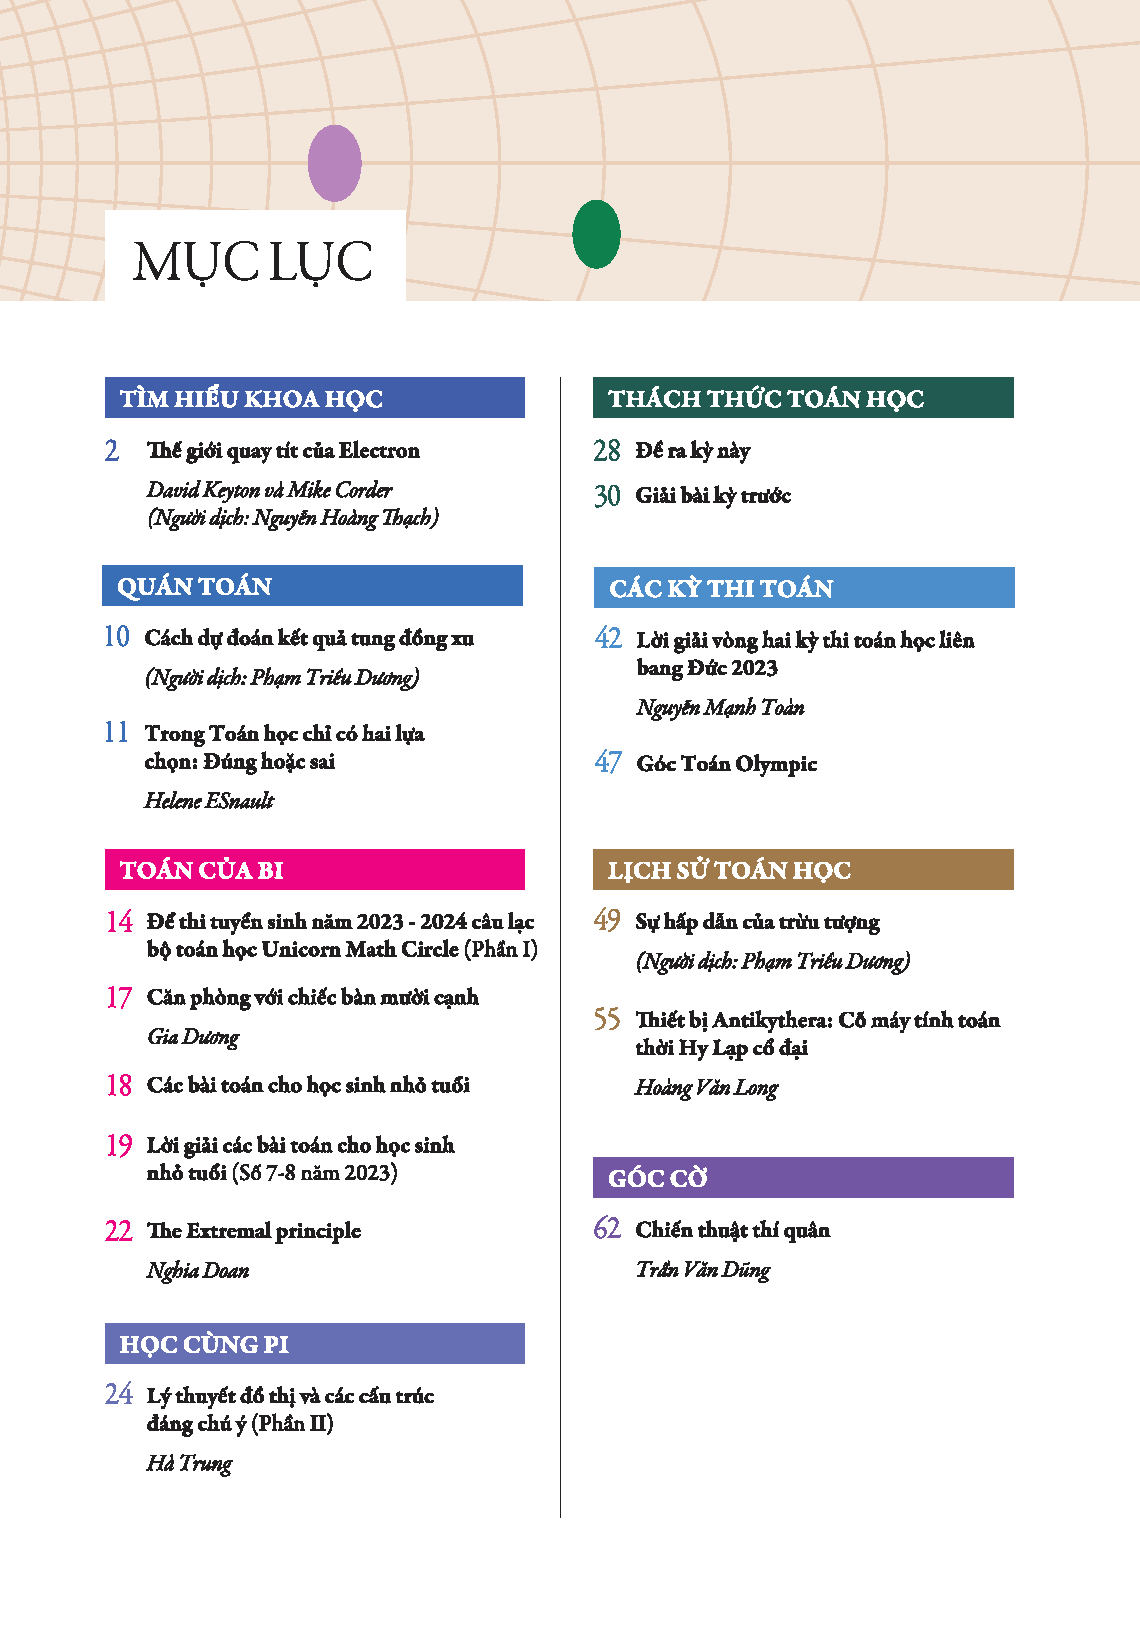
\includegraphics[scale=1]{ML.pdf}}}
	 \centering
	 \vspace*{0cm}
	 \endgroup
	 \newpage	  
	 \pagestyle{empty}

	\setcounter{page}{2}

	\setcounter{figure}{0}
	\thispagestyle{timhieukhoahocnone}
\pagestyle{timhieukhoahoc}
\everymath{\color{timhieukhoahoc}}
\blfootnote{$^1$\text{\color{timhieukhoahoc}https://phys.org/news/2023-10-scientists-nobel-prize-physics-electrons.html}}
\blfootnote{$^2$\text{\color{timhieukhoahoc}Viện Toán học.}}

\graphicspath{{../timhieukhoahoc/pic/}}
\begingroup
\AddToShipoutPicture*{\put(0,616){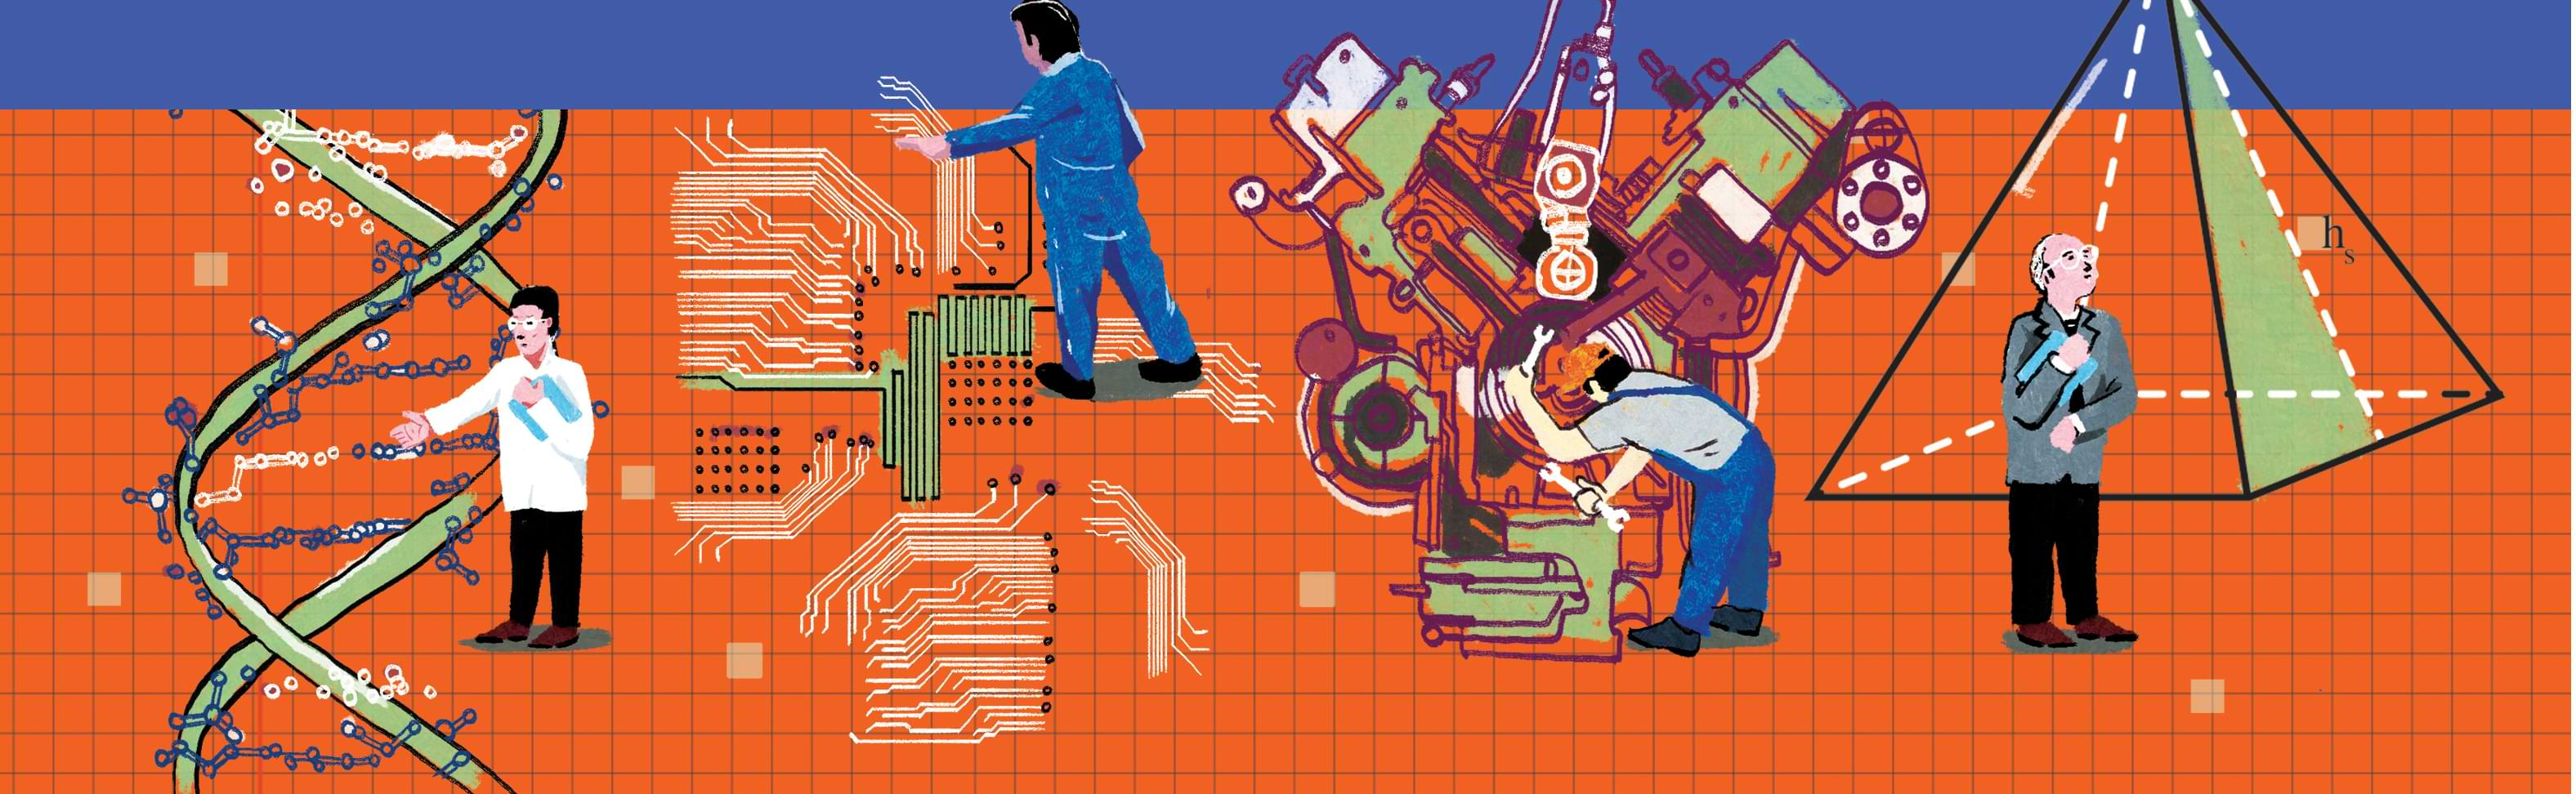
\includegraphics[width=19.3cm]{../bannertimhieu}}}
\AddToShipoutPicture*{\put(60,533){
\includegraphics[scale=1]{../tieude.pdf}}}
\centering
\endgroup
\vspace*{170pt}

\begin{multicols}{2}
	Hôm thứ ba ngày $3$ tháng $10$ vừa qua, ba nhà khoa học đã giành được Giải Nobel Vật lý $2023$ nhờ mang đến cho chúng ta cái nhìn đầu tiên về thế giới siêu tốc độ của các electron quay tít, một lĩnh vực có thể sẽ giúp cải tiến các thiết bị điện tử hoặc chẩn đoán bệnh.
	\begin{figure}[H]
		\vspace*{-5pt}
		\centering
		\captionsetup{labelformat= empty, justification=centering}
		
\includegraphics[width= 1\linewidth]{1}
		\caption{\small\textit{\color{timhieukhoahoc}Ảnh: Viện Hàn lâm Khoa học Hoàng gia Thụy~Điển.}}
		\vspace*{-10pt}
	\end{figure}
	Giải thưởng được trao cho nhà vật lý Pháp -- Thụy Điển Anne L'Huillier, nhà vật lý người Pháp Pierre Agostini và nhà vật lý gốc Hungary Ferenc Krausz, vì công trình của họ về thành phần tí hon chạy quanh hạt nhân của nguyên tử và là cái cơ bản của hầu như mọi thứ: hóa học, vật lý, cơ thể và vật dụng của chúng ta.
	\vskip 0.1cm
	Theo các chuyên gia, electron di chuyển nhanh đến nỗi con người không thể cô lập được chúng, nhưng bằng cách quan sát trong những tích tắc nhỏ nhất có thể, các nhà khoa học hiện đã có cái nhìn thoáng qua ``mờ mờ" về chúng, qua đó mở ra nhiều ngành khoa học hoàn toàn mới.
	\vskip 0.1cm
	``Electron di chuyển rất nhanh, và chúng thực sự là lực lượng lao động ở mọi nơi," Mats Larsson, thành viên Ủy ban Giải thưởng Nobel, cho biết. ``Một khi có thể điều khiển và hiểu được electron, bạn đã tiến được một bước lớn."
	\vskip 0.1cm
	L'Huillier, giáo sư tại Đại học Lund, Thụy Điển, là người phụ nữ thứ năm được Nobel Vật lý.
	\vskip 0.1cm
	``Gửi đến tất cả phụ nữ, tôi muốn nói rằng nếu bạn thích, nếu bạn có một chút đam mê với những thách thức kiểu này, hãy theo đuổi nó," bà nói với hãng tin AP.
	\vskip 0.1cm
	\textbf{\color{timhieukhoahoc}Khám phá được trao Giải Nobel Vật lý}
	\vskip 0.1cm
	Ba nhà khoa học, độc lập với nhau, đã sử dụng xung laser ngày càng nhanh để bắt lại hoạt động của nguyên tử xảy ra ở tốc độ chóng mặt -- một phần tỷ tỷ giây, hay một \textit{atto} giây\footnote[3]{\color{timhieukhoahoc}$1$ atto giây = $10^{-18}$ giây -- Pi.} -- giống như cách các nhiếp ảnh gia sửa dụng cửa trập tốc độ cao để chụp ảnh chim ruồi đang hút mật hoa.
	\begin{figure}[H]
		\vspace*{5pt}
		\centering
		\captionsetup{labelformat= empty, justification=centering}
		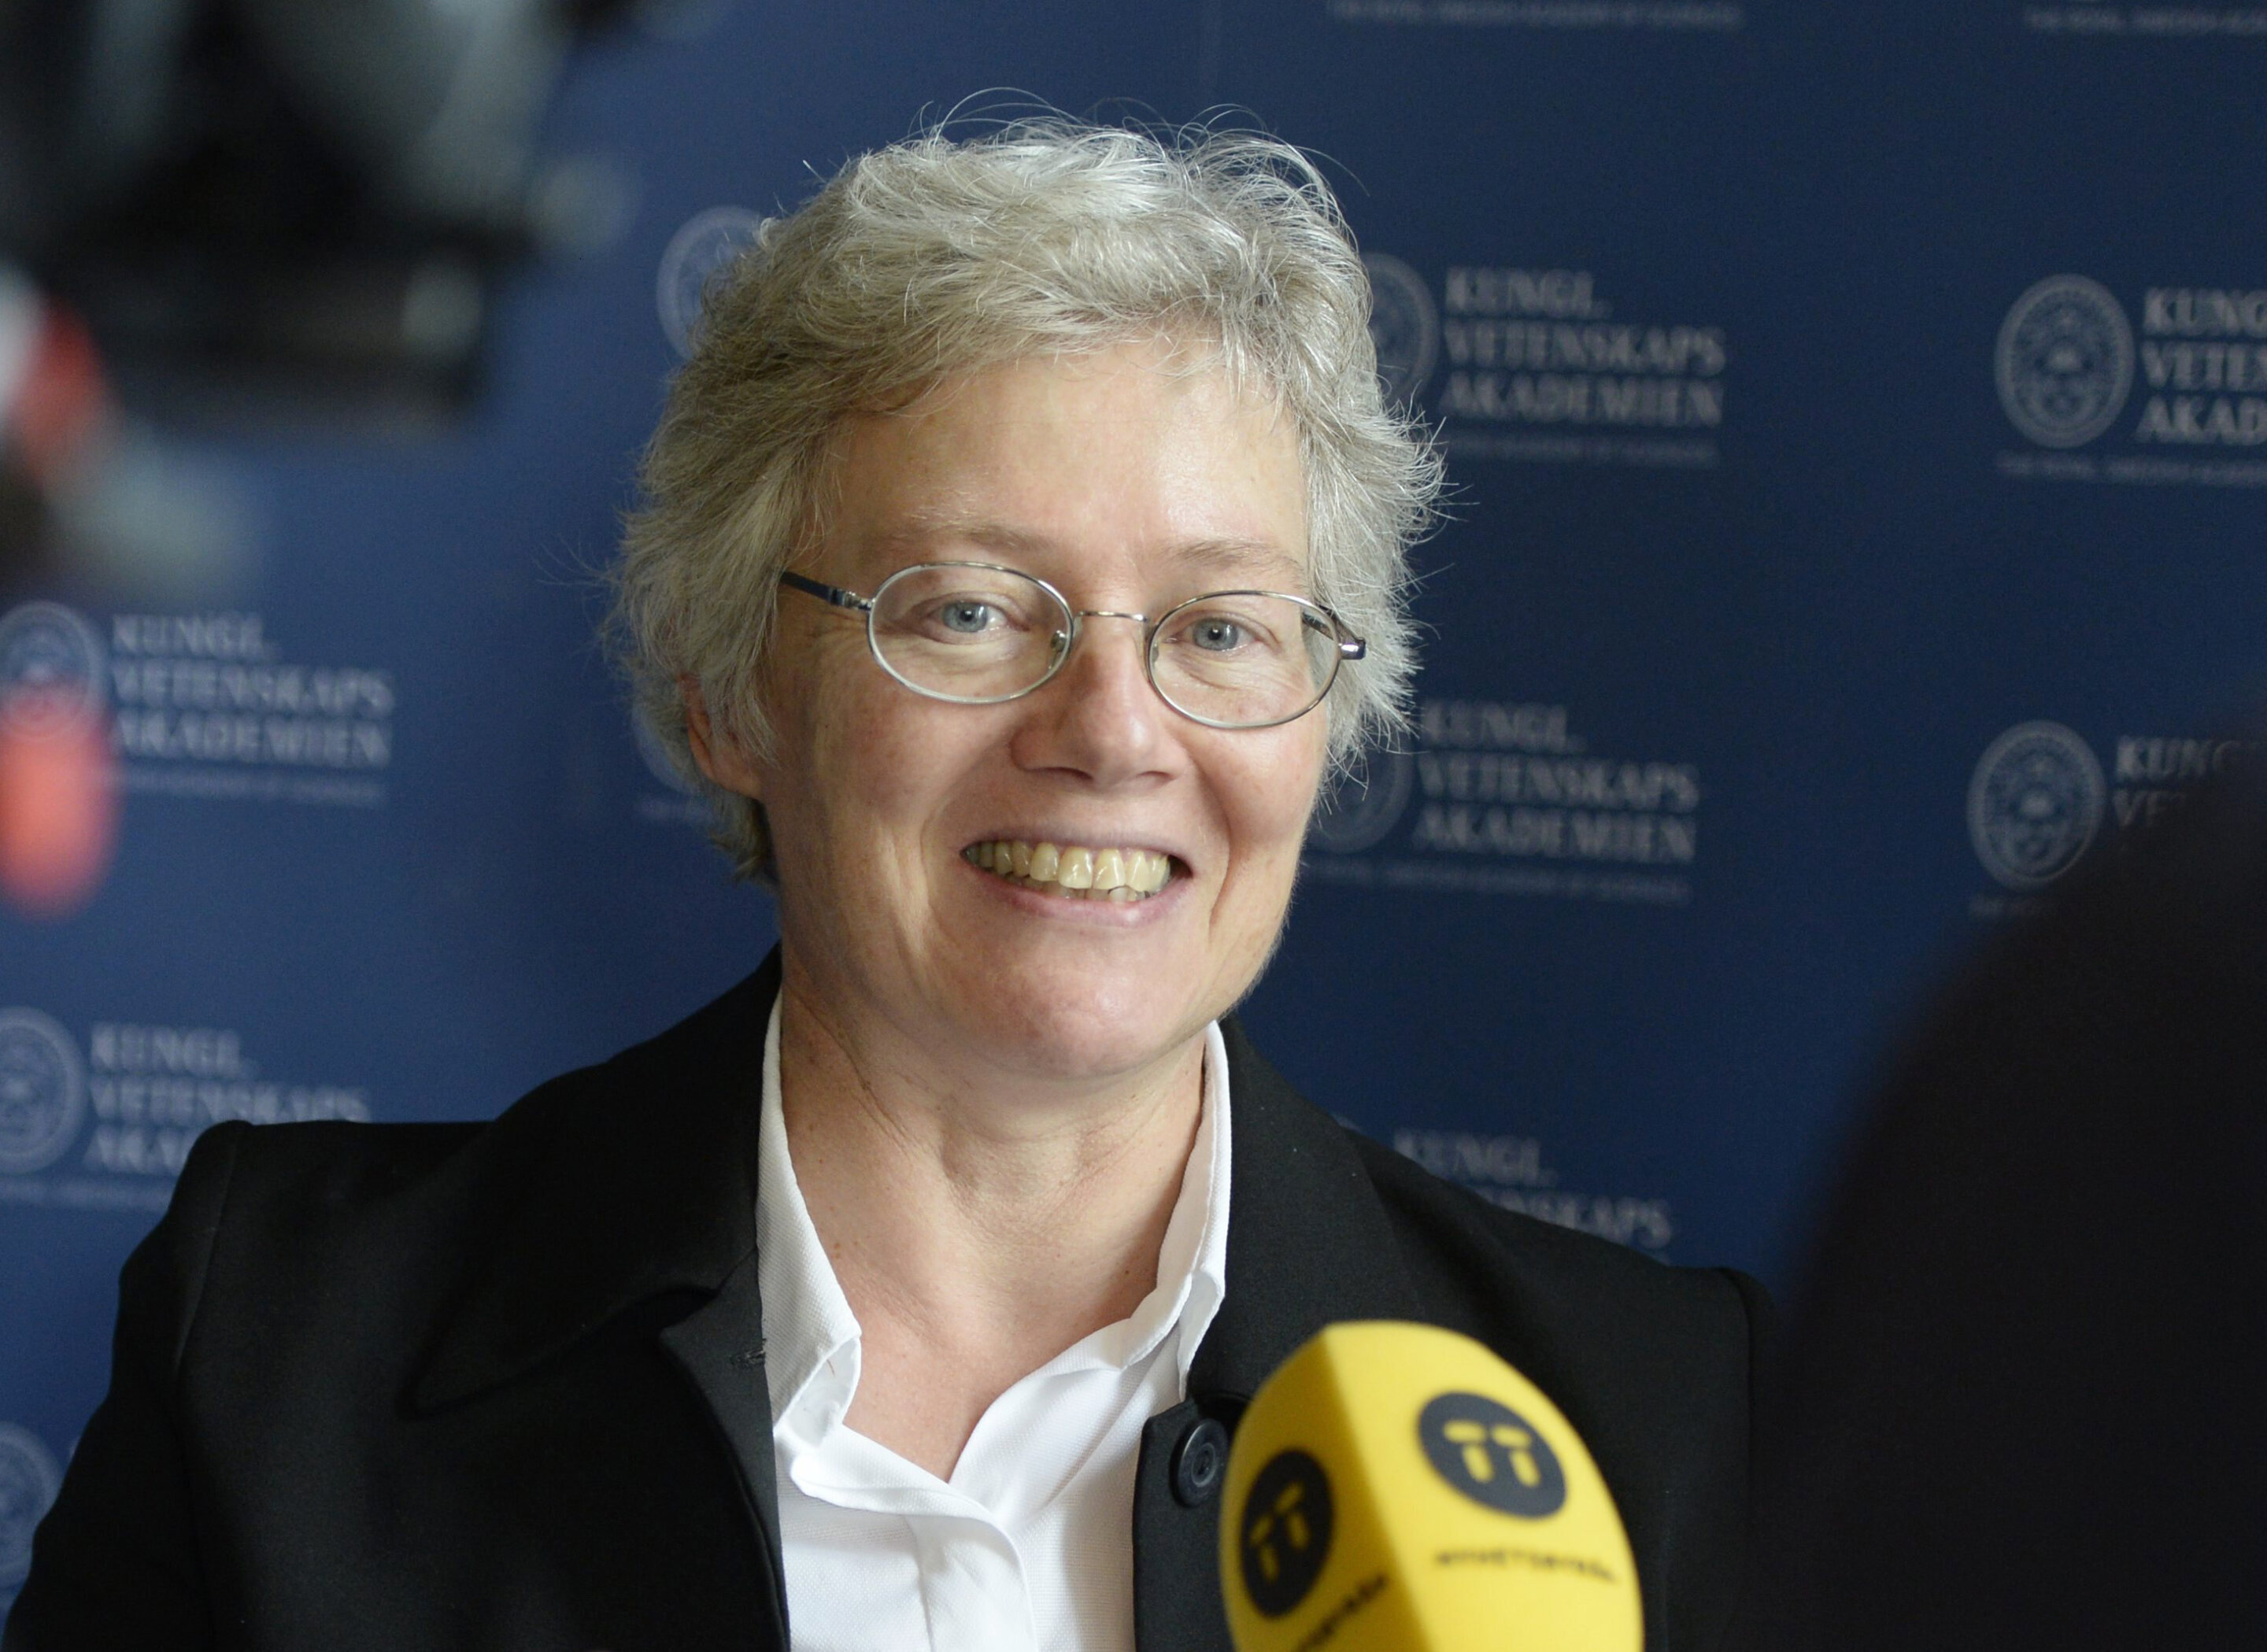
\includegraphics[width= 1\linewidth]{3}
		\caption{\small\textit{\color{timhieukhoahoc}Nhà vật lý Pháp--Thụy Điển Anne L'Huillier}}
		\vspace*{-10pt}
	\end{figure}
	Khoảng thời gian đó ngắn đến mức nào?
	\vskip 0.1cm
	``Hãy lấy một giây, là khoảng thời gian của một nhịp tim," chủ tịch Ủy ban Giải thưởng Nobel, Eva Olsson nói. Để đạt đến cỡ atto giây, cần chia nó cho $1000$ sáu lần.
	\vskip 0.1cm
	Nhà vật lý Mark Pearce, thành viên Ủy ban Giải thưởng Nobel, nói rằng ``số atto giây trong một giây bằng số giây đã trôi qua kể từ Big Bang, khoảng $13{,}8$ tỷ năm trước."
	\vskip 0.1cm
	Nhưng ngay cả khi ``thấy" được electron, các nhà khoa học cũng không thấy được hết.
	\vskip 0.1cm
	``Bạn có thể thấy nó ở phía bên này hay phía bên kia của một phân tử," L'Huillier, năm nay $65$ tuổi, nói. ``Nó vẫn rất mờ."
	\vskip 0.1cm
	``Electron giống sóng, như sóng trên mặt nước, nhiều hơn là giống hạt, và cái chúng tôi đo với kỹ thuật của mình là vị trí của ngọn sóng," bà nói thêm.
	\vskip 0.1cm
	\textbf{\color{timhieukhoahoc}Vì sao electron quan trọng?}
	\vskip 0.1cm
	Electron có vai trò then chốt vì chúng chính là ``cách các nguyên tử liên kết với nhau," L'Huillier nói. Đó là nơi diễn ra các phản ứng hóa học.
	\vskip 0.1cm
	``Dù ta không thể thấy chúng, electron hiện diện khắp mọi nơi trong cuộc sống của chúng ta, theo cả nghĩa cuộc sống sinh học lẫn cuộc sống kỹ thuật, cuộc sống hàng ngày," Krausz nói tại một buổi họp báo. ``Trong cuộc sống sinh học, electron tạo nên chất keo giữa các nguyên tử, từ đó các nguyên tử tạo thành phân tử, và các phân tử này là những viên gạch nhỏ nhất để xây dựng nên mọi cơ thể sống."
	\vskip 0.1cm
	Và nếu muốn hiểu cách chúng làm việc, bạn cần biết cách chúng di chuyển, Krausz nói.
	\vskip 0.1cm
	Hiện tại, khoa học này phục vụ cho việc tìm hiểu vũ trụ của chúng ta, nhưng người ta hy vọng nó cuối cùng sẽ có ứng dụng thực tế trong điện tử, chẩn đoán bệnh và hóa học cơ bản.
	\vskip 0.1cm
	L'Huillier nói rằng công trình của bà cho thấy tầm quan trọng của việc tiến hành nghiên cứu cơ bản mà không cần biết có ứng dụng trong tương lai hay không: bà đã làm việc với nó $30$ năm trước khi những ứng dụng thực tế trở nên rõ ràng hơn.
	\begin{figure}[H]
		\vspace*{-5pt}
		\centering
		\captionsetup{labelformat= empty, justification=centering}
		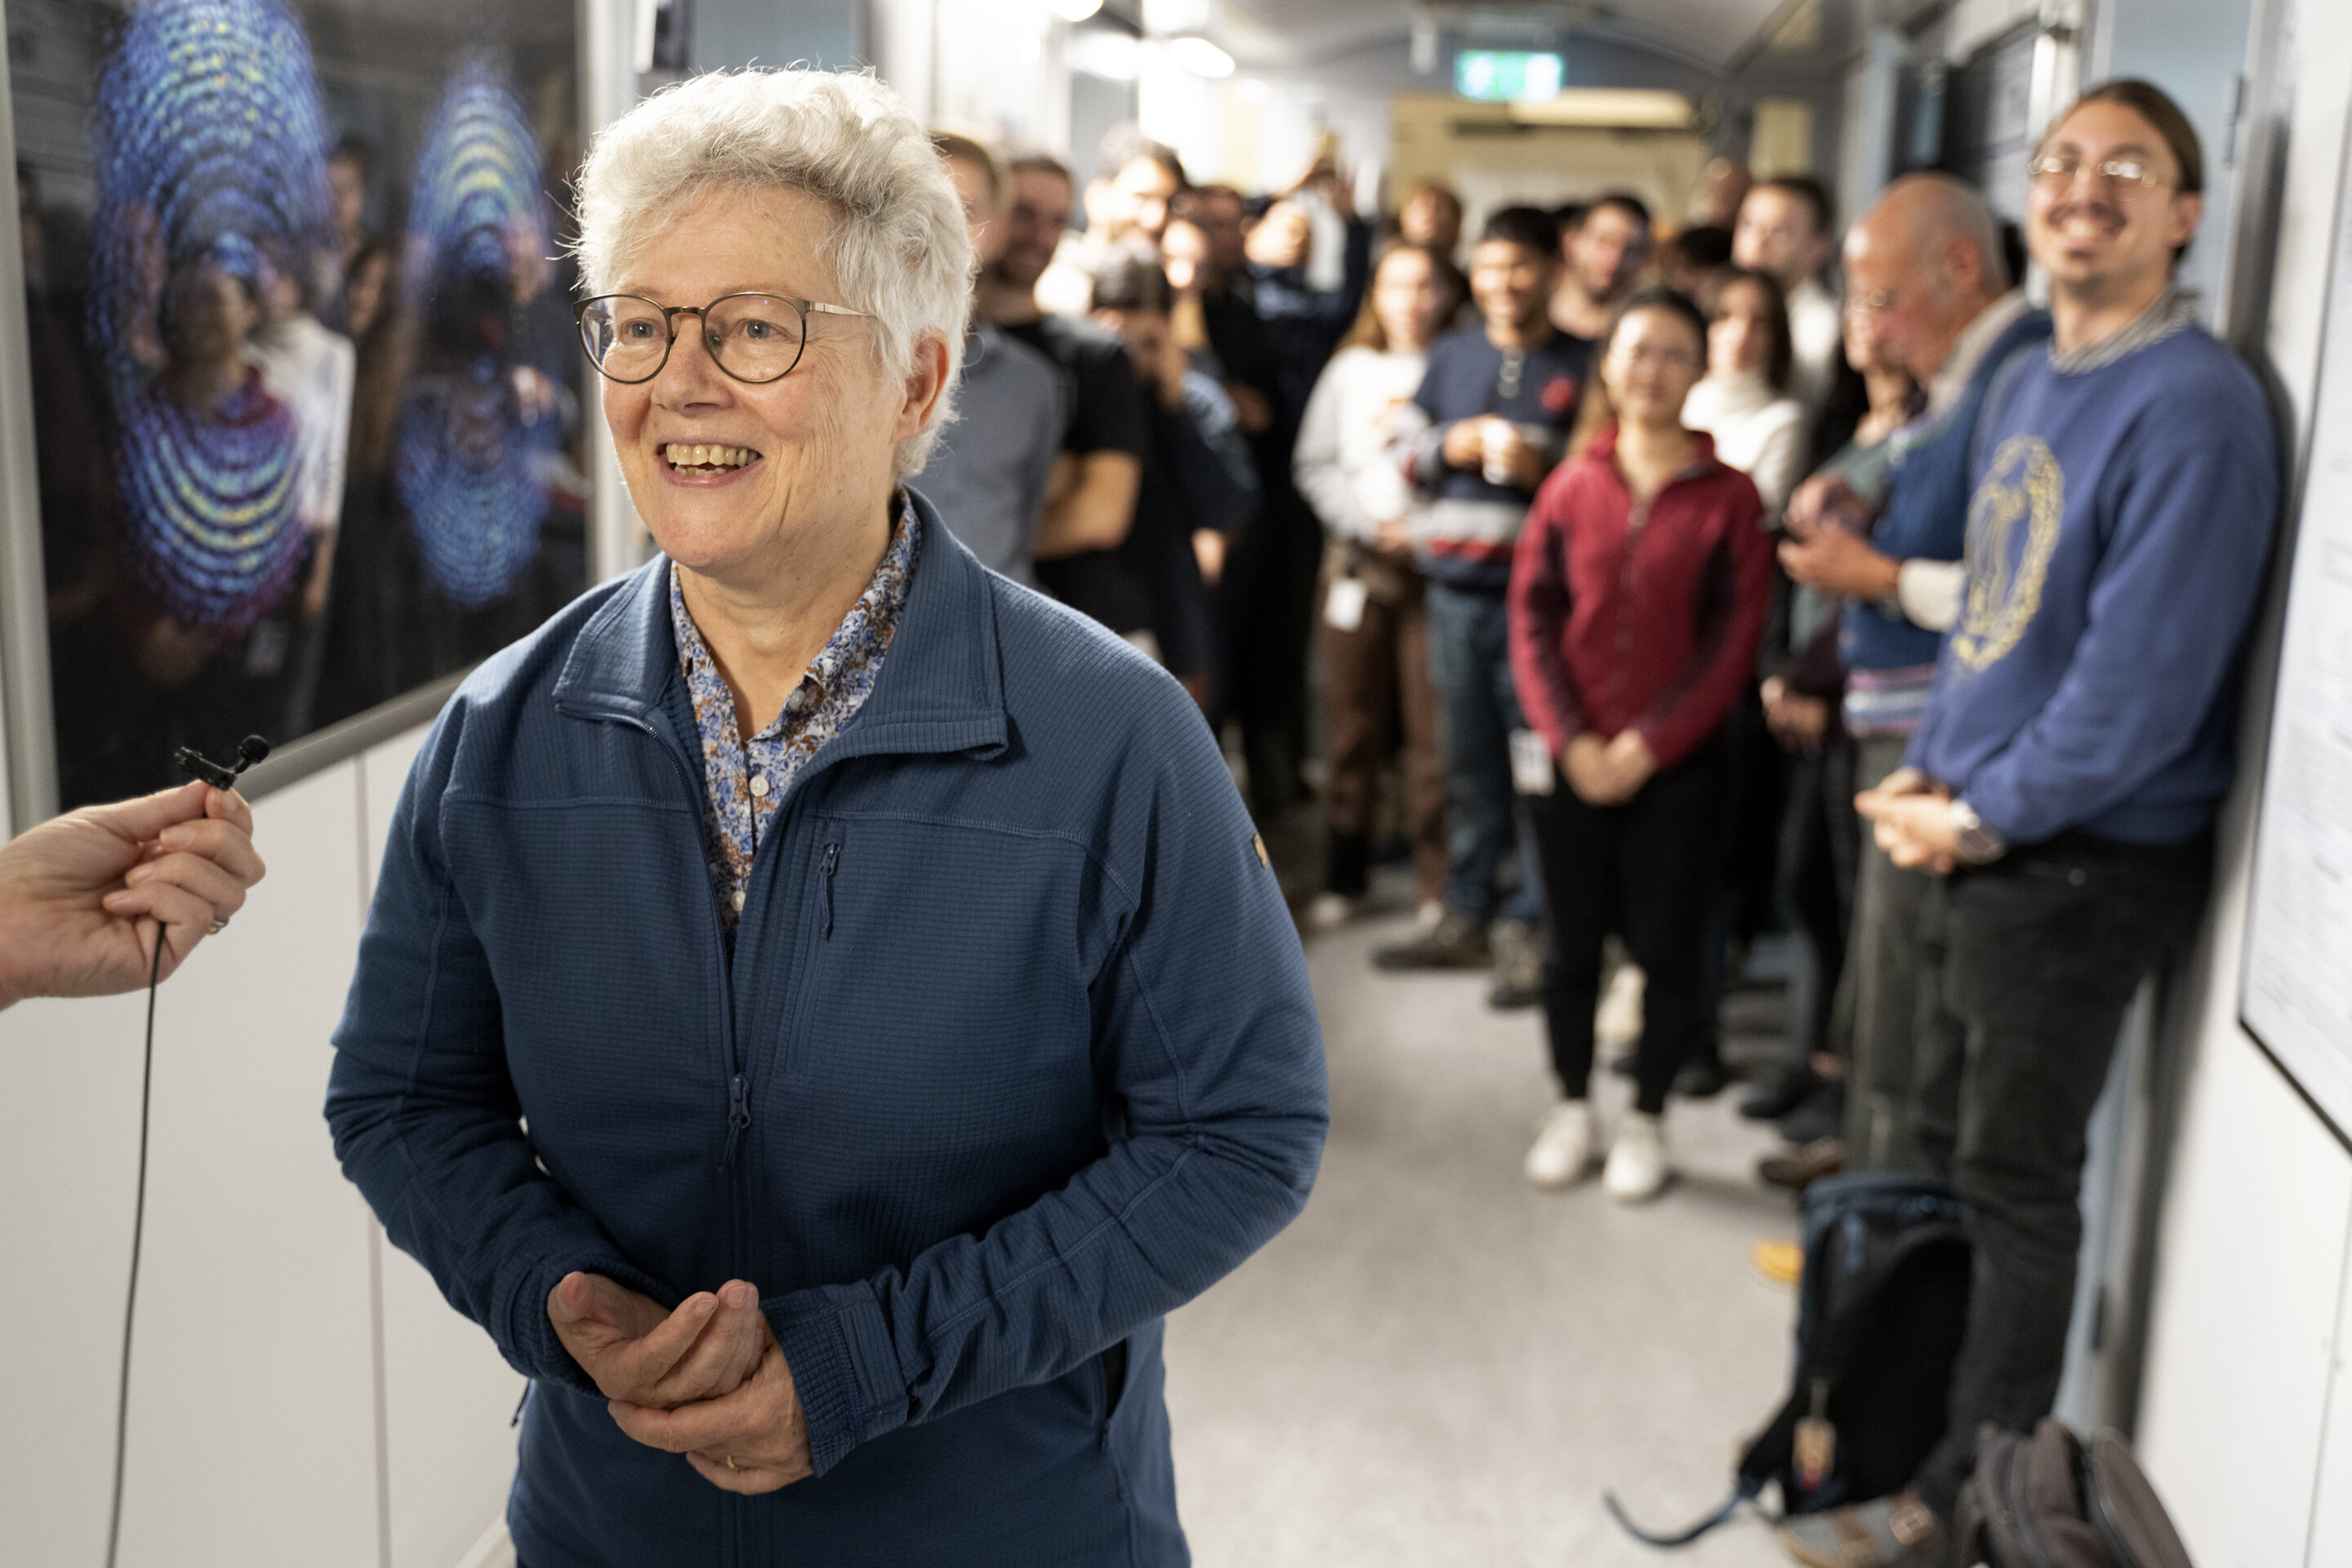
\includegraphics[width= 1\linewidth]{2}
		\caption{\small\textit{\color{timhieukhoahoc}Anne L'Huillier trả lời phỏng vấn tại Đại học Lund, Lund, Thụy Điển hôm thứ ba $3/10/2023$.}}
		\vspace*{-10pt}
	\end{figure}
%	\end{figure}
%	\begin{figure}[H]
%		\vspace*{-5pt}
%		\centering
%		\captionsetup{labelformat= empty, justification=centering}
%		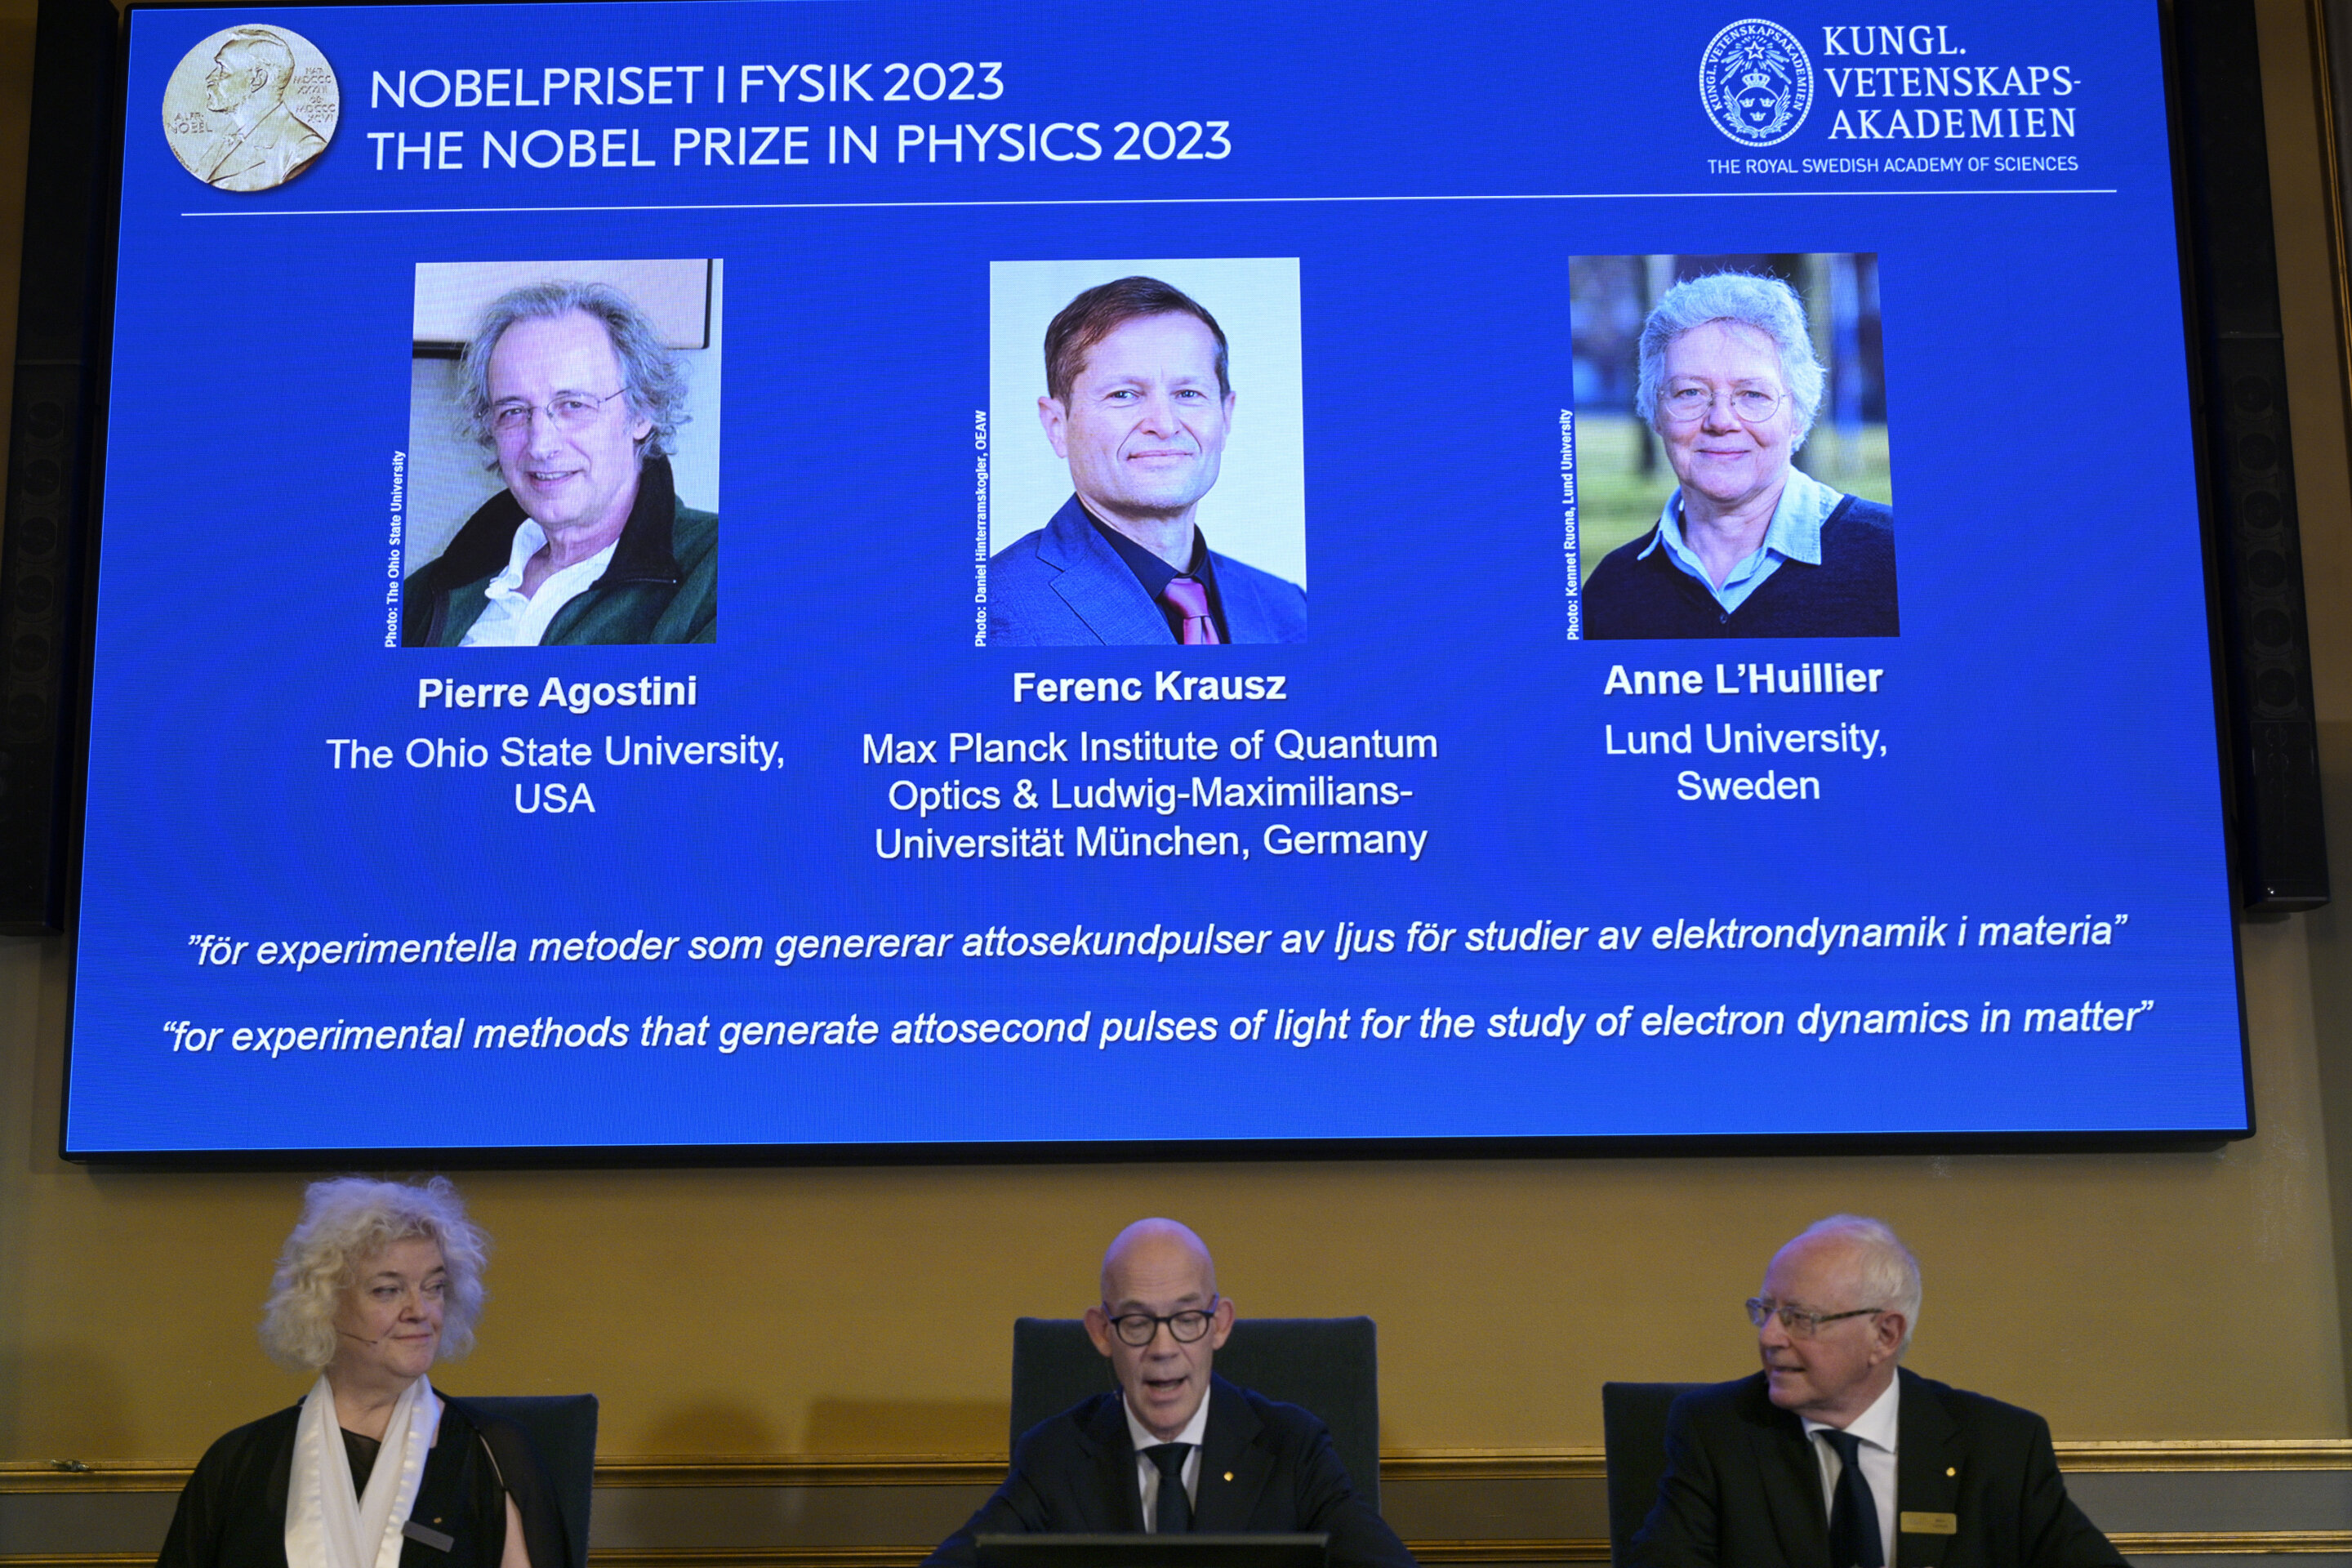
\includegraphics[width= 1\linewidth]{4}
%		%		\caption{\small\textit{\color{}}}
%		\vspace*{-15pt}
%	\end{figure}
	\textbf{\color{timhieukhoahoc}Phản ứng của ba nhà khoa học}
	\vskip 0.1cm
	Khi nhận được cuộc gọi báo tin được giải thưởng, L'Huillier đang dạy vật lý cơ bản dành cho kỹ sư cho khoảng $100$ sinh viên tại Lund; điện thoại của bà để ở chế độ im lặng và bà không nghe máy. Bà kiểm tra điện thoại trong giờ giải lao và gọi lại cho Ủy ban Giải thưởng Nobel.
	\vskip 0.1cm
	Sau đó bà quay lại dạy tiếp.
	\vskip 0.1cm
	``Lúc ấy tôi đang rất tập trung, tôi quên đi Giải Nobel và cố kết thúc bài giảng của mình," bà nói với AP. Bà kết thúc bài giảng sớm một chút để có thể trả lời họp báo công bố giải thưởng tại Viện Hàn lâm Khoa học Hoàng gia Thụy Điển ở Stockholm.
	\vskip 0.1cm
	``Đây là giải thưởng cao quý nhất và tôi thật hạnh phúc được nhận nó. Thật không thể tin được," bà nói ở buổi họp báo. ``Các bạn biết đấy, không có nhiều phụ nữ được giải này, bởi thế nó rất đặc biệt."
	\vskip 0.1cm
	Ban tổ chức giải Nobel đăng trên tài khoản mạng xã hội của mình một bức ảnh L'Huillier đang nghe điện thoại.
	\begin{figure}[H]
		\vspace*{-5pt}
		\centering
		\captionsetup{labelformat= empty, justification=centering}
		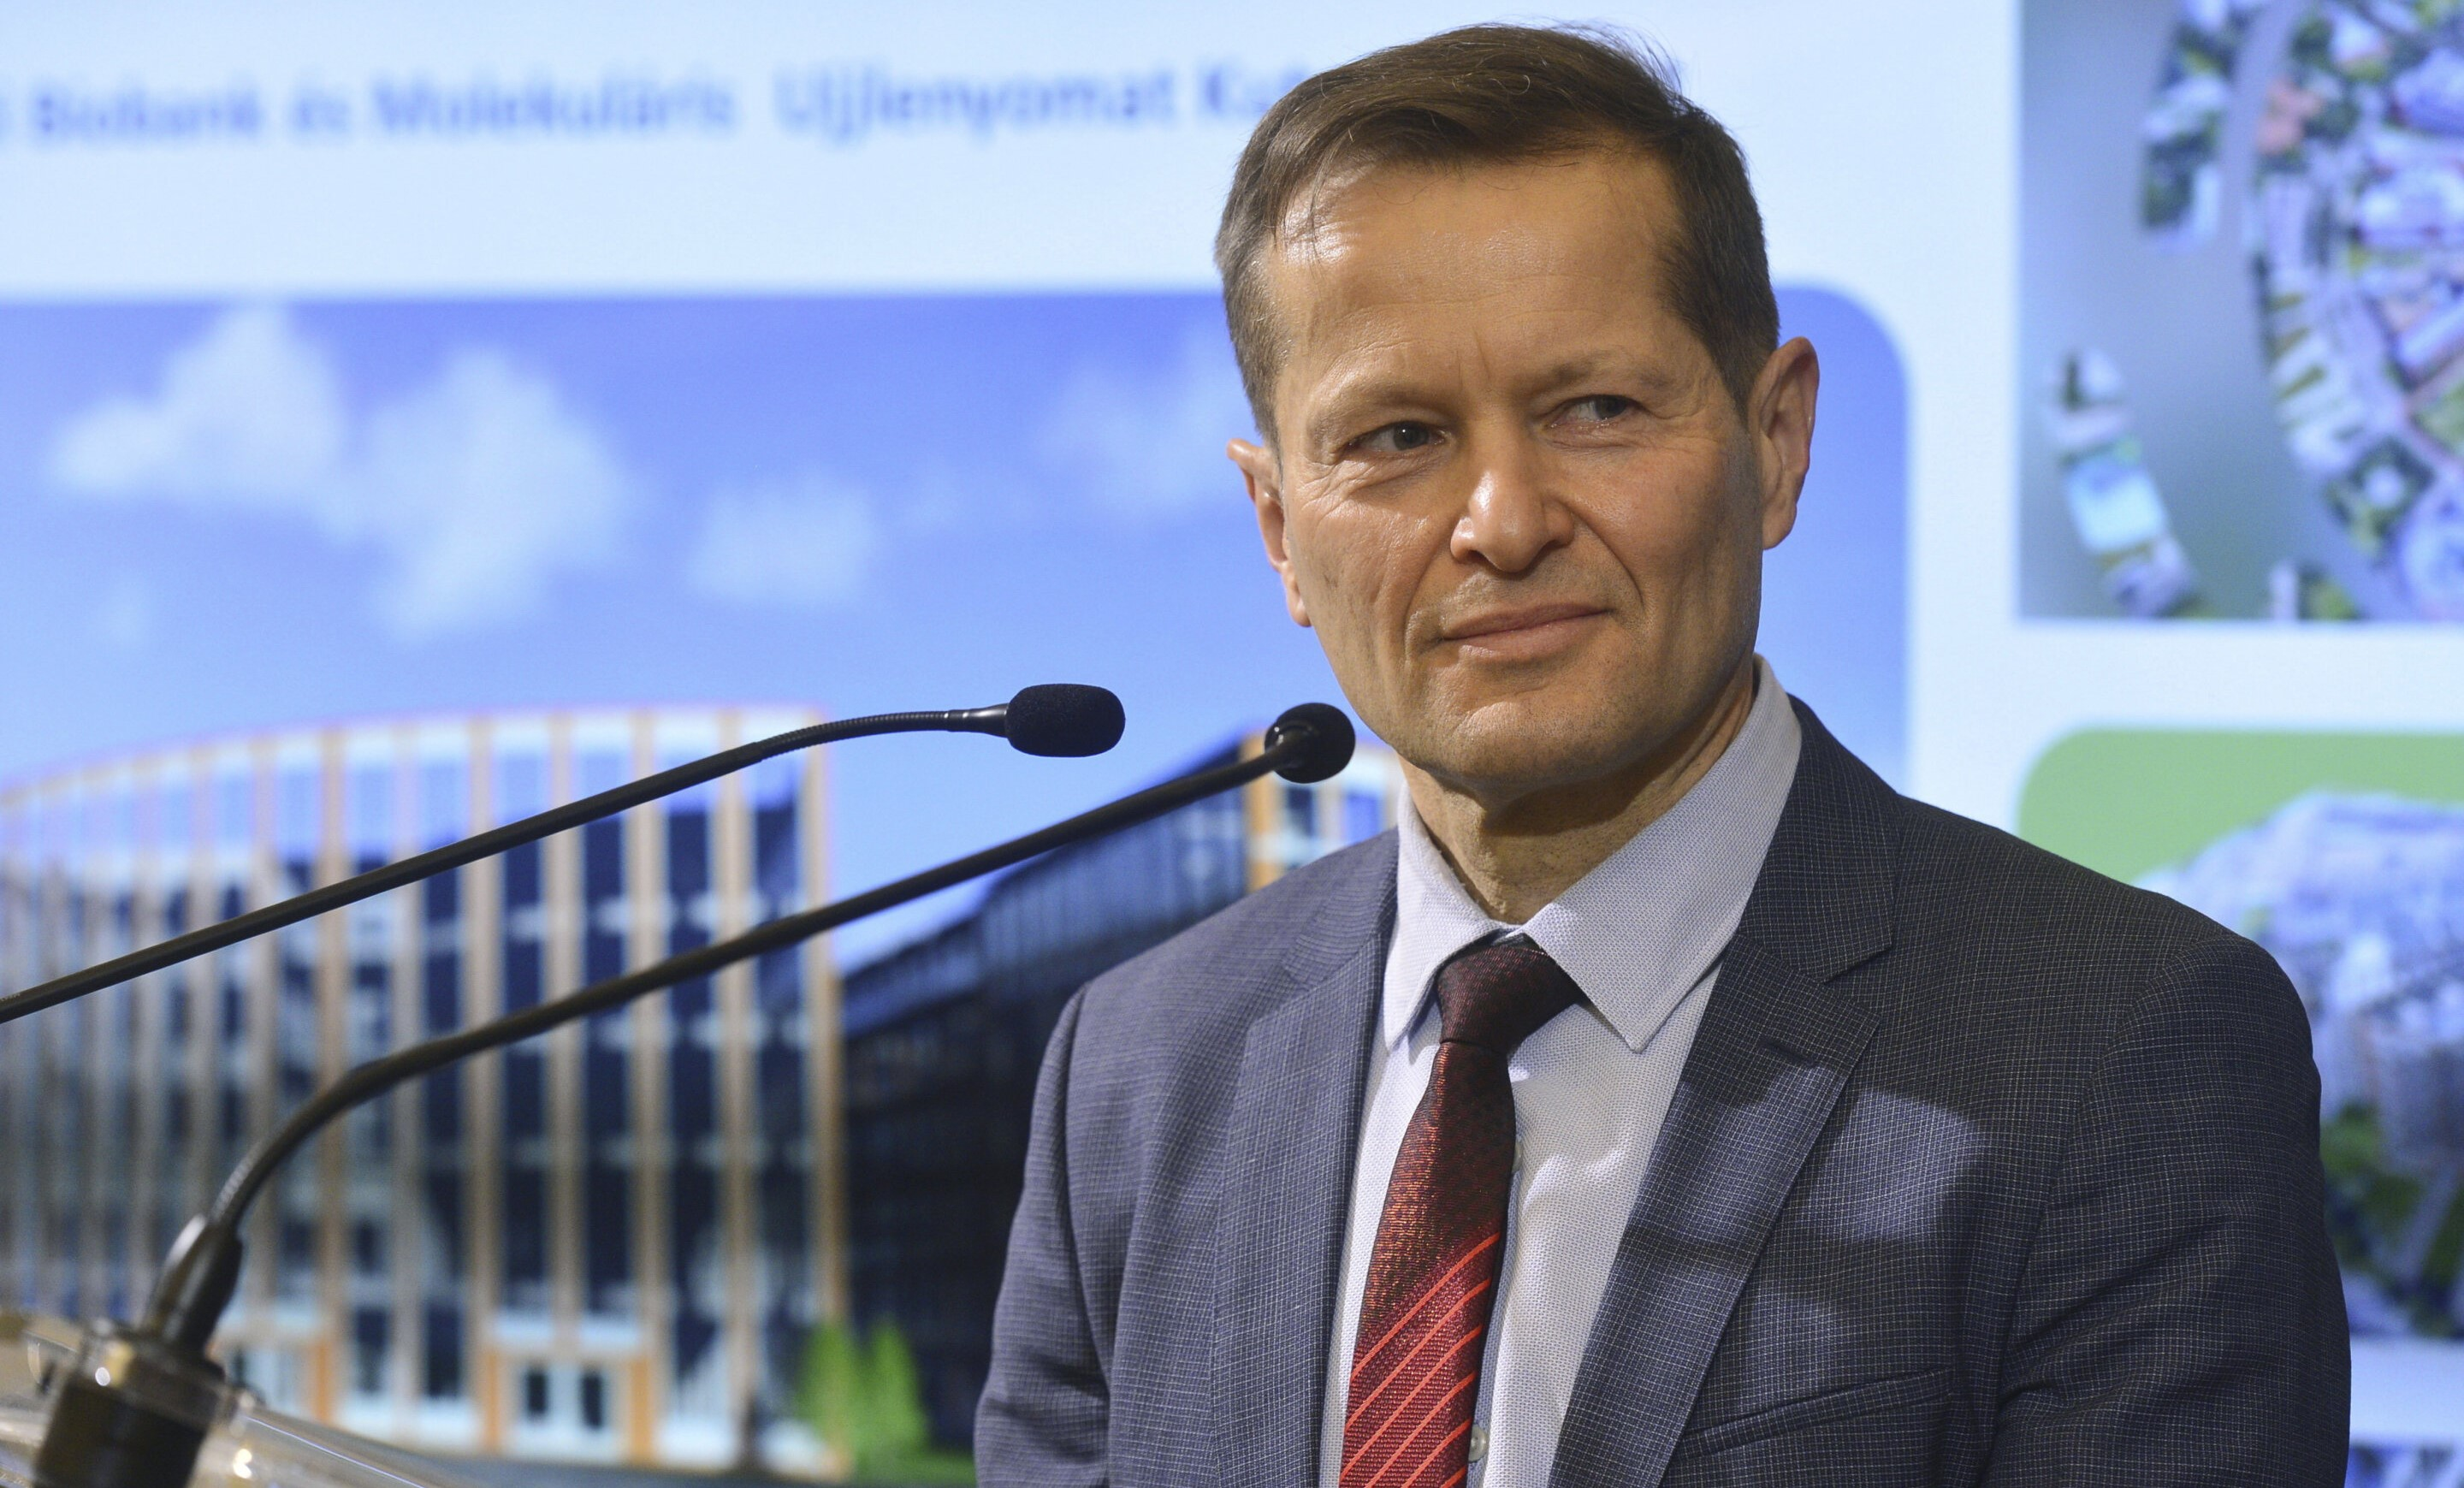
\includegraphics[width= 1\linewidth]{7}
		\caption{\small\textit{\color{timhieukhoahoc}Nhà vật lý người Hungary Ferenc Krausz.}}
		\vspace*{-10pt}
	\end{figure}
	``Cảnh báo: nhà giáo tận tâm!" bài đăng trên Twitter, nay là X, viết. ``Đến cả giải Nobel Vật lý $2023$ cũng không thể kéo Anne L'Huillier khỏi sinh viên của bà."
	\vskip 0.1cm
	Và L'Huillier cho biết khi đó vẫn phải giữ bí mật về giải thưởng nên bà không được phép giải thích với sinh viên, nhưng họ đoán được.
	\vskip 0.1cm
	Agostini, giáo sư danh dự tại Đại học Bang Ohio, khi đó đang ở Paris; Ủy ban Giải thưởng Nobel không liên lạc được với ông trước khi công bố việc ông được giải với cả thế giới.
	\vskip 0.1cm
	``Tôi không nhận được cuộc gọi nào từ ủy ban giải thưởng. Có lẽ không đúng. Tôi không biết," ông cười khi trả lời AP. ``Tôi nghĩ họ tìm tôi ở Columbus\footnote[4]{\color{timhieukhoahoc}Thủ phủ bang Ohio -- Pi.}."
	\vskip 0.1cm
	``Chắc chắn có nhiều người trẻ hơn đánh giá cao giải thưởng này hơn tôi," vị giáo sư $82$ tuổi nói đùa. ``Nó cũng tốt đấy, nhưng với tôi thì hơi muộn."
	\vskip 0.1cm
	Nhưng, ông nói thêm: ``Tôi không nghĩ mình sẽ xứng đáng nếu được trao giải sớm hơn!"
	\vskip 0.1cm
	Krausz, thuộc Viện Quang học Lượng tử Max Planck và Đại học Ludwig Maximilian tại Munich, nói với các phóng viên rằng ông bị choáng ngợp.
	\vskip 0.1cm
	``Từ $11$ giờ sáng đến giờ tôi vẫn đang nghĩ xem mình đang ở trong hiện thực hay trong một giấc mơ dài," nhà vật lý $61$ tuổi nói.
	\vskip 0.1cm
	Cuộc gọi từ ủy ban giải thưởng được hiển thị ``không có ID người gọi" và thường thì Krausz không nghe những cuộc gọi như vậy, nhưng lần này, ông ``nghĩ rằng mình sẽ thử nghe, và rõ ràng không thể dập máy ngay."
	\vskip 0.1cm
	Năm ngoái, cùng với nhà khoa học Paul Corkum của Đại học Ottawa, Krausz và L'Huillier được trao giải thưởng vật lý cao quý Wolf vì những công trình của họ. Giải Nobel chỉ được trao cho không quá ba người, và Krausz nói rằng thật đáng tiếc khi nó không thể được trao cho Corkum.
	\vskip 0.1cm
	Corkum là chìa khóa đối với cách đo các xung laser xảy ra trong tích tắc, và điều này mang tính cốt yếu, Krausz nói.
	\begin{figure}[H]
		\vspace*{-5pt}
		\centering
		\captionsetup{labelformat= empty, justification=centering}
		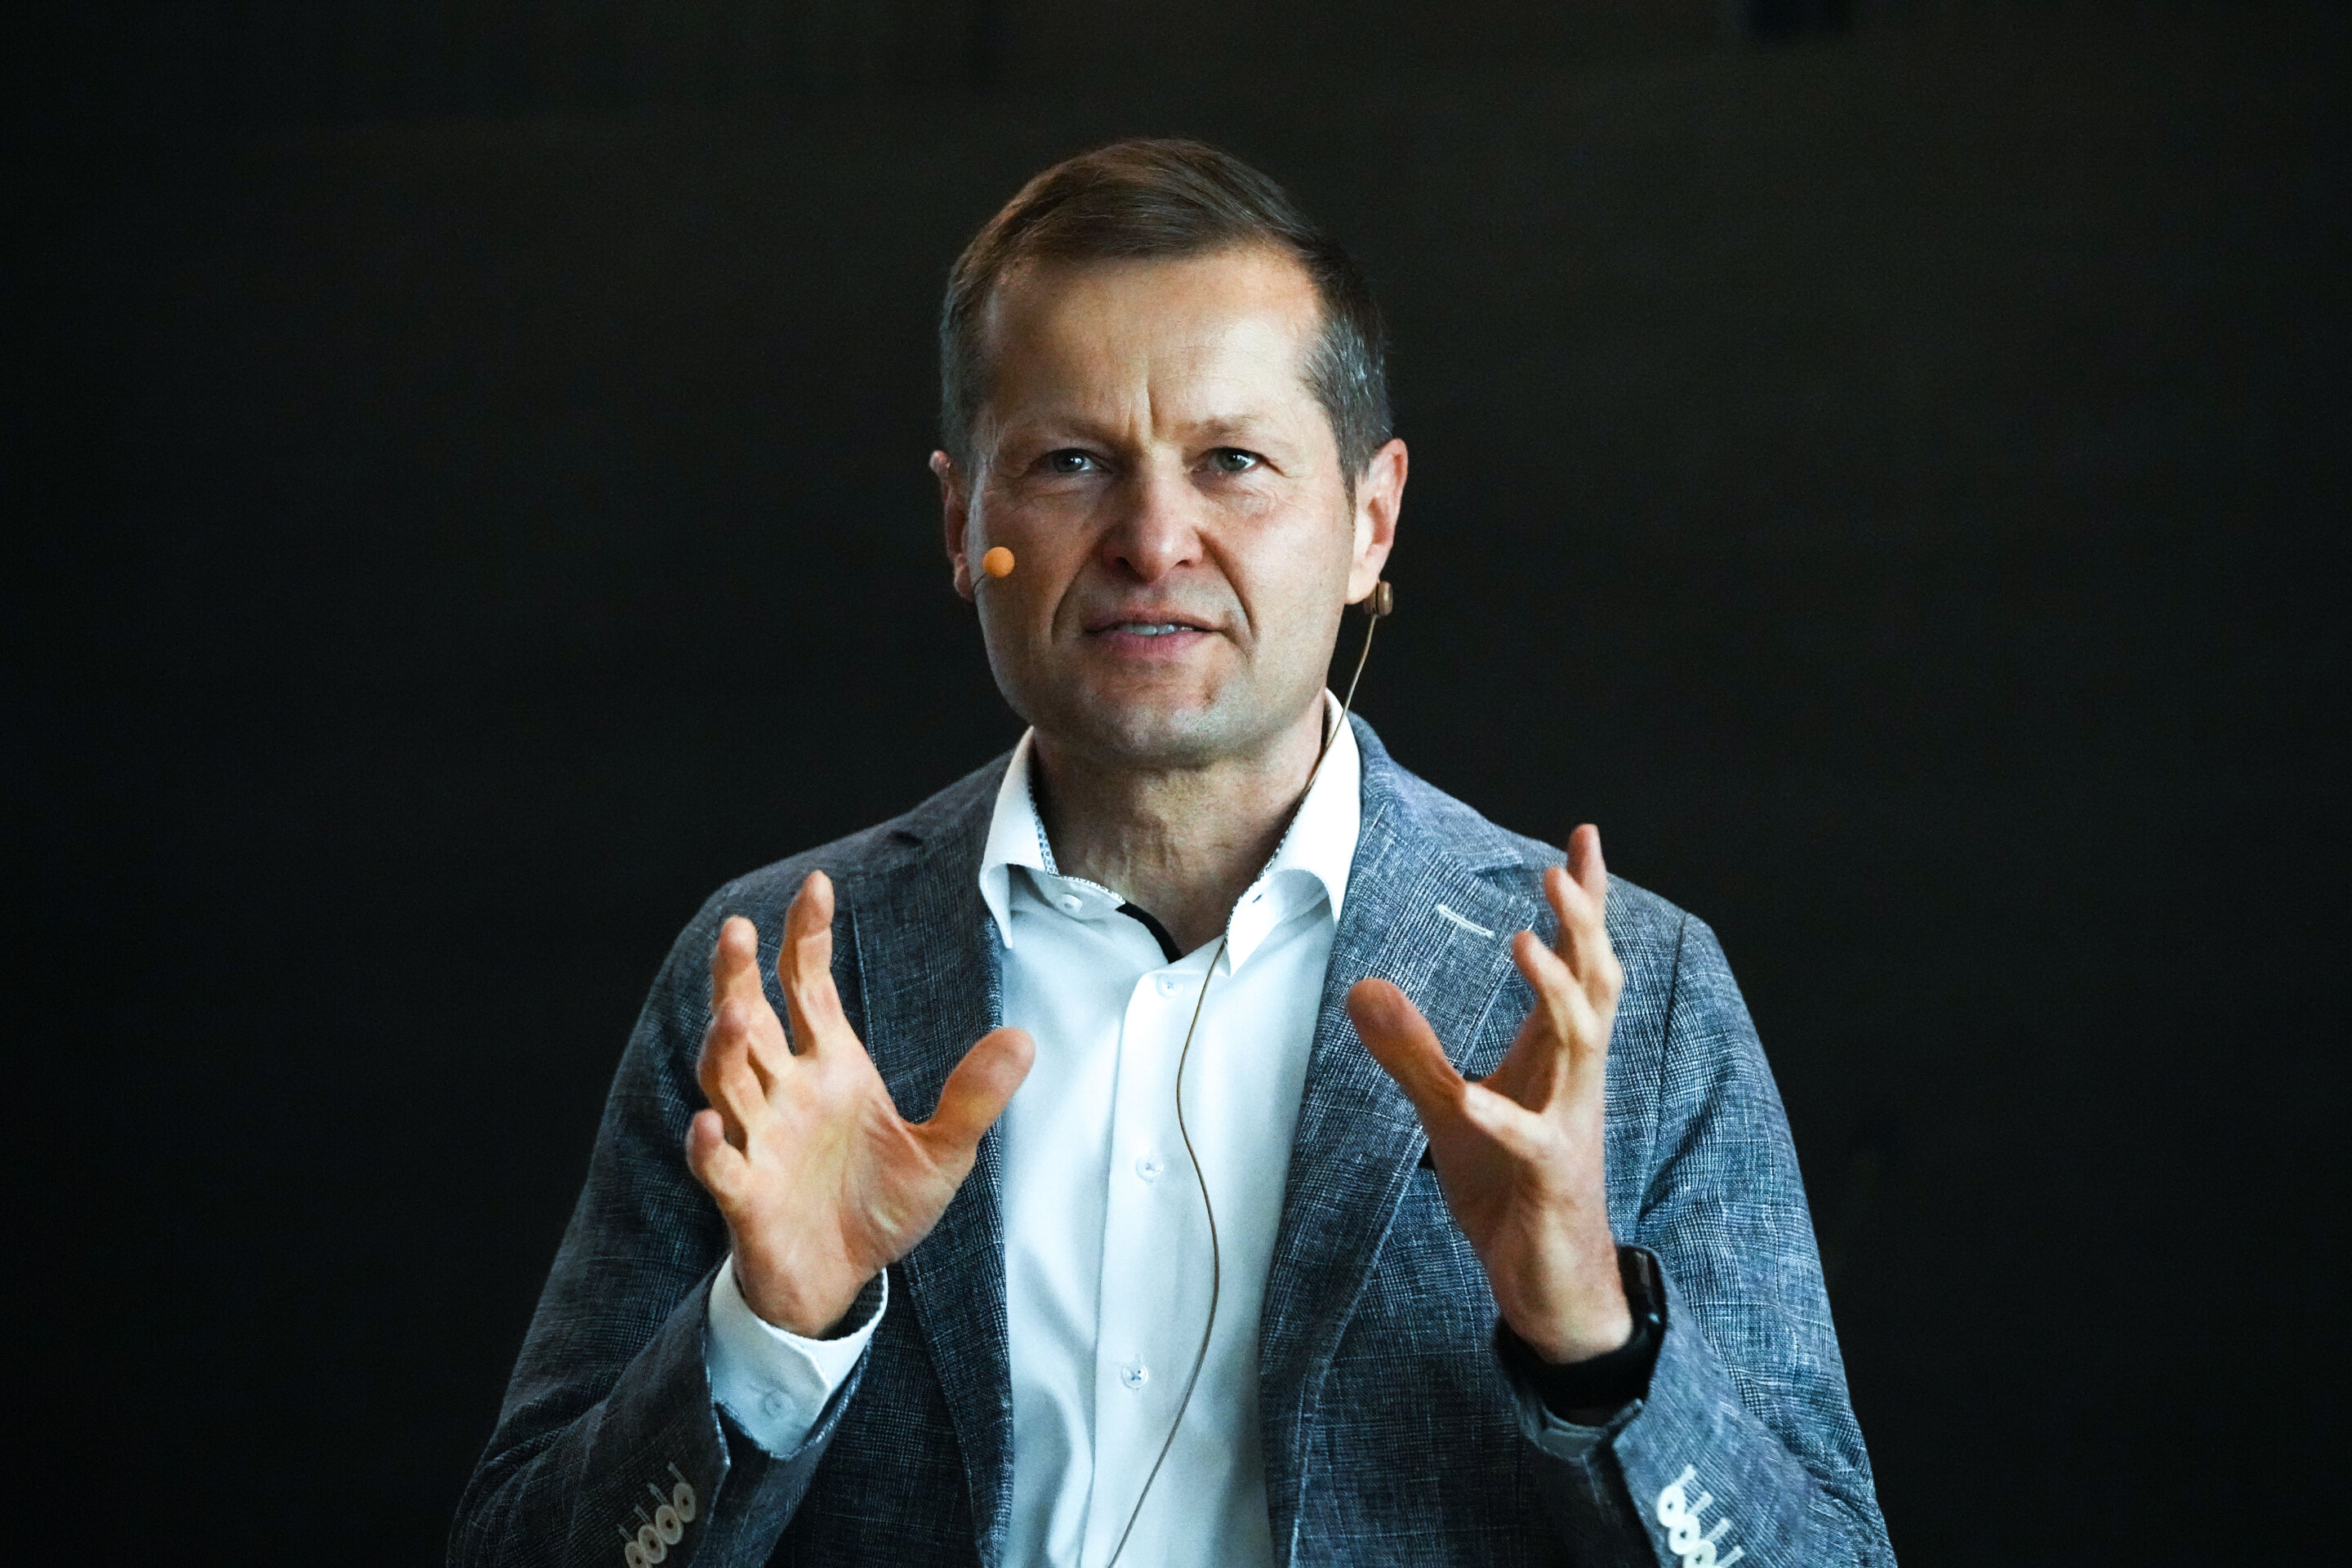
\includegraphics[width= 1\linewidth]{5}
		\caption{\small\textit{\color{timhieukhoahoc}Ferenc Krausz trong một buổi thuyết trình tại Viện Quang học Lượng tử Max Planck, Munich, Đức hôm thứ ba $3/10/2023$.}}
		\vspace*{-15pt}
	\end{figure}
	Giải Nobel có giá trị tiền thưởng khoảng $1$ triệu đô--la Mỹ, được trao theo di chúc của người sáng lập ra nó, nhà phát minh người Thụy Điển Alfred Nobel.
	\vskip 0.1cm
	Giải Nobel Vật lý được công bố một ngày sau khi hai nhà khoa học được giải Nobel Y học -- Sinh lý học vì những khám phá giúp tạo ra vaccine mRNA cho COVID--$19$.
	\vskip 0.1cm
	\textbf{\color{timhieukhoahoc}Thông báo của Ủy ban Giải thưởng Nobel:}
	\vskip 0.1cm
	Viện Hàn lâm Khoa học Hoàng gia Thụy Điển quyết định trao giải Nobel Vật lý $2023$ cho
	\vskip 0.1cm
	\textbf{\color{timhieukhoahoc}Pierre Agostini}, Đại học Bang Ohio, Columbus, Mỹ
	\vskip 0.1cm
	\textbf{\color{timhieukhoahoc}Ferenc Krausz},  Viện Quang học Lượng tử Max Planck, Garching và Đại học Ludwig Maximilian tại Munich, Đức
	\vskip 0.1cm
	\textbf{\color{timhieukhoahoc}Anne L'Huillier}, Đại học Lund, Thụy Điển
	\vskip 0.1cm
	``vì các phương pháp thực nghiệm tạo ra các xung ánh sáng atto giây nhằm nghiên cứu động lực học của electron trong vật chất".
	\begin{figure}[H]
		\vspace*{-5pt}
		\centering
		\captionsetup{labelformat= empty, justification=centering}
		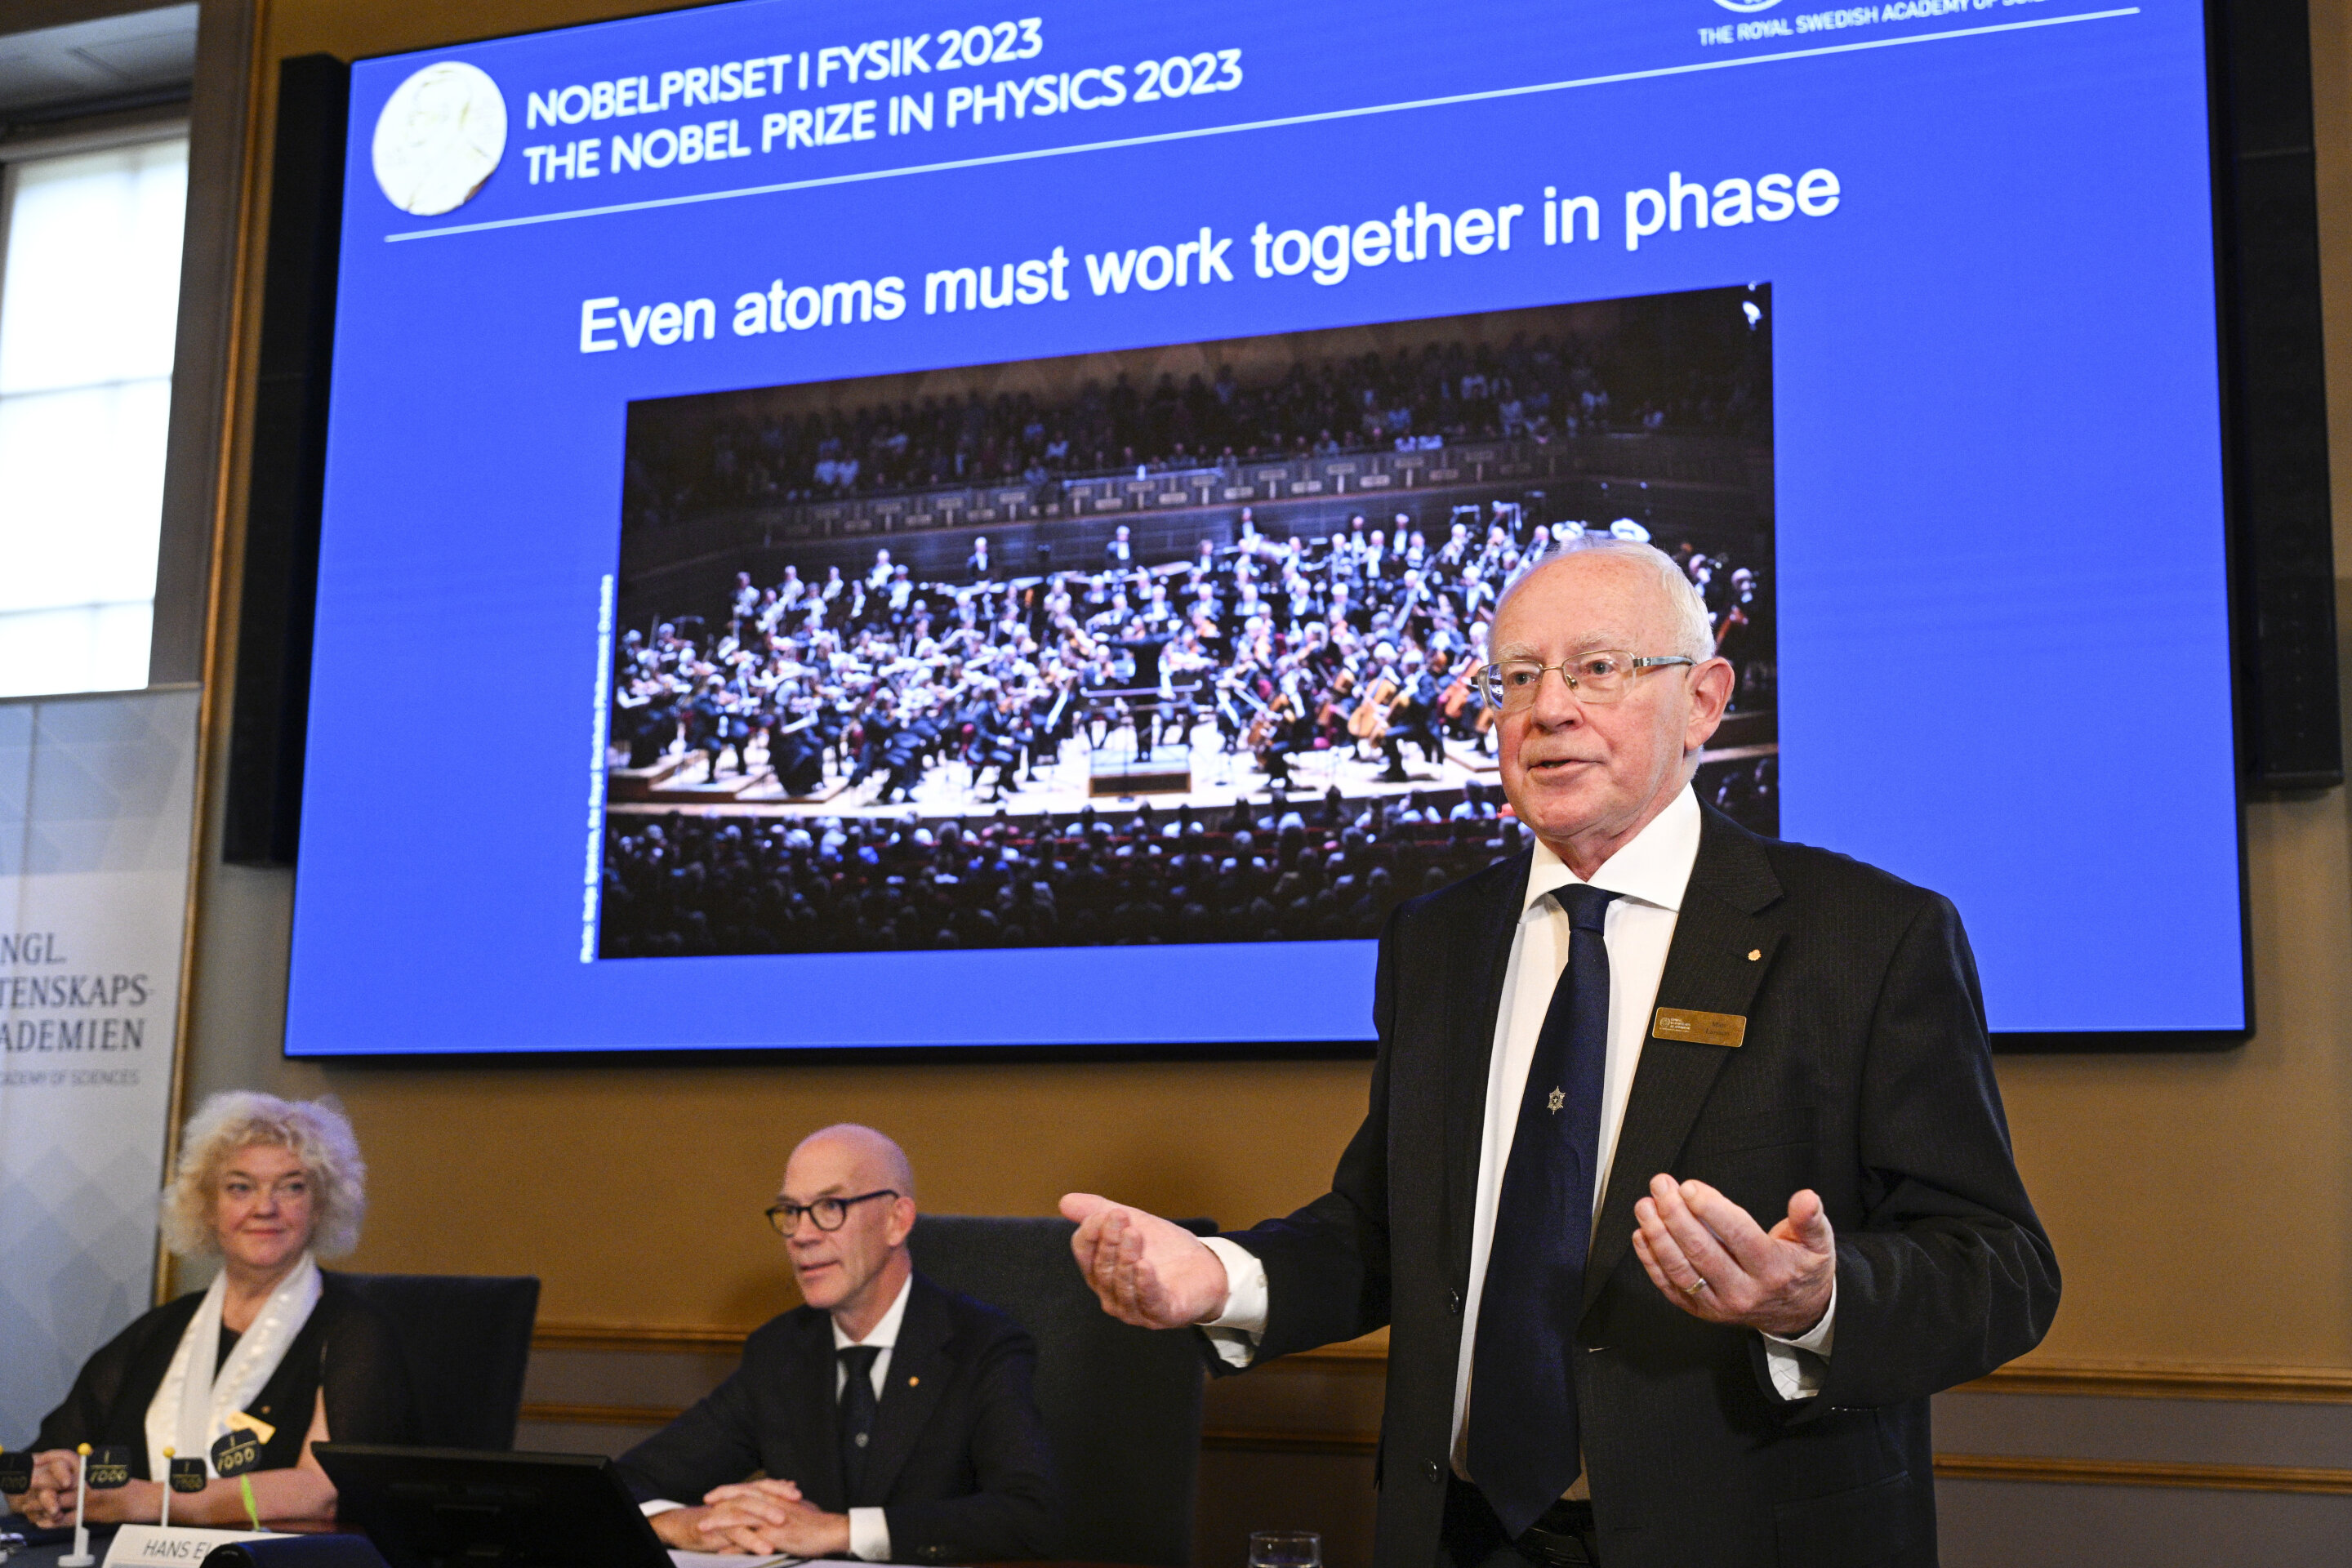
\includegraphics[width= 1\linewidth]{9}
%		\caption{\small\textit{\color{}}}
		\vspace*{-15pt}
	\end{figure}
	\textbf{\color{timhieukhoahoc}Thí nghiệm với ánh sáng bắt được những khoảnh khắc ngắn nhất}
	\vskip 0.1cm
	Ba nhà khoa học được giải Nobel Vật lý $2023$ được vinh danh vì những thí nghiệm cung cấp cho nhân loại những công cụ mới để khám phá thế giới của electron bên trong nguyên tử và phân tử. Pierre Agostini, Ferenc Krausz và Anne L'Huillier đã trình bày một cách tạo ra những xung ánh sáng cực ngắn có thể được dùng để đo các quá trình rất nhanh, trong đó electron di chuyển hoặc thay đổi năng lượng.
	\vskip 0.1cm
	Các sự kiện tốc độ cao chảy vào với nhau khi được quan sát bởi con người, giống như một đoạn phim gồm những hình ảnh tĩnh được nhìn thấy như chuyển động liên tục. Nếu muốn tìm hiểu về những sự kiện thực sự ngắn ngủi, chúng ta cần những công nghệ đặc biệt. Trong thế giới của electron, những thay đổi xảy ra chỉ trong vài chục atto giây -- một atto giây là một khoảng thời gian rất ngắn, ngắn đến nỗi số atto giây trong một giây bằng số giây tính từ khi vũ trụ ra đời.
	\vskip 0.1cm
	Những thí nghiệm của các nhà khoa học được giải đã tạo ra các xung ánh sáng ngắn đến cỡ atto giây, từ đó cho thấy các xung này có thể được sử dụng để cung cấp những hình ảnh về các quá trình bên trong nguyên tử và phân tử.
	\vskip 0.1cm
	Năm $1987$, Anne L'Huillier phát hiện thấy nhiều sóng hài bậc cao khác nhau xuất hiện khi bà truyền laser hồng ngoại qua một khí hiếm. Mỗi sóng hài bậc cao là một sóng ánh sáng mà mỗi chu kỳ của ánh sáng laser bằng một bội của chu kỳ của sóng hài. Chúng được sinh ra do laser tương tác với các phân tử khí; nó cung cấp năng lượng cho một số electron, và năng lượng dư thừa này được phát lại dưới dạng ánh sáng. Anne L'Huillier tiếp tục tìm hiểu hiện tượng này, đặt nền móng cho những đột phá tiếp theo.
	\vskip 0.1cm
	Năm $2001$, Pierre Agostini thành công trong việc tạo ra và nghiên cứu một chuỗi các xung ánh sáng liên tiếp, trong đó mỗi xung chỉ dài $250$ atto giây. Cùng lúc đó, Ferenc Krausz đang tiến hành một loại thí nghiệm khác, cho phép tách riêng một xung ánh sáng dài $650$ atto giây.
	\vskip 0.1cm
	Đóng góp của các nhà khoa học được giải cho phép nghiên cứu các quá trình diễn ra rất nhanh, mà trước đó không thể theo kịp.
	\vskip 0.1cm
	``Giờ chúng ta có thể mở cánh cửa vào thế giới của electron. Vật lý atto giây cho chúng ta cơ hội hiểu được các cơ chế do electron chi phối. Bước tiếp theo sẽ là sử dụng chúng," Eva Olsson, chủ tịch Ủy ban Giải thưởng Nobel về Vật lý, nói.
	\vskip 0.1cm
	Có nhiều ứng dụng tiềm năng trong những lĩnh vực khác nhau. Chẳng hạn, trong điện tử, việc hiểu và điều khiển được hành vi của electron trong vật liệu là rất quan trọng. Các xung atto giây cũng có thể được dùng để nhận dạng các phân tử khác nhau, thí dụ trong chẩn đoán y tế.
	\begin{figure}[H]
		\vspace*{-5pt}
		\centering
		\captionsetup{labelformat= empty, justification=centering}
		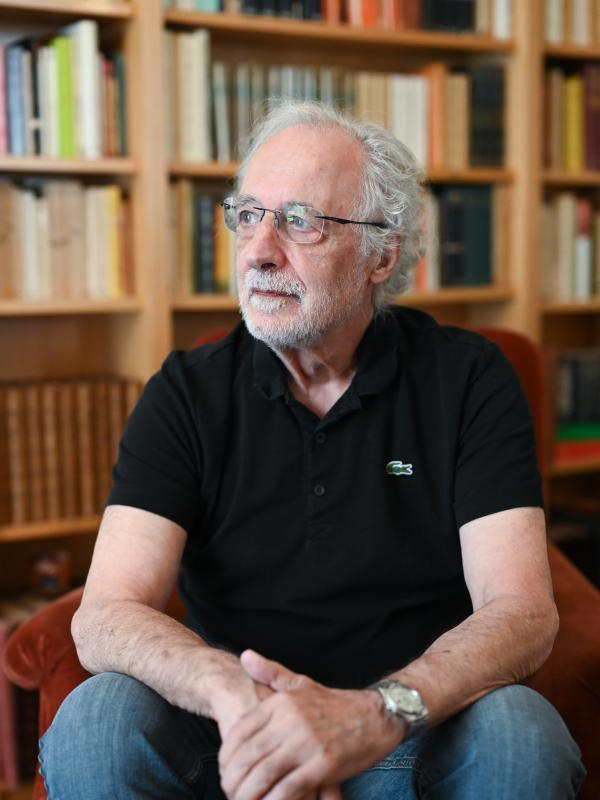
\includegraphics[width= 1\linewidth]{8}
		\caption{\small\textit{\color{timhieukhoahoc}Pierre Agostini, ảnh tại trang web khoa Vật lý, Đại học Bang Ohio.}}
		\vspace*{-10pt}
	\end{figure}
	\textbf{\color{timhieukhoahoc}Electron trong xung ánh sáng}
	\vskip 0.1cm
	Qua các thí nghiệm của mình, ba nhà khoa học được giải năm nay đã tạo được những chớp sáng đủ ngắn để chụp được chuyển động vô cùng nhanh của electron. Anne L'Huillier phát hiện ra một hiệu ứng mới từ tương tác của ánh sáng laser với các nguyên tử khí. Pierre Agostini và Ferenc Krausz cho thấy hiệu ứng này có thể được dùng để tạo ra những xung ánh sáng ngắn hơn những cái có thể được tạo ra trước đó.
	\vskip 0.1cm
	Một con chim ruồi có thể đập cánh $80$ lần mỗi giây. Chúng ta chỉ có thể nhận thấy tiếng vù vù và chuyển động mờ mờ. Với giác quan của con người, chuyển động nhanh bị mờ vào với nhau, và những sự kiện cực ngắn là không thể quan sát. Chúng ta cần đến những biện pháp công nghệ để chụp hoặc mô tả được những khoảnh khắc rất ngắn đó.
	\vskip 0.1cm
	Kỹ thuật chụp ảnh tốc độ cao và ánh sáng nhấp nháy cho phép chụp được hình ảnh chi tiết của những hiện tượng thoáng qua. Một bức ảnh rõ nét chụp một con chim ruồi đang bay đòi hỏi thời gian phơi sáng ngắn hơn nhiều so với một nhịp đập cánh của nó.
	\vskip 0.1cm
	Sự kiện càng nhanh, thời gian chụp ảnh phải càng ngắn để chụp được đúng khoảnh khắc.
	\vskip 0.1cm
	Nguyên lý tương tự được áp dụng cho tất cả các phương pháp để đo hoặc mô tả các quá trình nhanh; mọi phép đo phải được thực hiện nhanh hơn khoảng thời gian để hệ thống được quan sát trải qua một thay đổi nhận biết được, bằng không kết quả sẽ không rõ. Các nhà khoa học được giải năm nay đã tiến hành các thí nghiệm chỉ ra một phương pháp tạo ra các xung ánh sáng đủ ngắn để chụp được hình ảnh về các quá trình bên trong nguyên tử và phân tử.
	\vskip 0.1cm
	Thang thời gian tự nhiên của nguyên tử là cực kỳ nhỏ. Trong một phân tử, các nguyên tử có thể di chuyển và quay trong một phần triệu tỷ giây, hay femto giây\footnote[5]{\color{timhieukhoahoc}$1$ femto giây $= 10^{-15}$ giây -- Pi.} . Những chuyển động này có thể được nghiên cứu với những xung ngắn nhất mà một tia laser có thể tạo ra -- tuy nhiên, khi cả nguyên tử di chuyển, thang thời gian được xác định bởi hạt nhân to và nặng, vốn cực kỳ chậm so với ánh sáng và các electron nhanh nhẹn.
	\vskip 0.1cm
	Khi electron di chuyển trong nguyên tử và phân tử, chúng nhanh đến nỗi các thay đổi bị mờ sau chỉ một femto giây. Trong thế giới của electron, vị trí và năng lượng thay đổi với tốc độ từ khoảng một đến một vài trăm atto giây, tức một phần tỷ tỷ giây.
	\vskip 0.1cm
	Một atto giây ngắn đến nỗi số atto giây trong một giây bằng số giây từ khi vũ trụ sinh ra, $13{,}8$ tỷ năm trước, đến hiện tại. Để dễ hình dung, ta có thể tưởng tượng một chớp sáng đi từ một đầu căn phòng đến bức tường đối diện: nó mất mười tỷ atto giây.
	\vskip 0.1cm
	Trong một thời gian dài, một femto giây được coi là giới hạn của những chớp sáng tạo ra được.
	\vskip 0.1cm
	Việc cải tiến công nghệ sẵn có không đủ để thấy được các quá trình diễn ra trong thang thời gian ngắn đến kinh ngạc của electron; cần có một cái gì đó hoàn toàn mới. Các nhà khoa học được giải năm nay đã thực hiện những thí nghiệm mở ra lĩnh vực vật lý atto giây mới mẻ.
	\vskip 0.1cm
	\textbf{\color{timhieukhoahoc}Xung ngắn hơn nhờ các sóng hài bậc cao}
	\vskip 0.1cm
	Ánh sáng gồm những sóng -- dao động trong trường điện từ -- di chuyển trong chân không nhanh hơn mọi thứ. Sóng ánh sáng có các bước sóng khác nhau, tương đương với màu sắc khác nhau. Thí dụ, bước sóng của ánh sáng đỏ dài khoảng $700$ nm, tức khoảng một phần trăm bề rộng của một sợi tóc, và nó lặp đi lặp lại khoảng bốn trăm ba mươi nghìn tỷ lần mỗi giây. Chúng ta có thể nghĩ về xung ánh sáng ngắn nhất có thể như độ dài một chu kỳ của sóng ánh sáng, tính từ khi nó ở trên đỉnh, đi xuống đáy, rồi quay lại điểm bắt đầu. Trong trường hợp này, bước sóng dùng trong một hệ laser thông thường không thể nào đạt dưới femto giây, vì vậy trong những năm $1980$, đây được xem là một giới hạn cứng cho độ ngắn của một xung ánh sáng.
	\vskip 0.1cm
	Về mặt toán học, có thể chứng minh được rằng có thể tạo được mọi dạng sóng nếu có đủ những sóng có bước sóng và biên độ thích hợp. Bí quyết tạo ra xung atto giây là có thể tạo ra những xung ngày càng ngắn bằng cách kết hợp các bước sóng ngày càng ngắn.
	\vskip 0.1cm
	Để quan sát chuyển động của electron ở thang nguyên tử, cần các xung ánh sáng đủ ngắn, nghĩa là cần kết hợp nhiều sóng ngắn với bước sóng khác nhau.
	\vskip 0.1cm
	Để thêm bước sóng mới cho ánh sáng, cần nhiều hơn là một laser; chìa khóa dẫn đến khoảnh khắc ngắn nhất quan sát được từ trước đến nay là một hiện tượng xảy ra khi laser đi qua một chất khí. Ánh sáng tương tác với các nguyên tử khí và gây ra sóng hài bậc cao -- những sóng hoàn thành nhiều chu kỳ tương ứng với mỗi chu kỳ của sóng ban đầu. Chúng ta có thể so sánh hiện tượng này với âm bội tạo ra đặc tính của một âm thanh, giúp ta nghe được sự khác biệt của cùng một nốt khi được chơi trên ghi--ta và khi được chơi trên pi--a--nô.
	\vskip 0.1cm
	Năm $1987$, Anne L'Huillier và các đồng nghiệp tại một phòng thí nghiệm ở Pháp đã tạo được sóng hài bậc cao bằng cách sử dụng một laser hồng ngoại chiếu qua một khí hiếm. Laser hồng ngoại này tạo ra các sóng hài bậc cao ngày càng mạnh hơn so với những laser bước sóng ngắn được dùng trong các thí nghiệm trước đó. Trong thí nghiệm này, họ đã quan sát được nhiều sóng hài bậc cao với cường độ tương tự nhau.
	\vskip 0.1cm
	Trong một loạt các bài báo trong những năm $1990$, L'Huillier tiếp tục tìm hiểu hiệu ứng này, cả khi bà đã chuyển đến Đại học Lund. Những kết quả của bà đóng góp cho hiểu biết lý thuyết về hiện tượng này, đặt nền móng cho thí nghiệm đột phá tiếp theo.
	\vskip 0.1cm
	\textbf{\color{timhieukhoahoc}Electron thoát ly tạo sóng hài bậc cao}
	\vskip 0.1cm
	Khi ánh sáng laser đi qua chất khí và tác động lên các nguyên tử khí, nó tạo ra những dao động điện từ làm biến dạng điện trường giữ các electron quanh hạt nhân nguyên tử. Do đó, electron có thể thoát khỏi nguyên tử. Tuy nhiên, điện trường của ánh sáng dao động liên tục và khi nó đổi hướng, một electron đã thoát ra có thể chạy ngược về hạt nhân nguyên tử của nó. Trong chuyến du hành của mình, electron nhận thêm nhiều năng lượng từ điện trường của ánh sáng laser, và để liên kết lại với hạt nhân, nó cần giải phóng năng lượng dư thừa dưới dạng xung ánh sáng. Những xung phát ra từ electron này chính là thứ tạo ra sóng hài bậc cao được quan sát trong thí nghiệm.
	\vskip 0.1cm
	Năng lượng của ánh sáng gắn liền với bước sóng của nó. Năng lượng trong sóng hài bậc cao được phát ra tương đương với ánh sáng cực tím, vốn có bước sóng ngắn hơn ánh sáng nhìn thấy bằng mắt thường. Vì năng lượng đến từ dao động của laser, dao động của sóng hài bậc cao tỷ lệ một cách đẹp đẽ với bước sóng của xung laser ban đầu. Tương tác của ánh sáng với nhiều nguyên tử khác nhau cho kết quả là nhiều sóng ánh sáng khác nhau với những bộ bước sóng riêng.
	\vskip 0.1cm
	Khi đã được tạo ra, những sóng hài bậc cao này tương tác với nhau. Ánh sáng mạnh hơn khi các đỉnh sóng trùng nhau, và yếu hơn khi đỉnh của sóng này trùng với đáy của sóng khác. Trong những điều kiện thích hợp, các sóng hài bậc cao trùng khít với nhau, tạo ra một chuỗi các xung cực tím, mỗi xung dài vài trăm atto giây. Các nhà vật lý hiểu được lý thuyết đằng sau hiện tượng này từ những năm $1990$, nhưng đột phá trong việc xác định và kiểm nghiệm các xung này đến vào năm $2001$.
	\begin{figure}[H]
		\vspace*{-5pt}
		\centering
		\captionsetup{labelformat= empty, justification=centering}
		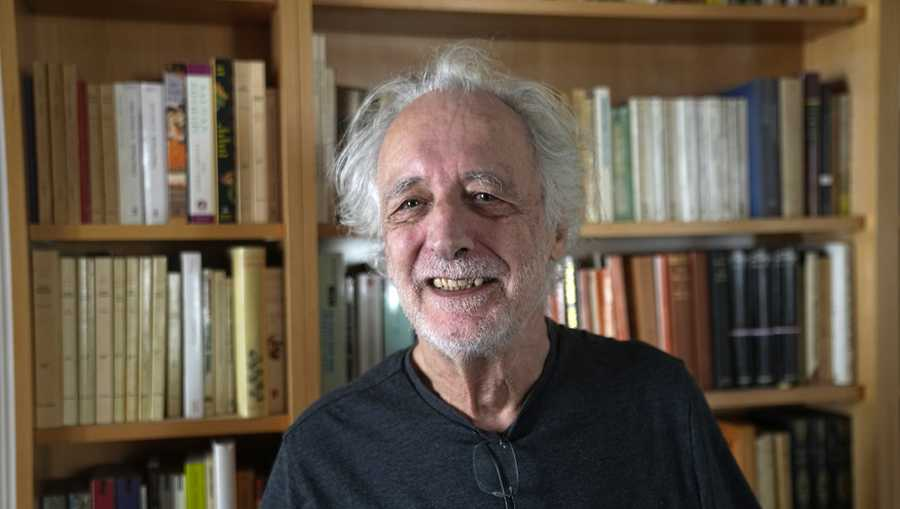
\includegraphics[width= 1\linewidth]{10}
		\caption{\small\textit{\color{timhieukhoahoc}Nhà vật lý Pháp  Pierre Agostini.}}
		\vspace*{-10pt}
	\end{figure}
	Pierre Agostini và nhóm nghiên cứu của ông tại Pháp đã thành công trong việc tạo ra và nghiên cứu một chuỗi các xung ánh sáng liên tiếp, như một đoàn tàu có nhiều toa. Họ sử dụng một kỹ thuật đặc biệt, đặt ``đoàn tàu xung" cùng với một phần bị lùi lại của xung laser ban đầu, để thấy được cách các sóng hài bậc cao đồng pha với nhau. Quá trình này cũng cho phép họ đo độ dài của các xung trong đoàn tàu, và họ nhận thấy mỗi xung chỉ dài $250$ atto giây.
	\vskip 0.1cm
	Cùng lúc đó, Ferenc Krausz và nhóm nghiên cứu của mình tại Áo đang nghiên cứu một kỹ thuật để chọn ra một xung riêng lẻ, như một toa được tách khỏi đoàn tàu và đặt sang một đường ray khác. Xung mà họ tách thành công dài $650$ atto giây và nhóm dùng nó để theo dõi và nghiên cứu một quá trình trong đó electron bị kéo ra khỏi nguyên tử.
	\vskip 0.1cm
	Những thí nghiệm này cho thấy các xung atto giây có thể được quan sát và đo, và chúng cũng có thể được sử dụng trong những thí nghiệm mới.
	\vskip 0.1cm
	Giờ thì thế giới atto giây đã mở ra, những xung ánh sáng ngắn này có thể được dùng để nghiên cứu chuyển động của electron. Hiện nay, người ta đã có thể tạo ra các xung chỉ dài vài chục atto giây, và những kỹ thuật này vẫn liên tục phát triển.
	\vskip 0.1cm
	\textbf{\color{timhieukhoahoc}Tiếp cận với chuyển động của electron}
	\vskip 0.1cm
	Các xung atto giây cho phép đo khoảng thời gian để kéo một electron khỏi nguyên tử, và xem xét sự phụ thuộc của khoảng thời gian này vào độ chặt chẽ của liên kết giữa electron với hạt nhân nguyên tử của nó. Ngày nay, có thể xây dựng lại cách mà phân bố electron dao động từ bên này sang bên kia hoặc từ nơi này đến nơi khác trong phân tử và vật chất; trước đây vị trí của chúng chỉ có thể được đo bằng một giá trị trung bình.
	\vskip 0.1cm
	Xung atto giây có thể được dùng để kiểm tra các quá trình nội tại của vật chất, và để nhận dạng các sự kiện khác nhau. Những xung này đã được dùng để tìm hiểu vật lý chi tiết của nguyên tử và phân tử, và chúng có những ứng dụng tiềm năng trong nhiều lĩnh vực, từ điện tử đến y học.
	\vskip 0.1cm
	Chẳng hạn, xung atto giây có thể được dùng để đẩy các phân tử, khiến chúng phát ra những tín hiệu đo được. Tín hiệu phát ra từ các phân tử có cấu trúc đặc biệt, một dạng ``vân tay" giúp nhận dạng phân tử, điều này có những ứng dụng tiềm năng, bao gồm chẩn đoán y tế.
\end{multicols}
	\newpage

	\thispagestyle{empty}
	\begingroup 
	\AddToShipoutPicture*{\put(0,0){\includegraphics[width=19.5cm]{MV.pdf}}}
	\centering
	\vspace*{0cm}
	\endgroup
	\newpage	
	\pagestyle{empty}

	\setcounter{figure}{0}
	\thispagestyle{quantoannone}
\pagestyle{quantoan}
\everymath{\color{quantoan}}
\graphicspath{{../quantoan/pic/}}
\blfootnote{\color{quantoan}\color{quantoan}$^*$Theo The Economist.}
\blfootnote{\color{quantoan}\color{quantoan}$^1$Đại học Sư phạm Hà Nội.}
\begingroup
\AddToShipoutPicture*{\put(0,616){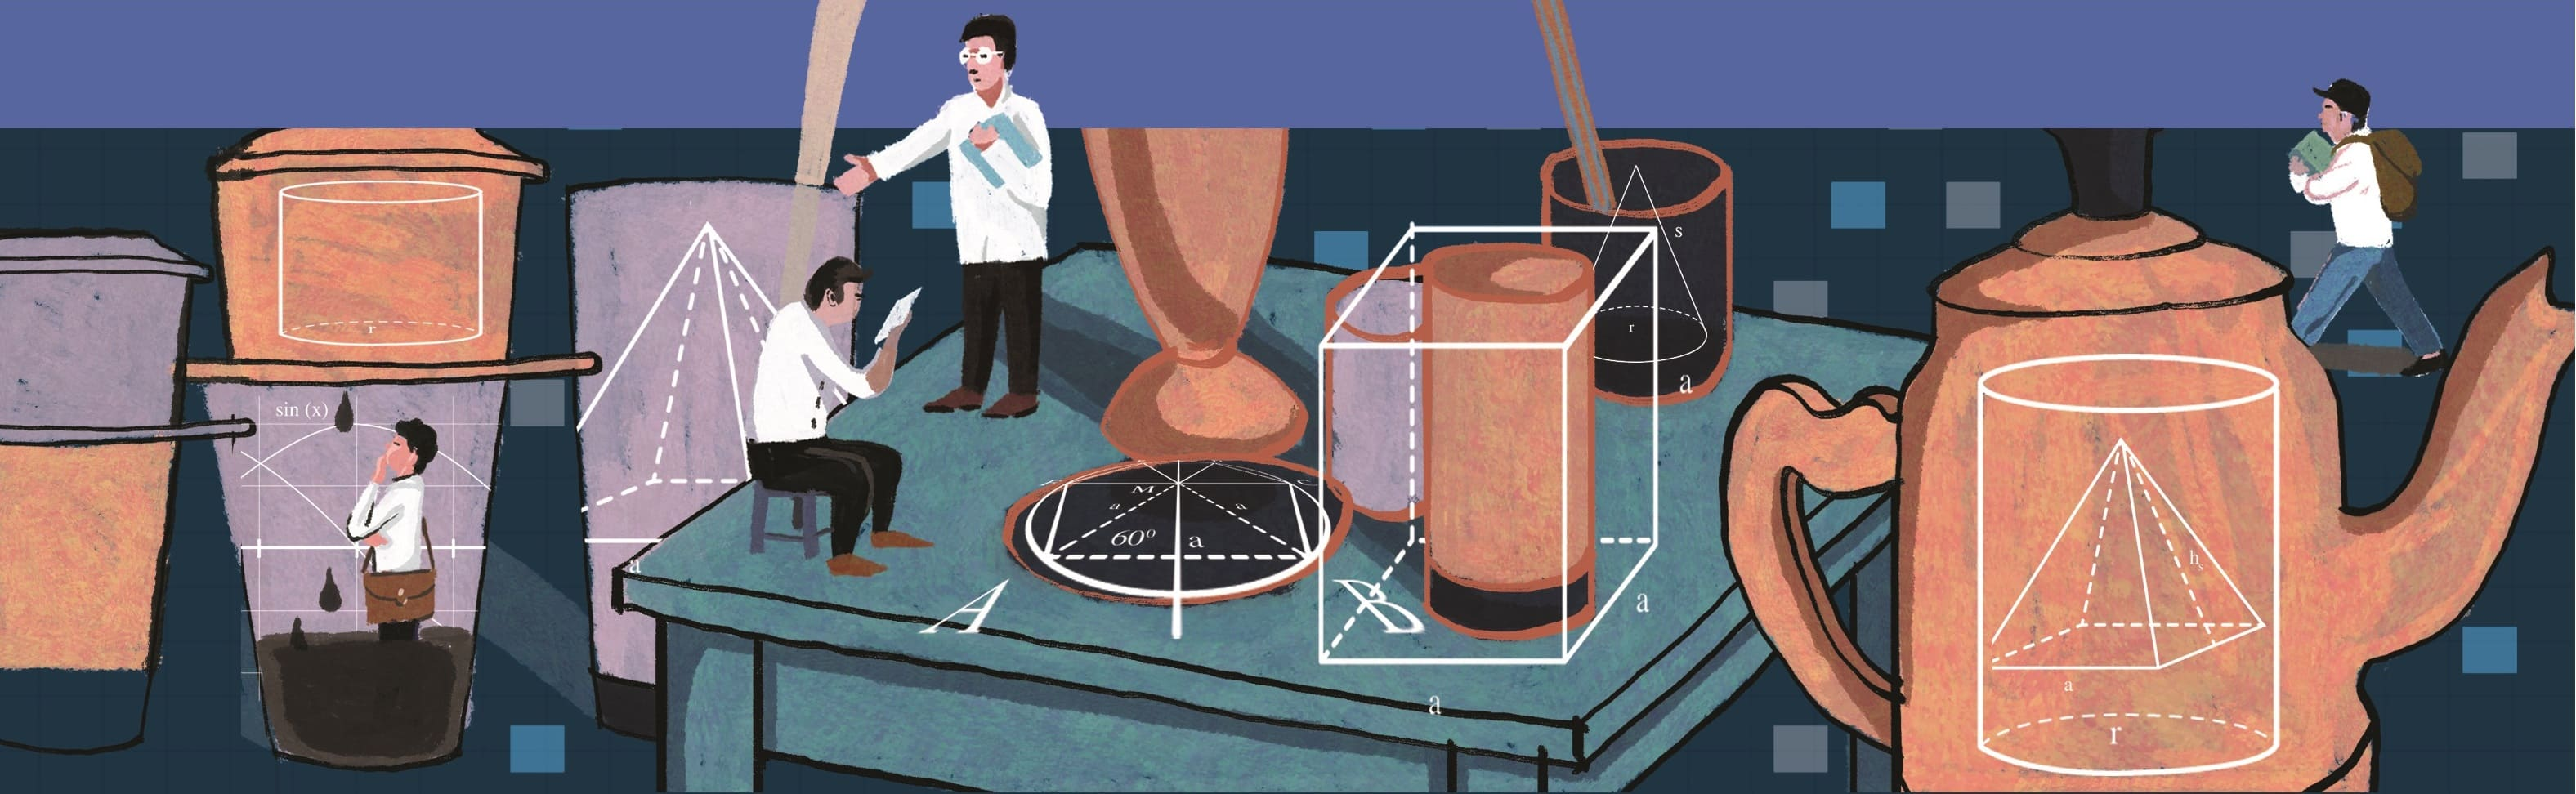
\includegraphics[width=19.3cm]{../bannerquantoan}}}
\AddToShipoutPicture*{\put(126,520){
\includegraphics[scale=1]{../tieude3.pdf}}}
\centering
\endgroup

\vspace*{180pt}

\begin{multicols}{2}
	Có một truyền thuyết  kể rằng thành phố Portland, bang Oregon đã suýt được gọi là Boston. Cuối cùng thì vấn đề đã được quyết định nhờ một cuộc tung đồng xu được tổ chức vào năm $1845$ giữa Francis Pettygrove, người đến từ một thành phố Portland khác, ở bang Maine, và Asa Lovejoy, đến từ Boston (ở bang Massachusetts). Nhưng mọi chuyện có thể đã khác đi, theo Frantisek Bartos, một sinh viên tốt nghiệp tại Đại học Amsterdam, nếu con người chúng ta  không phải là những người tung xu một cách lưỡng lự thiếu dứt khoát như vậy.
	\begin{figure}[H]
		\vspace*{-5pt}
		\centering
		\captionsetup{labelformat= empty, justification=centering}
		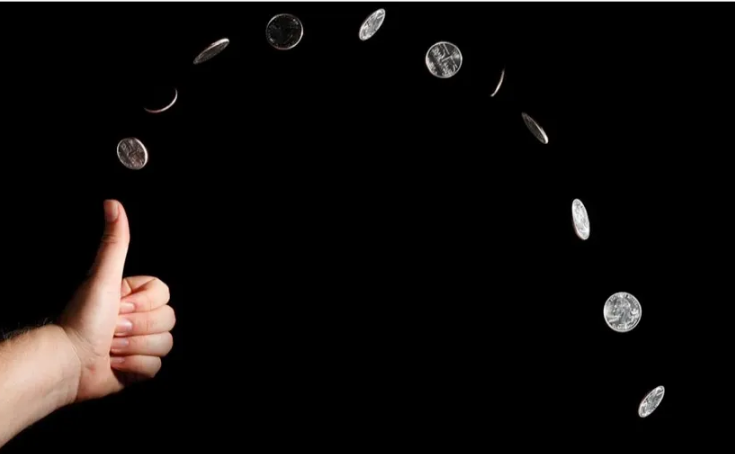
\includegraphics[width= 1\linewidth]{1111}
%		\caption{\small\textit{\color{}}}
		\vspace*{-15pt}
	\end{figure}
	Bartos đã quan tâm đến một dự đoán hấp dẫn của Persi Diaconis, Susan Holmes và Richard Montgomery, một nhóm các nhà toán học người Mỹ. Trong một bài báo đăng vào năm $2007$, bộ ba này đã phân tích tính chất vật lý của việc tung đồng xu và nhận thấy có một điều gì đó khá hấp dẫn. Bên cạnh việc khiến đồng xu quay lộn nhào, hầu hết mọi người đều có xu hướng tạo ra một sự xoay nhẹ cho đồng xu khi họ tung nó. Điều đó làm cho trục xuay mà đồng xu lật quanh đó sẽ bị trôi đẩy khi nó ở trên không trung, một hiện tượng gọi là tuế sai.
	\vskip 0.01cm
	Kết quả cuối cùng, khi các con số được xử lý, là: một đồng xu do con người ném sẽ thể hiện một xu hướng thiên lệch khá tinh tế nhưng bền vững. Tiến sĩ Diaconis và các đồng nghiệp của ông tính toán có khoảng $51\%$ khả năng một đồng xu sẽ rơi theo hướng như trước khi được ném. Nói cách khác, nếu nó ngửa trong tay người ném, có nhiều khả năng hơn một chút là nó cũng sẽ chạm đất ngửa. Hoặc ít nhất, đó cũng là dự đoán.
	\vskip 0.01cm
	Bartos cùng với sự nhiệt tình đáng ngưỡng mộ của mình bắt tay vào kiểm tra thực nghiệm. Anh đã tập hợp được $48$ tình nguyện viên và thuyết phục họ thực hiện (và có quay phim) $350{.}707$ lần tung đồng xu, sử dụng hàng chục đồng xu khác nhau, từ đồng hai rupee của Ấn Độ đến đồng xu hai franc Thụy Sỹ. Dĩ nhiên, dữ liệu của anh  đã xác nhận những gì vật lý đã dự đoán. Các đồng xu đã chạm đất cùng với mặt khi tung lên tới tận $50,8\%$ số lần được ném.
	\vskip 0.01cm
	Số liệu thống kê chỉ ra rằng bản thân các đồng xu không có sự thiên lệch cụ thể nào. Yếu tố quyết định thực sự là con người chúng ta rõ ràng không có khả năng ném thẳng.  Bartos không phải là người đầu tiên thu thập số liệu thống kê về việc tung đồng xu. Nhưng anh ta là người đầu tiên làm được điều đó ở quy mô đủ lớn để phát hiện ra sự thiên lệch. (Một nỗ lực trước đó gồm $40{.}000$ lần tung, do hai sinh viên tại Đại học California tại Berkeley  thực hiện, đã thiếu sức mạnh thống kê để xác nhận được  lý thuyết.)
	\vskip 0.1cm
	Cơ hội $50,8\%$ chỉ khác một chút so với mức công bằng hoàn hảo. Nhưng  Bartos chỉ ra rằng cơ hội đó lớn hơn cả  lợi thế mà một sòng bạc có được trong hầu hết các loại kiểu chơi blackjack. Và trong một số tình huống cơ hội đó có thể có vai trò quan trọng. Vào năm $2019$, Sue Cudilla trở thành thị trưởng của Araceli, một thị trấn ở Philippines, nhờ việc tung đồng xu sau khi cuộc bầu cử được tuyên bố là bất phân thắng bại. Quan trọng hơn nữa, việc tung đồng xu có thể xác định ai là người ném bóng hoặc đánh bóng trước trong môn cricket. Các vận động viên chuyên nghiệp luôn chi hàng nghìn đô--la  và hàng giờ tập luyện để tìm kiếm được những lợi thế cận biên. Có lẽ họ giờ  sẽ phải nên chú ý nhìn vào đồng xu lẻ trong túi quần của trọng tài.
\end{multicols}
\vspace*{-10pt}
{\color{quantoan}\rule{1\linewidth}{0.1pt}}
\blfootnote{\color{quantoan}\color{quantoan}$^*$Bài nói tại Viện hàn lâm Leopoldina của Berlin.}
\blfootnote{\color{quantoan}\color{quantoan}$^1$Freie Universität, Berlin.  Xem thêm bài phỏng vấn ở Pi số $3$, năm $2022$}
\begingroup
\AddToShipoutPicture*{\put(88,385){
\includegraphics[scale=1]{../tieude.pdf}}}
\centering
\endgroup

\vspace*{75pt}

\begin{multicols}{2}
	\textbf{\color{quantoan}Một lựa chọn nhỏ các trích dẫn}
	\vskip 0.1cm
	\textit{Wolfgang Goethe: Các nhà toán học là một kiểu người Pháp: nếu bạn nói chuyện với họ, họ sẽ dịch nó sang ngôn ngữ của họ, và sau đó nó sẽ sớm trở thành một thứ gì đó hoàn toàn khác. Goethe thực sự không thích tiếng Pháp cũng như các nhà toán học (!) vì ông đã viết: Nền văn hóa mà toán học mang lại cho trí tuệ là vô cùng phiến diện và hạn chế.
		\vskip 0.1cm
		Leonardo da Vinci: Bất cứ ai chỉ trích trí tuệ siêu phàm của toán học đều nuôi dưỡng sự nhầm lẫn.
		\vskip 0.1cm
		Cess Noteboom: Vì nghề nghiệp của mình, tôi đã quen với một số kiểu hoàn hảo nhất định. Một trong số đó là toán học. Toán học, nếu bạn tìm hiểu sâu hơn, có hình mái vòm của thơ ca, trong đó không có những điều không thể dự đoán trước, và nếu chúng ta thành thật mà nói, thì không có cả sự lầy lội của con người.  
		Albert Einstein: Toán học thuần túy, theo cách riêng của nó, là thi ca của những suy nghĩ logic.
		\begin{figure}[H]
			\vspace*{-5pt}
			\centering
			\captionsetup{labelformat= empty, justification=centering}
			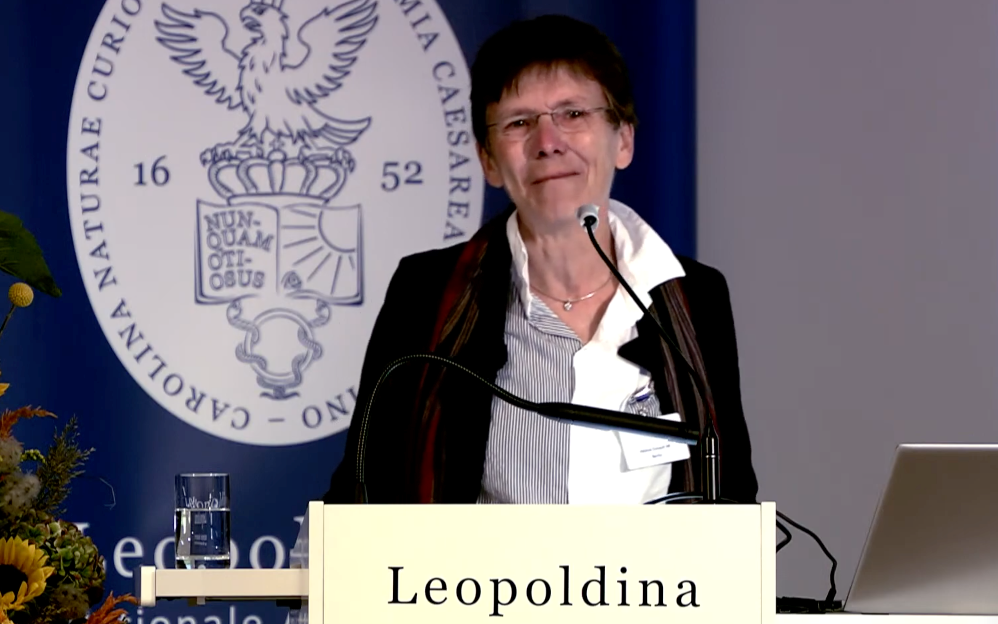
\includegraphics[width= 1\linewidth]{1aa}
			%		\caption{\small\textit{\color{}}}
			\vspace*{-15pt}
		\end{figure}
		Karl Weierstrass: Đúng là một nhà toán học không có chút gì là thơ sẽ không bao giờ là một nhà toán học hoàn hảo.}
	\vskip 0.1cm
	\textbf{\color{quantoan}Tại sao chúng tôi làm toán?}
	\vskip 0.1cm
	Những con đường dẫn đến toán học có lẽ cũng nhiều như số người theo đuổi nó. Nhưng có một điều không đổi: toán học là tự do của chúng tôi. Một số người đến với toán học thông qua vật lý, một số người thông qua khoa học máy tính, một số người  thông qua kỹ thuật, một số người thông qua sinh học. Sẽ có lúc trong đời sống trí tuệ ta muốn sắp xếp lại những suy nghĩ của mình trước khi áp dụng chúng, hay khi ta muốn hiểu được nền tảng của chúng. Đó là sự hấp dẫn của sự trừu tượng, dù nó thường xa rời thực tế của thế giới bên ngoài.
	\vskip 0.1cm
	Những người khác đến với toán học thông qua nghệ thuật, thơ ca, triết học. Sẽ có thời điểm ta cố gắng vượt qua sự chủ quan trong thẩm mỹ. Đó là lúc ta cần tiêu chí ``đúng hoặc sai" của tựa đề bài viết. Chúng tôi phân biệt hai động cơ: ``trừu tượng" và ``đúng hoặc~sai".
	\vskip 0.1cm
	\textbf{\color{quantoan}Chúng tôi thực sự làm gì?}
	\vskip 0.1cm
	Chúng tôi thường bắt đầu khá trẻ. Với tôi, thời trẻ tôi đã bị lôi cuốn bởi sự trừu tượng, bao gồm cả điều ``đúng hoặc sai" này. Toán học buộc bạn phải suy nghĩ với những lập luận được xây dựng rõ ràng. Đó là một sự bảo vệ khỏi chủ nghĩa giáo điều. Toán học có thể cứu chúng ta khỏi sự thờ ơ với xã hội, xóa bỏ nỗi sợ hãi về tương lai và giải phóng chúng ta khỏi kỳ vọng mình sẽ có ích trong xã hội. Tất nhiên, toán học được xã hội hoan nghênh vì nó có ứng dụng, lấy ví dụ ChatGPT. 
	\vskip 0.1cm
	Nhiều người trong chúng ta cũng nỗ lực để lao động của họ có ứng dụng trong xã hội. Nhưng những người khác, trong đó có tôi, thì không. Tôi lớn lên dưới ảnh hưởng của Hiroshima và không bao giờ muốn làm bất cứ điều gì trong đời mà có thể gây ra hậu quả tàn khốc. Đó là lý do tại sao tôi quyết định nghiên cứu một thứ không mang lại kết quả gì cả: nghiên cứu trong ``lĩnh vực trừu tượng nhất" của toán học. Khi tôi nghĩ về toán học, thực tế của thế giới bên ngoài biến mất. Toán học hoạt động với các khái niệm khép kín. Một lý thuyết toán học dựa trên những ý tưởng phải tương thích với hàng nghìn ý tưởng đã được thêm vào cấu trúc toán học trước đó. Mỗi lý thuyết được ghi lại bằng một ngôn ngữ đặc biệt, thể hiện thông qua các định lý, mệnh đề, bổ đề, tất cả đều thuộc về các quy tắc chung của toán học và lý thuyết này được hỗ trợ bởi các chứng minh. 
	\vskip 0.1cm
	Điều bạn nhận được luôn là ``đúng" hoặc ``sai". Sai có thể là một lỗi logic, hoặc có thể được phát hiện từ sự không tương thích với một lý thuyết trước đó. Trong trường hợp sau, cũng có thể lý thuyết trước đó là sai. Đôi khi bạn tìm thấy lỗi trong những bài viết đã hơn $100$ năm tuổi. Trong hầu hết các trường hợp, lỗi được phát hiện quá muộn là do lý thuyết cũ không còn quan trọng cho sự phát triển tiếp theo. Chúng tôi làm việc với những bài toán. Trong sự trừu tượng này, bản thân các bài toán đều xuất phát từ những suy nghĩ trừu tượng. Mỗi bước hiểu biết đều mang tới những bài toán mới, nó cứ tiếp diễn mãi. Các bài toán trong các lĩnh vực toán học thiên về ứng dụng hơn có thể đến từ toán học bên ngoài, nghĩa là, từ ``thực tế"...
	\vskip 0.1cm
	\textbf{\color{quantoan}Tại sao chúng tôi không cảm thấy mệt mỏi?}
	\vskip 0.1cm
	Một người bạn đã hỏi tôi như vậy gần đây. Tôi có hai ý để trả lời câu hỏi này. Một mặt, khi ta hiểu được một điều gì đó, dù nó rất nhỏ, thì niềm vui cũng vô cùng lớn lao, không gì có thể so sánh được. Không ai có thể tước đoạt điều đó từ ta. Thứ hai, chúng tôi muốn biết. Chúng tôi thực sự muốn biết. Tôi đã nói rằng, với tư cách là một nhà toán học tôi gặp khó khăn với một khái niệm trừu tượng của thực tế. Nhưng nếu bạn hỏi với tôi, hay nhiều người trong chúng tôi, thực tế chủ quan là gì, thì tôi sẽ trả lời: Mong muốn biết vô điều kiện. 
\end{multicols}

	\newpage

	\thispagestyle{empty}
	\begingroup 
	\AddToShipoutPicture*{\put(0,0){\includegraphics[width=19.45cm]{QC}}}
	\centering
	\vspace*{0cm}
	\endgroup
	\newpage	 
	\pagestyle{empty}

	\setcounter{figure}{0}
	\thispagestyle{toancuabinone}
\pagestyle{toancuabi}
\everymath{\color{toancuabi}}
\blfootnote{$^*$\color{toancuabi}Nguồn: Câu lạc bộ Toán học Unicorn (UMC)}
\graphicspath{{../toancuabi/pic/}}
\begingroup
\AddToShipoutPicture*{\put(0,616){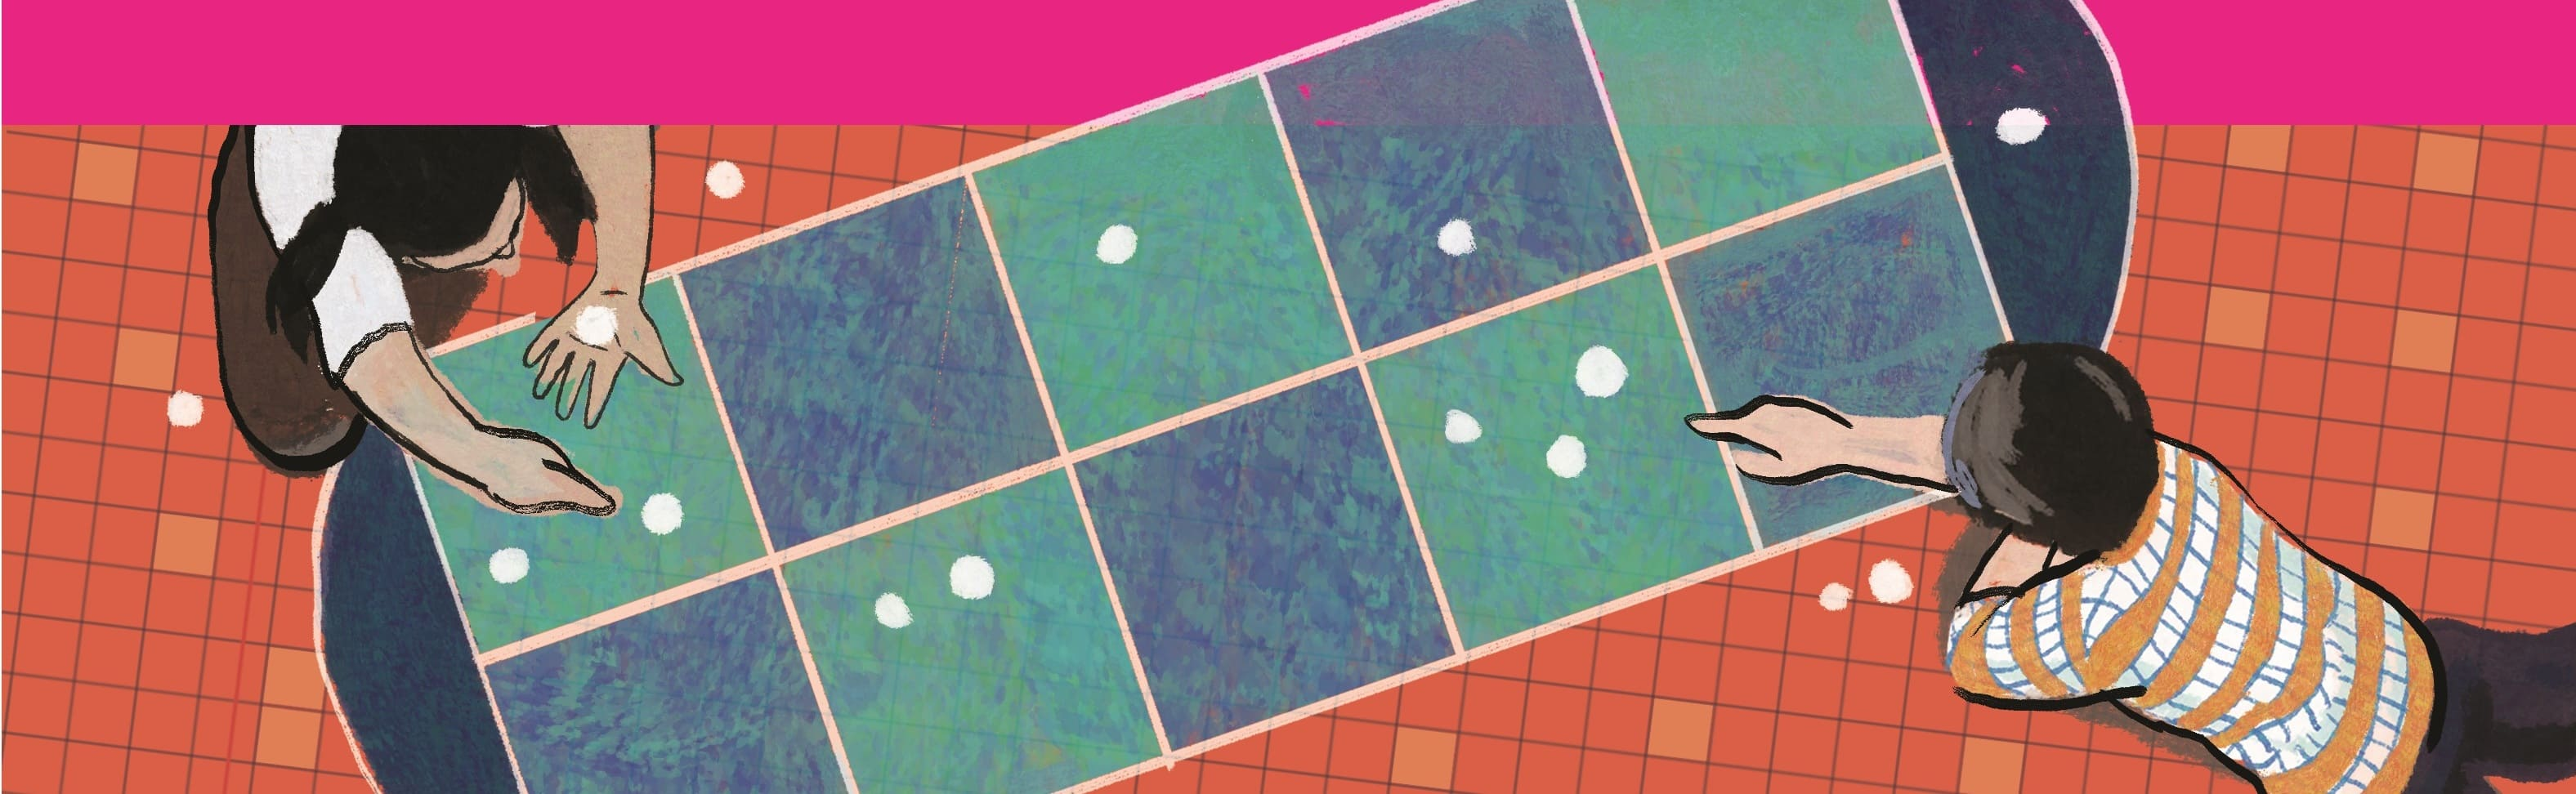
\includegraphics[width=19.3cm]{../bannertoancuabi}}}  
\AddToShipoutPicture*{\put(62,512){
\includegraphics[scale=1]{../tieude1.pdf}}}  
\centering
\endgroup
\vspace*{195pt} 

\definecolor{bulgarianrose}{rgb}{0.28, 0.02, 0.03}
\begin{multicols}{2}
	Trong số này, tạp chí Pi tiếp tục giới thiệu đến với bạn đọc đề thi tuyển sinh năm $2023-2024$ dành cho các bạn học sinh lớp $5$. Các bạn có thể thử sức làm của mình trong khoảng thời gian $90$ phút.
	\vskip 0.1cm
	\textbf{\color{toancuabi}Bài $\pmb1$.} 
	Dựa vào quy luật, hãy cho biết có bao nhiêu dấu thăng trong hình thứ tám của dãy hình sau.
	\begin{figure}[H]
		\vspace*{-5pt}
		\centering
		\captionsetup{labelformat= empty, justification=centering}
		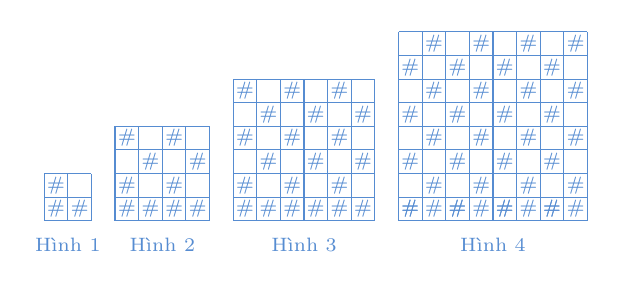
\begin{tikzpicture}[cackithi,scale=0.3,node font=\scriptsize]
			\draw (0,0) grid (2,2);	
			\draw (3,0) grid (7,4);
			\draw (8,0) grid (14,6);
			\draw (15,0) grid (23,8);
			\draw (0.5,0.5) node {$\#$};
			\draw (1.5,0.5) node {$\#$};
			\draw (0.5,1.5) node {$\#$};
			\draw (3.5,0.5) node {$\#$};
			\draw (4.5,0.5) node {$\#$};
			\draw (5.5,0.5) node {$\#$};
			\draw (6.5,0.5) node {$\#$};
			\draw (3.5,1.5) node {$\#$};
			\draw (5.5,1.5) node {$\#$};
			\draw (4.5,2.5) node {$\#$};
			\draw (6.5,2.5) node {$\#$};
			\draw (3.5,3.5) node {$\#$};
			\draw (5.5,3.5) node {$\#$};
			\draw (8.5,0.5) node {$\#$};
			\draw (9.5,0.5) node {$\#$};
			\draw (10.5,0.5) node {$\#$};
			\draw (11.5,0.5) node {$\#$};
			\draw (12.5,0.5) node {$\#$};
			\draw (13.5,0.5) node {$\#$};
			\draw (8.5,1.5) node {$\#$};
			\draw (10.5,1.5) node {$\#$};
			\draw (12.5,1.5) node {$\#$};
			\draw (9.5,2.5) node {$\#$};
			\draw (11.5,2.5) node {$\#$};
			\draw (13.5,2.5) node {$\#$};
			\draw (8.5,3.5) node {$\#$};
			\draw (10.5,3.5) node {$\#$};
			\draw (12.5,3.5) node {$\#$};
			\draw (9.5,4.5) node {$\#$};
			\draw (11.5,4.5) node {$\#$};
			\draw (13.5,4.5) node {$\#$};
			\draw (8.5,5.5) node {$\#$};
			\draw (10.5,5.5) node {$\#$};
			\draw (12.5,5.5) node {$\#$};
			\draw (15.5,0.5) node {$\#$};
			\draw (16.5,0.5) node {$\#$};
			\draw (17.5,0.5) node {$\#$};
			\draw (18.5,0.5) node {$\#$};
			\draw (19.5,0.5) node {$\#$};
			\draw (20.5,0.5) node {$\#$};
			\draw (21.5,0.5) node {$\#$};
			\draw (22.5,0.5) node {$\#$};
			\draw (15.5,0.5) node {$\#$};
			\draw (17.5,0.5) node {$\#$};
			\draw (19.5,0.5) node {$\#$};
			\draw (21.5,0.5) node {$\#$};
			\draw (16.5,1.5) node {$\#$};
			\draw (18.5,1.5) node {$\#$};
			\draw (20.5,1.5) node {$\#$};
			\draw (22.5,1.5) node {$\#$};
			\draw (15.5,2.5) node {$\#$};
			\draw (17.5,2.5) node {$\#$};
			\draw (19.5,2.5) node {$\#$};
			\draw (21.5,2.5) node {$\#$};
			\draw (16.5,3.5) node {$\#$};
			\draw (18.5,3.5) node {$\#$};
			\draw (20.5,3.5) node {$\#$};
			\draw (22.5,3.5) node {$\#$};
			\draw (15.5,4.5) node {$\#$};
			\draw (17.5,4.5) node {$\#$};
			\draw (19.5,4.5) node {$\#$};
			\draw (21.5,4.5) node {$\#$};
			\draw (16.5,5.5) node {$\#$};
			\draw (18.5,5.5) node {$\#$};
			\draw (20.5,5.5) node {$\#$};
			\draw (22.5,5.5) node {$\#$};
			\draw (15.5,6.5) node {$\#$};
			\draw (17.5,6.5) node {$\#$};
			\draw (19.5,6.5) node {$\#$};
			\draw (21.5,6.5) node {$\#$};
			\draw (16.5,7.5) node {$\#$};
			\draw (18.5,7.5) node {$\#$};
			\draw (20.5,7.5) node {$\#$};
			\draw (22.5,7.5) node {$\#$};
			\draw (1,-1) node {Hình $1$};
			\draw (5,-1) node {Hình $2$};
			\draw (11,-1) node {Hình $3$};
			\draw (19,-1) node {Hình $4$};
		\end{tikzpicture}
		\vspace*{-15pt}
	\end{figure}
	\textbf{\color{toancuabi}Bài $\pmb2$.} Bạn Tâm xếp các số $0, 0, 1, 1, 2, 2, 2, 3$ vào các ô vuông trong hình dưới đây (mỗi ô một số) để tạo thành phép trừ của hai số có $4$ chữ số. Hỏi hiệu nhận được lớn nhất có thể là bao nhiêu? 
	\vskip 0.1cm
	Chú ý: \textit{một số có bốn chữ số không được bắt đầu bằng số $0$.}
	\begin{figure}[H]
		\vspace*{-5pt}
		\centering
		\captionsetup{labelformat= empty, justification=centering}
		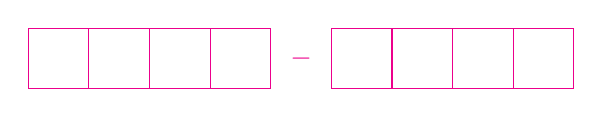
\begin{tikzpicture}[toancuabi,scale=0.77]
			\draw (0,0) grid (4,1);
			\draw (4.5,0.5) node {$-$};
			\draw (5,0) grid (9,1);
		\end{tikzpicture}
		\vspace*{-10pt}
	\end{figure}
	\textbf{\color{toancuabi}Bài $\pmb3$.} Diện tích của hình được tô đậm bên dưới bằng bao nhiêu?
	\begin{figure}[H]
		\vspace*{5pt}
		\centering
		\captionsetup{labelformat= empty, justification=centering}
		\definecolor{zzttqq}{rgb}{0.6,0.2,0.}
		\begin{tikzpicture}[toancuabi, scale=0.9]
			\fill[color=cackithi,fill=cackithi!40] (1.,0.) -- (2.,5.) -- (3.,0.) -- cycle;
			\fill[color=zzttqq,fill=cackithi!40] (1.,0.) -- (4.,5.) -- (3.,0.) -- (0.,5.) -- cycle;
			\draw  (1.,0.)-- (2.,5.);
			\draw  (2.,5.)-- (3.,0.);
			\draw  (3.,0.)-- (1.,0.);
			\draw  (1.,0.)-- (4.,5.);
			\draw  (4.,5.)-- (3.,0.);
			\draw  (3.,0.)-- (0.,5.);
			\draw  (0.,5.)-- (1.,0.);
			\draw[dashed]  (-1.,5.)-- (5.,5.);
			\draw[dashed]  (-1.,2.5)-- (5.,2.5);
			\draw[dashed]  (-1.,0.)-- (5.,0.);
			\draw[-stealth]  (4.5,5.)-- (4.5,2.5);
			\draw[-stealth]  (4.5,2.5)-- (4.5,0.);
			\draw[-stealth]  (1,-0.4)-- (3.,-0.4);
			
			\draw[-stealth]  (4.5,2.5) -- (4.5,5.);
			\draw[-stealth]  (4.5,0.) -- (4.5,2.5);
			\draw[-stealth]  (3.,-0.4) -- (1,-0.4);
			\draw[color=black] (4.21498164902576,3.87946061896495) node {$5$};
			\draw[color=black] (4.143071467449243,1.3626042637868525) node {$5$};
			\draw[color=black] (2.039698656336115,-0.709930933849792) node {$4$};
		\end{tikzpicture}
		\vspace*{-10pt}
	\end{figure}
	\textbf{\color{toancuabi}Bài $\pmb4$.} Trong bảng ô vuông cỡ $4\times 4$ có điền các số khác $0$ sao cho tích của $4$ số trong mỗi hàng, mỗi cột đều bằng nhau. Cho biết các số trong $9$ ô như hình vẽ, hỏi số ở ô có dấu $*$ bằng bao nhiêu?
	\begin{figure}[H]
		\vspace*{-5pt}
		\centering
		\captionsetup{labelformat= empty, justification=centering}
		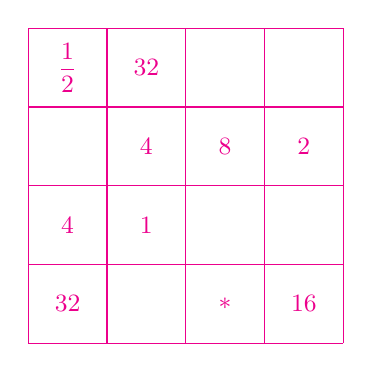
\begin{tikzpicture}[toancuabi, node font=\small]
			\draw (0,0) grid (4,4);
			\draw (0.5,0.5) node {$32$};
			\draw (0.5,1.5) node {$4$};
			\draw (0.5,3.5) node {$\dfrac{1}{2}$};
			\draw (1.5,1.5) node {$1$};
			\draw (1.5,2.5) node {$4$};
			\draw (1.5,3.5) node {$32$};
			\draw (2.5,0.5) node {$*$};
			\draw (3.5,0.5) node {$16$};
			\draw (2.5,2.5) node {$8$};
			\draw (3.5,2.5) node {$2$};
		\end{tikzpicture}
		\vspace*{-5pt}
	\end{figure}
	\textbf{\color{toancuabi}Bài $\pmb5$.} Khu vườn của gia đình Tâm được minh họa bằng hình chữ nhật trong hình dưới đây. Biết rằng khu vườn có diện tích $120 \,m^2$ và được chia thành ba luống hình chữ nhật. Phần trồng hoa rộng $2\,m$, diện tích $20 \,m^2$, phần trồng dâu rộng $3\, m$. Hỏi diện tích phần trồng rau là bao nhiêu?
	\begin{figure}[H]
		\vspace*{-5pt}
		\centering
		\captionsetup{labelformat= empty, justification=centering}
		\begin{tikzpicture}[scale=0.4,toancuabi]
			\draw (0,0) rectangle (12,10);
			\draw (2,0) -- (2,10) (2,3) -- (12,3);
			\draw (1,10) node[below] {$2\,m$};
			\draw (1,5) node {Hoa};
			\draw (7,1.5) node {Dâu};
			\draw (7,6.5) node {Rau};
			\draw (12,1.5) node[right] {$3\,m$};
		\end{tikzpicture}
		\vspace*{-5pt}
	\end{figure}
	\textbf{\color{toancuabi}Bài $\pmb6$.} Ba bạn An, Bình, Chi chia đều nhau $30$ chiếc kẹo. An ăn một số chiếc kẹo; Bình ăn một số kẹo bằng với số kẹo mà An còn; Chi ăn số kẹo bằng với tổng số kẹo mà An và Bình đã ăn. Hỏi còn lại bao nhiêu chiếc kẹo?
	\vskip 0.1cm
	\textbf{\color{toancuabi}Bài $\pmb7$.} Một bác nông dân chở một xe ô tô quất cảnh ra chợ Tết để bán. Sau khi bán hết cây quất cuối cùng với giá $230$ nghìn đồng, bác tính nhẩm lại thấy mình đã bán số cây quất với giá trung bình là $245$ nghìn đồng/cây. Nhưng người mua cây quất cuối quay trở lại và chỉ cho bác thấy cành quất bị rụng quá nhiều lá, nên ông ta chỉ đồng ý mua với giá $158$ nghìn đồng. Bác chấp thuận và bán cây quất đó. Khi nhẩm tính lại, bác nông dân thấy giá trung bình của xe quất bây giờ là $242$ nghìn đồng. Hỏi bác đã bán được bao nhiêu cây quất?
	\vskip 0.1cm
	\columnbreak
	\textbf{\color{toancuabi}Bài $\pmb8$.} Có bao nhiêu cách xếp $5$ viên bi giống hệt nhau vào các ô hình vuông ở hình vẽ sau sao cho mỗi ô có không quá $1$ viên bi và không có $2$ viên bi nào trên cùng $1$ hàng hoặc $1$ cột?
	\begin{figure}[H]
		\vspace*{-10pt}
		\centering
		\captionsetup{labelformat= empty, justification=centering}
		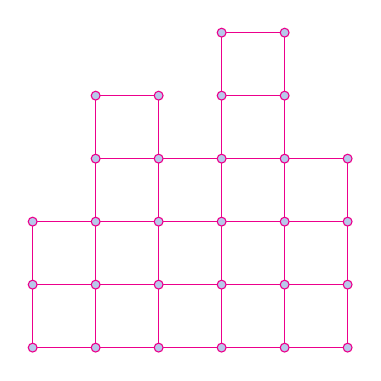
\begin{tikzpicture}[toancuabi,scale=0.8]
			\draw  (0.,1.)-- (5.,1.);
			\draw  (5.,1.)-- (5.,4.);
			\draw  (5.,4.)-- (1.,4.);
			\draw  (1.,4.)-- (1.,3.);
			\draw  (1.,3.)-- (0.,3.);
			\draw  (0.,3.)-- (0.,1.);
			\draw  (1.,1.)-- (1.,3.);
			\draw  (1.,2.)-- (5.,2.);
			\draw  (5.,3.)-- (1.,3.);
			\draw  (1.,4.)-- (1.,5.);
			\draw  (1.,5.)-- (2.,5.);
			\draw  (2.,5.)-- (2.,1.);
			\draw  (3.,1.)-- (3.,6.);
			\draw  (3.,6.)-- (4.,6.);
			\draw  (4.,6.)-- (4.,1.);
			\draw  (0.,2.)-- (1.,2.);
			\draw  (3.,5.)-- (4.,5.);
			
			\draw [fill=cackithi!40] (0.,1.) circle (2.0pt);
			\draw [fill=cackithi!40] (5.,1.) circle (2.0pt);
			\draw [fill=cackithi!40] (5.,4.) circle (2.0pt);
			\draw [fill=cackithi!40] (1.,4.) circle (2.0pt);
			\draw [fill=cackithi!40] (1.,3.) circle (2.0pt);
			\draw [fill=cackithi!40] (0.,3.) circle (2.0pt);
			\draw [fill=cackithi!40] (1.,1.) circle (2.0pt);
			\draw [fill=cackithi!40] (1.,2.) circle (2.0pt);
			\draw [fill=cackithi!40] (5.,2.) circle (2.0pt);
			\draw [fill=cackithi!40] (5.,3.) circle (2.0pt);
			\draw [fill=cackithi!40] (1.,5.) circle (2.0pt);
			\draw [fill=cackithi!40] (2.,5.) circle (2.0pt);
			\draw [fill=cackithi!40] (2.,1.) circle (2.0pt);
			\draw [fill=cackithi!40] (3.,1.) circle (2.0pt);
			\draw [fill=cackithi!40] (3.,6.) circle (2.0pt);
			\draw [fill=cackithi!40] (4.,6.) circle (2.0pt);
			\draw [fill=cackithi!40] (4.,1.) circle (2.0pt);
			\draw [fill=cackithi!40] (2.,4.) circle (2.0pt);
			\draw [fill=cackithi!40] (3.,4.) circle (2.0pt);
			\draw [fill=cackithi!40] (4.,4.) circle (2.0pt);
			\draw [fill=cackithi!40] (4.,5.) circle (2.0pt);
			\draw [fill=cackithi!40] (3.,5.) circle (2.0pt);
			\draw [fill=cackithi!40] (4.,3.) circle (2.0pt);
			\draw [fill=cackithi!40] (3.,3.) circle (2.0pt);
			\draw [fill=cackithi!40] (2.,3.) circle (2.0pt);
			\draw [fill=cackithi!40] (2.,2.) circle (2.0pt);
			\draw [fill=cackithi!40] (3.,2.) circle (2.0pt);
			\draw [fill=cackithi!40] (4.,2.) circle (2.0pt);
			\draw [fill=cackithi!40] (0.,2.) circle (2.0pt);
		\end{tikzpicture}
		\vspace*{-5pt}
	\end{figure}
	\textbf{\color{toancuabi}Bài $\pmb9$.} Mỗi ô trong hình bên được điền một số sao cho: số được ghi trong mỗi ô ở $3$ hàng trên cùng bằng tổng $2$ số ở hai ô ngay bên dưới nó. 
	Cho biết trước $3$ số như trong hình vẽ, hỏi số nào phải được điền vào ô có chữ $x$?
	\begin{figure}[H]
		\vspace*{-5pt}
		\centering
		\captionsetup{labelformat= empty, justification=centering}
		\begin{tikzpicture}[xscale=2,scale=0.8,toancuabi]
			\draw (0,0) grid (4,1);
			\draw (1,2) grid (3,3);
			\draw (0.5,1) rectangle (3.5,2);
			\draw (1.5,3) rectangle (2.5,4);
			\draw (1.5,1) --(1.5,2) (2.5,1) --(2.5,2);
			\draw (0.5,0.5) node {$10$};
			\draw (3.5,0.5) node {$12$};
			\draw (2,1.5) node {$x$};
			\draw (2,3.5) node {$100$};
		\end{tikzpicture}
		\vspace*{-5pt}
	\end{figure}
	\textbf{\color{toancuabi}Bài $\pmb{10}$.} Sau khi sạc điện thoại di động, bạn Kiên nhận ra mình đã quên mã PIN (mã gồm $4$ chữ số). Kiên nhớ là mã PIN bắt đầu bằng số $1$, kết thúc bằng số $3$ và các chữ số trong mã đều khác nhau.
	Có bao nhiêu số khác nhau cho mã PIN của Kiên?
	\end{multicols}
	\newpage
	\begin{multicols}{2}
	\textbf{\color{toancuabi}Đáp án}
	\vskip 0.1cm
	\textbf{\color{toancuabi}Bài $\pmb1$.} Nhận thấy Hình thứ $n$ trong dãy là một hình vuông có các đặc điểm sau:
	\vskip 0.1cm
	-- Cạnh hình vuông có kích thước là: $2\times n$;
	\vskip 0.1cm
	-- Hàng cuối có $2\times n$ dấu $\#$ và các hàng còn lại có $n$ dấu $\#$.
	\vskip 0.1cm
	Như vậy số dấu $\#$ trong Hình thứ $8$ là:
	\begin{align*}
		15\times 8 + 16 = 136. 
	\end{align*}
	\textbf{\color{toancuabi}Bài $\pmb2$.} Để hiệu nhận được là lớn nhất thì số bị trừ là số lớn nhất có $4$ chữ số và số trừ sẽ nhỏ nhất có $4$ chữ số tạo từ các số đã cho.
	\vskip 0.1cm
	Do đó số bị trừ là $3222$ và số trừ là $1001$ và ta có hiệu lớn nhất có thể là:
	\begin{align*}
		3222 - 1001 = 2221.
	\end{align*}
	\textbf{\color{toancuabi}Bài $\pmb3$.} Ta viết tên các điểm như trong hình vẽ dưới đây.
	\begin{figure}[H]
		\vspace*{5pt}
		\centering
		\captionsetup{labelformat= empty, justification=centering}
		\definecolor{zzttqq}{rgb}{0.6,0.2,0.}
		\begin{tikzpicture}[toancuabi, scale=0.9]
			\fill[color=cackithi,fill=cackithi!40] (1.,0.) -- (2.,5.) -- (3.,0.) -- cycle;
			\fill[color=zzttqq,fill=cackithi!40] (1.,0.) -- (4.,5.) -- (3.,0.) -- (0.,5.) -- cycle;
			\draw  (1.,0.)-- (2.,5.);
			\draw  (2.,5.)-- (3.,0.);
			\draw  (3.,0.)-- (1.,0.);
			\draw  (1.,0.)-- (4.,5.);
			\draw  (4.,5.)-- (3.,0.);
			\draw  (3.,0.)-- (0.,5.);
			\draw  (0.,5.)-- (1.,0.);
			
			\draw [fill=cackithi!40] (0.5,2.5) circle (2.0pt) node[anchor=north east] {$D$};
			\draw [fill=cackithi!40] (1.5,2.5) circle (2.0pt) node[above] {$E$};
			\draw [fill=cackithi!40] (2.5,2.5) circle (2.0pt) node[above] {$F$};
			\draw [fill=cackithi!40] (3.5,2.5) circle (2.0pt) node[anchor = north west] {$G$};
			\draw [fill=cackithi!40] (4.,5.) circle (2.0pt) node[above] {$C$};
			\draw [fill=cackithi!40] (0.,5.) circle (2.0pt) node[above] {$A$};
			\draw [fill=cackithi!40] (2.,5.) circle (2.0pt) node[above] {$B$};
			\draw [fill=cackithi!40] (1.,0.) circle (2.0pt) node[anchor=north east] {$K$};
			\draw [fill=cackithi!40] (3.,0.) circle (2.0pt) node[anchor = north west] {$H$};
			
			\draw[dashed]  (-1.,5.)-- (5.,5.);
			\draw[dashed]  (-1.,2.5)-- (5.,2.5);
			\draw[dashed]  (-1.,0.)-- (5.,0.);
			\draw[-stealth]  (4.5,5.)-- (4.5,2.5);
			\draw[-stealth]  (4.5,2.5)-- (4.5,0.);
			\draw[-stealth]  (1,-0.4)-- (3.,-0.4);
			
			\draw[-stealth]  (4.5,2.5) -- (4.5,5.);
			\draw[-stealth]  (4.5,0.) -- (4.5,2.5);
			\draw[-stealth]  (3.,-0.4) -- (1,-0.4);
			\draw[color=black] (4.21498164902576,3.87946061896495) node {$5$};
			\draw[color=black] (4.143071467449243,1.3626042637868525) node {$5$};
			\draw[color=black] (2.039698656336115,-0.709930933849792) node {$4$};
		\end{tikzpicture}
		\vspace*{-10pt}
	\end{figure}
	Nhận thấy phần tô đậm có diện tích bằng tổng diện tích của các tam giác sau.
	$BKH,$ $ADE,$ $DEK,$ $CFG$ và $FGH.$
	\vskip 0.1cm
	Tam giác $BKH$ có đáy $KH = 4$ và chiều cao bằng $10$, do đó có diện tích là: \begin{align*}
		\dfrac{1}{2} \times 4 \times 10 = 20.
	\end{align*}
	Các tam giác $ADE$, $DEK$, $CFG$ và $FGH$ có các đáy $DE=EF=FG = 2$ và chiều cao bằng $5$, do đó có cùng diện tích là: 
	\begin{align*}
		\dfrac{1}{2} \times 2\times 5 = 5.
	\end{align*}
	Vậy diện tích của phần tô đậm là:
	\begin{align*}
		20 + 4\times 5 = 40 \text{ (đơn vị diện tích)}
	\end{align*}
	\textbf{\color{toancuabi}Bài $\pmb4$.} Do tích của mỗi hàng và mỗi cột đều bằng nhau nên tích các số của cột thứ $2$ và hàng thứ $4$ bằng nhau. Vì cột $2$ và hàng $4$ chung nhau một ô nên tích của $3$ số còn lại bằng nhau. Từ đó, ta có
	\begin{align*}
		32\times 4\times 1 = 32\times * \times 16.
	\end{align*}
	Giải ra ta được số ở ô có dấu $*$ là $\dfrac{1}{4}$.
	\vskip 0.1cm
	\textbf{\color{toancuabi}Bài $\pmb5$.} Điền tên các đỉnh trong hình như sau.
	\begin{figure}[H]
		\vspace*{-5pt}
		\centering
		\captionsetup{labelformat= empty, justification=centering}
		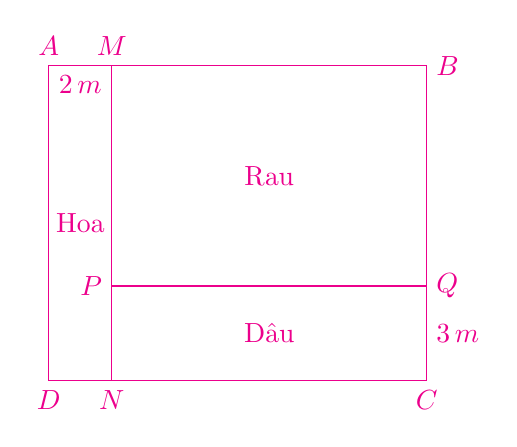
\begin{tikzpicture}[scale=0.4,toancuabi]
			\draw (0,0) rectangle (12,10);
			\draw (2,0) -- (2,10) (2,3) -- (12,3);
			\draw (0,0) node[below] {$D$};
			\draw (2,0) node[below] {$N$};
			\draw (12,0) node[below] {$C$};
			\draw (2,3) node[left] {$P$};
			\draw (12,3) node[right] {$Q$};
			\draw (12,10) node[right] {$B$};
			\draw (2,10) node[above] {$M$};
			\draw (0,10) node[above] {$A$};
			\draw (1,10) node[below] {$2\,m$};
			\draw (1,5) node {Hoa};
			\draw (7,1.5) node {Dâu};
			\draw (7,6.5) node {Rau};
			\draw (12,1.5) node[right] {$3\,m$};
		\end{tikzpicture}
		\vspace*{-10pt}
	\end{figure}
	Phần trồng hoa là hình chữ nhật $AMND$ có diện tích là $20\,m^2$. Hình chữ nhật AMND có cạnh $AM=2\,m$ nên cạnh còn lại $AD=10\,m$.
	\vskip 0.1cm
	Khu vườn là hình chữ nhật $ABCD$ có diện tích $120\, m^2$. Hình chữ nhật $ABCD$ có cạnh $AD=10\,m$ nên cạnh $DC = 12\,m$.
	\vskip 0.1cm
	Ta có
	$DC = 12 = DN + NC = 2 + NC$. Do đó $NC=10$.
	\vskip 0.1cm
	Từ đó, phần trồng dâu là hình chữ nhật $PQCN$ có hai cạnh $NC=10$ và $QC=3$. Do đó diện tích của phần trồng dâu là: $30\,m^2$.
	\vskip 0.1cm
	Vậy diện tích của phần trồng rau là: $120 - 20 - 30 = 70\,m^2$. 
	\vskip 0.1cm
	\textbf{\color{toancuabi}Bài $\pmb6$.}
	Mỗi bạn được chia $30: 3=10$ chiếc kẹo.
	\vskip 0.1cm
	Do Bình ăn một số kẹo bằng với số kẹo mà An còn nên tổng số kẹo mà An và Bình ăn là $10$ chiếc. Vì thế tổng số kẹo mà An, Bình và Chi ăn là $10+10=20$ chiếc. Do vậy, còn lại $30-20=10$ chiếc kẹo.
	\vskip 0.1cm
	\textbf{\color{toancuabi}Bài $\pmb7$.} Gọi số cây quất là $n$. Khi đó tổng tiền bán được của lần bán đầu khi cây cuối có giá $230$ nghìn là $245\times n$ và tổng tiền thu được khi bán cây cuối với giá $158$ nghìn là $242\times n$. Ta thấy chênh lệch giữa giá bán cây cuối ở $2$ lần bằng $3\times n$. Do số tiền chênh lệch giữa hai lần bán là: 
	\begin{align*}
		230-158=72 \text{ nghìn}
	\end{align*}
	nên bác nông dân đã bán được 
	\begin{align*}
		72:3 = 24 \text{ cây quất.}
	\end{align*}
	\textbf{\color{toancuabi}Bài $\pmb8$.} Ta thấy
	Cột $1$ có $2$ cách xếp bi;
	\vskip 0.1cm
	Cột $3$ có $2$ cách xếp bi;
	\vskip 0.1cm
	Cột $5$ có $1$ cách xếp  bi;
	\vskip 0.1cm
	Cột $2$ có $1$ cách xếp  bi;
	\vskip 0.1cm
	Cột $4$ có $1$ cách xếp  bi.
	\vskip 0.1cm
	Do đó, số cách xếp bi là: $2\times 2\times 1\times 1\times 1 = 4$ (cách)
	\vskip 0.1cm
	\textbf{\color{toancuabi}Bài $\pmb9$.} Gọi hai số còn khuyết ở hàng cuối là $a$ và $b$. Do mỗi ô ở hàng trên bằng tổng hai ô ngay bên dưới nên ta điền được các số như sau.
	\begin{figure}[H]
		\vspace*{-5pt}
		\centering
		\captionsetup{labelformat= empty, justification=centering}
		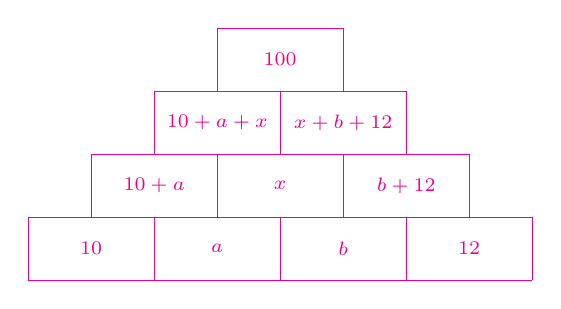
\begin{tikzpicture}[xscale=2, toancuabi,scale=0.8, node font=\scriptsize]
			\draw (0,0) grid (4,1);
			\draw (1,2) grid (3,3);
			\draw (0.5,1) rectangle (3.5,2);
			\draw (1.5,3) rectangle (2.5,4);
			\draw (1.5,1) --(1.5,2) (2.5,1) --(2.5,2);
			\draw (0.5,0.5) node {$10$};
			\draw (1.5,0.5) node {$a$};
			\draw (2.5,0.5) node {$b$};
			\draw (3.5,0.5) node {$12$};
			\draw (1,1.5) node {$10 + a $};
			\draw (2,1.5) node {$x$};
			\draw (3,1.5) node {$b+ 12$};
			\draw (1.5,2.5) node {$10 + a + x$};
			\draw (2.5,2.5) node {$x + b + 12$};
			\draw (2,3.5) node {$100$};
		\end{tikzpicture}
		\vspace*{-10pt}
	\end{figure}
	Vậy $100 = a + 10 + x + b + 12 + x = a + b + 2×x + 22$.
	\vskip 0.1cm
	Do $x = a + b$ nên $100 = 3\times x + 22$.
	\vskip 0.1cm
	Giải ra ta được $x = 26$.
	\vskip 0.1cm
	\textbf{\color{toancuabi}Bài $\pmb{10}$.} Mã PIN của bạn Kiên có dạng: $1ab3$, với $a$, $b$ là hai chữ số khác nhau và khác hai chữ số $1$, $3$.
	\vskip 0.1cm
	Ta thấy có $8$ cách chọn chữ số $a$ và $7$ cách chọn chữ số $b$.
	\vskip 0.1cm
	Do đó có $8\times 7 = 56$ cách chọn $2$ chữ số $a$ và $b$ hay có $56$ số khác nhau cho mã PIN của bạn Kiên.
\end{multicols}
%\newpage
%\graphicspath{{../toancuabi/pic/}}
%\begingroup
%\AddToShipoutPicture*{\put(106,650){
\includegraphics[scale=1]{../tieude.pdf}}}  
%\centering
%\endgroup
%\vspace*{55pt} 
%\begin{multicols}{2}
%	Thám tử Xuân Phong đôi khi phải đột nhập vào những nơi hoang vắng, kỳ bí để tìm ra được dấu tích của những kẻ gây án. Một lần nọ, sau bao ngày cải trang để bám sát, theo dõi manh mối, thám tử biết tên trùm tội phạm đang trốn tránh trong một ngôi nhà hẻo lánh ở ngoại ô. Vừa đến trước cửa của ngôi nhà gỗ cổ kính, Xuân Phong gặp một bà lão với đôi mắt tinh anh nhìn mình với vẻ bí mật ``thám tử đó phải không, tôi nhận ngay ra ngài, dù ngài đã cải trang rất kỹ. Phải chăng thám tử đang đi tìm tên trùm? Hắn đang ngồi dưới kia, trong căn phòng cùng những người trong Hiệp hội Thương Gia, nhưng vô cùng nguy hiểm nếu ngài dùng vũ lực ở đây để bắt hắn. Tôi mách ngài nhé, ở dưới đó, có $10$ người, trong đó có lão trùm và những kẻ đồng phạm của lão. Bọn họ là những kẻ luôn nói dối, nhưng cũng có thể có cả những người lương thiện, luôn nói thật, ở ngay bên cạnh. Ngài hãy dùng trí thông minh của mình, chỉ được hỏi rất hạn chế câu hỏi để phán đoán ra những kẻ phạm tội là ai. Ngài hỏi nhiều câu hơn sẽ nguy hiểm cho cả những thương gia lương thiện có thể có mặt ở đó. Và ngài hãy hứa với bà lão này sẽ đảm bảo an toàn cho tôi và gia đình, vì tôi đã liều mình thông báo tin mật này với thám tử".
%	\vskip 0.1cm
%	Theo lời bà lão mách bảo, Xuân Phong lần theo một chiếc cầu thang cũ nát và đi xuống một căn phòng khuất dưới tầng hầm. Vừa mở cửa ra, thám tử đã thấy có $10$ người ăn mặc chỉnh tề như nhau, ngồi nghiêm trang quanh một chiếc bàn mười cạnh, mỗi người ngồi tại đỉnh của hình mười cạnh. Ánh sáng lờ mờ trong phòng đủ chiếu rõ dòng chữ ``Cuộc họp thường niên Hiệp hội Thương gia -- Khu vực Duyên Hải". Thật khó để xác định ai là kẻ nói dối trong số họ, vì vẻ ngoài họ đều giống như những thương Gia thường gặp: quyền lực, sắc sảo và oai vệ.
%	\begin{figure}[H]
%		\centering
%		\vspace*{-5pt}
%		\captionsetup{labelformat= empty, justification=centering}
%		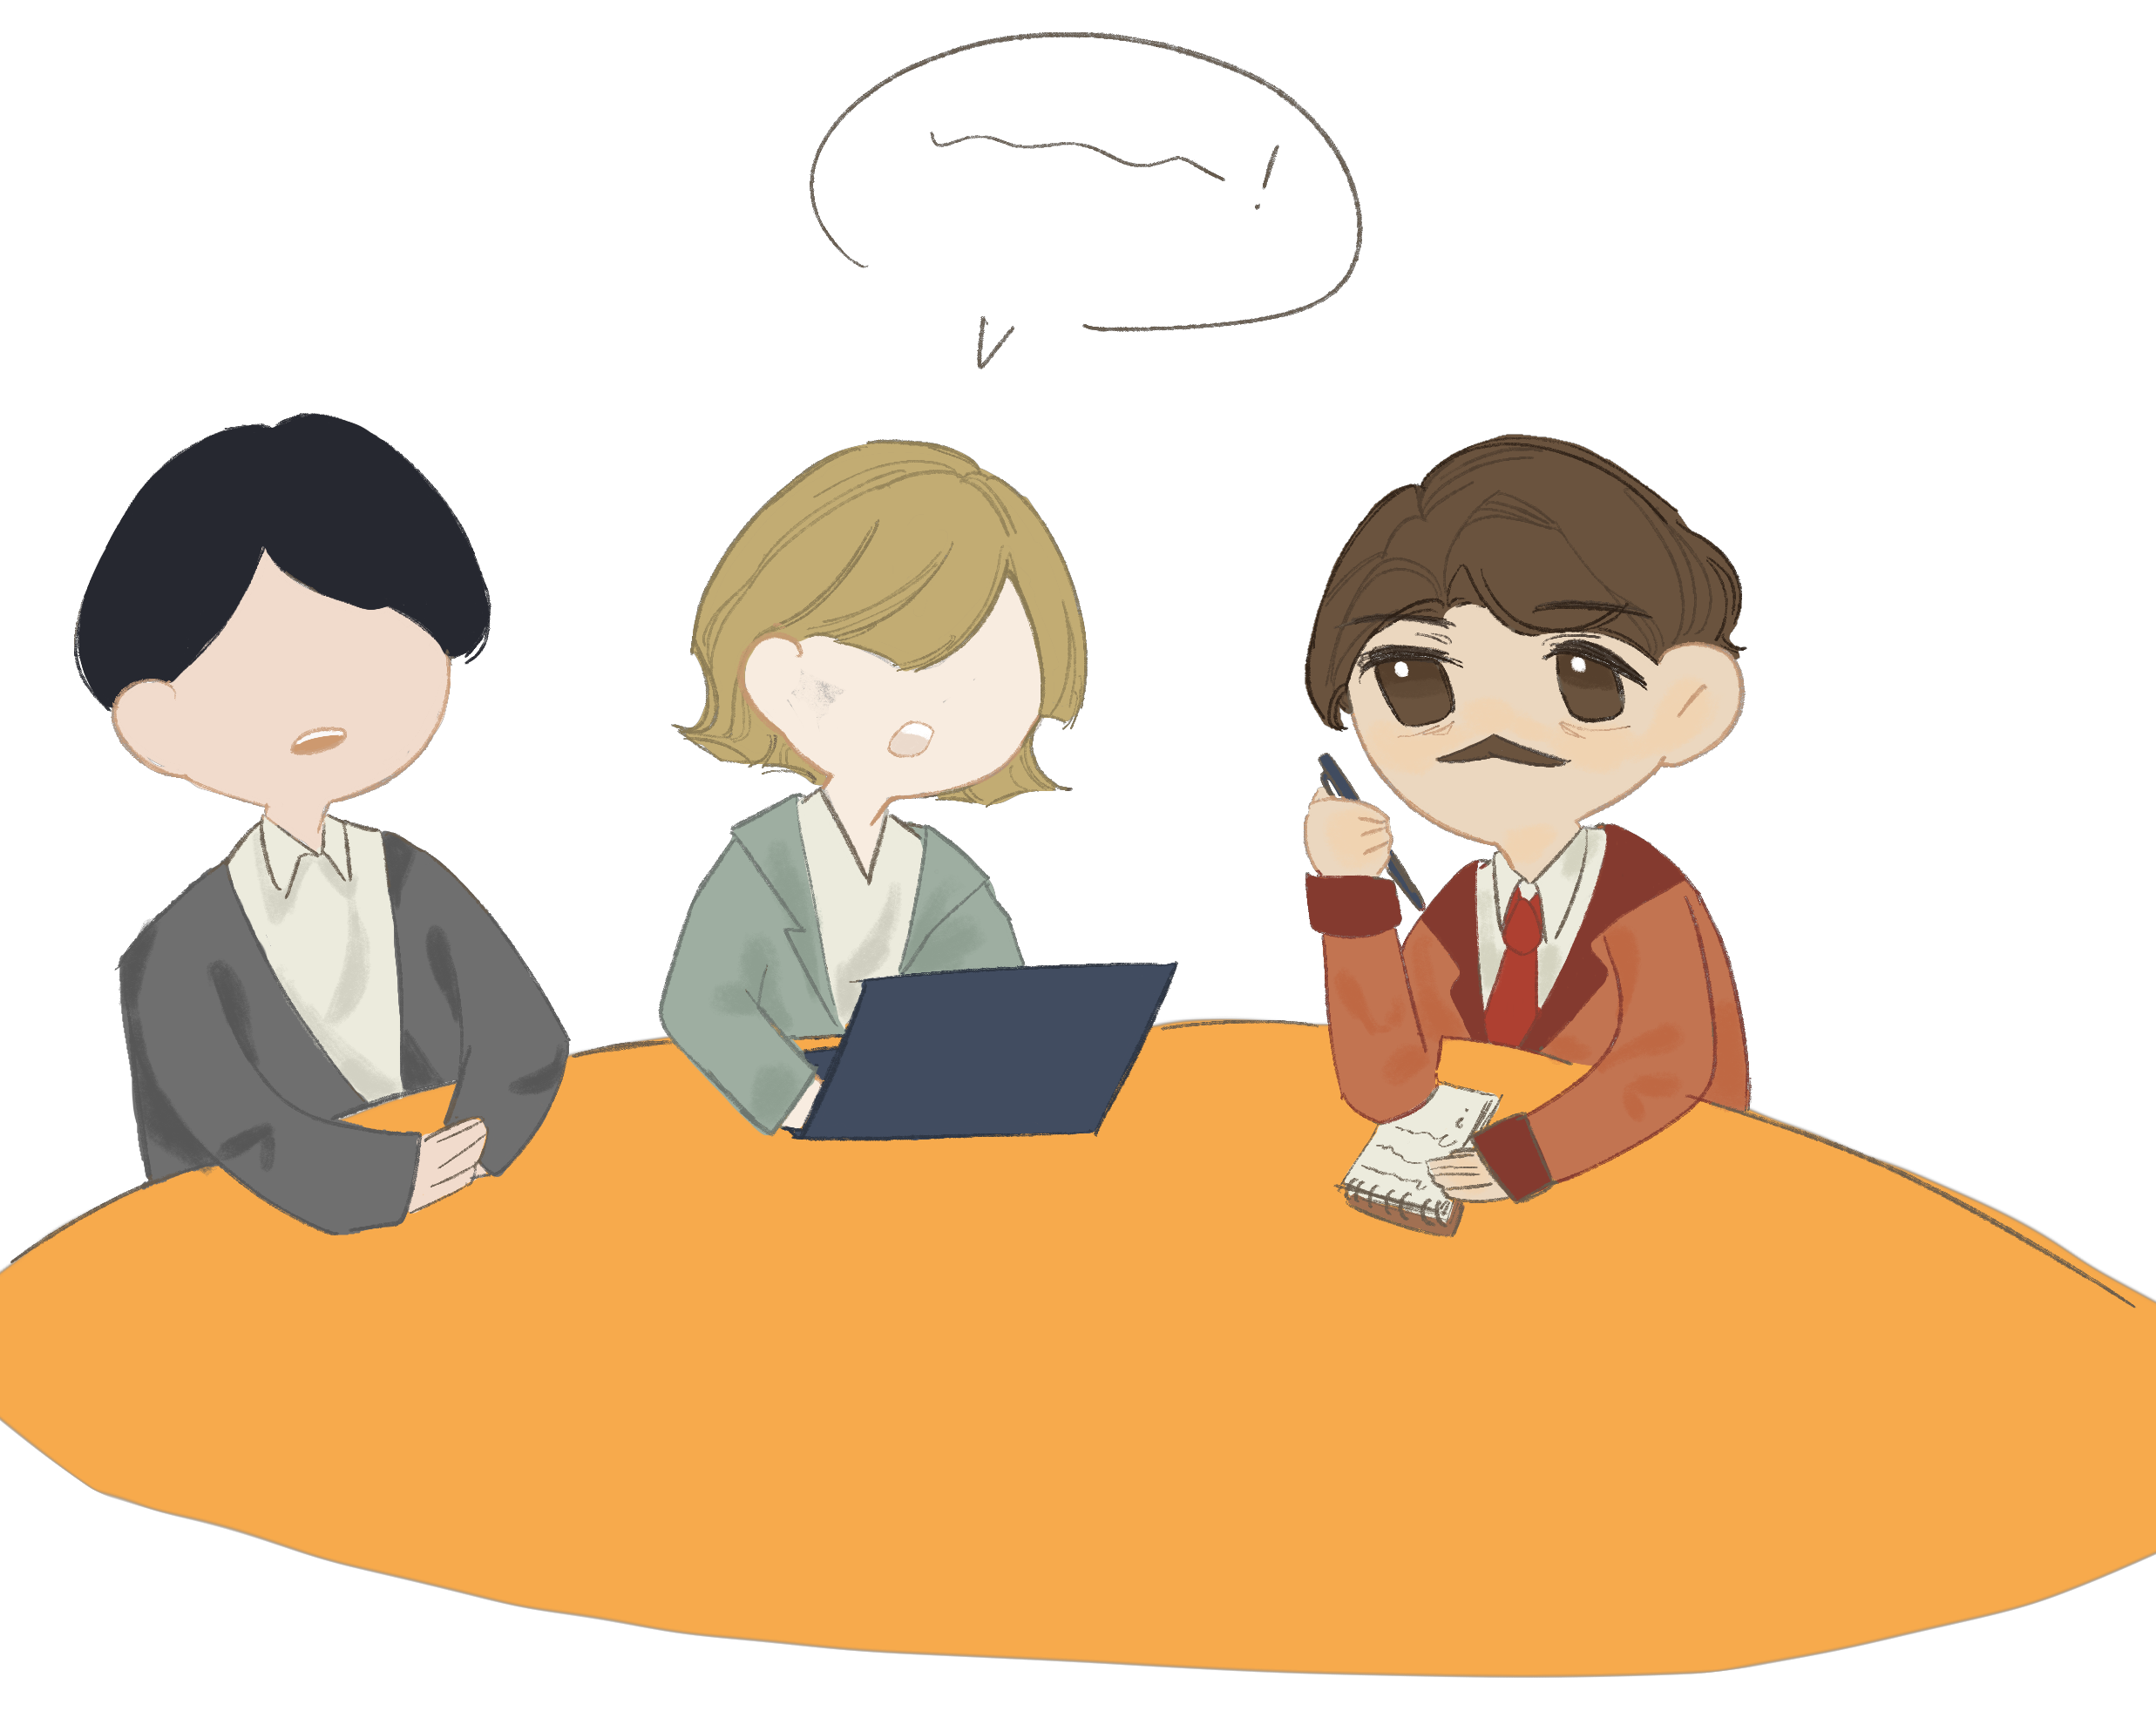
\includegraphics[width=1\linewidth]{xp}
%		\vspace*{-15pt}
%	\end{figure}
%	Theo quy định của Hiệp hội Thương gia dành cho những người ngoài, qua lời của bà lão, thám tử có thể đứng dậy bước tới một nơi bất kỳ nào đó trong căn phòng và chỉ được hỏi câu hỏi ``Khoảng cách từ chỗ tôi đứng đến người nói dối gần nhất trong số các anh là bao nhiêu?" cho tất cả những người trong phòng. Sau đó, mỗi người trong số $10$ người ngồi xung quanh bàn sẽ trả lời thám tử, lúc này đã cải trang thành một thương gia muốn gia nhập Hiệp hội. thám tử không được phép đứng lên mặt bàn và tất cả mọi người, kể cả thám tử, đều được phép dùng thước để đo khoảng cách tuỳ ý. Ta cũng được biết rằng ngoài $10$ người và thám tử, trong phòng không còn có người lạ nào khác, hơn nữa $10$ người đều biết rõ ai trong số họ là nói thật và ai trong số họ là nói dối. Em hãy cho biết Xuân Phong có thể sử dụng ít nhất bao nhiêu câu hỏi như trên để biết chắc chắn ai trong số những người ngồi quanh bàn là nói~dối?
%\end{multicols}
%\newpage
%\begingroup
%\AddToShipoutPicture*{\put(115,670){
\includegraphics[scale=1]{../tieude11.pdf}}} 
%\centering
%\endgroup
%\vspace*{35pt}
%
%\begin{multicols}{2}
%	$\pmb{1.}$ Tuấn và Tú cùng tham gia một giải thi đấu cờ vua cùng các bạn học sinh khác trong trường. Hai bạn tổng cộng ghi được $6{.}5$ điểm, trong khi tất cả các bạn học sinh còn lại đều ghi được số điểm bằng nhau. Hỏi có tất cả bao nhiêu học sinh tham gia giải cờ vua đó? (Biết rằng trong giải thi đấu, mỗi người tham gia thi đấu đúng một ván với mỗi người còn lại, ghi được $1$ điểm sau mỗi trận thắng, $0{.}5$ điểm sau mỗi trận hoà và $0$ điểm sau mỗi trận thua).
%	\begin{figure}[H]
%		\centering
%		\vspace*{-5pt}
%		\captionsetup{labelformat= empty, justification=centering}
%		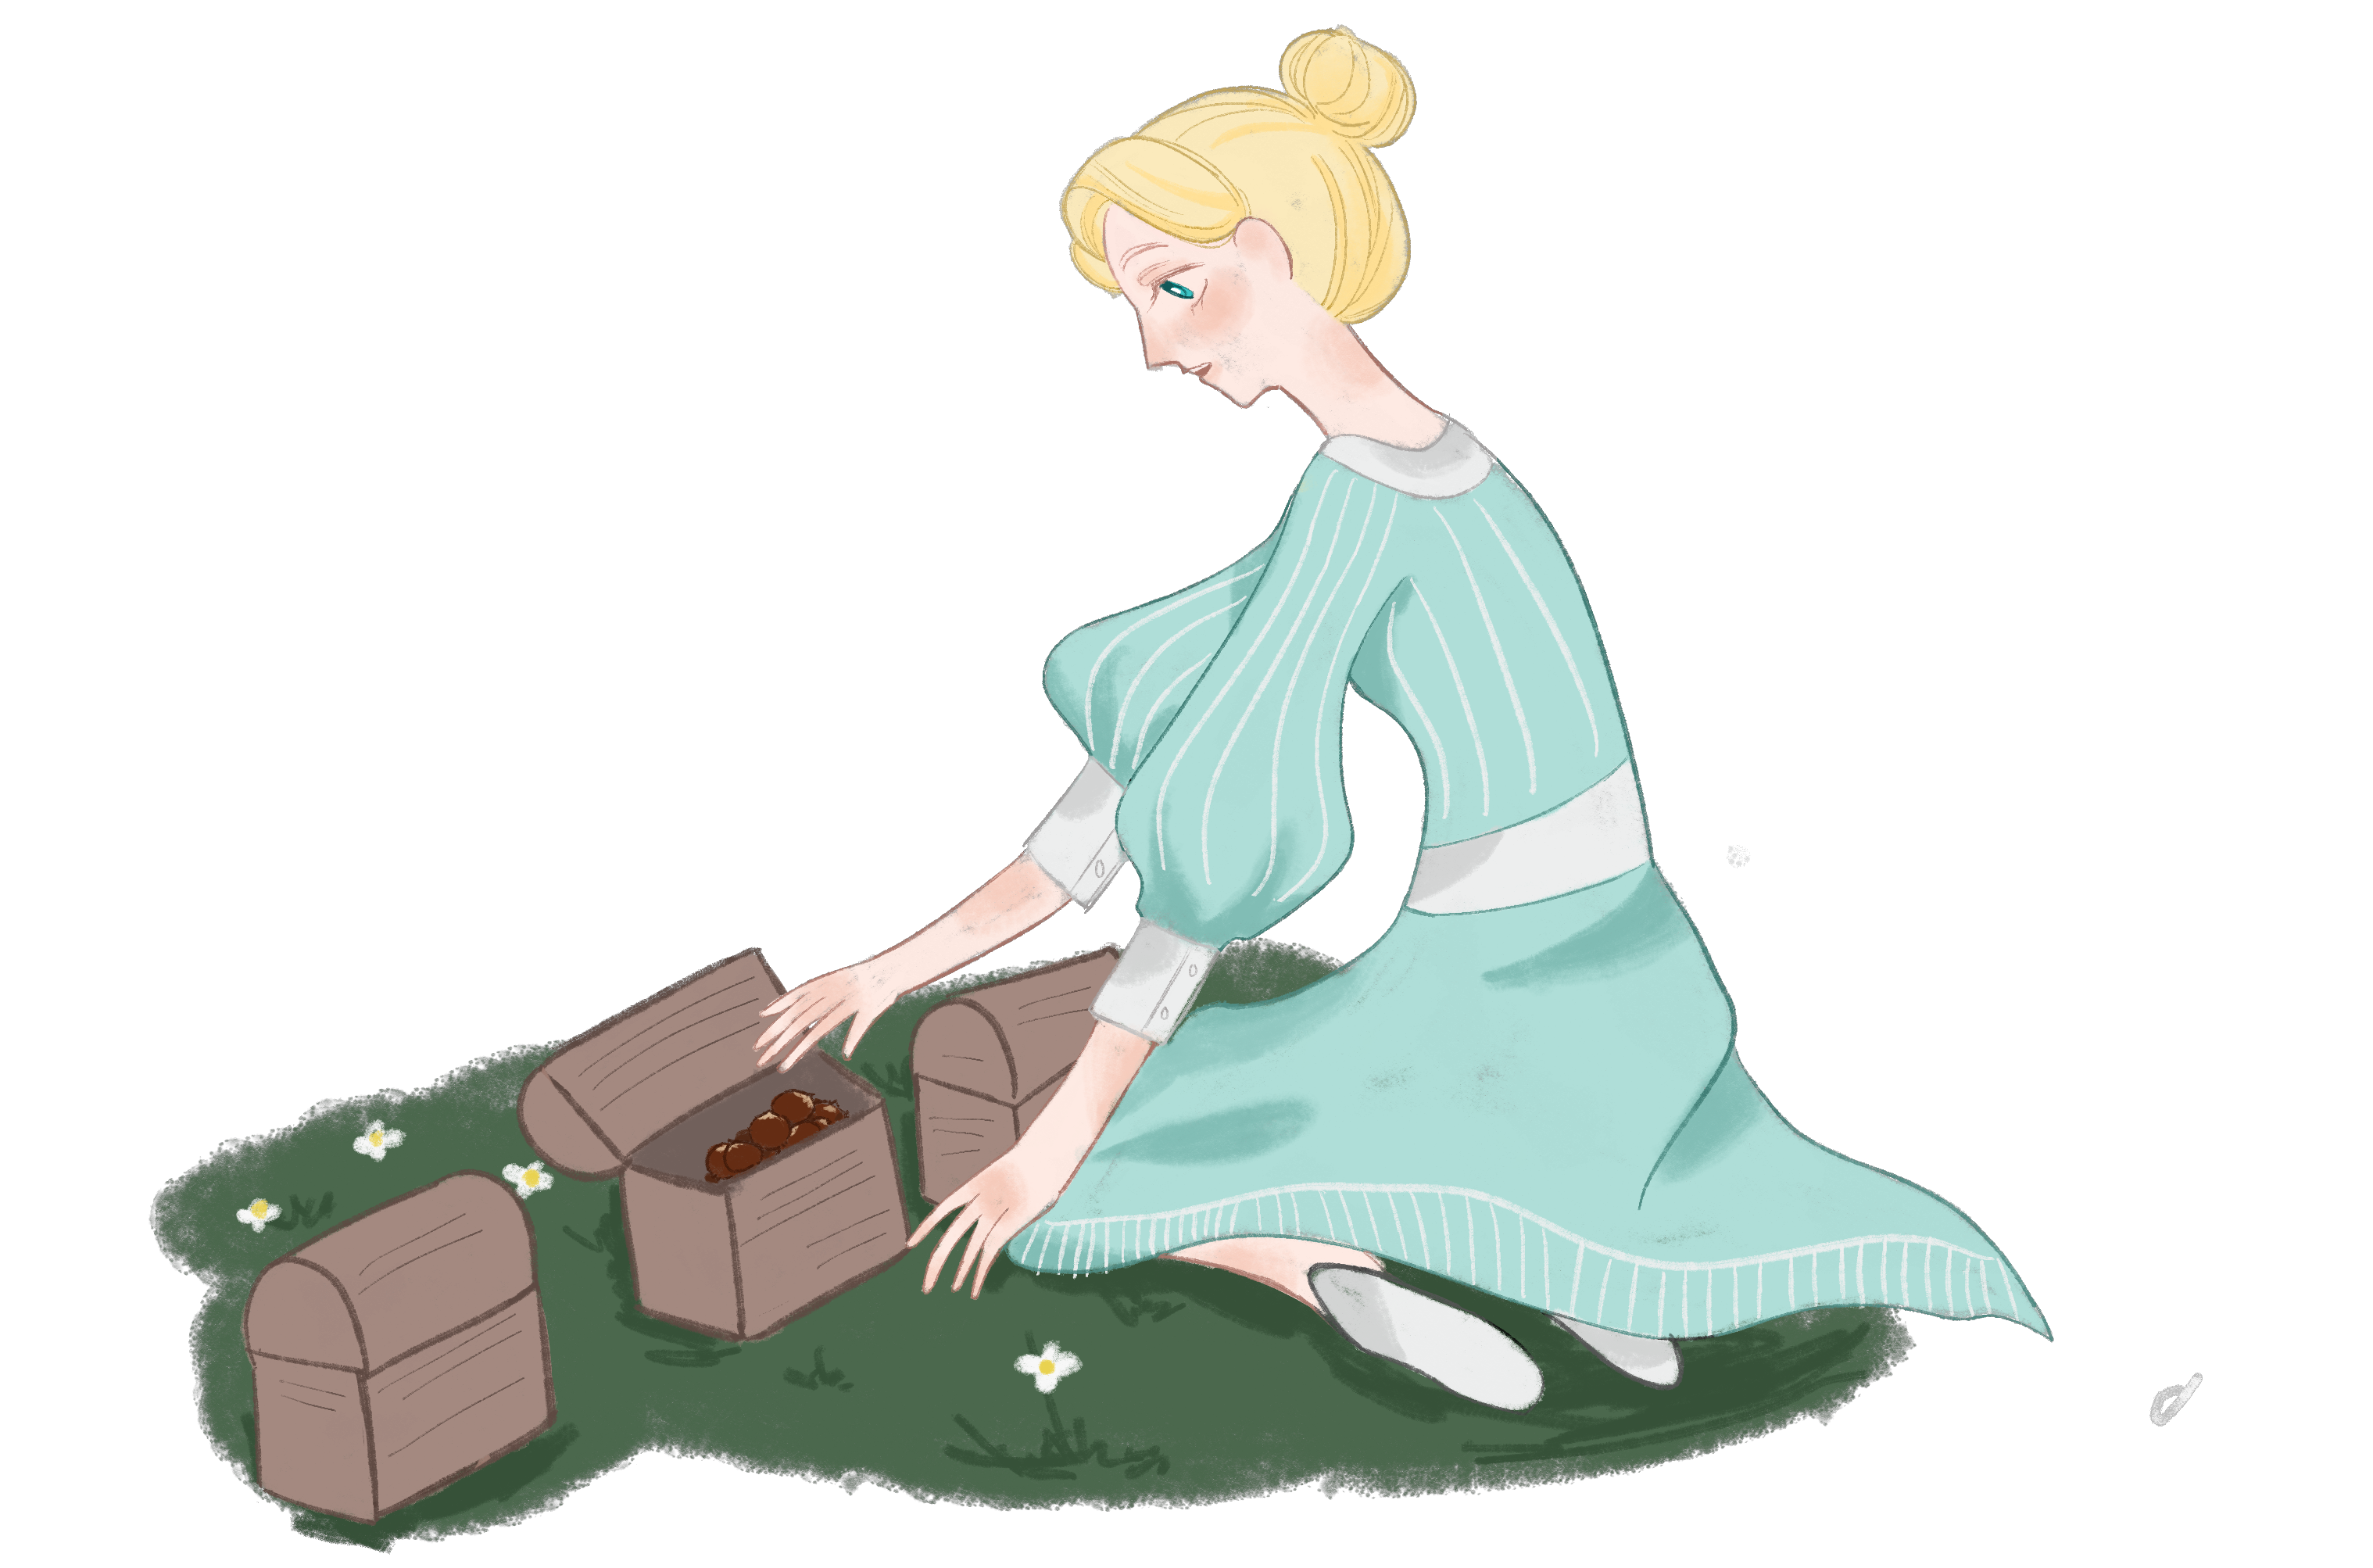
\includegraphics[width=1\linewidth]{Hinh1}
%		\vspace*{-20pt}
%	\end{figure}
%	$\pmb{2.}$ 	Lớp $6$A gồm $22$ bạn chia thành hai đội: Xanh gồm các bạn nam và Đỏ gồm các bạn nữ để tổ chức thi tài đối đáp, trả lời thông minh. Đầu tiên, bạn Hoa ở nhóm Đỏ đối đáp với $6$ bạn nam ở nhóm Xanh và giành chiến thắng. Tiếp theo, bạn Mai ở nhóm Đỏ đối đáp với $7$ bạn nam ở nhóm Xanh và cũng giành chiến thắng. Tiếp tục bạn Huệ ở nhóm Đỏ cũng chiến thắng $8$ bạn nam ở nhóm Xanh. Cứ tiếp tục như vậy, cuối cùng bạn Hà ở nhóm Đỏ đã đối đáp thông minh với toàn bộ các bạn nam ở nhóm Xanh và giành chiến thắng chung cuộc. Hỏi trong lớp có tất cả bao nhiêu bạn nam?
%	\begin{figure}[H]
%		\centering
%		\vspace*{-5pt}
%		\captionsetup{labelformat= empty, justification=centering}
%		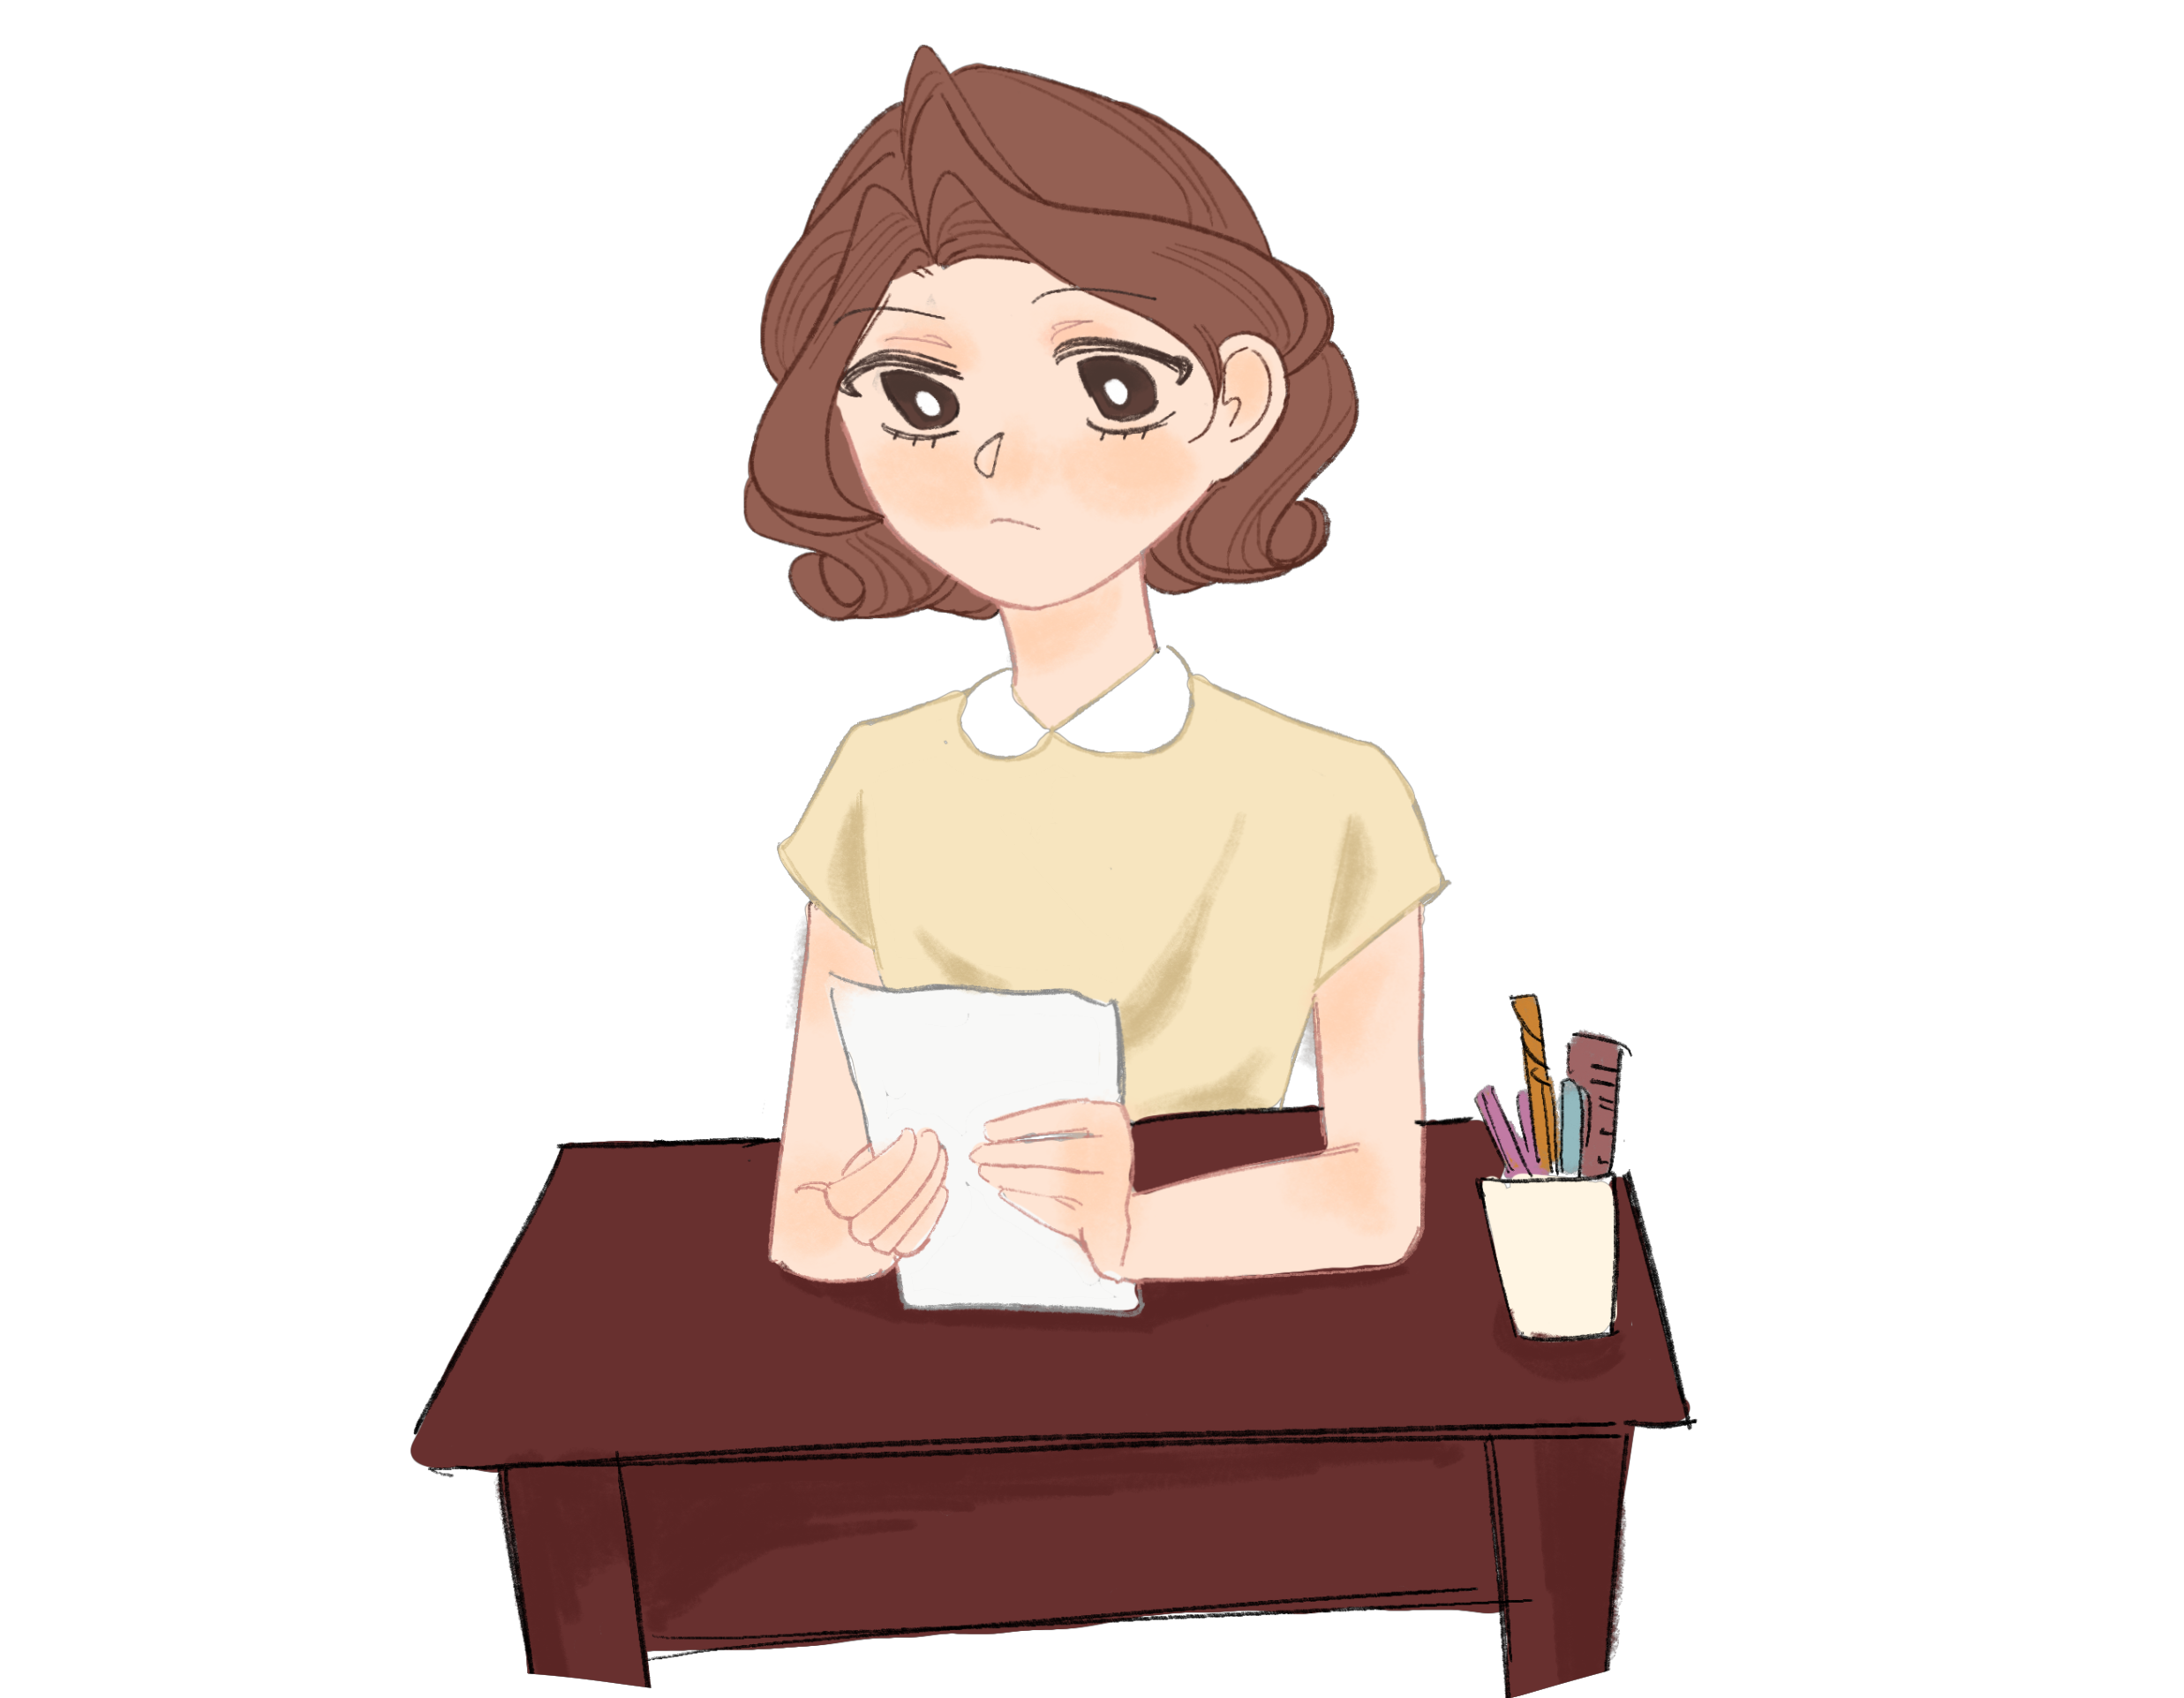
\includegraphics[width=1.01\linewidth]{Hinh2}
%		\vspace*{-5pt}
%	\end{figure}
%	$\pmb{3.}$ 	Có bốn chủ doanh nghiệp tới thăm trường học cũ của mình, mang theo một số món quà với dự định sẽ trao tặng cho các học sinh đang học ở đó. Khi tất cả $252$ em học sinh được mời xếp thành một hàng ngang, chủ doanh nghiệp thứ nhất tặng quà cho mỗi em đứng thứ tư trong hàng (các em ở số thứ tự $4,8,12,$ \ldots). Chủ doanh nghiệp thứ hai lại tặng quà cho mỗi em đứng thứ bảy (các em ở số thứ tự $7,14,21$, \ldots). Chủ doanh nghiệp thứ ba trao tặng quà cho mỗi em đứng thứ mười một (các em ở số thứ tự $11,22,33$, \ldots). Chủ doanh nghiệp thứ tư sẽ tặng quà cho các em còn lại. Hỏi có bao nhiêu em học sinh nhận được quà từ mỗi chủ doanh nghiệp?
%	\begin{figure}[H]
%		\centering
%		\vspace*{-5pt}
%		\captionsetup{labelformat= empty, justification=centering}
%		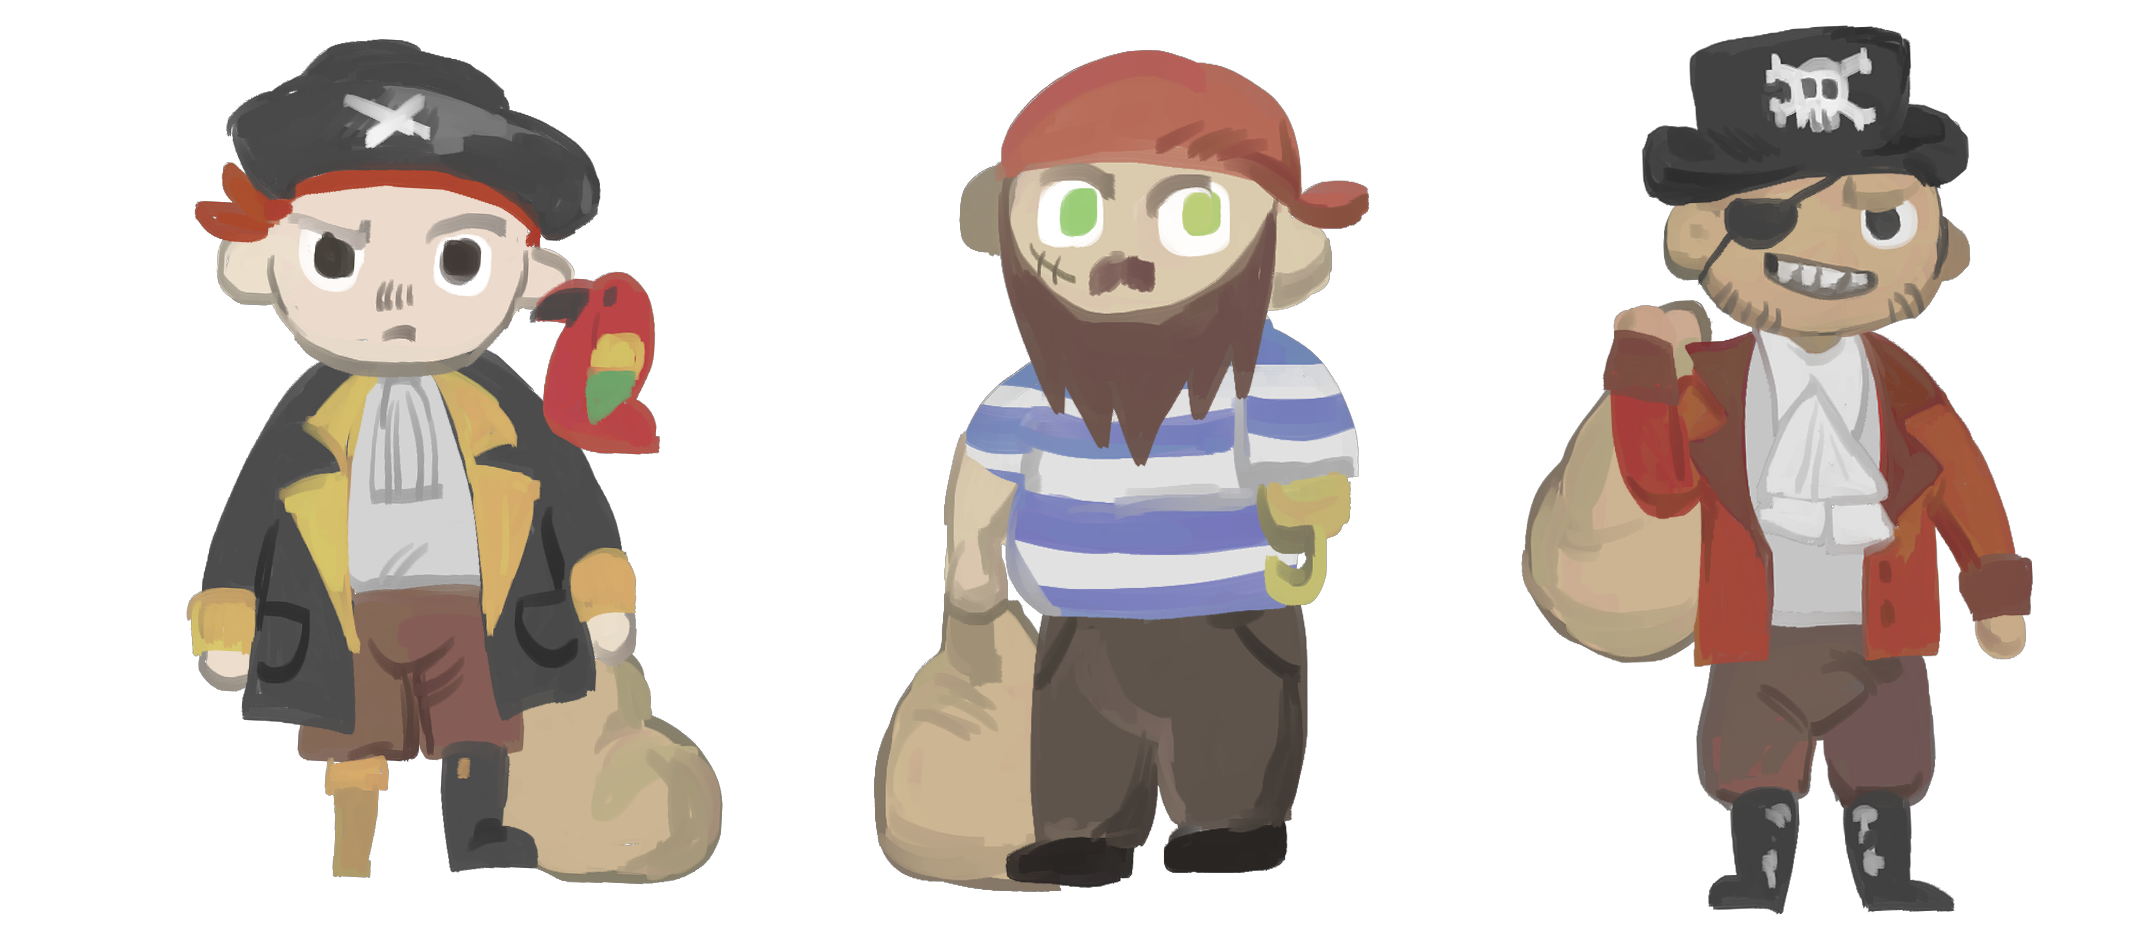
\includegraphics[width=1\linewidth]{Hinh3}
%		\vspace*{-15pt}
%	\end{figure}
%	$\pmb{4.}$ 	Có ba nhà tài trợ quyết định giúp đỡ một tạp chí khoa học thường thức với tên gọi là Phi. Nhà tài trợ Quốc trao tặng một khoản tiền tính bằng dollar gồm có $4$ chữ số: $2$ chữ số đứng trước dấu phẩy, và hai chữ số sau dấu phẩy, trong đó số cent lẻ (tức là hai chữ số đứng sau dấu phẩy) bằng với đúng số dollar chẵn (tức là hai chữ số đứng trước dấu phẩy; ta nhớ lại $100$ cent $= 1$ dollar). Nhà tài trợ Minh tặng số tiền với số dollar chẵn lớn hơn $3$ dollar so với số dollar chẵn mà nhà tài trợ Quốc đã tặng nhưng số cent lẻ lại ít hơn $8$ lần số cent lẻ của nhà tài trợ Quốc. Nhà tài trợ Vũ hào phóng đem tặng số tiền bằng $1/7$ tổng số tiền của hai nhà tài trợ Quốc và Minh đã trao cộng lại. Hỏi số tiền ủng hộ của ba nhà tài trợ cho tạp chí Phi là bao nhiêu?
%	\begin{figure}[H]
%		\centering
%%		\vspace*{-5pt}
%		\captionsetup{labelformat= empty, justification=centering}
%		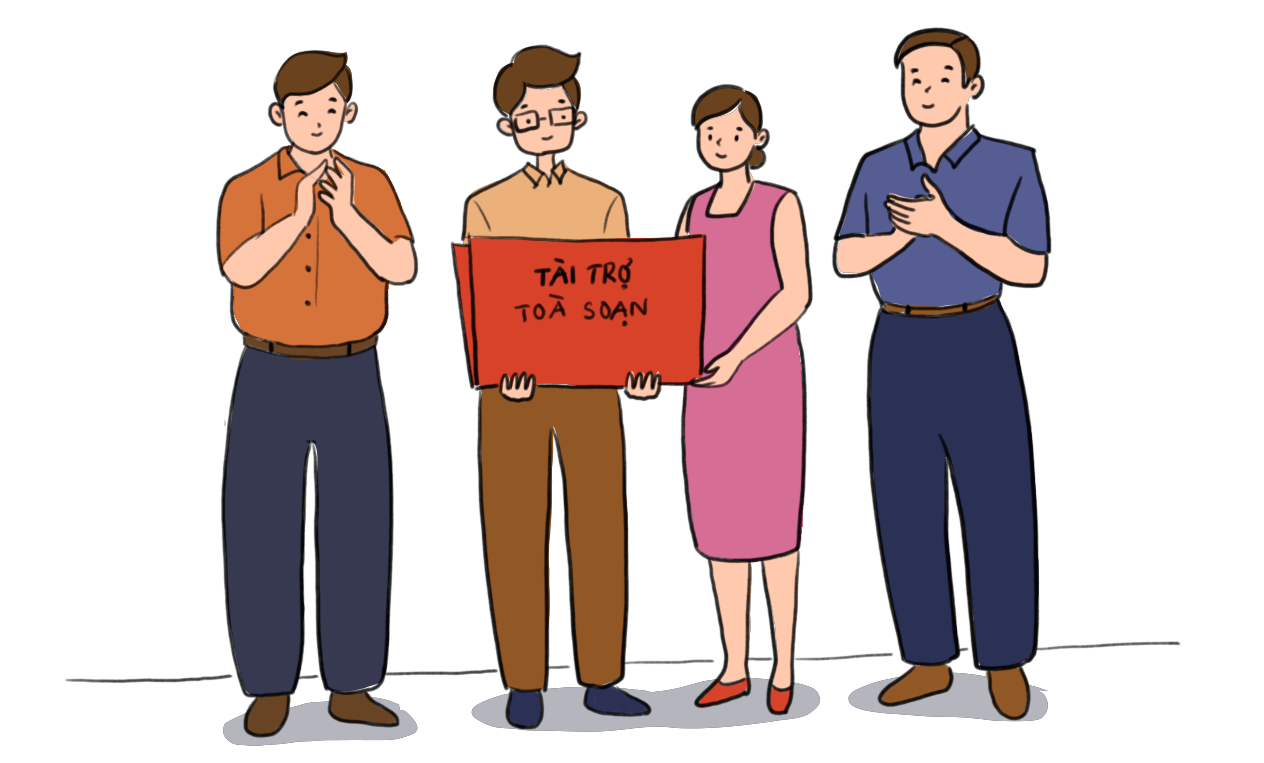
\includegraphics[width=0.8\linewidth]{Hinh4}
%		\vspace*{-10pt}
%	\end{figure}
%	\vskip 0.1cm
%	$\pmb{5.}$ 	Trên hòn đảo Ngọc ở giữa một đại dương xanh ngắt có $100$ thổ dân sinh sống, một số người trong họ luôn nói dối, còn những người còn lại luôn nói thật. Mỗi một thổ dân thờ phụng đúng một trong ba vị thần: thần Mặt trời, thần Mặt trăng hoặc thần Đất. Người ta hỏi mỗi thổ dân ba câu hỏi sau đây:
%	\begin{figure}[H]
%		\centering
%		\vspace*{-5pt}
%		\captionsetup{labelformat= empty, justification=centering}
%		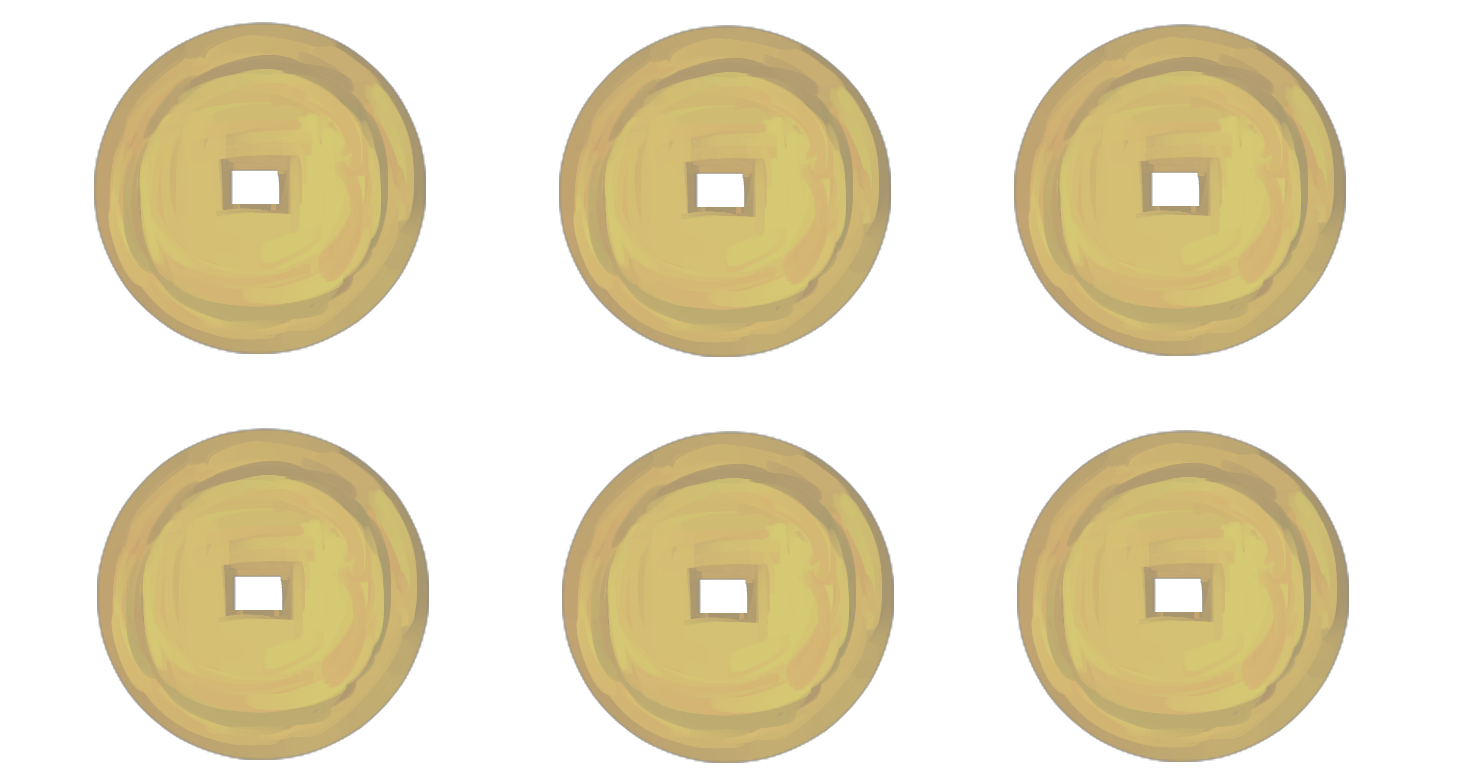
\includegraphics[width=1\linewidth]{Hinh5}
%		\vspace*{-20pt}
%	\end{figure}
%	$1.$ Ông (bà) có thờ phụng thần Mặt trời hay không?
%	\vskip 0.1cm
%	$2.$ Ông (bà) có thờ phụng thần Mặt trăng hay không?
%	\vskip 0.1cm
%	$3.$ Ông (bà) có thờ phụng thần Đất hay không?
%	\vskip 0.1cm
%	Có $60$ người trả lời khẳng định ``có" với câu hỏi thứ nhất, $40$ người trả lời khẳng định ``có" với câu hỏi thứ hai và $30$ người trả lời khẳng định ``có" với câu hỏi thứ ba. Hỏi trên đảo Ngọc có bao nhiêu thổ dân nói dối?
%	\vskip 0.1cm
%	$\pmb{6.}$ 	Có $100$ em học sinh được mời tới buổi tổng kết cuối năm học của nhà trường. Các ghế trong phòng họp được xếp ngay ngắn thẳng hàng theo dạng một hình vuông với $10$ dãy ghế, mỗi dãy có đúng $10$ chiếc ghế. Buổi họp phải diễn ra muộn hơn do bị cắt điện, vì thế các em học sinh bắt đầu bàn luận trao đổi với các bạn bên cạnh về kết quả điểm trung bình của mình. Em học sinh nào thấy trong tất cả những bạn ngồi kề sát mình: bên trái, bên phải, đằng sau, đằng trước và theo các đường chéo, chỉ có tối đa một bạn có điểm trung bình cao hơn hoặc bằng điểm trung bình của  mình, sẽ tự coi mình là ``có thành tích".
%	\begin{figure}[H]
%		\centering
%		\vspace*{-10pt}
%		\captionsetup{labelformat= empty, justification=centering}
%		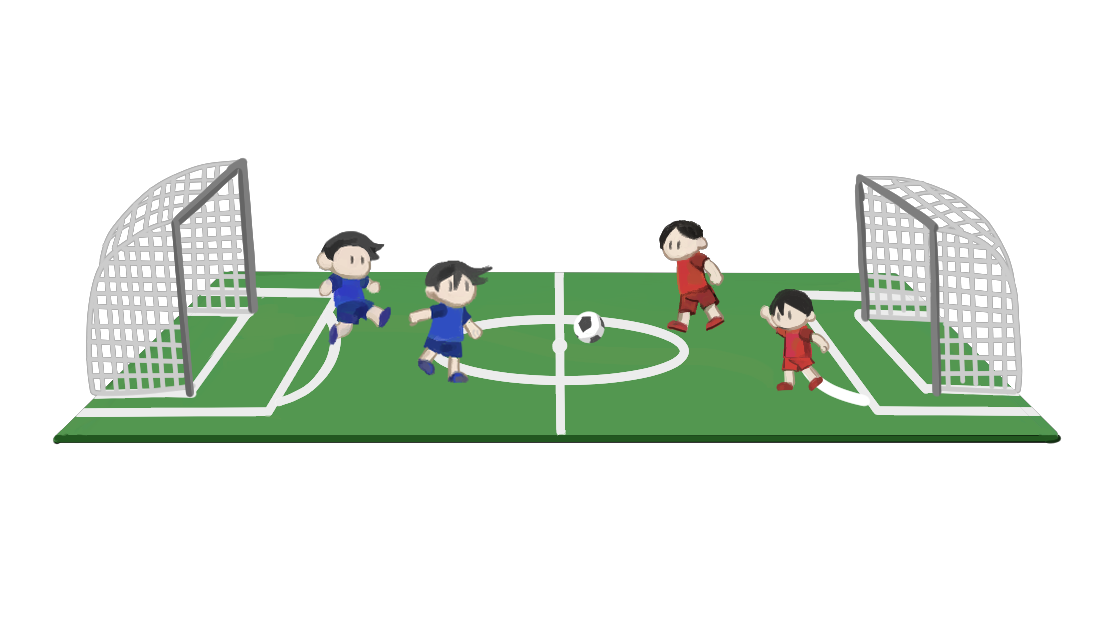
\includegraphics[width=0.85\linewidth]{Hinh6}
%		\vspace*{-10pt}
%	\end{figure}
%	Hỏi trong buổi họp đó có thể có tối đa bao nhiêu em học sinh đã tự coi mình là ``có thành tích" trong học tập?
%\end{multicols}
%\vspace*{-10pt}
%{\color{toancuabi}\rule{1\linewidth}{0.1pt}}
%\begingroup
%\AddToShipoutPicture*{\put(114,178){
\includegraphics[scale=1]{../tieude2.pdf}}} 
%\centering
%\endgroup
%\vspace*{75pt}
%
%\begin{multicols}{2}
%	$\pmb{1.}$ Các bạn nam mang kẹo tới lớp để tặng cho các bạn nữ. Bạn Phúc nói rằng mình đã mang tới đúng một nửa tổng số kẹo. Bạn Kiên nói rằng mình đã mang tới đúng một phần ba tổng số kẹo và chỉ chia kẹo của mình cho Mai và Tuyết, hơn nữa Mai được nhiều hơn so với Tuyết là $3$ chiếc kẹo. Em hãy chứng tỏ rằng có một bạn trong số Phúc và Kiên đã \linebreak nhầm lẫn.\\
%	\textit{Lời giải.} Giả sử cả hai bạn Phúc và Kiên đều không nhầm lẫn. Do Phúc không nhầm, nên tổng số kẹo được mang tới lớp phải là số chẵn (gấp $2$ lần số kẹo mà Phúc mang tới). Do Kiên cũng mang tới một số kẹo là số nguyên, bằng $1/3$ của một số chẵn, nên Kiên cũng mang tới một số kẹo là số chẵn. Theo lời của Kiên, số kẹo mà cậu đã tặng cho các bạn nữ là một số lẻ, do số kẹo mà Mai và Tuyết nhận được khác tính chẵn lẻ (hơn kém nhau là $3$ chiếc, mà $3$ là một số lẻ), mà tổng của hai số khác tính chẵn lẻ là một số lẻ. Ta nhận được mâu thuẫn. Suy ra có ít nhất một bạn nam trong số Phúc và Kiên đã nhầm lẫn.
%	\begin{figure}[H]
%			\centering
%		\vspace*{-5pt}
%		\captionsetup{labelformat= empty, justification=centering}
%		
\includegraphics[width=0.6\linewidth]{Pi7_bai1}
%		\vspace*{-10pt}
%	\end{figure}
%	$\pmb{2.}$ Ba người thợ cùng đào một chiếc hố. Họ luân phiên lần lượt làm việc, mỗi người làm việc trong một thời gian nhất định. Nếu trong khi một người làm việc hai người còn lại cũng đồng thời đào hố thì hai người này sẽ đào được đúng một nửa hố. Hỏi nếu cả ba người cùng đồng thời đào thì họ sẽ làm nhanh hơn được bao nhiêu lần so với cách làm luân phiên ban đầu?
%	\begin{figure}[H]
%		\centering
%		\vspace*{-5pt}
%		\captionsetup{labelformat= empty, justification=centering}
%		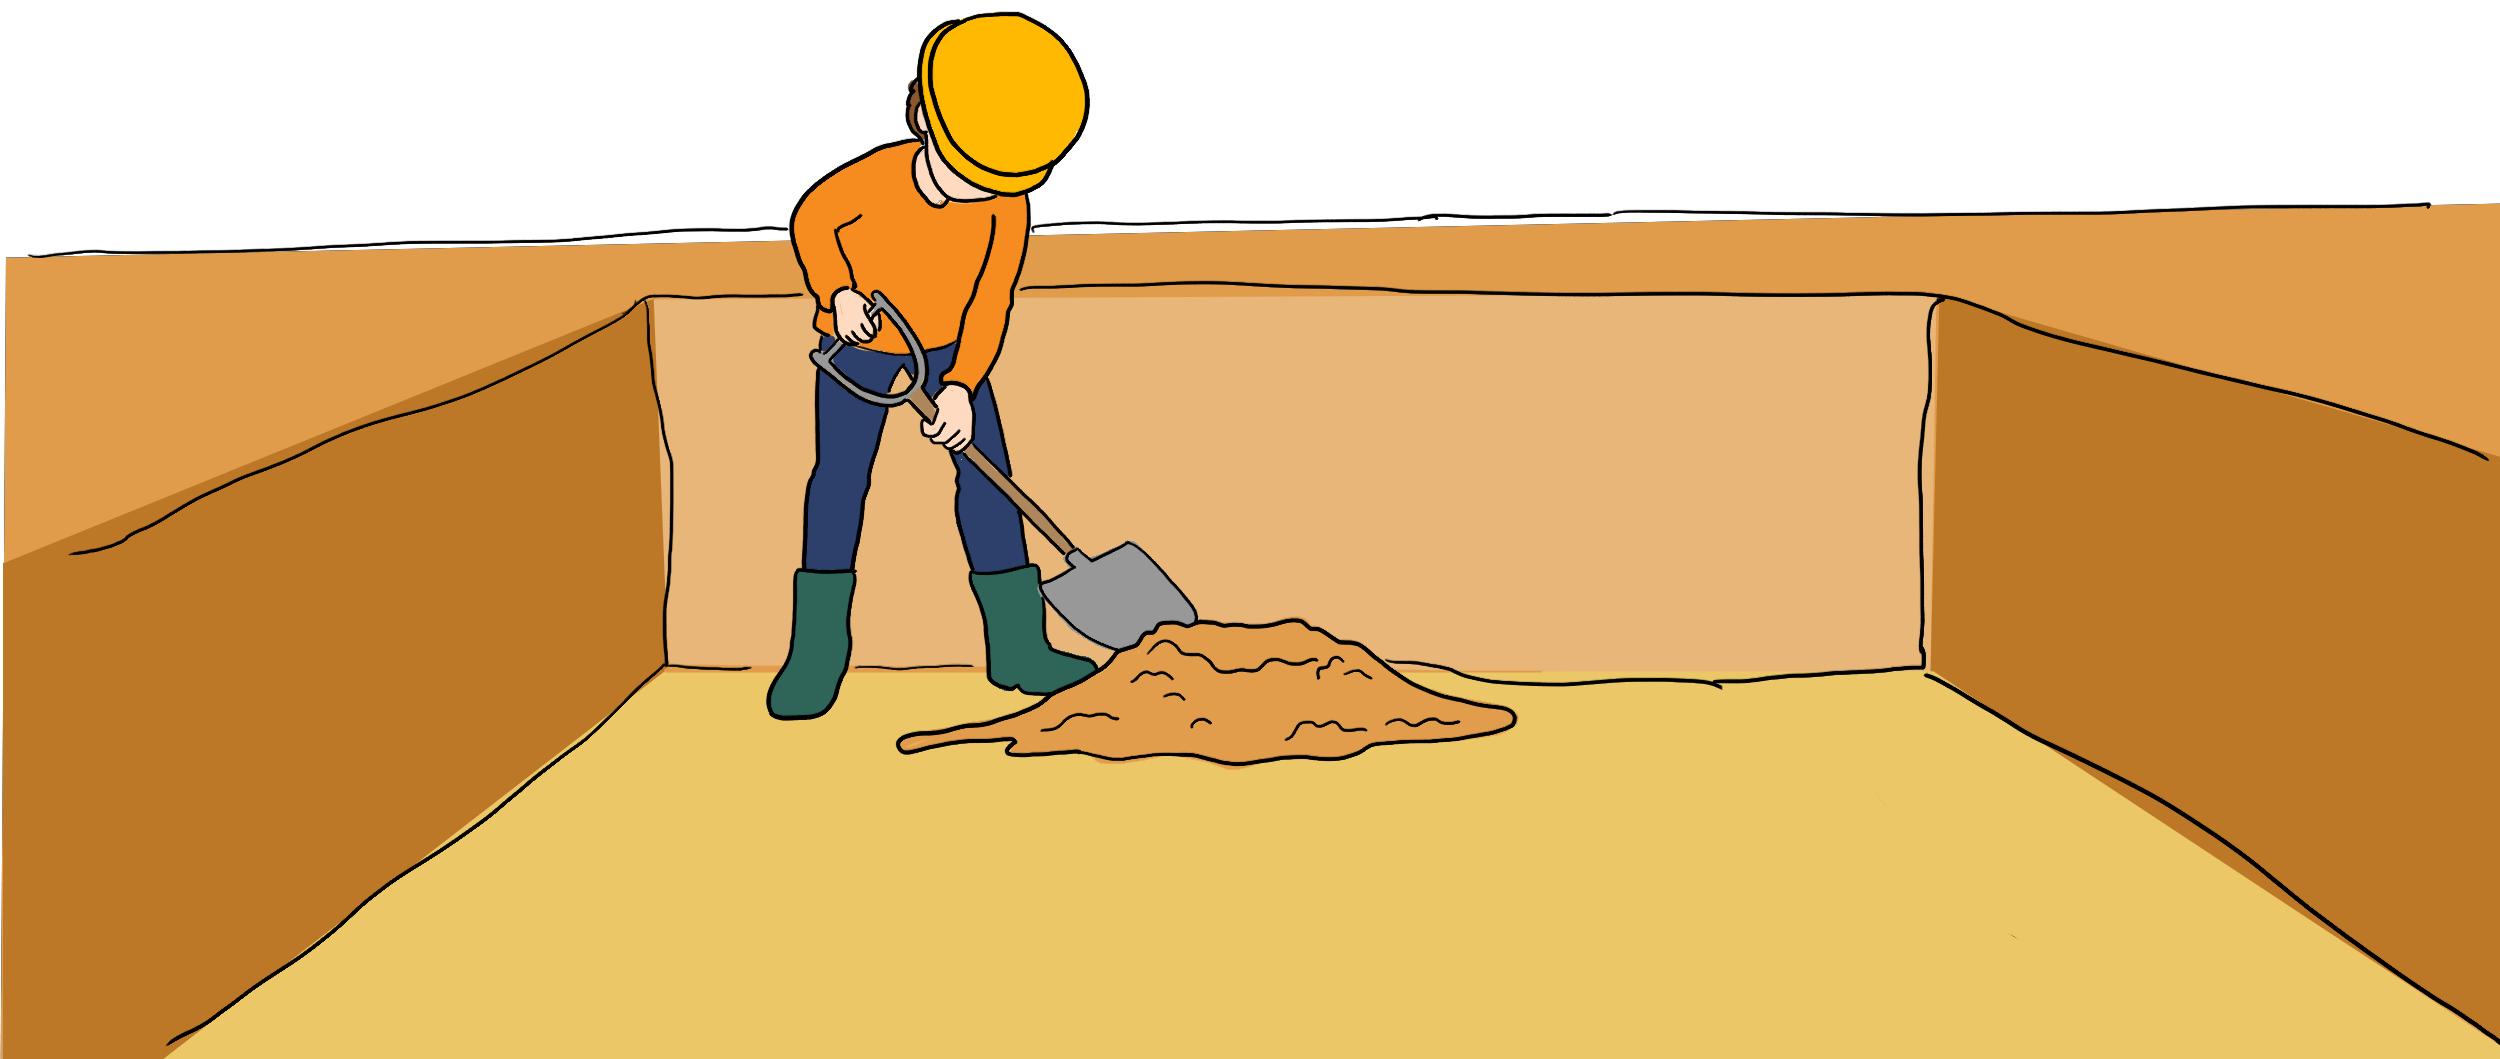
\includegraphics[width=1\linewidth]{Pi7_bai2}
%		\vspace*{-20pt}
%	\end{figure}
%	\textit{Lời giải.} 	Giả sử trong thời gian mỗi người đào ở chiếc hố ban đầu, hai người còn lại sẽ đi đào một chiếc hố bổ sung thêm khác. Như vậy khi kết thúc công việc, cùng với chiếc hố ban đầu, họ sẽ đào thêm được $3\cdot 0{.}5 = 1{.}5$ chiếc hố. Do đó, nếu cả ba người cùng làm công việc đào, thì trong cùng số thời gian như ban đầu, họ sẽ đào được $1+1{.}5=2{.}5$ (hố). Vậy, nếu cả ba người cùng đào thì họ sẽ làm nhanh hơn được $2{.}5$ lần so với cách đào luân phiên lần lượt như ban đầu.
%	\vskip 0.1cm
%	$\pmb{3.}$ Ba bạn Gấu, Thỏ và Mèo cùng quyết định xây một con đường từ nhà tới bờ suối với chiều dài $160m$. Các bạn thoả thuận sẽ đầu tư cho dự án mở đường quan trọng này với công sức đều như nhau. Cuối cùng khi dự án hoàn thành, hoá ra bạn Thỏ đã xây được $60$ mét đường, bạn Mèo xây được $100$ mét đường, còn bạn Gấu mải ngủ đông nên không xây được mét nào. Tuy nhiên, Gấu mang tới đóng góp bằng tiền cho dự án là $16$ triệu đồng từ số mật ong bán được của mình. Hỏi hai bạn Mèo và bạn Thỏ cần phải phân chia số tiền cho nhau như thế nào?
%	\begin{figure}[H]
%		\centering
%		\vspace*{-5pt}
%		\captionsetup{labelformat= empty, justification=centering}
%		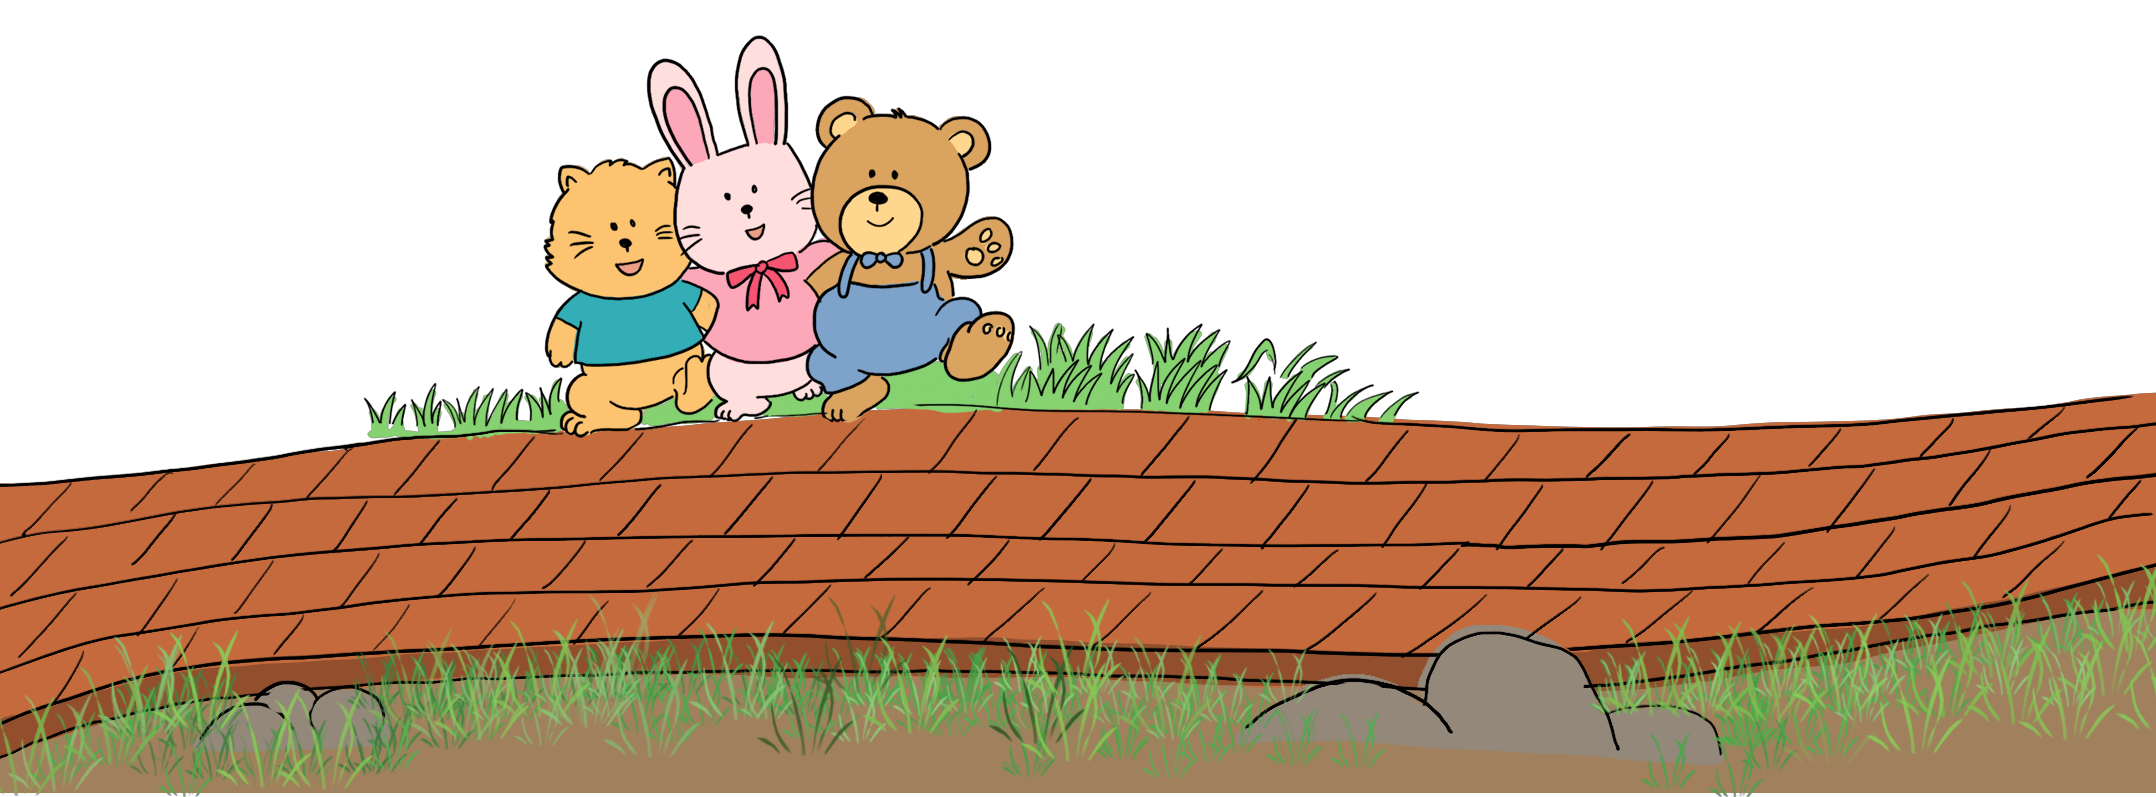
\includegraphics[width=1\linewidth]{Pi7_bai3}
%		\vspace*{-15pt}
%	\end{figure}
%	\textit{Lời giải.} 	Mỗi bạn theo kế hoạch phải xây đúng $\dfrac{160}{3} = 53\dfrac{1}{3}$  mét đường. Thỏ xây được $60$ (m) và Gấu xây được $100$ (m). Như vậy bạn Thỏ đã xây thay cho bạn Gấu số mét đường là
%	\begin{align*}
%		60 - 53 \frac{1}{3} = 6 \frac{2}{3}= \frac{20}{3} \text{ (m)},
%	\end{align*}
%	còn bạn Mèo đã xây thay cho bạn Gấu số mét đường
%	\begin{align*}
%		100- 53 \frac{1}{3} = 46 \frac{2}{3}=\frac{140}{3} \text{ (m).}
%	\end{align*}
%	Vì vậy số tiền mà bạn Gấu mang tới phải chia cho Thỏ và Mèo theo tỷ lệ $2: 14$, tức là Mèo được $14$ triệu đồng, còn Thỏ được $2$ triệu đồng từ số tiền đóng góp công sức của Gấu.
%	\vskip 0.1cm
%	$\pmb{4.}$ Bé Ly phải đi trồng hoa vào một hàng các chậu rất dài đặt thành hàng dọc ở công viên. Bé được giao nhiệm vụ là phải trồng hai loại hoa khác nhau vào hai chiếc chậu nếu giữa hai chậu này có đúng hai chiếc chậu, hoặc đúng ba chiếc chậu, hoặc đúng năm chiếc chậu khác. Hỏi bé Ly phải cần ít nhất bao nhiêu loại hoa để thực hiện được nhiệm vụ?
%	\begin{figure}[H]
%		\centering
%		\vspace*{-5pt}
%		\captionsetup{labelformat= empty, justification=centering}
%		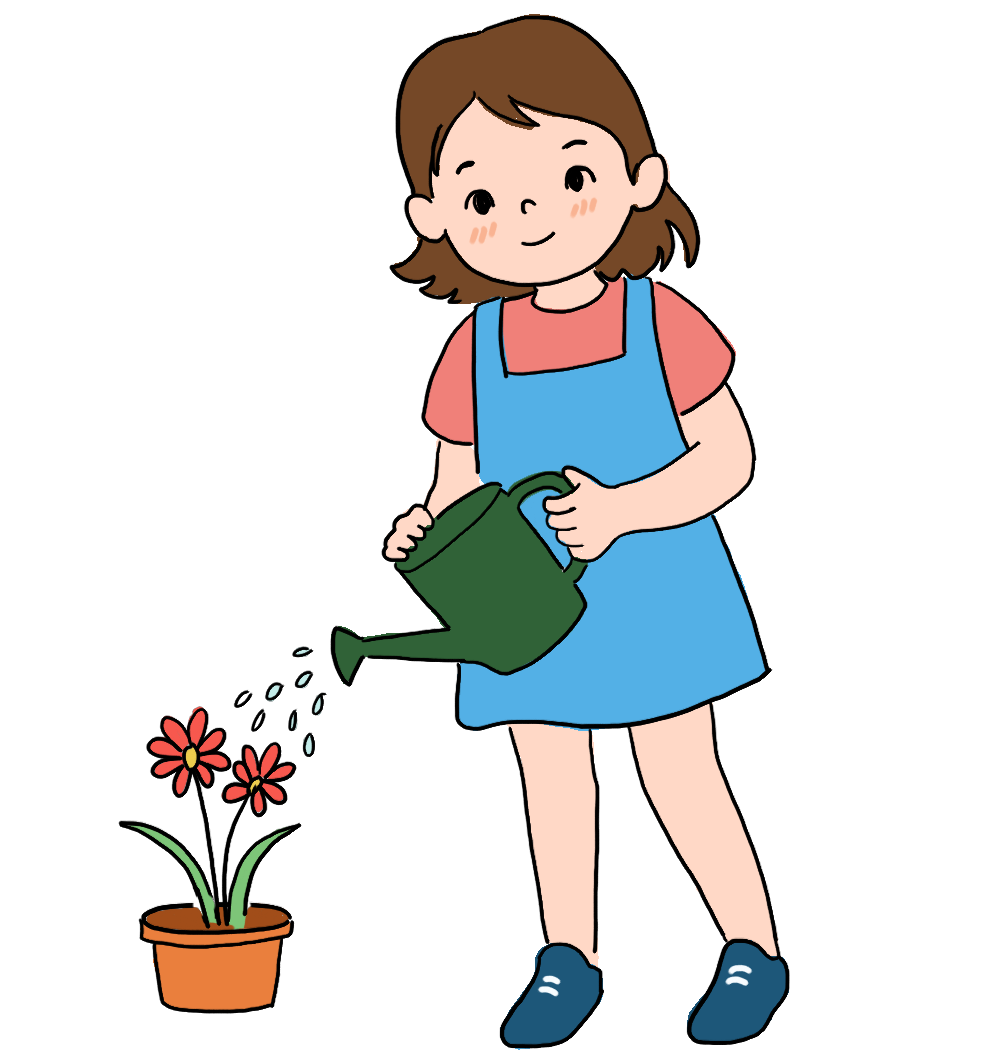
\includegraphics[width=0.45\linewidth]{Pi7_bai4}
%		\vspace*{-10pt}
%	\end{figure}
%	\textit{Lời giải.} Trước tiên ta thấy rằng bé Ly có thể chỉ cần $3$ loại hoa là thực hiện được nhiệm vụ. Thật vậy, giả sử Ly có $3$ loại là $A, B, C$. Khi đó nếu Ly trồng $3$ chậu đầu tiên trong hàng bằng loại $A$, $3$ chậu tiếp theo bằng loại $B$, $3$ chậu tiếp loại $C$ và lại $3$ chậu tiếp theo quay lại bằng loại $A$, vv \ldots thì rõ ràng yêu cầu đặt ra được thực hiện. 
%	\vskip 0.1cm
%	Bây giờ giả sử Ly chỉ có $2$ loại hoa là $A$ và $B$. Nếu Ly trồng ở chậu thứ nhất bằng hoa loại $A$ (không mất tính tổng quát), suy ra các chậu có số thứ tự tiếp theo là $4, 5, 7$ phải được trồng bằng hoa loại $B$. Nhưng khi đó giữa hai chậu số $4$ và số $7$ đều được trồng cùng loại hoa $B$ nhưng giữa chúng có đúng hai chậu khác là số $5$ và số $6$, suy ra mâu thuẫn với yêu cầu.
%	\vskip 0.1cm
%	Vậy Ly cần ít nhất $3$ loại hoa để trồng theo yêu cầu đặt ra.
%	 \vskip 0.1cm
%	$\pmb{5.}$ Trước một trận bóng đá giữa hai đội Xóm Đông và Xóm Bắc có $5$ dự đoán kết quả được đưa ra:
%	\vskip 0.1cm
%	$a)$	Sẽ không có tỷ số hoà;
%	\vskip 0.1cm
%	$b)$	Đội Xóm Đông sẽ bị thủng lưới;
%	\vskip 0.1cm
%	$c)$	Đội Xóm Bắc sẽ thắng;
%	\vskip 0.1cm
%	$d)$	Đội Xóm Bắc sẽ không thua;
%	\vskip 0.1cm
%	$e)$	Trong trận bóng sẽ có đúng $3$ bàn thắng được ghi.
%	\vskip 0.1cm
%	Sau khi trận bóng kết thúc, hoá ra chỉ có đúng $3$ dự đoán là chính xác. Vậy trận đấu đã kết thúc với tỷ số như thế nào?
%	\begin{figure}[H]
%		\centering
%%		\vspace*{-5pt}
%		\captionsetup{labelformat= empty, justification=centering}
%		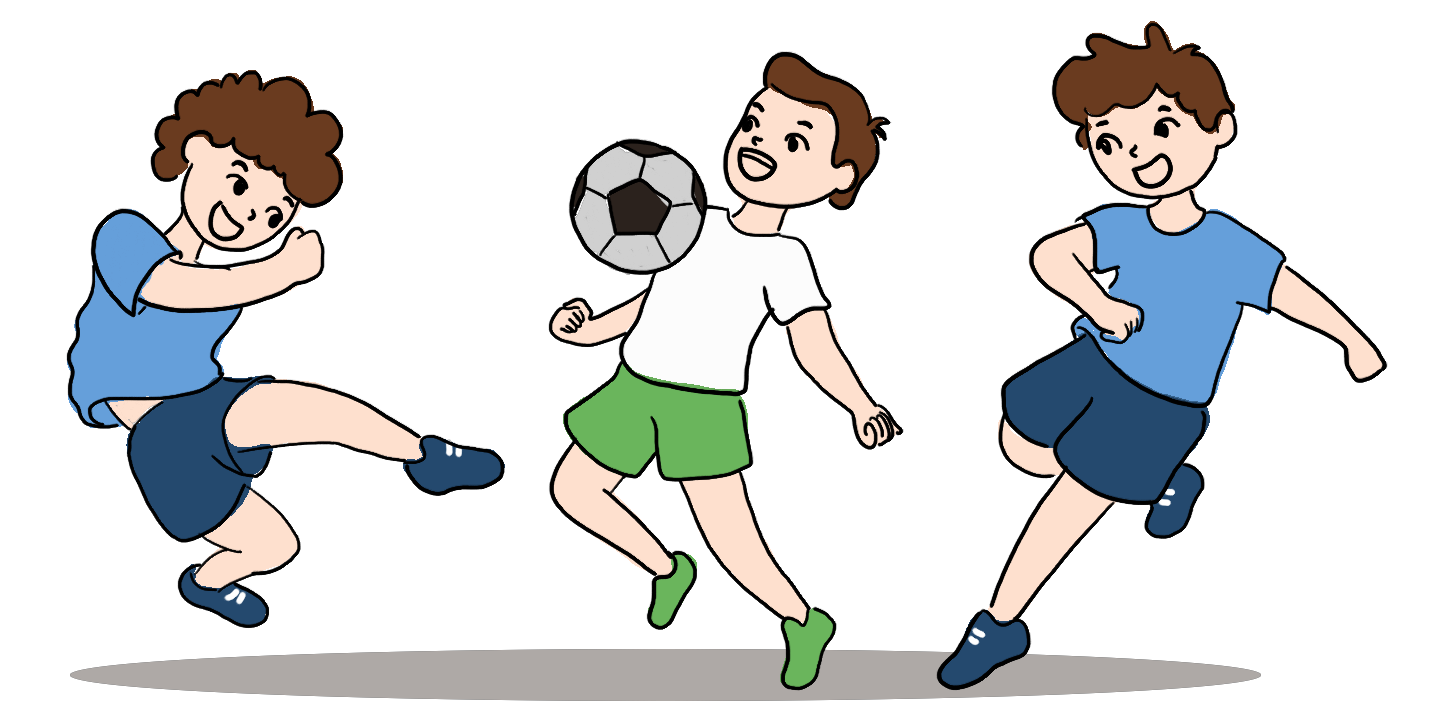
\includegraphics[width=0.85\linewidth]{Pi7_bai5}
%		\vspace*{-10pt}
%	\end{figure}
%	\textit{Lời giải.} Giả sử là đội Xóm Bắc thắng. Khi đó $4$ dự đoán $a)$, $b)$ $c)$ và $d)$ đều đúng, mâu thuẫn với điều kiện đặt ra.
%	\vskip 0.1cm
%	Tiếp theo, giả sử trận đấu kết thúc với tỷ số hoà. Khi đó ta lại có các dự đoán $a)$, $c)$ và $e)$ đều sai, điều này cũng mâu thuẫn với điều kiện đã cho.
%	\vskip 0.1cm
%	Vì vậy, trong trận bóng này đội Xóm Bắc đã thua. Khi đó các dự đoán $c)$ và $d)$ đều sai, và $3$ dự đoán còn lại là đúng. Có nghĩa là: trận đấu không có tỷ số hoà, có ít nhất một trái bóng được đưa vào lưới của đội Xóm Đông, và trong trận bóng có đúng $3$ bàn thắng được ghi. Điều đó có nghĩa là trận bóng kết thúc với tỷ số $1:2$ nghiêng về phía đội Xóm Đông.
%	\vskip 0.1cm
%	$\pmb{6.}$ 	Tại trại hè có $20$ em học sinh tham gia trò chơi Điệp viên tí hon diễn ra trong $2$ tuần. Mỗi Điệp viên tí hon sẽ theo dõi và viết báo cáo tỉ mỉ về sở thích cá nhân của $10$ em khác trong số $20$ em này để nộp cho Sở chỉ huy. Em hãy chứng tỏ rằng có ít nhất $10$ cặp Điệp viên tí hon đã theo dõi lẫn nhau và viết báo cáo về nhau.
%	\begin{figure}[H]
%		\centering
%		\vspace*{-5pt}
%		\captionsetup{labelformat= empty, justification=centering}
%		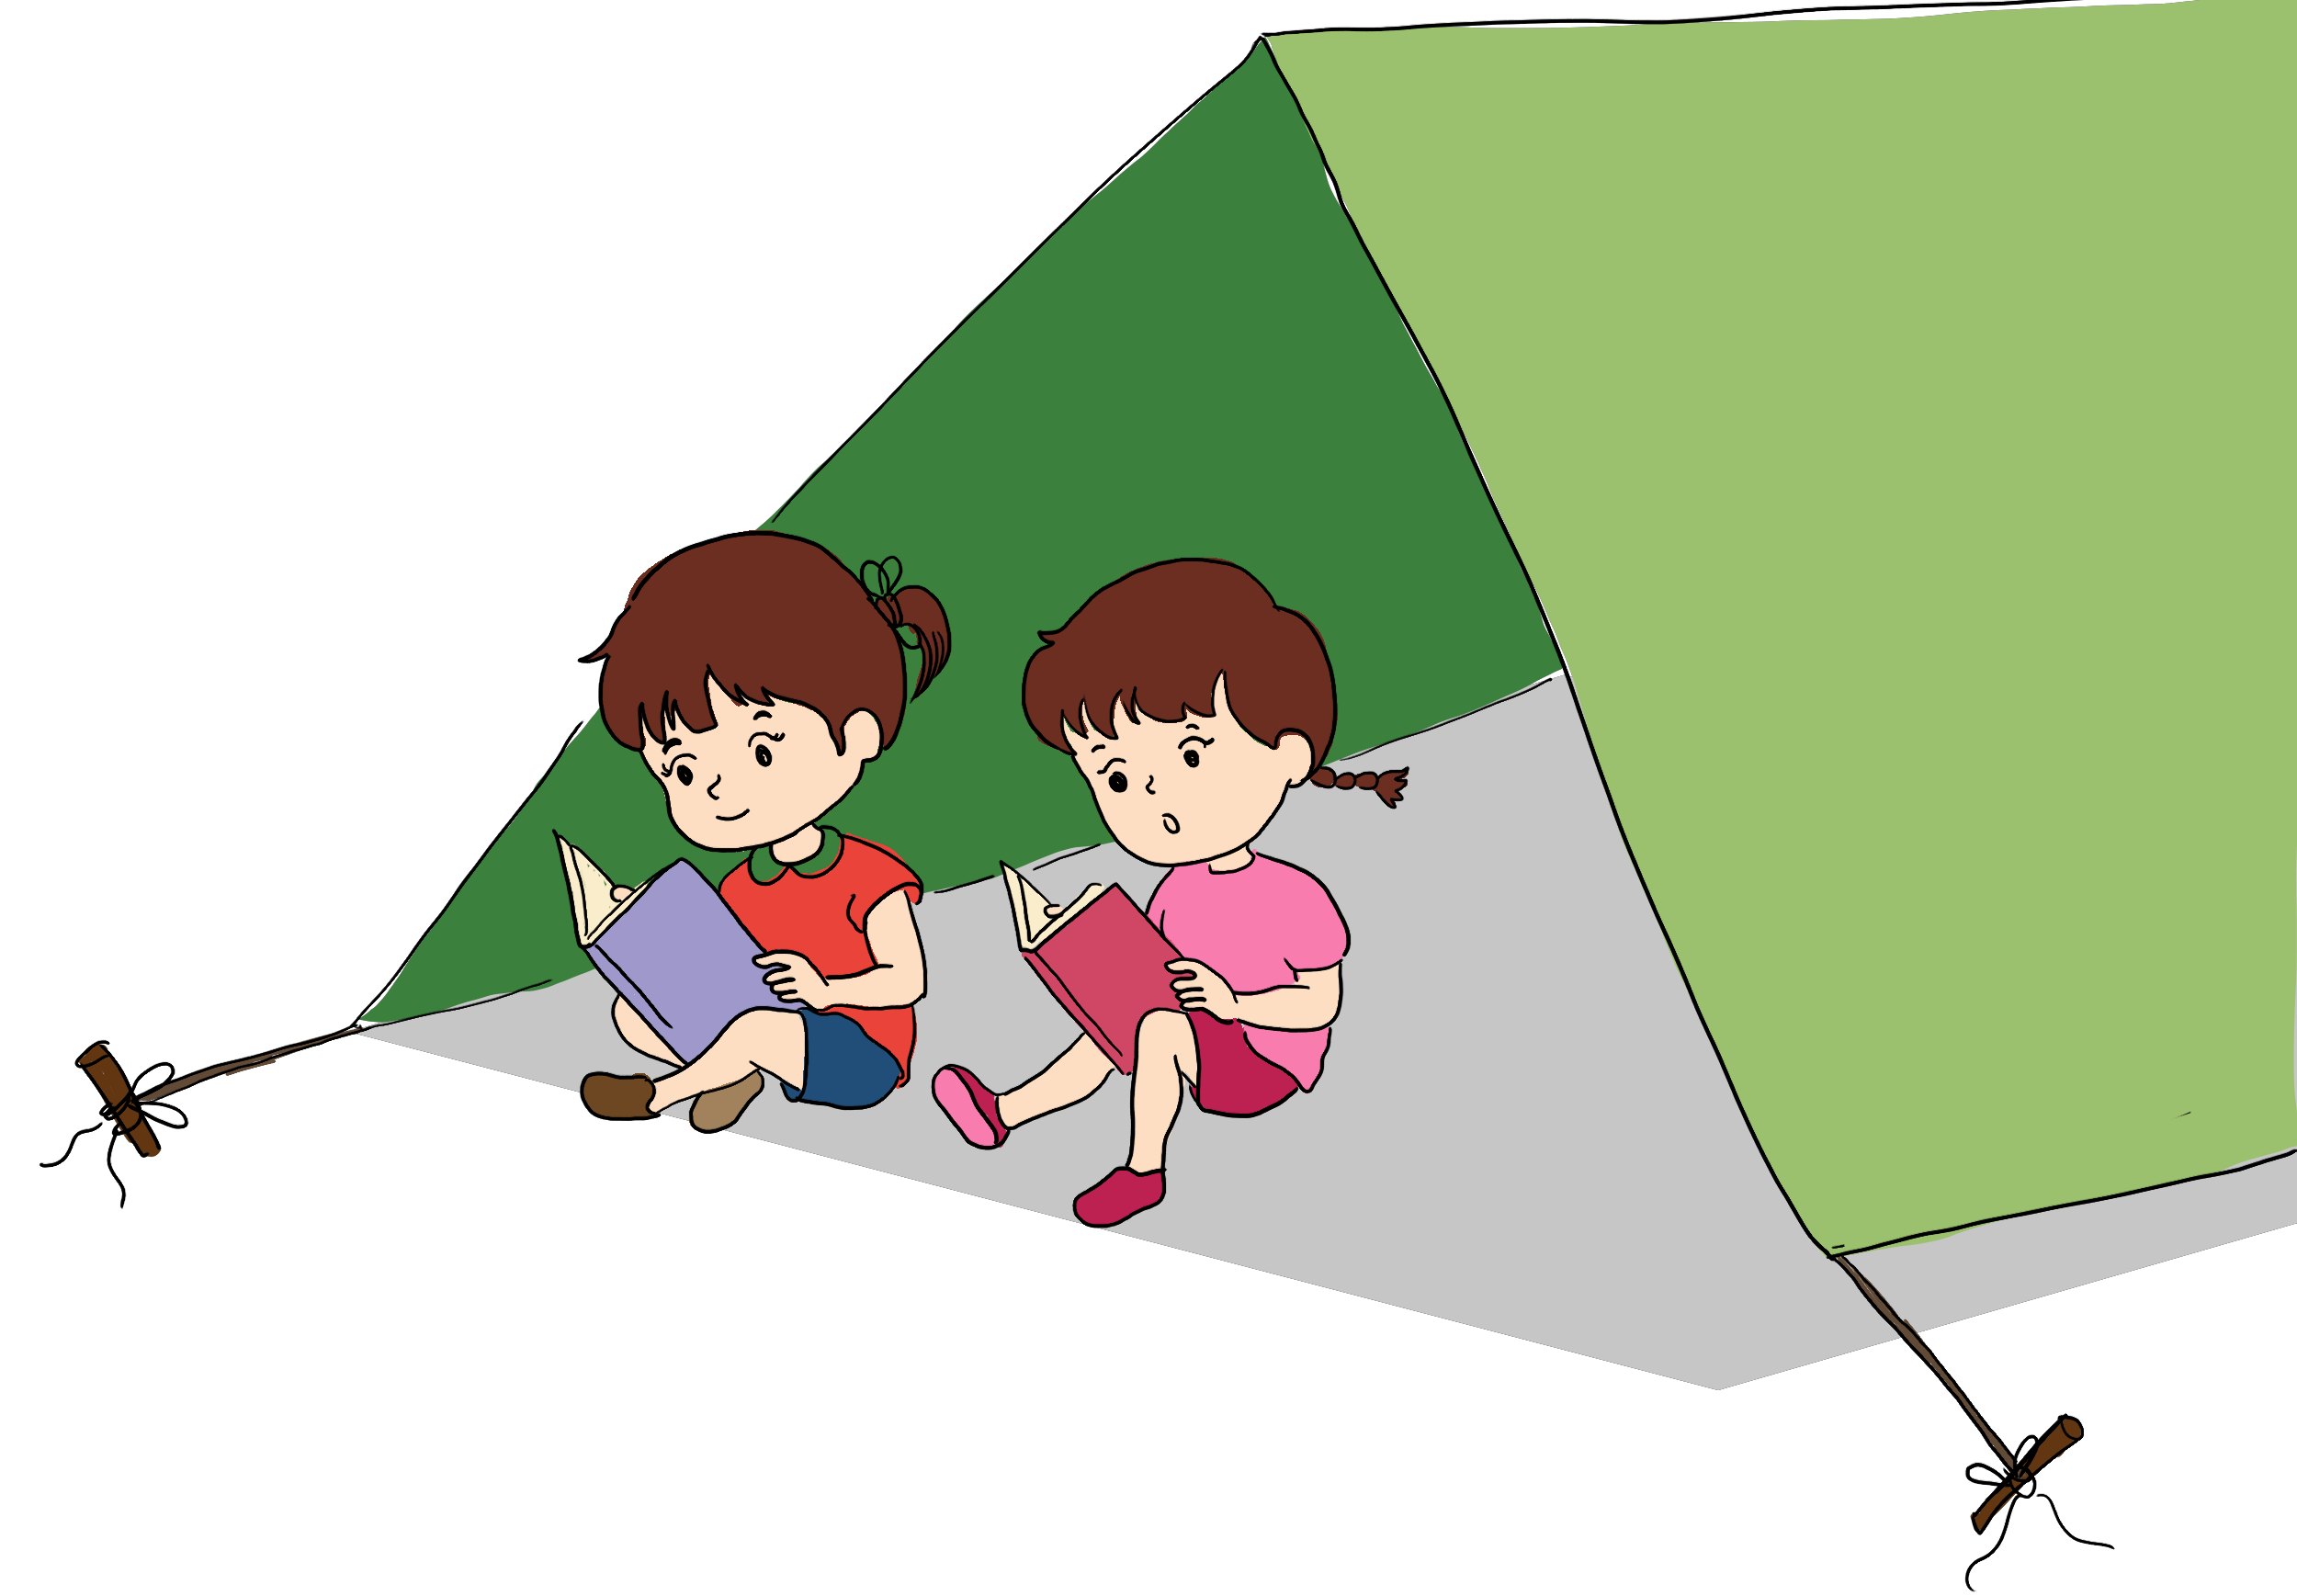
\includegraphics[width=0.75\linewidth]{Pi7_bai6}
%		\vspace*{-15pt}
%	\end{figure}
%	\textit{Lời giải.} Số các cặp Điệp viên tí hon là $\dfrac{20\times 19}{2} = 190$ (cặp). Có tất cả $10\times 20=200$ báo cáo được gửi về Sở chỉ huy vào cuối đợt chơi, suy ra phải có ít nhất $10$ cặp Điệp viên mà hai người trong mỗi cặp báo cáo lẫn nhau về Sở chỉ huy.
%\end{multicols}
%
\newpage
\graphicspath{{../toancuabi/toantienganh/}}
\begingroup
\thispagestyle{toancuabinone}
\blfootnote{$^1$\color{toancuabi}Ottawa, Canada.}
\AddToShipoutPicture*{\put(60,733){
\includegraphics[width=17.2cm]{../mathc.pdf}}}
%\AddToShipoutPicture*{\put(-2,733){
\includegraphics[width=17.2cm]{../mathl.pdf}}} 
\AddToShipoutPicture*{\put(106,675){
\includegraphics[scale=1]{../tieudeb.pdf}}} 
\centering
\endgroup
\vspace*{35pt}

\begin{multicols}{2}
	\setlength{\abovedisplayskip}{6pt}
	\setlength{\belowdisplayskip}{6pt}
	In this article, we will investigate a number of ways to \textit{prove area equality without writing lengthy proof.}
	While it sounds simple, easy, and exciting, it is important that you need to improve your creating thinking in order to 
	first understand the examples, and then use them as tools, guidelines, or ideas to solve the problems.
	\vskip 0.2cm
	\PIbox{
	\textbf{\color{toancuabi}Example $\pmb1$.}
	$E$ is an arbitrary point inside the parallelogram $ABCD,$ prove that
	\begin{align*}
		[AEB] + [CED] = \half [ABCD].
	\end{align*}}
	\begin{figure}[H]
		\vspace*{-5pt}
		\centering
		\captionsetup{labelformat= empty, justification=centering}
		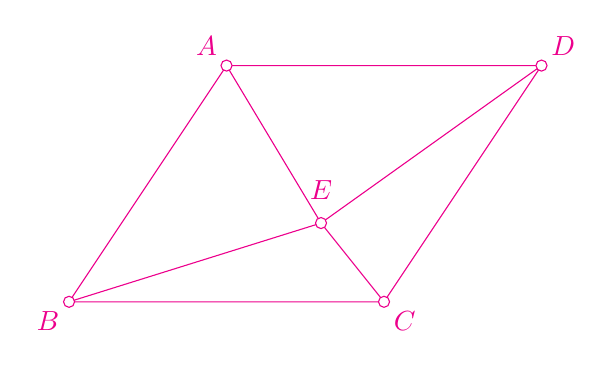
\begin{tikzpicture}[toancuabi]
			\draw (0,0) -- (4,0) -- (6,3) -- (2,3) -- (0,0) -- (3.2,1) -- (4,0) (2,3) -- (3.2,1) -- (6,3);
			\draw[fill=white] (3.2,1) circle (2pt) node [above=5pt] {$E$};
			\draw[fill=white] (2,3) circle (2pt) node [anchor = south east] {$A$};
			\draw[fill=white] (0,0) circle (2pt) node [anchor = north east] {$B$};
			\draw[fill=white] (4,0) circle (2pt) node [anchor = north west] {$C$};
			\draw[fill=white] (6,3) circle (2pt) node [anchor = south west] {$D$};
		\end{tikzpicture}
		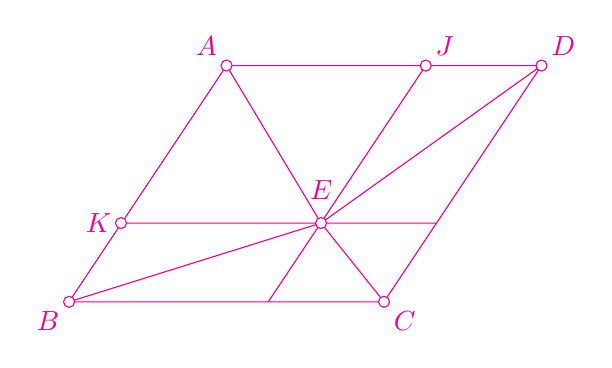
\begin{tikzpicture}[toancuabi]
			\draw (0,0) -- (4,0) -- (6,3) -- (2,3) -- (0,0) -- (3.2,1) -- (4,0) (2,3) -- (3.2,1) -- (6,3) (2.53,0) -- (4.53,3) (0.66,1) --(4.66,1);
			\draw[fill=white] (3.2,1) circle (2pt) node [above=5pt] {$E$};
			\draw[fill=white] (2,3) circle (2pt) node [anchor = south east] {$A$};
			\draw[fill=white] (0,0) circle (2pt) node [anchor = north east] {$B$};
			\draw[fill=white] (4,0) circle (2pt) node [anchor = north west] {$C$};
			\draw[fill=white] (6,3) circle (2pt) node [anchor = south west] {$D$};
			\draw[fill=white] (4.53,3) circle (2pt) node [anchor = south west] {$J$};
			\draw[fill=white] (0.66,1) circle (2pt) node [left] {$K$};
		\end{tikzpicture}
		\vspace*{-10pt}
	\end{figure}
%	\begin{figure}[H]
%		\vspace*{-10pt}
%		\centering
%		\captionsetup{labelformat= empty, justification=centering}
%		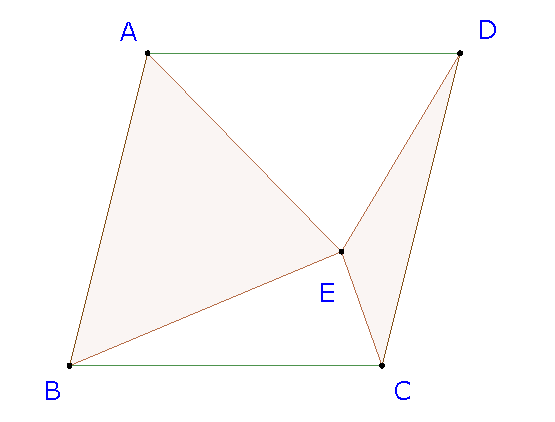
\includegraphics[width= 1\linewidth]{23-24-s3-i-p1.pdf}
%		\vspace*{-20pt}
%	\end{figure}
	\textit{Solution.}
	Draw lines through $E,$ parallel with sides of $ABCD,$ dividing the parallelogram into four smaller parallelograms.
	Any of the smaller parallelogram, say $AKEJ$, consists of a brown triangle from the shaded triangle and a green triangles with the same area.
	Thus, the area of the shaded triangles is the sum of the area of all smaller brown triangles, which is half of the sum of the area of all smaller parallelograms,
	of half of the $ABCD$ parallelogram.
	\vskip 0.1cm
	\textbf{\color{toancuabi}Remark.} Here's how we use the techniques:
	\vskip 0.1cm
	$1.$ First, divide the given figure into smaller figures.
	\vskip 0.1cm
	$3$. Deal with each of them, iif they have the same shape, then work in the same way.
	\vskip 0.1cm
	$3.$ Use all partial results to arrive at the overall result.
	\vskip 0.2cm
%	\begin{figure}[H]
%		\vspace*{-5pt}
%		\centering
%		\captionsetup{labelformat= empty, justification=centering}
%		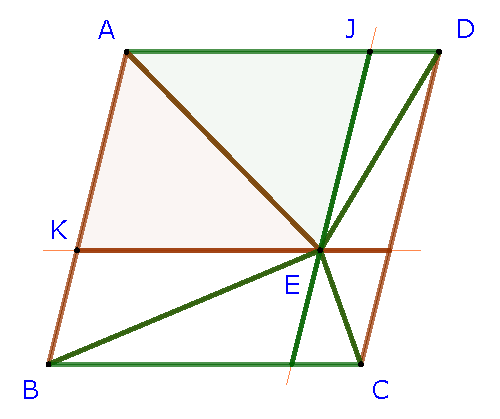
\includegraphics[width= 0.9\linewidth]{23-24-s3-i-p1-s.pdf}
%		\vspace*{-15pt}
%	\end{figure}
	\PIbox{\textbf{\color{toancuabi}Example $\pmb2$.}
	$E$ and $F$ are midpoints of $BC$ and $DA$ in the convex quadrilateral $ABCD,$ prove that
	\begin{align*}
		[AECF] = \half [ABCD].
	\end{align*}}
\begin{figure}[H]
	\vspace*{-5pt}
	\centering
	\captionsetup{labelformat= empty, justification=centering}
	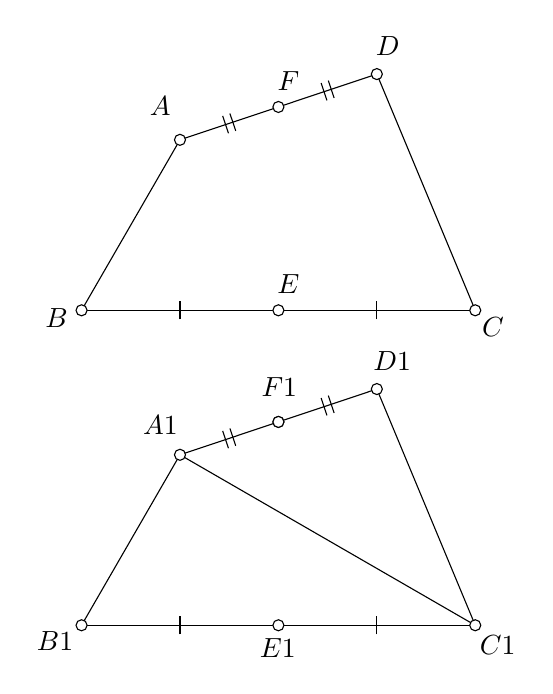
\begin{tikzpicture}
		\draw  (5.,0.)-- (3.75,3.);
		\draw  (5.,-4.)-- (3.75,-1.);
		\draw  (0.,0.)-- (1.25,2.165063509461097);
		\draw  (1.25,2.165063509461097)-- (2.5,2.5825317547305486);
		\draw  (1.7922093978532345,2.468742834111641) -- (1.8658796296660776,2.248156500157986);
		\draw  (1.884120370333924,2.499438764033659) -- (1.957790602146767,2.278852430080004);
		\draw  (2.5,2.5825317547305486)-- (3.75,3.);
		\draw  (3.0422093978532336,2.8862110793810927) -- (3.1158796296660767,2.6656247454274378);
		\draw  (3.134120370333923,2.9169070093031104) -- (3.207790602146766,2.6963206753494555);
		\draw  (5.,-4.)-- (2.5,-4.);
		\draw  (3.75,-4.11628159117254) -- (3.75,-3.8837184088274594);
		\draw  (2.5,-4.)-- (0.,-4.);
		\draw  (1.25,-4.11628159117254) -- (1.25,-3.8837184088274594);
		\draw  (0.,-4.)-- (1.25,-1.8349364905389032);
		\draw  (1.25,-1.8349364905389032)-- (5.,-4.);
		\draw  (5.,0.)-- (2.5,0.);
		\draw  (3.75,-0.11628159117254047) -- (3.75,0.11628159117254047);
		\draw  (2.5,0.)-- (0.,0.);
		\draw  (1.25,-0.11628159117254047) -- (1.25,0.11628159117254047);
		\draw  (1.25,-1.8349364905389032)-- (2.5,-1.4174682452694516);
		\draw  (1.7922093978532345,-1.53125716588836) -- (1.8658796296660776,-1.7518434998420143);
		\draw  (1.884120370333924,-1.5005612359663414) -- (1.957790602146767,-1.7211475699199956);
		\draw  (2.5,-1.4174682452694516)-- (3.75,-1.);
		\draw  (3.0422093978532336,-1.1137889206189073) -- (3.1158796296660767,-1.3343752545725616);
		\draw  (3.134120370333923,-1.0830929906968887) -- (3.207790602146766,-1.303679324650543);
			\draw [fill=white] (0.,0.) circle (2.0pt);
			\draw (-0.3177952991732108,-0.09743478291470092) node {$B$};
			\draw [fill=white] (5.,0.) circle (2.0pt);
			\draw (5.224960546717885,-0.21371637408724142) node {$C$};
			\draw [fill=white] (2.5,0.) circle (2.0pt);
			\draw (2.6280050105311474,0.3289310513846141) node {$E$};
			\draw [fill=white] (1.25,2.165063509461097) circle (2.0pt);
			\draw (1.0000627341155812,2.5964220792491535) node {$A$};
			\draw [fill=white] (3.75,3.) circle (2.0pt);
			\draw (3.8877222482336693,3.3522524218706664) node {$D$};
			\draw [fill=white] (2.5,2.5825317547305486) circle (2.0pt);
			\draw (2.6280050105311474,2.906506322375928) node {$F$};
			\draw [fill=white] (0.,-4.) circle (2.0pt);
			\draw (-0.33717556436863416,-4.206051004344464) node {$B1$};
			\draw [fill=white] (5.,-4.) circle (2.0pt);
			\draw (5.283101342304154,-4.244811534735311) node {$C1$};
			\draw [fill=white] (3.75,-1.) circle (2.0pt);
			\draw (3.94586304381994,-0.6400822083865565) node {$D1$};
			\draw [fill=white] (2.5,-4.) circle (2.0pt);
			\draw (2.492343154163184,-4.283572065126157) node {$E1$};
			\draw [fill=white] (1.25,-1.8349364905389032) circle (2.0pt);
			\draw (1.0000627341155812,-1.4540533465943397) node {$A1$};
			\draw [fill=white] (2.5,-1.4174682452694516) circle (2.0pt);
			\draw (2.5117234193586073,-0.9695467167087544) node {$F1$};
			\draw [fill=white] (2.5,-1.4174682452694516) circle (2.0pt);
	\end{tikzpicture}
	\vspace*{-10pt}
\end{figure}

	\textit{Solution.}
	Connect $AC.$ Since $E$ is midpoint of $BC,$ thus the triangles $ABE$ and $AEC$ have the same area.
	Similarly triangles $CDF$ and $CFA$ have the same area. Thus the area of $AECF$ is half of $ABCD.$
	\vskip 0.2cm
%	\begin{figure}[H]
%		\vspace*{-5pt}
%		\centering
%		\captionsetup{labelformat= empty, justification=centering}
%		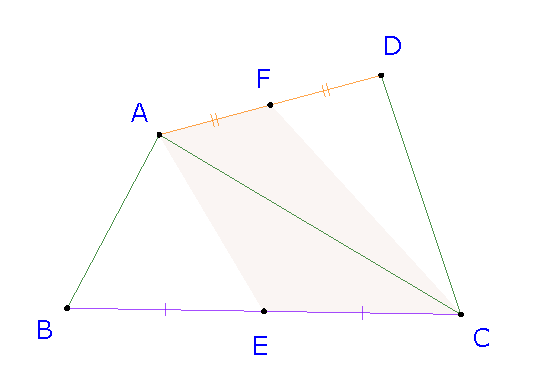
\includegraphics[width= 1\linewidth]{23-24-s3-i-p2-s.pdf}
%		\vspace*{-10pt}
%	\end{figure}
	\PIbox{\textbf{\color{toancuabi}Example $\pmb3$.}
		$I$ is an arbitrary point on the diagonal $BD$ in parallelogram $ABCD.$
		Lines through $I$ parallel with the sides of $ABCD$ intersect $AB,$ $BC,$ $CD,$ and $DA$ at $E, F, G,$ and $H,$ respectively.
		\begin{align*}
			[AEIH] = [FCGI].
		\end{align*}}
	\begin{figure}[H]
		\vspace*{-5pt}
		\centering
		\captionsetup{labelformat= empty, justification=centering}
		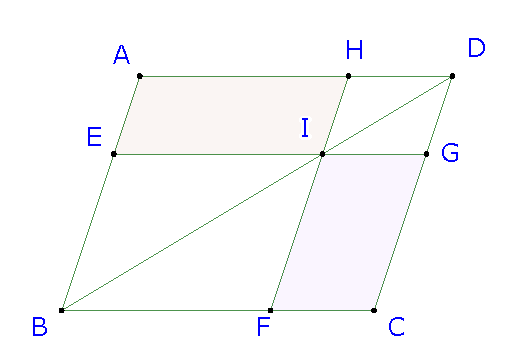
\includegraphics[width= 1\linewidth]{23-24-s3-i-p3.pdf}
		\vspace*{-10pt}
	\end{figure}
	\textit{Solution.}
	First, since $BD$ is the diagonal in parallelogram $ABCD,$ $[ABD] = [BCD].$
	Now, $BEIF$ is also a parallelogram, thus $[BEI] = [BFI],$ similarly $[HID] = [IGD].$
	Therefore 
	\begin{align*}
		[AEIH] &= [ABD] - [BEI] - [HID] \\
		&= [BCD] - [BFI] - [IGD] \\
		&= [FCGI].
	\end{align*}
	\begin{figure}[H]
		\vspace*{-5pt}
		\centering
		\captionsetup{labelformat= empty, justification=centering}
		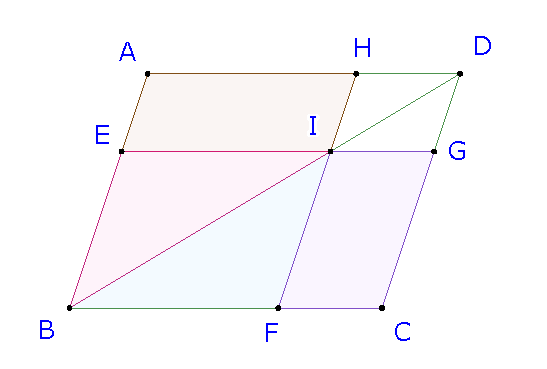
\includegraphics[width= 1\linewidth]{23-24-s3-i-p3-s.pdf}
		\vspace*{-10pt}
	\end{figure}
	\PIbox{\textbf{\color{toancuabi}Example $\pmb4$.} 
	$G, H$ are midpoints of $BC, CD$ in th regular hexagon $ABCDEF.$
	$EG$ and $FH$ intersect at $I.$ Prove that
	\begin{align*}
		[GCHI] = [EFI].
	\end{align*}}
	\begin{figure}[H]
		\vspace*{-5pt}
		\centering
		\captionsetup{labelformat= empty, justification=centering}
		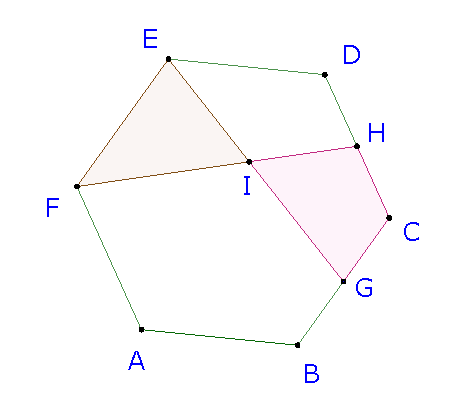
\includegraphics[width= 1\linewidth]{23-24-s3-i-p4.pdf}
		\vspace*{-10pt}
	\end{figure}
	\textit{Solution.}
		It is easy to see that the quadrilaterals $GCDE$ and $HDEF$ are congruent, thus have the same area, or $[GCDE] = [HDEF].$
		Taking $HDEI$ away, we have $[GCHI] = [EFI].$ 
	\vskip 0.2cm
	\PIbox{\textbf{\color{toancuabi}Example $\pmb5$.}
		$E, F, G,$ and $H$ are midpoints the sides in the convex quadrilateral $ABCD.$
		Prove that
		\begin{align*}
			[EFGH] = \half [ABCD].
		\end{align*}}
	\begin{figure}[H]
		\vspace*{-5pt}
		\centering
		\captionsetup{labelformat= empty, justification=centering}
		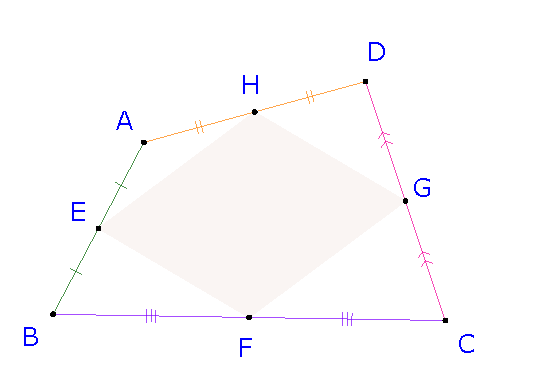
\includegraphics[width= 1\linewidth]{23-24-s3-i-p5.pdf}
		\vspace*{-10pt}
	\end{figure}
	\textit{Solution.}
		$EH$ is the mid-segment (the segment connecting two midpoints) in $\triangle ABD,$ therefore $[AEH] = \frac{1}{4}[ABD].$
		Similarly $[BEF] = \frac{1}{4}[ABC],$ $[CFG] = \frac{1}{4}[BCD],$ and $[GDH] = \frac{1}{4}[CDA],$ therefore:
		\begin{align*}
			&[AEH] + [BEF] + [CFG] + [GDH] \\
			&= \half [ABCD]\\
			 \Rightarrow  &[EFGH] = \half [ABCD].
		\end{align*} 
\end{multicols}

	\newpage 

	\setcounter{figure}{0}
	\thispagestyle{hoccungpinone}
\pagestyle{hoccungpi}
\everymath{\color{hoccungpi}}
\graphicspath{{../hoccungpi/pic/}}
\blfootnote{\color{hoccungpi}\color{hoccungpi}$^1$Giáo viên Toán trường THPT chuyên Lê Hồng Phong, Nam Định.}
\begingroup
\AddToShipoutPicture*{\put(0,616){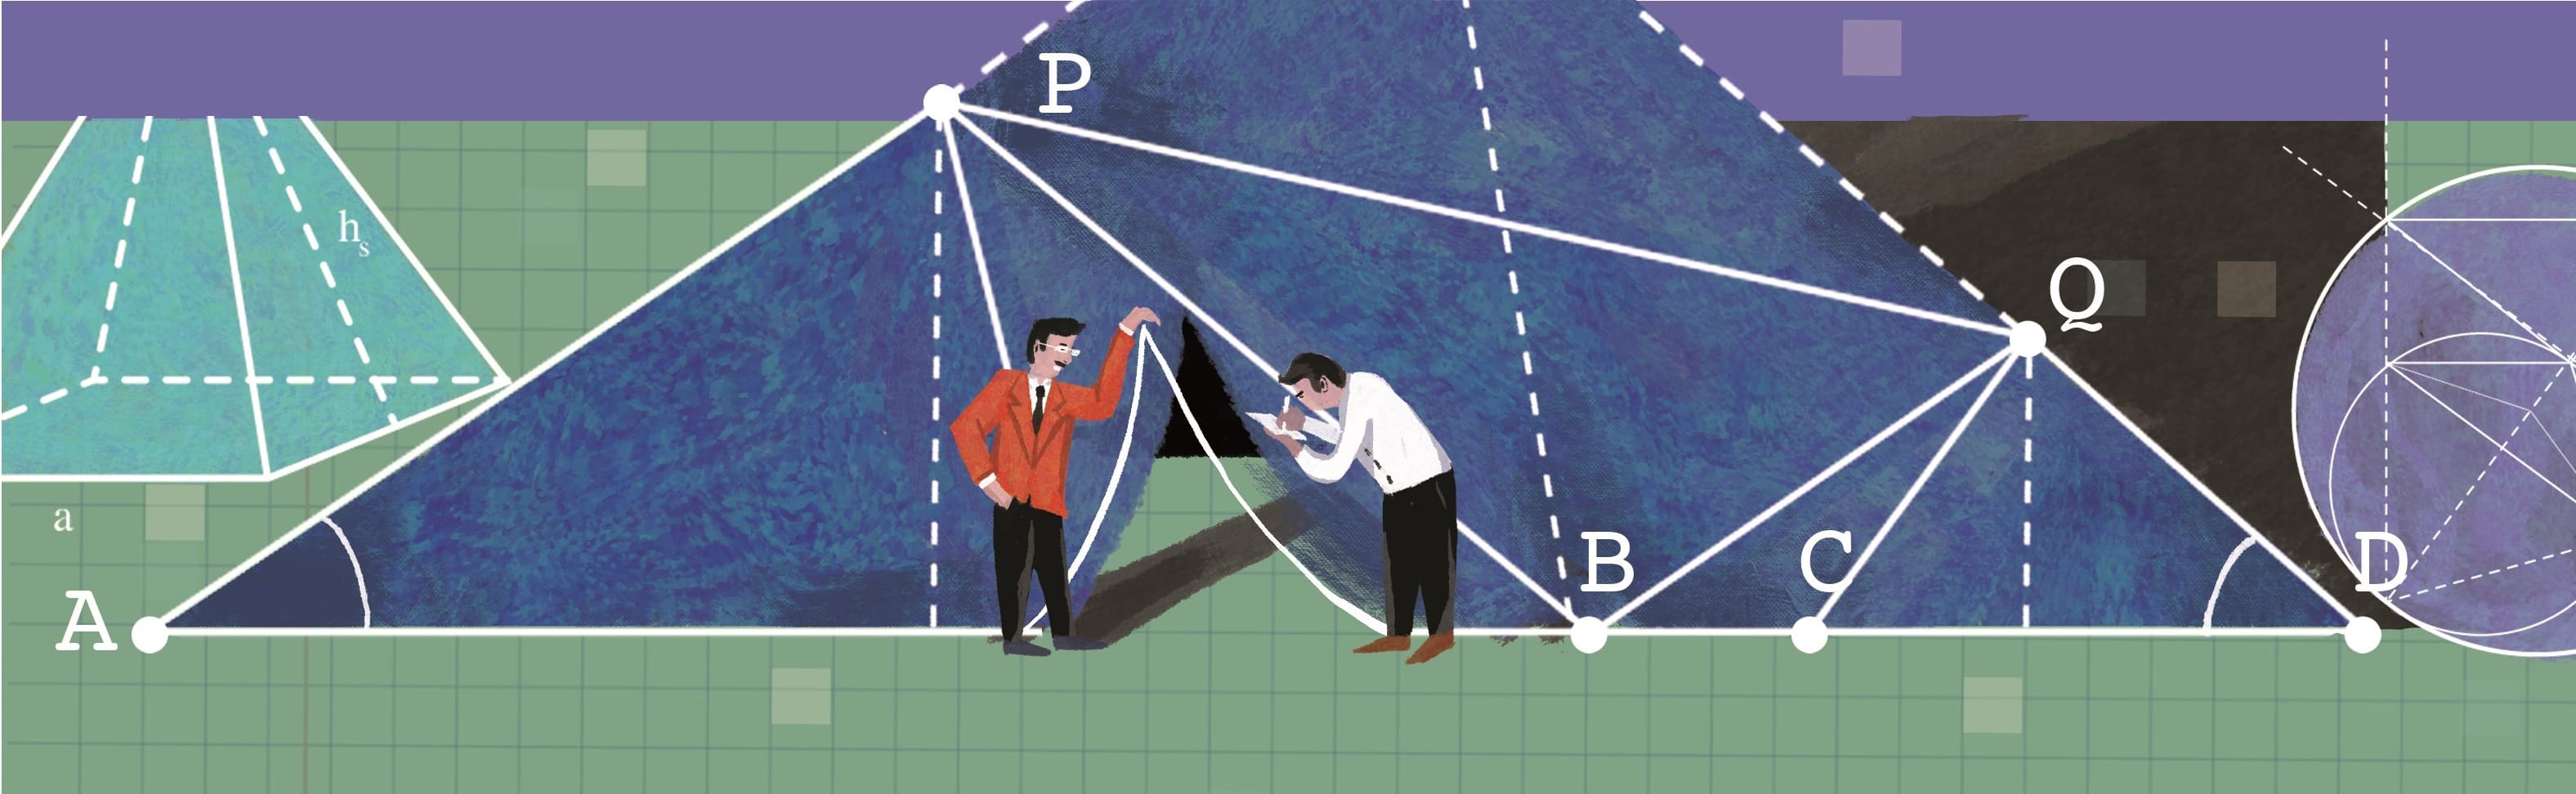
\includegraphics[width=19.3cm]{../bannerhoccungpi}}}
\AddToShipoutPicture*{\put(56,518){
\includegraphics[scale=1]{../tieude.pdf}}}
\centering
\endgroup
\vspace*{190pt}

\begin{multicols}{2}
	$\pmb{4.}$ \textbf{\color{hoccungpi}Đồ thị cây}
	\vskip 0.1cm
	Trong một số tình huống, ta có thể gặp những đồ thị mà số cạnh rất ít (còn gọi là đồ thị thưa). Khi đó, cấu trúc \textit{đồ thị cây} thường sẽ xuất hiện. Ta có định nghĩa về đồ thị cây như sau.
	\vskip 0.1cm
	\textbf{\color{hoccungpi}Định nghĩa} $\pmb{4.1}$ (Cây)\textbf{\color{hoccungpi}.}
	Một đồ thị được gọi là một \textit{cây} nếu nó liên thông và không chứa một chu trình nào. 
	\begin{figure}[H]
		\vspace*{-5pt}
		\centering
		\captionsetup{labelformat= empty, justification=centering}
		\definecolor{qqqqff}{rgb}{0.,0.,1.}
		\begin{tikzpicture}[scale=0.45, hoccungpi]
			\clip(3.52,0.5) rectangle (17.14,10.78);
			\draw  (9.,1.)-- (9.,4.);
			\draw  (9.,4.)-- (6.,7.);
			\draw  (6.,7.)-- (4.,10.);
			\draw  (6.,7.)-- (8.,10.);
			\draw  (9.,4.)-- (12.,10.);
			\draw  (9.,4.)-- (15.,7.);
			\draw  (15.,7.)-- (13.,10.);
			\draw  (15.,7.)-- (16.,10.);
			\begin{scriptsize}
				\draw [fill=qqqqff] (9.,1.) circle (5pt);
				\draw [fill=qqqqff] (9.,4.) circle (5pt);
				\draw [fill=qqqqff] (6.,7.) circle (5pt);
				\draw [fill=qqqqff] (4.,10.) circle (5pt);
				\draw [fill=qqqqff] (8.,10.) circle (5pt);
				\draw [fill=qqqqff] (12.,10.) circle (5pt);
				\draw [fill=qqqqff] (9.,4.) circle (5pt);
				\draw [fill=qqqqff] (15.,7.) circle (5pt);
				\draw [fill=qqqqff] (13.,10.) circle (5pt);
				\draw [fill=qqqqff] (16.,10.) circle (5pt);
			\end{scriptsize}
		\end{tikzpicture}
		\caption{\small\textit{\color{hoccungpi} Hình $5.$ Minh họa đồ thị cây.}}
		\vspace*{-10pt}
	\end{figure}
	Lưu ý rằng, một đồ thị cây không chứa chu trình, do đó nó không thể chứa một chu trình lẻ cạnh, hay một đồ thị cây cũng đồng thời là một đồ thị lưỡng phân. Nếu đồ thị $\pazocal{G}$ gồm một số thành phần liên thông, mà mỗi thành phần liên thông là một cây, thì $\pazocal{G}$ còn được gọi là một \textit{rừng}. Ta có định lý sau:
	\vskip 0.1cm 
	\textbf{\color{hoccungpi}Định lý} $\pmb{4.1}$ (Các đặc trưng tương đương của cây)\textbf{\color{hoccungpi}.}
	Cho  $\pazocal{G}$ là một đồ thị có $n$ đỉnh. Khi đó, các phát biểu sau là tương đương:
	\vskip 0.1cm
	$1.$ $\pazocal{G}$ là một cây;
	\vskip 0.1cm
	$2.$ $\pazocal{G}$ không có chu trình và có $n-1$ cạnh;
	\vskip 0.1cm
	$3.$ $\pazocal{G}$ liên thông và có $n-1$ cạnh;
	\vskip 0.1cm
	$4.$ $\pazocal{G}$ không có chu trình và nếu bổ sung vào một cạnh nối hai đỉnh không kề nhau thì xuất hiện một chu trình duy nhất;
	\vskip 0.1cm
	$5.$ $\pazocal{G}$ liên thông và nếu bỏ đi một cạnh bất kỳ thì $\pazocal{G}$ mất tính liên thông;
	\vskip 0.1cm
	$6.$ Mỗi cặp đỉnh trong $\pazocal{G}$ được nối với nhau bằng một đường đi duy nhất.
	\vskip 0.1cm
	Việc chứng minh định lý trên không khó. Bạn đọc quan tâm có thể tìm hiểu chi tiết chứng minh trong [$4$]. Để minh họa, chúng ta hãy cùng xét hai ví dụ sau.
	\vskip 0.1cm
	\textbf{\color{hoccungpi}Ví dụ} $\pmb{4.1}$ (Bài toán dự tuyển thi IMO  năm $2019$, Croatia đề xuất)\textbf{\color{hoccungpi}.}
	Trong một mạng xã hội, có $2019$ người dùng, một số họ là bạn của nhau (quan hệ bạn bè là quan hệ $2$ chiều). Ban đầu, có $1010$ người mà mỗi người có đúng $1009$ bạn và có $1009$ người mà mỗi người có đúng $1010$ bạn. Tuy nhiên, quan hệ bạn bè trong mạng này không bền vững, những sự kiện tương tự như sự kiện sau có thể lần lượt xảy ra (mỗi thời điểm chỉ có đúng một sự kiện xảy ra):
	\vskip 0.1cm
	Ký hiệu $A,B,C$ là ba người dùng sao cho $A$ là bạn của cả $B$ và $C$, nhưng $B$ và $C$ không phải là bạn của nhau. Khi đó $B$ và $C$ sẽ trở thành bạn, đồng thời $A$ không còn là bạn của cả $B$ và $C$.
	\vskip 0.1cm
	Chứng minh rằng, với mọi cấu hình ban đầu, tồn tại một dãy các sự kiện như sự kiện trên mà sau đó, mỗi người dùng chỉ còn tối đa một người bạn.  
	\vskip 0.1cm
	\textbf{\color{hoccungpi}Nhận xét. } Bài toán trên rõ ràng có thể phát biểu lại bằng ngôn ngữ của lý thuyết đồ thị như sau. Cho một đồ thị $\pazocal{G}$ có $2019$ đỉnh. Trong đó, $1010$ đỉnh có bậc $1009$ và $1009$ đỉnh có bậc $1010$. Ở mỗi bước, ta có thể: \textit{``Chọn ra ba đỉnh $A,B,C$ mà $A$ nối với cả $B$ và $C$; còn $B,C$ không nối với nhau. Sau đó, xóa hai cạnh $AB,AC$ và thêm cạnh $BC$ vào đồ thị $\pazocal{G}$.''}
	\vskip 0.1cm
	Gọi mỗi thao tác trên là một thao tác \textit{đảo cạnh}. Ta cần chứng minh rằng, thông qua một dãy các thao tác đảo cạnh, ta có thể tạo ra một đồ thị mà mỗi đỉnh của đồ thị có bậc không vượt quá $1$. Không khó để nhận ra, đây chính là một đồ thị rừng. 
	\vskip 0.1cm
	\textit{Lời giải.}
	Chú ý rằng một thao tác đảo cạnh bảo toàn tính chất: đồ thị $\pazocal{G}$ có ít nhất một đỉnh bậc lẻ và không phải là một đồ thị đầy đủ (tính chất này là hiển nhiên). Ta cũng chú ý rằng, đồ thị ban đầu là liên thông (chứng minh được dành cho bạn đọc như một bài tập). Bây giờ, ta mô tả một thuật toán gồm hai bước để chuyển đồ thị ban đầu về một đồ thị mà bậc của mỗi đỉnh không vượt quá $1$. 
	\vskip 0.1cm
	\textit{Bước $1$: Tồn tại một dãy các thao tác đảo cạnh để chuyển đồ thị ban đầu về một đồ thị dạng cây.}
	\vskip 0.1cm
	\textit{Chứng minh.} Vì số cạnh của đồ thị giảm đi $1$ sau mỗi thao tác đảo cạnh, ta chỉ cần chứng minh: chừng nào đồ thị $\pazocal{G}$ còn chứa một chu trình, thì tồn tại một thao tác đảo cạnh sao cho đồ thị mới được tạo ra vẫn liên thông. Ta đi chứng minh đồ thị chứa một chu trình $\pazocal{Z}$ và các đỉnh $A,B,C$ sao cho hai đỉnh $A$ và $B$ kề nhau trong chu trình $\pazocal{Z}$, đỉnh $C$ không nằm trong chu trình $\pazocal{Z}$ và kề với đỉnh $A$ nhưng không kề với đỉnh $B$. Bỏ hai cạnh $AB, AC$ và thêm cạnh $BC$ sẽ bảo toàn tính liên thông của đồ thị và khẳng định được chứng minh.  
	\begin{figure}[H]
		\vspace*{-5pt}
		\centering
		\captionsetup{labelformat= empty, justification=centering}
		\definecolor{qqqqff}{rgb}{0.,0.,1.}
		\begin{tikzpicture}[scale=0.25,hoccungpi]
			\draw (18.,30.)-- (12.,24.);
			\draw (12.,24.)-- (18.,18.);
			\draw (18.,18.)-- (26.,18.);
			\draw (26.,18.)-- (32.,24.);
			\draw (32.,24.)-- (26.,30.);
			\draw (26.,30.)-- (18.,30.);
			\draw (32.,24.)-- (38.,30.);
			\draw [dash pattern=on 2pt off 2pt] (26.,30.)-- (38.,30.);
			\draw (32.1,24.2) node[anchor=north west] {$A$};
			\draw (25.5,32) node[anchor=north west] {$B$};
			\draw (37.6,32) node[anchor=north west] {$C$};
			\begin{scriptsize}
				\draw [fill=qqqqff] (18.,30.) circle (5pt);
				\draw [fill=qqqqff] (12.,24.) circle (5pt);
				\draw [fill=qqqqff] (18.,18.) circle (5pt);
				\draw [fill=qqqqff] (26.,18.) circle (5pt);
				\draw [fill=qqqqff] (32.,24.) circle (5pt);
				\draw [fill=qqqqff] (26.,30.) circle (5pt);
				\draw [fill=qqqqff] (38.,30.) circle (5pt);
			\end{scriptsize}
		\end{tikzpicture}
		\caption{\small\textit{\color{hoccungpi}Hình $6.$ Nếu đồ thị $\pazocal{G}$ chứa chu trình $\pazocal{Z}$, thì ta vẫn có thể giảm số cạnh của nó.}}
		\vspace*{-10pt}
	\end{figure}
	Để tìm chu trình $\pazocal{Z}$ và các đỉnh $A,B,C$; ta sử dụng hai chiến lược sau. Nếu đồ thị $\pazocal{G}$ chứa một tam giác, ta xét một đồ thị con đầy đủ lớn nhất $K$. Rõ ràng $K$ chứa ít nhất ba đỉnh. Vì đồ thị $\pazocal{G}$ không là đồ thị đầy đủ, tồn tại một đỉnh $C$ không thuộc $K$ và kề với một đỉnh $A$ thuộc $K$. Do tính lớn nhất của $K$, có một đỉnh $B$ thuộc $K$ không kề với đỉnh $C$, và do đó ta có thể chọn chu trình $\pazocal{Z}$ trong $K$ và đi qua cạnh $AB$. 
	\vskip 0.1cm
	Nếu đồ thị $\pazocal{G}$ không chứa tam giác, ta xét một chu trình ngắn nhất $\pazocal{Z}$ trong đồ thị $\pazocal{G}$. Chu trình này không thể là một chu trình Hamilton (tức là chu trình đi qua tất cả các đỉnh của đồ thị, mỗi đỉnh đúng một lần). Thật vậy, nếu không, do tính nhỏ nhất của $\pazocal{Z}$, đồ thị $\pazocal{G}$ sẽ không chứa thêm một cạnh nào nữa, dẫn đến mỗi đỉnh của đồ thị $\pazocal{G}$ đều có bậc bằng $2$, mâu thuẫn với việc đồ thị luôn có đỉnh bậc lẻ. Như vậy, $\pazocal{Z}$ không là một chu trình Hamilton và vì thế có thể tìm được một đỉnh $C$ không thuộc $\pazocal{Z}$ và kề với một đỉnh $A$ thuộc $\pazocal{Z}$. Do đồ thị $\pazocal{G}$ không chứa tam giác, đỉnh $C$ sẽ không kề với bất kỳ đỉnh $B$ nào kề với $A$ trong $\pazocal{Z}$ và ta chọn được chu trình $\pazocal{Z}$ và ba đỉnh $A,B,C$.    
	\begin{figure}[H]
		\vspace*{5pt}
		\centering
		\captionsetup{labelformat= empty, justification=centering}
		\definecolor{qqqqff}{rgb}{0.,0.,1.}
		\definecolor{cqcqcq}{rgb}{0.7529411764705882,0.7529411764705882,0.7529411764705882}
		\begin{tikzpicture}[scale=0.257, hoccungpi]
			\draw (18.,30.)-- (12.,24.);
			\draw (12.,24.)-- (18.,18.);
			\draw (18.,18.)-- (26.,18.);
			\draw (26.,18.)-- (32.,24.);
			\draw (32.,24.)-- (26.,30.);
			\draw (26.,30.)-- (18.,30.);
			\draw (32.,24.)-- (38.,30.);
			\draw [dash pattern=on 2pt off 2pt] (26.,30.)-- (38.,30.);
			\draw (32.1,24.2) node[anchor=north west] {$A$};
			\draw (25.5,32) node[anchor=north west] {$B$};
			\draw (37.6,32) node[anchor=north west] {$C$};
			\draw (18.,30.)-- (26.,18.);
			\draw (26.,30.)-- (18.,18.);
			\draw (12.,24.)-- (32.,24.);
			\draw (18.,30.)-- (18.,18.);
			\draw (26.,30.)-- (26.,18.);
			\draw (12.,24.)-- (26.,30.);
			\draw (26.,18.)-- (12.,24.);
			\draw (18.,30.)-- (32.,24.);
			\draw (32.,24.)-- (18.,18.);
			\begin{scriptsize}
				\draw [fill=qqqqff] (18.,30.) circle (5pt);
				\draw [fill=qqqqff] (12.,24.) circle (5pt);
				\draw [fill=qqqqff] (18.,18.) circle (5pt);
				\draw [fill=qqqqff] (26.,18.) circle (5pt);
				\draw [fill=qqqqff] (32.,24.) circle (5pt);
				\draw [fill=qqqqff] (26.,30.) circle (5pt);
				\draw [fill=qqqqff] (38.,30.) circle (5pt);
			\end{scriptsize}
		\end{tikzpicture}
		\caption{\small\textit{\color{hoccungpi} Hình $7.$ Minh họa cách tìm chu trình $\pazocal{Z}$ và ba điểm $A,B,C$.}}
		\vspace*{-10pt}
	\end{figure} 
	\textit{Bước $2$: Mọi đồ thị dạng cây đều có thể chuyển về một đồ thị có bậc mỗi đỉnh không vượt quá $1$ thông qua một dãy các thao tác đảo cạnh.}
	\vskip 0.1cm
	\textit{Chứng minh.} Để ý rằng thao tác đảo cạnh  bảo toàn tính chất không chứa chu trình. Do đó, kể từ một cây, sau các thao tác đảo cạnh, ta luôn có một đồ thị không chứa chu trình. Ngoài ra, mỗi thao tác đảo cạnh sẽ giảm số cạnh của đồ thị đi $1$ nên  đến một lúc nào đó ta không thể thực hiện thêm một thao tác đảo cạnh nào nữa. Khi này bậc của mỗi đỉnh của đồ thị này không vượt quá $1$. Thật vậy, nếu có một đỉnh $A$ với  kề với hai đỉnh $B,C$ nào đó (khi đó $B,C$ không kề nhau vì đồ thị đang xét không chứa chu trình) thì ta có thể thực hiện thêm một thao tác đảo cạnh.
	\vskip 0.1cm
	\textbf{\color{hoccungpi}Ví dụ} $\pmb{4.2}$ (Kỳ thi chọn đội tuyển Mỹ tham dự Egmo $2020$)\textbf{\color{hoccungpi}.} Cho $\pazocal{G}=(V,E)$ là một  đồ thị đơn có $n$ đỉnh. Một cạnh $e$ của của nó được gọi là một \textit{cạnh cổ chai} nếu có thể phân hoạch $V$ thành hai  tập $A,B$ thỏa mãn:
	\vskip 0.1cm
	$1.$ Có tối đa $100$ cạnh của $\pazocal{G}$ có một đầu mút thuộc $A$ và đầu mút còn lại thuộc $B$;
	\vskip 0.1cm
	$2.$ Cạnh $e$ là một trong số các cạnh như vậy.
	\vskip 0.1cm 
	Chứng minh rằng đồ thị $\pazocal{G}$ có tối đa $100(n-1)$ cạnh cổ chai.
	\vskip 0.1cm
	\textbf{\color{hoccungpi}Nhận xét. } Con số $100(n-1)$ ít nhiều gợi ý cho ta $100$ cấu trúc cây trong đồ thị $\pazocal{G}$. 
	\vskip 0.1cm
	\textit{Lời giải.} Gọi $F_1$ là một rừng lớn nhất trong $\pazocal{G}$ (nếu $\pazocal{G}$ liên thông thì $F_1$ chính là một cây). Xóa đi các cạnh của $F_1$ và gọi $F_2$ là rừng lớn nhất trong đồ thị mới nhận được (vẫn có $n$ đỉnh). Cứ tiếp tục như vậy, cho đến $F_{100}$ là rừng lớn nhất trong đồ thị nhận được khi xóa đi các cạnh của  $F_1\cup F_2\cup \cdots \cup F_{99}$. Giả sử ngược lại, $\pazocal{G}$ có nhiều hơn $100(n-1)$ cạnh cổ chai. Mỗi rừng $F_i$ (với $i=1,\dots,100$) (có $n$ đỉnh) có tối đa $n-1$ cạnh. Do vậy, tổng số các cạnh trong $F_1\cup F_2\cup \cdots \cup F_{100}$ không vượt quá $100(n-1)$. Vì vậy, vẫn tồn tại một cạnh cổ chai không nằm trong bất kỳ $F_{i}, i=1, 2, \ldots, 100$ nào.
	Gọi $x-y$ là một cạnh như vậy ($x,y$ là hai đỉnh của đồ thị). Rõ ràng, trong mỗi $F_i$, có một đường đi từ $x$ đến $y$ vì nếu không, thêm cạnh $x-y$ vào $F_i$ ta vẫn có một rừng (mâu thuẫn với cách chọn $F_i$ lớn nhất). Vì vậy, trong $\pazocal{G}$ có ít nhất $101$ đường đi từ $x$ đến $y$, hơn nữa hai đường đi bất kỳ đều không có cạnh chung. Tuy nhiên, khi đó cạnh $x-y$ không thể là cạnh cổ chai. Thật vậy, gọi $A,B$ là phân hoạch của $V$ tương ứng với cạnh cổ chai $x-y$. Với mỗi $i$, đường đi  trong $F_i$ từ $x$ đến $y$ phải chứa một cạnh nối một đỉnh thuộc $A$ và một đỉnh thuộc $B$. Tóm tại, ta tìm được $101$ cạnh của $G$ mà một đầu mút thuộc $A$ và  đầu mút còn lại thuộc $B$ (mâu thuẫn với điều kiện $(1)$). 
	\vskip 0.1cm
	Hy vọng rằng qua một số lý thuyết và bài tập minh họa, bạn đọc đã ít nhiều thấy được tiềm năng, sự phong phú và mối liên hệ của lý thuyết đồ thị với nhiều mảng kiến thức khác. Rõ ràng, khi mô hình hóa được một bài toán dưới dạng ngôn ngữ đồ thị, ta có thể tìm ra định hướng tốt trong việc tìm kiếm lời giải. Cụ thể hơn, khi gặp một mô hình đồ thị có nhiều cạnh, ta có thể liên tưởng đến cấu trúc đồ thị lưỡng phân; ngược lại, một mô hình đồ thị ít cạnh làm chúng ta liên tưởng đến đồ thị dạng cây, rừng.  
	Phần cuối của bài viết này là một số bài tập giúp rèn luyện thêm kỹ năng phát hiện và sử dụng các cấu trúc đồ thị lưỡng phân và cây.   
	\vskip 0.1cm
	$\pmb{5.}$ \textbf{\color{hoccungpi}Một số bài toán tự rèn luyện}
	\vskip 0.1cm
	\textbf{\color{hoccungpi}Bài $\pmb{1.}$} \textit{(Olympic Canada năm $2020$)} Cho đồ thị $\pazocal{G}$ có $19998$ đỉnh. Mỗi đồ thị con gồm $9999$ đỉnh của $\pazocal{G}$ đều chứa ít nhất $9999$ cạnh. Hỏi $\pazocal{G}$ có ít nhất bao nhiêu cạnh?
	\vskip 0.1cm
	\textbf{\color{hoccungpi}Bài $\pmb{2.}$}\textit{(Mở rộng Bài $2$)}  Cho đồ thị $\pazocal{G}$ có $2n$ đỉnh. Mỗi đồ thị con $n$ đỉnh của  $\pazocal{G}$ đều có ít nhất $n$ cạnh. Chứng minh rằng $\pazocal{G}$ có ít nhất $5n$ cạnh.
	\vskip 0.1cm
	\textbf{\color{hoccungpi}Bài $\pmb{3.}$} \textit{(Olympic Liên bang Nga năm $2004$)} Một quốc gia có $1001$ thành phố.  Hai thành phố bất kỳ được nối với nhau bằng một con đường một chiều. Mỗi thành phố có $500$ con đường đi ra và $500$ con đường đi vào. Có một tổ chức ly khai xuất hiện và chiếm đóng $668$ thành phố. Chứng minh rằng, trong khu vực ly khai này, từ mỗi thành phố đều có có thể đi đến một thành \linebreak phố khác.
	\vskip 0.1cm
	\textbf{\color{hoccungpi}Bài $\pmb{4.}$}  Cho đồ thị $\pazocal{G} = (V,E)$ thỏa mãn $|E| = |V| +4$. Chứng minh rằng, trong $\pazocal{G}$ có
	hai chu trình không có cạnh chung. 
	\vskip 0.1cm
	\columnbreak
	\textbf{\color{hoccungpi}Tài liệu}
	\vskip 0.1cm
	[$1$] Đỗ Đức Thái, \textit{Chuyên đề học tập toán $11$}. NXB Đại học Sư phạm Hà Nội. 
	\vskip 0.1cm
	[$2$] Hà Huy Khoái, \textit{Chuyên đề học tập toán $11$}. NXB Giáo dục Việt Nam. 
	\vskip 0.1cm
	[$3$] Asratian, Armen S.; Denley, Tristan M. J.; Häggkvist, Roland, \textit{Bipartite Graphs and their Applications}. Cambridge University Press, $1998$.
	\vskip 0.1cm
	[$4$] Bender, Edward A.; Williamson, S. Gill , \textit{Lists, Decisions and Graphs  With an Introduction to Probability}, $2010$.
	\vskip 0.1cm
	[$5$] Titu Andreescu, Bogdan Enescu, \textit{Mathematical Olympiad Treasures}. Springer, $2011$.
	\vskip 0.1cm                 
	[$6$] Website \url{https://artofproblemsolving.com}. 
\end{multicols}
%\vspace*{-10pt}
%{\color{hoccungpi}\rule{1\linewidth}{0.1pt}}
%
%\vspace*{10pt}
%\centerline{\LARGE\textbf{\color{hoccungpi}LỜI GIÁI, ĐÁP ÁN}} 
%\begin{multicols}{2}
%	\textbf{\color{hoccungpi}Hai băng cướp bị tóm gọn}
%	\vskip 0.1cm
%	Đối với mỗi tên thuộc băng Mèo rừng ta sẽ đánh dấu bằng màu đỏ tên cướp thuộc băng Báo đen nào to béo nhất ngồi cạnh hắn ta (nếu hai tên Báo đen nặng như nhau ngồi cạnh, ta sẽ chọn lấy đúng một tên bất kỳ; hoặc nếu chỉ có một tên Báo đen ngồi cạnh thì ta sẽ chọn đúng tên đó). Như vậy mỗi tên cướp ở băng Báo đen được đánh dấu sẽ ngồi cạnh một tên thuộc băng Mèo rừng gầy còm hơn hắn ta.
%	\vskip 0.1cm
%	Giả sử không phải tất cả các tên thuộc băng Báo đen được đánh dấu đỏ. Khi đó số các tên thuộc băng Báo đen được đánh dấu sẽ nhỏ hơn hoặc bằng $9$. Vì mỗi tên thuộc băng Báo đen chỉ có thể ngồi cạnh không quá $2$ tên thuộc băng Mèo rừng, suy ra bên cạnh các tên cướp được đánh dấu đỏ thuộc băng Báo đen có không quá $18$ tên thuộc băng Mèo rừng, số lượng này ít hơn tổng số các tên cướp thuộc băng Mèo rừng là $19$ tên. Ta nhận được mâu thuẫn, do tất cả các tên cướp thuộc băng Mèo rừng đều phải ngổi cạnh một tên thuộc băng Báo đen được đánh dấu đỏ.
%	\vskip 0.1cm
%	Như vậy, mỗi tên thuộc băng Báo đen phải có một tên thuộc băng Mèo rừng gầy còm hơn ngồi cạnh.
%	\vskip 0.1cm
%	\textbf{\color{hoccungpi}Góc cờ}
%	\vskip 0.1cm
%	Hình $4$: 
%	\vskip 0.1cm
%	$\pmb{1)}$ X$3.3$ M$9/7$\quad $\pmb{2)}$ M$6.5$ X$6/5$\quad $\pmb{3)}$ P$7-6$ P$4.7$\quad $\pmb{4)}$ X$6.1$  Tg$5-4$\quad  $\pmb{5)}$ P$5-6$ Tg$4-5$\quad $\pmb{6)}$ M$5.7$ ($1-0$)
%	\vskip 0.1cm
%	Hình $5$: $\pmb{1)}$ P$5.2$ S$6.5$\quad $\pmb{2)}$ X$4.6$ X$8/6$\quad  $\pmb{3)}$ X$4-5$ P$4-3$\quad $\pmb{4)}$ X$3-8$  M$9.7$\quad  $\pmb{5)}$ X$5-7$ Tg$4-5$\quad $\pmb{6)}$ M$7.6$ P$3-2$\quad $\pmb{7)}$ X$8.3$ X$4/3$\quad $\pmb{8)}$ X$7-3$ M$7/9$\quad $\pmb{9)}$ X$3-9$ M$9.7$\quad $\pmb{10)}$ X$8/1$ M$7.5$\quad  $\pmb{11)}$ X$8.2$ T$5/3$\quad $\pmb{12)}$ X$8-5$ Tg$5-4$\quad $\pmb{13)}$ X$9-7$ T$3.1$\quad $\pmb{14)}$ X$7-8$  ($1-0$)
%	\vskip 0.1cm
%	\hfill(\textit{Xem tiếp trang} $64$).
%\end{multicols}
	\newpage
	
	\setcounter{figure}{0}
	\thispagestyle{thachthuctoanhocnone}
\pagestyle{thachthuctoanhoc}
\everymath{\color{thachthuctoanhoc}}
\graphicspath{{../thachthuctoanhoc/pic/}}
\begingroup
\AddToShipoutPicture*{\put(0,616){\includegraphics[width=19.3cm]{../thachthuctoanhoc/bannerthachthuc}}}
\centering
\vspace*{4cm}
\endgroup
\vspace*{-8pt}
\begin{tBox}
	\begin{itemize}[leftmargin = 13pt, itemsep = 1.0pt] 
		\item Mỗi bài toán đề xuất (kèm theo lời giải) cần được nêu rõ là bài sáng tác hay bài sưu tầm.
		%		\item Mỗi bài toán đề xuất (kèm theo lời giải) cần được nêu rõ là bài sáng tác hay bài sưu tầm (nếu là bài sưu tầm, cần ghi rõ nguồn).
		\item Bài giải cho mỗi bài toán cần được trình bày trong một file riêng hoặc
		một tờ giấy riêng.
		\item  Người đề xuất bài toán hoặc gửi bài giải cho các bài toán trong mục ``Thách thức kỳ này" cần ghi rõ họ, đệm, tên và nơi làm việc/học tập, số điện thoại liên hệ. Nếu là học sinh (hoặc sinh viên) cần ghi rõ là học sinh lớp mấy (hoặc sinh viên năm thứ mấy).
		\item Các bài toán trong mục Thách thức kỳ này hướng tới các độc giả là học sinh phổ thông; được phân chia thành các mức độ $B$, $A$, và được sắp xếp theo độ khó tăng dần, theo đánh giá chủ quan của Ban biên tập. Các bài toán mức độ $B$ không đòi hỏi các kiến thức vượt quá chương trình môn Toán cấp THCS; các bài toán mức độ $A$ không đòi hỏi các kiến thức vượt quá chương trình môn Toán cấp THPT.
		\item Cách thức gửi bài toán đề xuất hoặc lời giải: gửi file thu được bằng cách scan, ảnh chụp (rõ nét) của bản viết tay, hoặc được soạn thảo bằng các phần mềm Latex, Word tới \url{bbt@pi.edu.vn} hoặc gửi qua đường bưu điện tới Tòa soạn (xem địa chỉ tại bìa $2$).
		\item Hạn gửi lời giải cho các bài toán P$761$--P$770$: trước ngày $15/1/2024$.
	\end{itemize}
\end{tBox}
\begin{center}
	\vspace*{-5pt}
	\textbf{\color{thachthuctoanhoc}\color{thachthuctoanhoc}\color{thachthuctoanhoc}\color{thachthuctoanhoc}\color{thachthuctoanhoc}THÁCH THỨC KỲ NÀY}
	\vspace*{-5pt}
\end{center}
\begin{multicols}{2}
	\setlength{\abovedisplayskip}{4pt}
	\setlength{\belowdisplayskip}{4pt}
	{\color{thachthuctoanhoc}{\usefont{T5}{qag}{b}{n} P761.}}
	(Mức $B$) Mỗi  bạn An, Bình, Huệ, Nga đều có một món tiền tiết kiệm. Biết rằng tổng số tiền tiết kiệm của hai bạn bất kì trong $4$ bạn đó là $1900, 2070, 2110, 2330, 2500$ và $x$ nghìn đồng. Tìm $x$.
	\begin{flushright}
		\textit{Hoàng Việt Vương, Hà Nội}
	\end{flushright}
	{\color{thachthuctoanhoc}{\usefont{T5}{qag}{b}{n} P762.}}
	(Mức $B$) Cho đa giác đều có $2024$ đỉnh, tại mỗi đỉnh ta viết một số nguyên dương không vượt quá $1011$ (mỗi đỉnh viết một số). Chứng minh rằng tồn tại $4$ đỉnh $A,B,C,D$ của đa giác sao cho $ABCD$ là hình chữ nhật, và  $a+b=c+d$, trong đó $a,b,c,d$ tương ứng là các số lần lượt được viết tại các đỉnh $A,B,C,D$. 
	\begin{flushright}
		\textit{Nguyễn Đức Tấn, Tp. Hồ Chí Minh (st)}
	\end{flushright}
	{\color{thachthuctoanhoc}{\usefont{T5}{qag}{b}{n} P762.}}
	(Mức $B$) Cho tam giác $A B C$ có trọng tâm $G$. Dựng ra phía ngoài tam giác đó các tam giác $ABM$ và $ACN$ sao cho $\angle B A M=45^{\circ}$, $A B=3\sqrt2 A M$,  $\angle N A C=90^{\circ}$ và $A C=3 A N$. Chứng minh rằng $\angle G M N=90^{\circ}$.
	\begin{figure}[H]
		\vspace*{-10pt}
		\centering
		\captionsetup{labelformat= empty, justification=centering}
		\definecolor{qqzzcc}{rgb}{0,0.6,0.8}
		\definecolor{qqqqff}{rgb}{0,0,1}
		\definecolor{qqqqffa}{rgb}{1,1,1}
		\definecolor{cqcqcq}{rgb}{0.7529411764705882,0.7529411764705882,0.7529411764705882}
		\begin{tikzpicture}[thachthuctoanhoc,scale=0.58]
			\draw (-1.790333665478168,4.460157886210201) -- (-1.6004915516883682,4.669824220732033) -- (-1.8101578862102001,4.859666334521832) -- (-2,4.65) -- cycle; 
			\draw [shift={(-2,4.65)}] (0,0) -- (-151.55958953937227:0.7) arc (-151.55958953937227:-106.55958953937227:0.7) -- cycle;
			\draw [color=qqzzcc] (-2,4.65)-- (-3.68,-1);
			\draw [color=qqzzcc] (-3.68,-1)-- (4.24,-1);
			\draw [color=qqzzcc] (4.24,-1)-- (-2,4.65);
			\draw  (-3.2216666666666667,3.9883333333333337)-- (-3.68,-1);
			\draw  (-3.2216666666666667,3.9883333333333337)-- (-2,4.65);
			\draw  (-2,4.65)-- (-0.11666666666666714,6.73);
			\draw  (-0.11666666666666714,6.73)-- (4.24,-1);
			\draw  (-3.2216666666666667,3.9883333333333337)-- (-0.48,0.8833333333333334);
			\draw  (-0.48,0.8833333333333334)-- (-0.11666666666666714,6.73);
			\draw  (-0.11666666666666714,6.73)-- (-3.2216666666666667,3.9883333333333337);
			\draw (-2.65,4.55) node[anchor=north west] {\tiny$45^\circ$};
			\draw [fill = white] (-2,4.65) circle (1.5pt);
			\draw[color=qqqqff] (-2.12,5.08) node {$A$};
			\draw [fill = white] (-3.68,-1) circle (1.5pt);
			\draw[color=qqqqff] (-3.92,-1.36) node {$B$};
			\draw [fill = white] (4.24,-1) circle (1.5pt);
			\draw[color=qqqqff] (4.18,-1.36) node {$C$};
			\draw [fill = white] (-3.2216666666666667,3.9883333333333337) circle (1.5pt);
			\draw[color=qqqqff] (-3.54,4.34) node {$M$};
			\draw [fill = white] (-0.11666666666666714,6.73) circle (1.5pt);
			\draw[color=qqqqff] (0.04,7.04) node {$N$};
			\draw [fill = white] (-0.48,0.8833333333333334) circle (1.5pt);
			\draw[color=qqqqff] (-0.52,0.44) node {$G$};
		\end{tikzpicture}
		\vspace*{-15pt}
	\end{figure}
	\begin{flushright}
		\textit{Trần Việt Anh, Nam Định}
	\end{flushright}
	{\color{thachthuctoanhoc}{\usefont{T5}{qag}{b}{n} P764.}}
	(Mức $B$) Tìm tất cả các bộ ba số thực $(x,y,z)$, với $x,y,z\in\left(0,\frac12\right)$ và  thoả mãn 
	\begin{align*}
		\begin{cases}
			\left(3x^2+y^2\right)\sqrt{1-4z^2}\ge z&\\
			\left(3y^2+z^2\right)\sqrt{1-4x^2}\ge x&\\
			\left(3z^2+x^2\right)\sqrt{1-4y^2}\ge y.
		\end{cases}
	\end{align*}
	\begin{flushright}
		\textit{Ngô Văn Trang, Bắc Ninh}
	\end{flushright}
	{\color{thachthuctoanhoc}{\usefont{T5}{qag}{b}{n} P765.}}
	(Mức $B$) Cho số nguyên dương $n$. Gọi $A$ là tích tất cả các số nguyên dương không vượt quá $2n+1$, $B$ là tích tất cả các số nguyên dương lẻ không vượt quá $2n+1$ và $C$ là tích tất cả các số nguyên dương chẵn không vượt quá $2n$. Chứng minh rằng $4A+(B-C-1)^2$ không phải là số chính phương.
	\begin{flushright}
		\textit{Hà Duy Hưng, Hà Nội}
	\end{flushright}
	{\color{thachthuctoanhoc}{\usefont{T5}{qag}{b}{n} P766.}}
	(Mức $B$) Cho $a,b,c$ là các số dương. Chứng minh rằng
	\begin{align*}
		&\dfrac{a^2}{a^2+3ab+2b^2}+\dfrac{b^2}{b^2+3bc+2c^2}\\
		&+\dfrac{c^2}{c^2+3ca+2a^2}\ge \dfrac12.
	\end{align*}
	\begin{flushright}
		\textit{Ngô Văn Thái, Thái Bình}
	\end{flushright}
	{\color{thachthuctoanhoc}{\usefont{T5}{qag}{b}{n} P767.}}
	(Mức $A$) Cho $x,y,z$ là các số thực không âm thoả mãn $x^2+y^2+z^2=3$. Chứng minh rằng
	\begin{align*}
		&3(x+y+x+xyz)\\
		\ge\, &4\sqrt{(x^2+yz)(y^2+zx)(z^2+xy)}.
	\end{align*}
	\begin{flushright}
		\textit{Hoàng Ngọc Minh, Hà Nội}
	\end{flushright}
	{\color{thachthuctoanhoc}{\usefont{T5}{qag}{b}{n} P768.}}
	(Mức $A$) Cho $a$ là một số nguyên dương lẻ và không phải là số chính phương. Chứng minh rằng
	\begin{align*}
		\left[m(a+\sqrt a)\right]\ne \left[n(a-\sqrt a)\right]
	\end{align*}
	với mọi số nguyên dương $m,n$. 
	\begin{flushright}
		\textit{Nguyễn Hoàng Duy, Thái Bình (st)}
	\end{flushright}
	\vskip 0.1cm
	\columnbreak
	{\color{thachthuctoanhoc}{\usefont{T5}{qag}{b}{n} P769.}}
	(Mức $A$) Cho tam giác không cân $ABC$ nội tiếp đường tròn $(O)$. $K$ là một điểm (khác $A$) trên tiếp tuyến tại $A$ của $(O)$. $\Delta$ là một đường thẳng đi qua $K$, cắt $BC, CA, AB$ lần lượt tại $D, E, F$. Chứng minh rằng tâm đẳng phương của các đường tròn: đường tròn đường kính $EF$, đường tròn đường kính $DK$, đường tròn $(O)$ thuộc đường thẳng $\Delta.$
	\begin{center}
		\definecolor{qqqqff}{rgb}{0,0,1}
		\definecolor{qqqqffa}{rgb}{1,1,1}
		\definecolor{cqcqcq}{rgb}{0.7529411764705882,0.7529411764705882,0.7529411764705882}
		\begin{tikzpicture}[thachthuctoanhoc, scale=0.54]
			\draw  (-4.38,5.01)-- (-5.56,-0.3);
			\draw  (-5.56,-0.3)-- (1.58,-0.3);
			\draw  (1.58,-0.3)-- (-4.38,5.01);
			\draw  (-1.99,1.6927777777777777) circle (4.08852825251397cm);
			\draw  (-7.256570958905223,2.93748144947073)-- (5.1899690781026155,-0.3);
			\draw  (1.58,-0.3)-- (5.1899690781026155,-0.3);
			\draw  (-7.256570958905223,2.93748144947073)-- (-4.38,5.01);
			\draw [fill = white] (-4.38,5.01) circle (1.5pt);
			\draw[color=qqqqff] (-4.44,5.5) node {$A$};
			\draw [fill = white] (-5.56,-0.3) circle (1.5pt);
			\draw[color=qqqqff] (-5.94,-0.5) node {$B$};
			\draw [fill = white] (1.58,-0.3) circle (1.5pt);
			\draw[color=qqqqff] (1.7,-0.73) node {$C$};
			\draw [fill = white] (-7.256570958905223,2.93748144947073) circle (1.5pt);
			\draw[color=qqqqff] (-7.72,3.06) node {$K$};
			\draw [fill = white] (5.1899690781026155,-0.3) circle (1.5pt);
			\draw[color=qqqqff] (5.14,-0.73) node {$D$};
			\draw [fill = white] (0.09149352555368925,1.0261693589446155) circle (1.5pt);
			\draw[color=qqqqff] (0.2,1.52) node {$E$};
			\draw [fill = white] (-4.972579921493512,2.343390353279194) circle (1.5pt);
			\draw[color=qqqqff] (-5.22,2.8) node {$F$};
		\end{tikzpicture}
	\end{center}
	\begin{flushright}
		\textit{Lưu Công Đông, Hà Nội}
	\end{flushright}
	{\color{thachthuctoanhoc}{\usefont{T5}{qag}{b}{n} P770.}}
	(Mức $A$) Cho phép thực hiện việc đổi chỗ các số hạng trong một hoán vị, theo qui tắc: Mỗi lần, lấy ra khỏi hoán vị tám số hạng tùy ý của nó, rồi lại xếp tám số hạng đó vào tám vị trí mà chúng đã nằm, nhưng theo thứ tự ngược lại.
	Hỏi, nhờ việc thực hiện liên tiếp một số hữu hạn lần phép đổi chỗ nói trên đối với hoán vị $(1,2,\ldots,2023)$ của $2023$ số nguyên dương đầu tiên, ta có thể nhận được hoán vị $(2023,2022,\ldots,1)$ hay không?
	\begin{flushright}
		\textit{Nguyễn Khắc Minh, Hà Nội}
	\end{flushright}
\end{multicols}
\newpage
\centerline{{\large{\textbf{\color{thachthuctoanhoc}\color{thachthuctoanhoc}\color{thachthuctoanhoc}GIẢI BÀI KỲ TRƯỚC}}}}
\vspace*{-5pt}
\begin{multicols}{2}
	\setlength{\abovedisplayskip}{5pt}
	\setlength{\belowdisplayskip}{5pt}
	{\color{thachthuctoanhoc}{\usefont{T5}{qag}{b}{n} P731.}}
	(Mức $B$) Ghép chín hình vuông thành một hình chữ nhật, như ở hình dưới đây. Biết rằng, hình vuông màu đen có cạnh bằng $1$. Tìm chiều dài và chiều rộng của hình chữ nhật.
	\begin{figure}[H]
		\vspace*{-5pt}
		\centering
		\captionsetup{labelformat= empty, justification=centering}
		\begin{tikzpicture}[thachthuctoanhoc,scale=0.15]
			\draw[fill=black] (0,0) rectangle (1,1);
			\draw  (0.,-9.)-- (9.,-9.);
			\draw  (9.,-9.)-- (9.,0.);
			\draw  (9.,0.)-- (0.,0.);
			\draw  (0.,0.)-- (0.,-9.);
			\draw  (1.,0.)-- (9.,0.);
			\draw  (9.,0.)-- (9.,8.);
			\draw  (9.,8.)-- (1.,8.);
			\draw  (1.,8.)-- (1.,0.);
			\draw  (-10.,-9.)-- (0.,-9.);
			\draw  (0.,-9.)-- (0.,1.);
			\draw  (0.,1.)-- (-10.,1.);
			\draw  (-10.,1.)-- (-10.,-9.);
			\draw  (-6.,1.)-- (1.,1.);
			\draw  (1.,1.)-- (1.,8.);
			\draw  (1.,8.)-- (-6.,8.);
			\draw  (-6.,8.)-- (-6.,1.);
			\draw  (-10.,1.)-- (-6.,1.);
			\draw  (-6.,1.)-- (-6.,5.);
			\draw  (-6.,5.)-- (-10.,5.);
			\draw  (-10.,5.)-- (-10.,1.);
			\draw  (-6.,8.)-- (9.,8.);
			\draw  (9.,8.)-- (9.,23.);
			\draw  (9.,23.)-- (-6.,23.);
			\draw  (-6.,23.)-- (-6.,8.);
			\draw  (-24.,-9.)-- (-10.,-9.);
			\draw  (-10.,-9.)-- (-10.,5.);
			\draw  (-10.,5.)-- (-24.,5.);
			\draw  (-24.,5.)-- (-24.,-9.);
			\draw  (-24.,5.)-- (-6.,5.);
			\draw  (-6.,5.)-- (-6.,23.);
			\draw  (-6.,23.)-- (-24.,23.);
			\draw  (-24.,23.)-- (-24.,5.);	
		\end{tikzpicture}
		\vspace*{-10pt}
	\end{figure} 
	\textbf{\color{thachthuctoanhoc}Lời giải} \textit{(dựa theo tất cả lời giải Tạp chí đã nhận được từ bạn đọc})\textbf{\color{thachthuctoanhoc}.}
	\vskip 0.05cm
	Đặt tên các hình vuông như ở hình vẽ dưới đây:
	\begin{figure}[H]
		\vspace*{-5pt}
		\centering
		\captionsetup{labelformat= empty, justification=centering}
		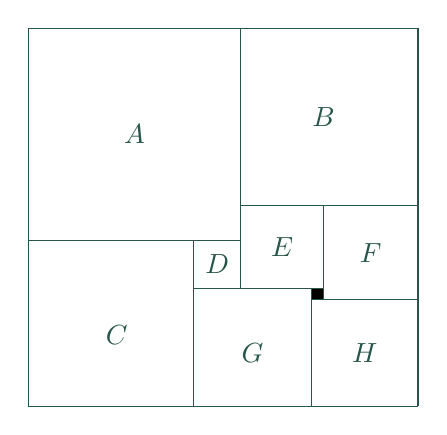
\begin{tikzpicture}[thachthuctoanhoc,scale=0.15]
			\draw[fill=black] (0,0) rectangle (1,1);
			\draw  (0.,-9.)-- (9.,-9.);
			\draw  (9.,-9.)-- (9.,0.);
			\draw (4.5,-4.5) node {$H$};
			\draw (5,4) node {$F$};
			\draw (-2.5,4.5) node {$E$};
			\draw (-5,-4.5) node {$G$};
			\draw (-8,3) node {$D$};
			\draw (1,15.5) node {$B$};
			\draw (-15,14) node {$A$};
			\draw (-16.5,-3) node {$C$};
			\draw  (9.,0.)-- (0.,0.);
			\draw  (0.,0.)-- (0.,-9.);
			\draw  (1.,0.)-- (9.,0.);
			\draw  (9.,0.)-- (9.,8.);
			\draw  (9.,8.)-- (1.,8.);
			\draw  (1.,8.)-- (1.,0.);
			\draw  (-10.,-9.)-- (0.,-9.);
			\draw  (0.,-9.)-- (0.,1.);
			\draw  (0.,1.)-- (-10.,1.);
			\draw  (-10.,1.)-- (-10.,-9.);
			\draw  (-6.,1.)-- (1.,1.);
			\draw  (1.,1.)-- (1.,8.);
			\draw  (1.,8.)-- (-6.,8.);
			\draw  (-6.,8.)-- (-6.,1.);
			\draw  (-10.,1.)-- (-6.,1.);
			\draw  (-6.,1.)-- (-6.,5.);
			\draw  (-6.,5.)-- (-10.,5.);
			\draw  (-10.,5.)-- (-10.,1.);
			\draw  (-6.,8.)-- (9.,8.);
			\draw  (9.,8.)-- (9.,23.);
			\draw  (9.,23.)-- (-6.,23.);
			\draw  (-6.,23.)-- (-6.,8.);
			\draw  (-24.,-9.)-- (-10.,-9.);
			\draw  (-10.,-9.)-- (-10.,5.);
			\draw  (-10.,5.)-- (-24.,5.);
			\draw  (-24.,5.)-- (-24.,-9.);
			\draw  (-24.,5.)-- (-6.,5.);
			\draw  (-6.,5.)-- (-6.,23.);
			\draw  (-6.,23.)-- (-24.,23.);
			\draw  (-24.,23.)-- (-24.,5.);	
		\end{tikzpicture}
		\vspace*{-10pt}
	\end{figure} 
	Gọi $a, b, c, d, e, g, h$ tương ứng là độ dài cạnh của các hình vuông $A, B, C, D, E, G, H$.
	\vskip 0.1cm
	Gọi $x$ là độ dài cạnh của hình vuông $F$.
	\vskip 0.1cm
	Khi đó, do hình vuông màu đen có cạnh bằng $1$, nên
	\begin{align*}
		&e = x - 1; b = e + x = 2x - 1;\\
		&h = x + 1; g = h + 1 = x + 2;\\
		&d = g - (e - 1) = (x + 2) - (x - 2) = 4;\\
		&c = g + d = (x + 2) + 4 = x + 6;\\
		&a = c + d = (x + 6) + 4 = x + 10.
	\end{align*}
	Từ đó, do $a + c = b + x + h$, nên ta có:
	\begin{align*}
		(x + 10) + (x + 6) = (2x - 1) + x + (x + 1).
	\end{align*}
	Suy ra, $2x + 16 = 4x$. Do đó, $x = 8$. Suy ra
	\begin{align*}
		&a = 8 + 10 = 18, b = 2\cdot8 - 1 = 15 \\
		\text{ và } &c = 8 + 6 = 14.
	\end{align*}
	Vì vậy, hình chữ nhật có chiều dài là:
	\begin{align*}
		18 + 15 = 33,
	\end{align*}
	và chiều rộng là: $18 + 14 = 32$.
	\vskip 0.05cm
	\textbf{\color{thachthuctoanhoc}Bình luận và Nhận xét}
	\vskip 0.05cm	
	Tất cả lời giải Tạp chí đã nhận được từ bạn đọc đều là lời giải đúng và hoàn chỉnh.
	\begin{flushright}
		\textbf{\color{thachthuctoanhoc}Hà Thanh}
	\end{flushright}
	{\color{thachthuctoanhoc}{\usefont{T5}{qag}{b}{n} P732.}}
	(Mức $B$) Xét bốn số thực (không nhất thiết đôi một khác nhau), mà mỗi số có trị tuyệt đối không vượt quá $\dfrac{1}{2}$, và tổng của ba số bất kỳ, trong bốn số đó, là một số nguyên. Tìm tất cả các giá trị có thể của tổng bốn số đó.
	\vskip 0.05cm
	\textbf{\color{thachthuctoanhoc}Lời giải} (\textit{phỏng theo cách giải của bạn Ngô Minh Chấn, lớp $9$A$3$, trường TH$\&$THCS Archimedes Đông Anh, Tp. Hà Nội})\textbf{\color{thachthuctoanhoc}.}
	\vskip 0.05cm
	Gọi $a, b, c, d$ là bốn số thực thỏa mãn các điều kiện đã nêu trong đề bài.
	\vskip 0.05cm
	Đặt $x = a \!+\! b \!+\! c$, $y = a \!+\! b \!+\! d$, $z = a \!+\! c \!+\! d$, $t = b + c + d$, và
	$s = a + b + c + d$.
	\vskip 0.05cm
	Khi đó, theo giả thiết của bài ra, ta có:
	\begin{align*}
		|a| \le \frac{1}{2}, |b| \le \frac{1}{2},|c| \le \frac{1}{2},|d| \le \frac{1}{2}; \tag{$1$}
	\end{align*}
	và $x, y, z, t$ là các số nguyên.        \hfill ($2$)
	\vskip 0.05cm
	Xét cặp số $x, y$.
	Do ($2$) nên $x - y$ là một số nguyên; hơn nữa
	\begin{align*}
		\left| {x - y} \right| &= \left| {c - d} \right| \le |c| + \left| {d} \right| \\
		&\le 1 \quad\text{(do ($1$))}. \tag{$3$}
	\end{align*}
	Vì thế, $\left| {x - y} \right| \in \left\{ {0;1} \right\}.$ \hfill ($4$)
	\vskip 0.05cm
	Nếu $|x - y| = 1$  thì theo ($3$), phải có:
	\begin{align*}
		\left| {c - d} \right| = |c| + \left| {d} \right| = 1.
	\end{align*}
	Điều vừa nêu trên tương đương với
	\begin{align*}
	\quad\quad	\begin{cases}
			cd \le 0\\
			|c| = |d| = \dfrac{1}{2} \text{ (do ($1$)).} \quad\quad\quad\quad \text{($5$)} 
		\end{cases}
	\end{align*}
	Suy ra, $c + d = 0$. Do đó, $z = a$ và $t = b$. Vì thế, $a,b \in \mathbb{Z}$  (do ($2$)). Từ đây và ($1$), suy ra $a = b = 0$.
	\vskip 0.05cm
	Vì vậy, $x = c$. Do đó,  $c \in \mathbb{Z}$. Từ đây và ($1$), suy ra $c = 0$, mâu thuẫn với ($5$).
	\vskip 0.05cm
	Mâu thuẫn nhận được ở trên cho thấy
	\begin{align*}
		|x - y| \ne 1.
	\end{align*}
	Do đó, từ ($4$) ta được $x = y$.
	\vskip 0.05cm
	Xét các cặp số $x, z$ và $x, t$, bằng cách hoàn toàn tương tự, ta sẽ được $x = z$ và $x = t$.
	\vskip 0.05cm
	Vì vậy, $x = y = z = t$. Suy ra
	\begin{align*}
		3s = x  + y + z + t = 4x;
	\end{align*}
	do đó, $s = \dfrac{4}{3}x$. \hfill ($6$)
	\vskip 0.05cm
	Tiếp theo, ta có:
	\begin{align*}
		|x| \le |a| + |b| + |c| \le \frac{3}{2} \quad\text{(do ($1$))}; 
	\end{align*}
	mà $|x| \in \mathbb{Z}$  (theo ($2$)), nên  $|x| \in \{0;1\}$. \hfill ($7$)
	\vskip 0.05cm
	Từ ($6$) và ($7$), suy ra $s \in \{-\dfrac{4}{3}; 0; \dfrac{4}{3}\}$.
	\vskip 0.05cm 
	Ngược lại, dễ thấy:
	\vskip 0.05cm
	$\bullet$ $a=b=c=d = -\dfrac{1}{3}$   là bốn số thực thỏa mãn các điều kiện của đề bài, và có tổng bằng $- \dfrac{4}{3}$;
	\vskip 0.05cm  
	$\bullet$  $a=b=c=d = 0$  là bốn số thực thỏa mãn các điều kiện của đề bài, và có tổng bằng $0$;
	\vskip 0.05cm
	$\bullet$ $a=b=c=d = \dfrac{1}{3}$   là bốn số thực thỏa mãn các điều kiện của đề bài, và có tổng bằng $\dfrac{4}{3}$;
	\vskip 0.05cm  
	Vậy, tất cả các giá trị có thể của tổng bốn số thỏa mãn các điều kiện của đề bài là:  $- \dfrac{4}{3}, 0, \dfrac{4}{3}$.
	\vskip 0.05cm  
	\textbf{\color{thachthuctoanhoc}Bình luận và Nhận xét}
	\vskip 0.05cm
	$\pmb{1.}$ Lời giải trên cho thấy, các bộ bốn số thực được liệt kê ở phần cuối của Lời giải là \textit{tất cả} các bộ bốn số thực thỏa mãn các điều kiện của đề bài.
	\vskip 0.05cm
	$\pmb{2.}$ Trong số các lời giải Tạp chí đã nhận được từ bạn đọc, rất tiếc, có hai lời giải sai, do người giải bài hoặc mới chỉ ra điều kiện cần (nhưng không đủ) cho giá trị của tổng bốn số đã vội kết luận đó là các giá trị có thể của tổng đó, hoặc đã chỉ ra sai các bộ bốn số thực thỏa mãn các điều kiện của đề bài. Bên cạnh đó, còn có một lời giải chưa đầy đủ, do người giải bài chưa xét hết các trường hợp có thể xảy~ra.
	\begin{flushright}
		\textbf{\color{thachthuctoanhoc}Hà Thanh}
	\end{flushright}
	{\color{thachthuctoanhoc}{\usefont{T5}{qag}{b}{n} P733.}}
	(Mức $B$)
	Tìm giá trị nhỏ nhất của biểu thức
	\begin{align*}
		S = \left\lfloor {\frac{{b + c}}{a}} \right\rfloor  + \left\lfloor {\frac{{c + a}}{b}} \right\rfloor  + \left\lfloor {\frac{{a + b}}{c}} \right\rfloor ,
	\end{align*}
	trong đó, $a, b, c$ là các biến nguyên dương.
	($\left\lfloor x \right\rfloor $  ký hiệu số nguyên lớn nhất không vượt quá $x$.)
	\vskip 0.05cm
	\textbf{\color{thachthuctoanhoc}Lời giải} (\textit{dựa theo lời giải của các bạn: Ngô Minh Chấn, lớp $9$A$3$, trường TH$\&$THCS Archimedes Đông Anh, Tp. Hà Nội; Lê Nguyễn Hoàng Nhật Đình, lớp $9$C, trường THCS Nguyễn Thái Bình, tỉnh Cà Mau; Trương Anh Dũng, lớp $10$A$1$ chuyên Toán, trường THPT chuyên Vĩnh Phúc, tỉnh Vĩnh Phúc})\textbf{\color{thachthuctoanhoc}.}
	\vskip 0.05cm
	Từ định nghĩa phần nguyên của một số thực dễ thấy, với mọi số thực $x$, ta đều có
	\begin{align*}
		\left\lfloor x \right\rfloor  > x -1.
	\end{align*}
	Vì vậy, với lưu ý $a, b, c$ là các số dương, ta có:
	\begin{align*}
			S &> \frac{{b + c}}{a} + \frac{{c + a}}{b} + \frac{{a + b}}{c} - 3 \\
			&= \left( {\frac{b}{a} + \frac{a}{b}} \right) + \left( {\frac{c}{a} + \frac{a}{c}} \right) + \left( {\frac{c}{b} + \frac{b}{c}} \right) - 3\\
			 &\ge 2\sqrt {\frac{b}{a} \!\cdot\! \frac{a}{b}}  \!+\! 2\sqrt {\frac{c}{a} \!\cdot\! \frac{a}{c}}  \!+\! 2\sqrt {\frac{c}{b} \!\cdot\! \frac{b}{c}}  \!-\! 3 \!=\! 3.
	\end{align*}
	Từ đó, do $S$ là số nguyên, suy ra $S \ge 4$.
	\vskip 0.05cm
	Hơn nữa, dễ thấy, với $a = 3, b = c = 4$, ta có $S = 4$.
	\vskip 0.05cm
	Vì vậy, giá trị nhỏ nhất của $S$ bằng $4$.
	\vskip 0.05cm
	\textbf{\color{thachthuctoanhoc}Bình luận và Nhận xét}
	\vskip 0.05cm
	$\pmb{1.}$ Lời giải trên cho thấy, kết quả của bài ra không thay đổi, khi thay giả thiết ``$a, b, c$ là các biến nguyên dương" bởi giả thiết ``$a, b, c$ là các biến thực dương".
	\vskip 0.05cm
	$\pmb{2.}$ Trong số các lời giải Tạp chí đã nhận được từ bạn đọc, rất tiếc, có một lời giải sai, do người giải bài đã mắc sai sót về kiến thức cơ bản, khi khẳng định ``$\left\lfloor x \right\rfloor  \ge x$  với mọi số thực $x$".
	\begin{flushright}
		\textbf{\color{thachthuctoanhoc}Lưu Thị Thanh Hà}
	\end{flushright}
	{\color{thachthuctoanhoc}{\usefont{T5}{qag}{b}{n} P734.}}
	(Mức $B$) Cho hình vuông $ABCD$. Gọi $E$ là trung điểm của $AD$; $H$ là hình chiếu vuông góc của $B$ trên $CE$. Trên đường chéo $AC$, lấy điểm $M$ sao cho $AM = \dfrac{3}{8}AC$. Chứng minh rằng, $ME$ song song với $DH$.
	\vskip 0.05cm
	\textbf{\color{thachthuctoanhoc}Lời giải} (\textit{dựa theo lời giải của bạn Nguyễn Nguyên Chinh, lớp $9$D, trường THCS Nguyễn Chí Thanh, tỉnh Phú Yên})\textbf{\color{thachthuctoanhoc}.}
	\begin{figure}[H]
		\vspace*{-5pt}
		\centering
		\captionsetup{labelformat= empty, justification=centering}
		\definecolor{qqwuqq}{rgb}{0.,0.39215686274509803,0.}
		\definecolor{uuuuuu}{rgb}{0.26666666666666666,0.26666666666666666,0.26666666666666666}
		\definecolor{qqqqff}{rgb}{0.,0.,1.}
		\begin{tikzpicture}[thachthuctoanhoc,scale=0.45]
			\draw [shift={(10.,5.)},pattern color=qqwuqq,fill=qqwuqq,fill opacity=0.10000000149011612] (0,0) -- (-116.56505117707799:0.8153190950798923) arc (-116.56505117707799:-90.:0.8153190950798923) -- cycle;
			\draw [shift={(10.,-4.)},pattern color=qqwuqq,fill=qqwuqq,fill opacity=0.10000000149011612] (0,0) -- (153.43494882292202:0.8153190950798923) arc (153.43494882292202:180.:0.8153190950798923) -- cycle;
			\draw[pattern color=qqwuqq,fill=qqwuqq,fill opacity=0.10000000149011612] (6.743768714703979,-2.3718843573519894) -- (6.915653072055969,-2.028115642648011) -- (6.57188435735199,-1.8562312852960212) -- (6.4,-2.2) -- cycle; 
			\draw[pattern color=qqwuqq,fill=qqwuqq,fill opacity=0.10000000149011612] (1.3843451073079143,-4.) -- (1.3843451073079143,-3.6156548926920857) -- (1.,-3.6156548926920857) -- (1.,-4.) -- cycle; 
			\draw  (1.,5.)-- (10.,5.);
			\draw  (1.,-4.)-- (10.,-4.);
			\draw  (10.,-4.)-- (10.,5.);
			\draw  (1.,5.)-- (10.,-4.);
			\draw [color=qqqqff] (1.,0.5)-- (4.375,1.625);
			\draw  (1.,0.5)-- (10.,-4.);
			\draw [color=qqqqff] (6.4,-2.2)-- (1.,-4.);
			\draw  (6.4,-2.2)-- (10.,5.);
			\draw  (1.,-7.)-- (1.,-4.);
			\draw [color=qqqqff] (1.,-7.)-- (10.,-4.);
			\draw (-0.44481130622791615,6.007702325581402) node[anchor=north west] {$A$};
			\draw (10.011222021831985,6.134879628750732) node[anchor=north west] {$B$};
			\draw (10.038399325001315,-3.477176480514691) node[anchor=north west] {$C$};
			\draw (-0.2002155777039485,-3.341289964668042) node[anchor=north west] {$D$};
			\draw (-0.2002155777039485,1.1157877551020416) node[anchor=north west] {$E$};
			\draw (5.934626546432524,-2.20639567157095424) node[anchor=north west] {$H$};
			\draw (4.30398835627274,2.55618482307652) node[anchor=north west] {$M$};
			\draw (0.44481130622791615,-6.92807467172924) node[anchor=north west] {$N$};
			\draw  (1.,0.5)-- (1.,5.);
			\draw  (0.8777021357380159,2.7024397194536727) -- (1.1222978642619836,2.7024397194536727);
			\draw  (0.8777021357380159,2.797560280546327) -- (1.1222978642619836,2.797560280546327);
			\draw  (1.,0.5)-- (1.,-4.);
			\draw  (1.1222978642619836,-1.7024397194536725) -- (0.8777021357380159,-1.7024397194536725);
			\draw  (1.1222978642619836,-1.7975602805463267) -- (0.8777021357380159,-1.7975602805463267);
				\draw [fill=qqqqff] (1.,5.) circle (1.5pt);
				\draw [fill=qqqqff] (10.,5.) circle (1.5pt);
				\draw [fill=qqqqff] (10.,-4.) circle (1.5pt);
				\draw [fill=qqqqff] (1.,-4.) circle (1.5pt);
				\draw [fill=uuuuuu] (1.,0.5) circle (1.5pt);
				\draw [fill=qqqqff] (4.375,1.625) circle (1.5pt);
				\draw [fill=uuuuuu] (6.4,-2.2) circle (1.5pt);
				\draw [fill=uuuuuu] (1.,-7.) circle (1.5pt);
		\end{tikzpicture}
		\vspace*{-10pt}
	\end{figure}
	Qua $C$, kẻ đường thẳng song song với $ME$, cắt đường thẳng $AD$ tại $N$.
	\vskip 0.05cm
	Khi đó, theo định lý Thales, ta có:
	\begin{align*}
		\frac{{AN}}{{AE}} = \frac{{AC}}{{AM}} = \frac{8}{3} \quad\text{(theo giả thiết).}
	\end{align*}
	Từ đó, với lưu ý $E$ là trung điểm của $AD$ (giả thiết), suy ra
	\begin{align*}
		\frac{{DN}}{{DE}} = \frac{{DN}}{{AE}} = \frac{{AN}}{{AE}} - \frac{{AD}}{{AE}} = \frac{8}{3} - 2 = \frac{2}{3}.
	\end{align*}
	Do đó
	\begin{align*}
		\frac{{NE}}{{ND}} &= \frac{{ND + DE}}{{ND}} = 1 + \frac{{DE}}{{ND}} \\
		&= 1 + \frac{3}{2} = \frac{5}{2}. \tag{$1$}
	\end{align*}
	Đặt $AD = a$. Từ giả thiết của bài ra, ta có $CD = a$ và
	\begin{align*}
		AE = \frac{{AD}}{2} = \frac{a}{2}.
	\end{align*}
	Vì vậy, áp dụng định lý Pithagoras cho tam giác vuông $CDE$, ta được:
	\begin{align*}
		C{E^2} &= C{D^2} + D{E^2} \\
		&= {a^2} + {\left( {\frac{a}{2}} \right)^2} = \frac{5}{4}{a^2}. \tag{$2$}
	\end{align*}
	Tiếp theo, do
	\begin{align*}
		\angle CBH = {90^{\rm{o}}} - \angle BCH = \angle DCE,
	\end{align*}
	nên tam giác vuông $BHC$ đồng dạng với tam giác vuông $CDE$. Do đó
	\begin{align*}
		\frac{{CH}}{{CB}} = \frac{{ED}}{{EC}};
	\end{align*}
	suy ra
	\begin{align*}
			\frac{{CH}}{{CE}} = \frac{{ED \cdot CB}}{{C{E^2}}} = \frac{{\dfrac{a}{2} \cdot a}}{{\dfrac{5}{4}{a^2}}}\quad\left( {{\rm{theo}}(2)} \right)\\
			 = \frac{2}{5} = \frac{{ND}}{{NE}}\quad\left( {{\rm{theo}}(1)} \right).
	\end{align*}
	Do đó, $DH \parallel NC$ (theo định lý Thales); mà $NC \parallel ME$, nên $DH \parallel ME$.
	\vskip 0.05cm
	Ta có điều phải chứng minh theo yêu cầu đề bài. 
	\vskip 0.05cm
	\textbf{\color{thachthuctoanhoc}Bình luận và Nhận xét}
	\vskip 0.05cm
	Trong số các lời giải Tạp chí đã nhận được từ bạn đọc, có một lời giải bằng phương pháp tọa độ. Rất tiếc, lời giải này được diễn đạt rất sai bằng ngôn ngữ Toán học; và vì thế, không thể coi là lời giải đúng.
	\begin{flushright}
		\textbf{\color{thachthuctoanhoc}Hạ Vũ Anh}
	\end{flushright}
	{\color{thachthuctoanhoc}{\usefont{T5}{qag}{b}{n} P735.}}
	(Mức $B$) Tìm tất cả các số nguyên dương $n$, để $n! + n$ là một lũy thừa với số mũ nguyên dương của một số nguyên tố.
	\vskip 0.05cm
	\textbf{\color{thachthuctoanhoc}Lời giải} (\textit{dựa theo đa số lời giải Tạp chí đã nhận được từ bạn đọc})\textbf{\color{thachthuctoanhoc}.}
	\vskip 0.05cm
	$\bullet$ Giả sử $n$ là số nguyên dương thỏa mãn yêu cầu đề bài.
	\vskip 0.05cm
	Khi đó, tồn tại số nguyên tố $p$ và số nguyên dương $\alpha$, sao cho
	\begin{align*}
		n! + n = {p^\alpha },
	\end{align*}
	hay  
	\begin{align*}
		n\left( {\left( {n - 1} \right)! + 1} \right) = {p^\alpha }. \tag{$1$}
	\end{align*}
	Do $\left( {n - 1} \right)! + 1 > 1$  nên từ ($1$) suy ra, tồn tại số tự nhiên $\beta < \alpha$, sao cho $n = p^{\beta}$  và
	\begin{align*}
		\left( {n - 1} \right)! + 1 = {p^{\alpha  - \beta }}. \tag{$2$}
	\end{align*}
	Vì  $\beta \in  \mathbb{N}, \alpha \in \mathbb{N^*}$   và $\beta < \alpha$, nên  $\alpha - \beta$ là một số nguyên dương. Do đó, từ ($2$) suy ra
	\begin{align*}
		\left( {n - 1} \right)! + 1 \equiv 0\left( {\bmod p} \right). \tag{$3$}
	\end{align*}
	Từ ($2$) và ($3$) suy ra $\beta \in \{0;1\}$, vì nếu ngược lại, $\beta \ge 2$,  thì
	\begin{align*}
		n - 1 \ge {p^2} - 1 > p \text{ (do $n = p^{\beta}$  và $p \ge 2$)};
	\end{align*}
	dẫn tới $\left( {n - 1} \right)! \,\,\vdots\,\, p,$  và do đó,  $1 \,\,\vdots\,\, p$ (theo ($3$)), là điều vô lý.
	\vskip 0.05cm
	Với $\beta= 0$, ta có $n = p^0 = 1$. \hfill ($4$)
	\vskip 0.05cm
	Với $\beta = 1$, ta có $n = p$; do đó
	\begin{align*}
		\left( {p - 1} \right)! + 1 = {p^{\alpha  - 1}}	\quad\text{(theo ($2$))}. \tag{$5$}
	\end{align*}                                                      
	Xét $p > 5$. Khi đó
	\begin{align*}
		\left( {p - 1} \right)! > \left( {p - 1} \right)\left( {p - 2} \right) > p.
	\end{align*}
	Vì thế, từ ($5$) suy ra $\alpha -1\ge 2$, hay $\alpha \ge 3$. Do vậy, từ ($5$) ta có:
	\begin{align*}
		&\left( {p - 1} \right)! = {p^{\alpha  - 1}} - 1 \\
		=\, &\left( {p - 1} \right)\left( {{p^{\alpha  - 2}} + {p^{\alpha  - 3}} +  \cdots  + p + 1} \right).
	\end{align*}
	Suy ra
	\begin{align*}
		\left( {p \!-\! 2} \right)! \!=\! {p^{\alpha  \!-\! 2}} \!+\! {p^{\alpha  \!-\! 3}} \!+\!  \cdots  \!+\! p \!+\! 1. \tag{$6$}
	\end{align*}
	Tiếp theo, do $p$ là số nguyên tố lớn hơn $5$ nên $p - 1$ là một hợp số lớn hơn $4$. Vì thế, tồn tại các số nguyên dương $a, b$, với $1 < a \le b$, sao cho $p - 1 = ab$.
	\vskip 0.05cm
	-- Nếu $a = b$ thì
	\begin{align*}
		4 < p - 1 = {a^2}. \tag{$7$}
	\end{align*}
	Do đó, $a > 2$; suy ra $p - 1 > 2a$. Vì thế, $p - 2 > 2a - 1$; mà $p - 2$ là số nguyên, nên $p - 2 \ge 2a$. Vì vậy
	\begin{align*}
	\left( {p - 2} \right)! &= 1 \cdot 2 \cdot  \cdots  \cdot a \cdot  \cdots  \cdot 2a \cdot  \cdots  \cdot \left( {p - 2} \right) \\
	&\equiv 0\left(\!\! {\bmod p - 1} \right)	\,\,\,\text{(do ($7$))}.
	\end{align*}
	-- Nếu $a < b$ thì do $a, b < p - 2$ nên
	\begin{align*}
		\left( {p - 2} \right)! &= 1 \cdot 2 \cdot  \cdots  \cdot a \cdot  \cdots  \cdot b \cdot  \cdots  \cdot \left( {p - 2} \right) \\
		&\equiv 0\left(\!\! {\bmod p - 1} \right) \,\,\,\text{(do $p - 1 = ab$).}
	\end{align*}
	Vì vậy, ta có
	\begin{align*}
		\left( {p - 2} \right)! \equiv 0\left( {\bmod p - 1} \right). \tag{$8$}
	\end{align*}
	Do $p \equiv 1\left( {\bmod p - 1} \right)$  nên từ ($6$) suy ra
	\begin{align*}
		\left( {p - 2} \right)! \equiv \alpha  - 1\left( {\bmod p - 1} \right). \tag{$9$}
	\end{align*}
	Từ ($8$) và ($9$), ta được:
	\begin{align*}
		\alpha  - 1 \equiv 0\left( {\bmod p - 1} \right);
	\end{align*}
	mà $\alpha - 1$ là số nguyên dương, nên $\alpha - 1 \ge p - 1$, hay $\alpha \ge p$. Vì thế, theo ($5$), ta có
	\begin{align*}
		\left( {p - 1} \right)! + 1 \ge {p^{p - 1}},
	\end{align*}
	là điều vô lý.
	\vskip 0.05cm
	Điều vô lý vừa nhận được ở trên cho thấy, $p \le 5$; mà $p$ là số nguyên tố, nên \linebreak$p \in \{2; 3; 5\}$. \hfill      ($10$)
	\vskip 0.05cm
	Do $n = p$ nên từ ($4$) và ($10$), ta được: \linebreak$n \in \{1; 2; 3; 5\}$. \hfill ($11$)
	\vskip 0.05cm
	$\bullet$ Ngược lại, với $n$ thỏa mãn ($11$), ta có
	\begin{align*}
		n! + n \in S = \{2; 4; 9; 125\}.
	\end{align*}
	Dễ thấy, mỗi số thuộc $S$ đều là một lũy thừa với số mũ nguyên dương của một số nguyên tố.
	\vskip 0.05cm
	$\bullet$ Vậy, tất cả các số nguyên dương cần tìm theo yêu cầu đề bài là: $1, 2, 3$ và $5$.
	\vskip 0.05cm 
	\textbf{\color{thachthuctoanhoc}Bình luận và Nhận xét}
	\vskip 0.05cm
	$\pmb{1.}$ Dễ thấy, trong Lời giải trên ẩn chứa chứng minh của kết quả sau:
	\vskip 0.05cm
	``\textit{Nếu $n$ là một hợp số lớn hơn $4$ thì}  
	\begin{align*}
		\left( {n - 1} \right)! \equiv 0\left( {\bmod n} \right)."
	\end{align*}
	$\pmb{2.}$ Trong số các lời giải Tạp chí nhận được từ bạn đọc, rất tiếc, có một lời giải sai (do người giải bài mắc một số sai sót trong các lập luận) và một lời giải chưa đầy đủ (do người giải bài chưa xét trường hợp $n = 1$).
	\begin{flushright}
		\textbf{\color{thachthuctoanhoc}Lưu Thị Thanh Hà}
	\end{flushright}
	{\color{thachthuctoanhoc}{\usefont{T5}{qag}{b}{n} P736.}}
	(Mức $B$) Bạn An có $8$ quả cân có tổng trọng lượng bằng $16$ kg, và trọng lượng mỗi quả, tính theo đơn vị kg, là một số nguyên dương không vượt quá $8$. Chứng minh rằng, có thể chia $8$ quả cân này thành hai nhóm, sao cho các tổng trọng lượng của các quả cân cùng nhóm bằng nhau.
	\vskip 0.05cm
	\textbf{\color{thachthuctoanhoc}Lời giải} (\textit{dựa theo cách giải của bạn Phạm Đức Minh, lớp $10$ Toán $2$, trường THPT chuyên Lê Hồng Phong, tỉnh Nam Định})\textbf{\color{thachthuctoanhoc}.}
	\vskip 0.05cm
	Dễ thấy, nếu cả $8$ quả cân có trọng lượng như nhau thì điều phải chứng minh theo yêu cầu đề bài là hiển nhiên.
	\vskip 0.05cm
	Xét trường hợp trong $8$ quả cân, tồn tại hai quả cân có trọng lượng khác nhau. Gọi $m_1, m_2$  ($m_1 \ne m_2$) là trọng lượng của hai quả cân này; và gọi $m_3, m_4, m_5,m_6,m_7,m_8$  là trọng lượng của sáu quả cân còn lại.
	\vskip 0.05cm
	Hiển nhiên, kết luận của bài ra tương đương với khẳng định ``tồn tại một nhóm gồm tối đa $7$ quả cân và tổng trọng lượng của các quả cân thuộc nhóm bằng $8$".
	\vskip 0.05cm
	Vì vậy, để chứng minh kết luận của bài ra, ta sẽ chỉ ra một nhóm gồm tối đa $7$ quả cân và tổng trọng lượng của các quả cân thuộc nhóm bằng $8$. Để tránh dài dòng trong diễn đạt, ta gọi nhóm quả cân có tính chất vừa nêu là nhóm ``\textit{tốt}".
	\vskip 0.05cm
	Đặt
	\begin{align*}
		&{S_1} = {m_1},{S_2} = {m_2},{S_3} = {m_1} + {m_2},\\
		&{S_4} = {m_1} \!+\! {m_2} \!+\! {m_3},
		{S_5} = {m_1} \!+\! {m_2} \!+\! {m_3} \!+\! {m_4},\\
		&{S_6} = {m_1} + {m_2} + {m_3} + {m_4} + {m_5},\\
		&{S_7} = {m_1} + {m_2} + {m_3} + {m_4} + {m_5} + {m_6},\\
		&{S_8} = {m_1} + {m_2} + {m_3} + {m_4} + {m_5} + {m_6} + {m_7}.
	\end{align*}
	Từ giả thiết của đề bài suy ra $S_1,S_2$  là các số nguyên dương không vượt quá $8$, và \linebreak$S_i, i = \overline{3,8}$,  là các số nguyên dương không vượt quá $15$.
	\vskip 0.05cm
	Xảy ra hai trường hợp sau:
	\vskip 0.05cm
	$\bullet$ \textit{Trường hợp} $1$: Tồn tại $i \in \{1; 2; \ldots; 8\}$ sao cho ${S_i} \equiv 0\left( {\bmod 8} \right).$
	\vskip 0.05cm 
	Khi đó, do $S_i \in \mathbb{N^*}$  và $1 \le S_i \le 15$,  nên $S_i = 8$.  Vì thế, nhóm gồm các quả cân có trọng lượng là các số hạng của tổng $S_i$  là một nhóm tốt.
	\vskip 0.05cm
	$\bullet$ \textit{Trường hợp} $2$: Với mọi $i \in \{1; 2; \ldots; 8\}$,  ${S_i}\not  \equiv 0\left( {\bmod 8} \right).$
	\vskip 0.05cm
	Trong trường hợp này, do phép chia cho $8$ chỉ có $7$ số dư khác $0$, nên theo nguyên lý Dirichlet, tồn tại các chỉ số $p$, $q$, với $1 \le p < q \le 8$, sao cho
	\begin{align*}
		{S_p} \equiv {S_q}\left( {\bmod 8} \right). \tag{$1$}
	\end{align*}
	Do ${S_1},{S_2} \in \left\{ {1;2; \ldots ;8} \right\}$ (giả thiết) và  ${S_1},{S_2}\not  \equiv 0\left( {\bmod 8} \right),$ nên ${S_1},{S_2} \in \left\{ {1;2; \ldots ;7} \right\}.$  Mà $S_1 \ne S_2$  (do  $m_1 \ne m_2$), nên ${S_1}\not  \equiv {S_2}\left( {\bmod 8} \right).$  Vì thế, không thể có đồng thời $p = 1$ và $q = 2$. \hfill    ($2$)
	\vskip 0.05cm
	Đặt  $T = S_q - S_p$.
	\vskip 0.05cm
	Do ($2$) và do $1 \le {S_p},{S_q} \le 15$  nên \linebreak$T \in \mathbb{N^*}, 1 \le T \le 14$,    và
	\begin{align*}
	\!T\!=\!	\begin{cases}
			m_2 + m_3 + \cdots + m_{q-1} \text{ nếu } p=1 \\
			m_1 + m_3 + \cdots + m_{q-1} \text{ nếu } p=2 \\
			m_p \!+\! m_{p\!+\!1} \!+\! \cdots \!+\! m_{q-1} \text{ nếu } 3 \!\le\! p \!\le\! 7.\\
		\end{cases}
	\end{align*}
	Do ($1$) nên  $T \equiv 0\left( {\bmod 8} \right);$ mà $1 \le T \le 14$ (theo trên), nên $T = 8$. Vì thế, nhóm gồm các quả cân có trọng lượng là các số hạng của tổng $T$ là một nhóm tốt.
	\vskip 0.05cm
	Kết quả xét hai trường hợp trên đây cho ta điều phải chứng minh theo yêu cầu đề bài.
	\vskip 0.05cm
	\textbf{\color{thachthuctoanhoc}Bình luận và Nhận xét}
	\vskip 0.05cm
	$\pmb{1.}$ Bài đã ra có thể được phát biểu dưới dạng tương đương sau:
	\vskip 0.05cm
	``\textit{Cho tám số nguyên dương (không nhất thiết đôi một khác nhau) không vượt quá $8$ và có tổng bằng $16$. Chứng minh rằng, tồn tại một nhóm gồm tối đa bảy số, trong tám số đó, mà tổng các số thuộc nhóm bằng $8$.}"
	\vskip 0.05cm
	Với các bài toán ``kiểu" trên, ý tưởng ``từ các số đã cho, thiết lập các tổng ``con", rồi xét các tổng đó theo một modulo thích hợp", là một ý tưởng tự nhiên và thông dụng.
	\vskip 0.05cm
	$\pmb{2.}$ Tất cả lời giải Tạp chí đã nhận được từ bạn đọc đều có ý tưởng giải là ý tưởng vừa nêu trên.
	\vskip 0.05cm
	\hfill	\textbf{\color{thachthuctoanhoc}Nguyễn Khắc Minh}
	\vskip 0.05cm
	{\color{thachthuctoanhoc}{\usefont{T5}{qag}{b}{n} P737.}}
	(Mức $A$) Xét các số thực dương $a, b, c$, thỏa mãn $a^2 + b^2 + c^2 =1$.  Tìm giá trị nhỏ nhất của biểu thức
	\begin{align*}
		S = 2\left( {{a^3} + {b^3} + {c^3}} \right) - \left( {a + b + c} \right).
	\end{align*}
	\textbf{\color{thachthuctoanhoc}Lời giải} (\textit{của người chấm bài})\textbf{\color{thachthuctoanhoc}.}
	\vskip 0.05cm
	Do $a, b, c > 0$ và $a^2 + b^2 + c^2 = 1$,  nên theo bất đẳng thức Cauchy -- Schwarz, ta có:
	\begin{align*}
		&{\left( {a + b + c} \right)^2} \\
		\le &\left( {1 + 1 + 1} \right)\left( {{a^2} + {b^2} + {c^2}} \right) = 3; \tag{$1$}\\
		&\left( {{a^3} + {b^3} + {c^3}} \right)\left( {a + b + c} \right) \\
		\ge &{\left( {{a^2} + {b^2} + {c^2}} \right)^2} = 1. \tag{$2$}
	\end{align*}
	Do $a, b, c > 0$ nên từ ($1$) suy ra
	\begin{align*}
		a + b + c \le \sqrt 3 . \tag{$3$}
	\end{align*}
	Lại do $a, b, c > 0$ nên từ ($2$) và ($3$), suy ra
	\begin{align*}
		{a^3} + {b^3} + {c^3} \ge \frac{1}{{a + b + c}} \ge \frac{1}{{\sqrt 3 }}. \tag{$4$}
	\end{align*}
	Từ ($3$) và ($4$), ta được:
	\begin{align*}
		S \ge 2 \cdot \frac{1}{{\sqrt 3 }} - \sqrt 3  =  - \frac{1}{{\sqrt 3 }}.
	\end{align*}
	Hơn nữa, dễ thấy, với $a = b = c = \frac{1}{{\sqrt 3 }},$  ta có $a^2 + b^2 + c^2 = 1$  và $S = - \dfrac{1}{\sqrt{3}}$.
	\vskip 0.05cm 
	Vì vậy, giá trị nhỏ nhất của $S$ bằng  $- \dfrac{1}{\sqrt{3}}$.
	\vskip 0.05cm 
	\textbf{\color{thachthuctoanhoc}Bình luận và Nhận xét}
	\vskip 0.05cm
	$\pmb{1.}$ Bài đã ra là một bài toán cơ bản, một ví dụ đơn giản minh họa việc sử dụng bất đẳng thức Cauchy -- Schwarz trong chứng minh bất đẳng thức.
	\vskip 0.05cm
	$\pmb{2.}$ Dù đã được nhắc rất nhiều lần trên Tạp chí, vẫn có quá nửa số lời giải, mà Tạp chí đã nhận được từ bạn đọc, mắc lỗi kiến thức cơ bản. Đó là, khẳng định giá trị nhỏ nhất của $S$ bằng  $-\dfrac{1}{\sqrt{3}}$, \textit{ngay sau khi mới chỉ chứng minh được} $S \ge - \dfrac{1}{\sqrt{3}}$.  
	\vskip 0.05cm
	\hfill	\textbf{\color{thachthuctoanhoc}Võ Quốc Bá Cẩn}
	\vskip 0.1cm
	{\color{thachthuctoanhoc}{\usefont{T5}{qag}{b}{n} P738.}}
	(Mức $A$) Cho tam giác $ABC$ ngoại tiếp đường tròn $(I)$. Gọi $J$ là tâm đường tròn bàng tiếp góc $A$ của tam giác đó. Trên cạnh $BC$, lấy điểm $D$ tùy ý, sao cho ba điểm $A, I, D$ không thẳng hàng. Đường thẳng $AD$ cắt các đường thẳng $IB$, $IC$, tương ứng, tại $E$, $F$. Gọi $H$ là trực tâm của tam giác $IEF$, và gọi $K$ là trung điểm của $AD$. Chứng minh ba điểm $K$, $H$, $J$ thẳng hàng.
	\vskip 0.05cm
	\textbf{\color{thachthuctoanhoc}Lời giải} (\textit{dựa theo Đáp án của BBT Tạp chí})\textbf{\color{thachthuctoanhoc}.}
	\vskip 0.05cm
	Gọi $G$ là giao điểm của $AJ$ và $BC$; và gọi $M$, $N$ tương ứng là giao điểm của $AD$ với các đường thẳng $BJ$, $CJ$.
	\begin{figure}[H]
		\vspace*{-20pt}
		\centering
		\captionsetup{labelformat= empty, justification=centering}
		\includegraphics[width= 0.98\linewidth]{P738}
%		\caption{\small\textit{\color{}}}
		\vspace*{-20pt}
	\end{figure}
	Do $I$ là tâm đường tròn nội tiếp và $J$  là tâm đường tròn bàng tiếp góc $A$ của tam giác $ABC$, nên $BI$, $BJ$ tương ứng là phân giác trong, phân giác ngoài của góc $ABG$. Do đó, $IB \bot BJ$, và  $\left( {AGIJ} \right) =  - 1.$ Từ đây, do phép chiếu xuyên tâm bảo toàn tỷ số kép, nên
	\begin{align*}
		(ADEM) = B(ADEM) = B(AGIJ)= -1.
	\end{align*}
	Vì thế, do $K$ là trung điểm của $AD$, nên theo hệ thức Newton, ta có:
	\begin{align*}
		K{D^2} = \overline {KE}  \cdot \overline {KM} . \tag{$1$}
	\end{align*}
	Bằng cách tương tự, ta cũng chứng minh được
	\begin{align*}
		K{D^2} = \overline {KF}  \cdot \overline {KN} . \tag{$2$}
	\end{align*}
	Từ ($1$) và ($2$), suy ra
	\begin{align*}
		\overline {KE}  \cdot \overline {KM}  = \overline {KF}  \cdot \overline {KN} ;
	\end{align*}
	do đó, $\dfrac{{\overline {KE} }}{{\overline {KN} }} = \dfrac{{\overline {KF} }}{{\overline {KM} }}.$ \hfill ($3$)
	\vskip 0.05cm
	Đặt $\dfrac{{\overline {KE} }}{{\overline {KN} }} = k$;  và ký hiệu $f$ là phép vị tự tâm $K$, tỷ số $k$.
	\vskip 0.05cm
	Từ ($3$) suy ra, $f$ biến điểm $N$ thành điểm $E$, và biến điểm $M$ thành điểm $F$. \hfill ($4$)
	\vskip 0.05cm
	Tiếp theo, do $H$ là trực tâm tam giác $IEF$ (giả thiết) nên $FH \bot IE$, hay $FH \bot IB$ (do $I$, $E$, $B$ thẳng hàng). Mà $BJ \bot IB$ (chứng minh trên), hay $MJ \bot IB$ (do $M, B, J$ thẳng hàng), nên $FH \parallel MJ$.   \hfill     ($5$)
	\vskip 0.05cm
	Bằng cách hoàn toàn tương tự, ta cũng chứng minh được $EH \parallel NJ$.  \hfill   ($6$)
	\vskip 0.05cm
	Từ ($4$), ($5$) và ($6$) suy ra, $f$ biến đường thẳng $MJ$ thành đường thẳng $FH$, và biến đường thẳng $NJ$ thành đường thẳng $EH$. Do đó, $f$ biến điểm $J$ thành điểm $H$. Mà $K$ là tâm của $f$, nên $K, J, H$ thẳng hàng. Ta có điều phải chứng minh theo yêu cầu đề bài.
	\vskip 0.05cm
	\textbf{\color{thachthuctoanhoc}Bình luận và Nhận xét}
	\vskip 0.05cm
	$\pmb{1.}$ Lời giải trên cho thấy, kết luận của bài ra vẫn đúng, khi thay giả thiết ``$D$ thuộc cạnh $BC$, sao cho $A$, $I$, $D$ không thẳng hàng" bởi giả thiết ``$D$ thuộc đường thẳng $BC$, sao cho $A$, $I$, $D$ không thẳng hàng".
	\vskip 0.05cm
	$\pmb{2.}$ Tất cả các lời giải Tạp chí nhận được từ bạn đọc là lời giải đúng.
	\begin{flushright}
		\textbf{\color{thachthuctoanhoc}Hạ Vũ Anh}
	\end{flushright}
	{\color{thachthuctoanhoc}{\usefont{T5}{qag}{b}{n} P739.}}
	(Mức $A$) Cho dãy số $\left(a_n\right)$  xác định bởi
	\begin{align*}
		{a_n} = \left\lfloor {\frac{n}{{\sqrt 2 }}} \right\rfloor  + \left\lfloor {\frac{n}{{\sqrt 3 }}} \right\rfloor , \text{ với mọi } n \in \mathbb{N^*}.
	\end{align*}
	Chứng minh rằng, trong dãy $\left(a_n\right)$  có vô hạn số chẵn và vô hạn số lẻ.
	\vskip 0.1cm
	($\left\lfloor x \right\rfloor $  ký hiệu số nguyên lớn nhất không vượt quá $x$.)
	\vskip 0.05cm
	\textbf{\color{thachthuctoanhoc}Lời giải} (\textit{dựa trên ý tưởng của bạn Huỳnh Nguyễn Khánh Duy, lớp $12$ Toán, trường THPT chuyên Tiền Giang, tỉnh Tiền Giang})\textbf{\color{thachthuctoanhoc}.}
	\vskip 0.05cm
	Ta có Nhận xét sau:
	\vskip 0.05cm
	\textit{Nhận xét.} Với mọi  $x,y \in \mathbb{R}$, do 
	\begin{align*}
		x - 1 < \left\lfloor x \right\rfloor  \le x  \text{ và } y - 1 < \left\lfloor y \right\rfloor  \le y,
	\end{align*}
	nên
	\begin{align*}
		x - y - 1 < \left\lfloor x \right\rfloor  - \left\lfloor y \right\rfloor  < x - y + 1.
	\end{align*}
	Với mỗi $n \in \mathbb{N^*}$,  đặt
	\begin{align*}
		&{u_n} = \left\lfloor {\frac{{n + 1}}{{\sqrt 2 }}} \right\rfloor  - \left\lfloor {\frac{n}{{\sqrt 2 }}} \right\rfloor \\
		\text{ và } &{v_n} = \left\lfloor {\frac{{n + 1}}{{\sqrt 3 }}} \right\rfloor  - \left\lfloor {\frac{n}{{\sqrt 3 }}} \right\rfloor .
	\end{align*}  
	Theo Nhận xét, với mọi $n \in \mathbb{N^*}$, ta có:
	\begin{align*}
		&- 1 + \frac{1}{{\sqrt 2 }} = \frac{{n + 1}}{{\sqrt 2 }} - \frac{n}{{\sqrt 2 }} - 1 \\
		<\, &{u_n} < \frac{{n + 1}}{{\sqrt 2 }} - \frac{n}{{\sqrt 2 }} + 1 = 1 + \frac{1}{{\sqrt 2 }};
	\end{align*}
	mà $u_n \in \mathbb{Z}$  nên
	\begin{align*}
		u_n \in \{0;1\}  \text{ với mọi } n \in \mathbb{N^*}. \tag{$1$}
	\end{align*}
	Bằng cách hoàn toàn tương tự, ta cũng chứng minh được: 
	\begin{align*}
		v_n \in \{0;1\},  \text{ với mọi } n \in \mathbb{N^*}. \tag{$2$}
	\end{align*}
	Xét số nguyên dương $k$ tùy ý.
	\vskip 0.05cm
	Theo Nhận xét, ta có:
	\begin{align*}
		\sum\limits_{i = k}^{k + 100} {{u_i}}  &= \sum\limits_{i = k}^{k + 100} {\left( {\left\lfloor {\frac{{i + 1}}{{\sqrt 2 }}} \right\rfloor  - \left\lfloor {\frac{i}{{\sqrt 2 }}} \right\rfloor } \right)}  \\
		&= \left\lfloor {\frac{{k + 101}}{{\sqrt 2 }}} \right\rfloor  - \left\lfloor {\frac{k}{{\sqrt 2 }}} \right\rfloor  \\
		&> \frac{{k + 101}}{{\sqrt 2 }} - \frac{k}{{\sqrt 2 }} - 1 = \frac{{101}}{{\sqrt 2 }} - 1 \\
		&> 70, \tag{$3$}\\
		\sum\limits_{i = k}^{k + 100} {{v_i}}  &= \sum\limits_{i = k}^{k + 100} {\left( {\left\lfloor {\frac{{i + 1}}{{\sqrt 3 }}} \right\rfloor  - \left\lfloor {\frac{i}{{\sqrt 3 }}} \right\rfloor } \right)}  \\
		&= \left\lfloor {\frac{{k + 101}}{{\sqrt 3 }}} \right\rfloor  - \left\lfloor {\frac{k}{{\sqrt 3 }}} \right\rfloor \\
		& < \frac{{k + 101}}{{\sqrt 3 }} - \frac{k}{{\sqrt 3 }} + 1 = \frac{{101}}{{\sqrt 3 }} + 1\\
		& < 60. \tag{$4$}
	\end{align*}
	\vskip 0.1cm
	\columnbreak
	Từ ($1$) và ($3$) suy ra, trong $101$ số ${u_k},{u_{k \!+\! 1}},\! \ldots \!,{u_{k \!+\! 100}}$ có ít nhất $71$ số bằng $1$.
	\vskip 0.05cm
	Từ ($2$) và ($4$) suy ra, trong $101$ số ${v_k},{v_{k + 1}}, \ldots ,{v_{k + 100}}$  có tối đa $59$ số bằng $1$.
	\vskip 0.05cm
	Vì vậy, tồn tại $m \in \{k; k + 1; \ldots; k + 100\}$ sao cho $u_m = 1$  và $v_m = 0$.
	\vskip 0.05cm 
	Ta có:
	\begin{align*}
		&{a_{m + 1}} - {a_m}\\
		= &\left\lfloor {\frac{{m + 1}}{{\sqrt 2 }}} \right\rfloor  + \left\lfloor {\frac{{m + 1}}{{\sqrt 3 }}} \right\rfloor  - \left\lfloor {\frac{m}{{\sqrt 2 }}} \right\rfloor  - \left\lfloor {\frac{m}{{\sqrt 3 }}} \right\rfloor  \\
		= \,\,&{u_m} + {v_m} = 1.
	\end{align*}
	Suy ra, ${a_m}\not  \equiv {a_{m + 1}}\left( {\bmod 2} \right).$  Từ đây, do tính tùy ý của số nguyên dương $k$, suy ra, trong $101$ số hạng liên tiếp tùy ý của dãy $\left(a_n\right)$  luôn có đồng thời cả số chẵn và số lẻ. Mà $\left(a_n\right)$  là dãy vô hạn, nên trong dãy đó có vô hạn số chẵn và vô hạn số lẻ. Ta có điều phải chứng minh theo yêu cầu đề bài.
	\vskip 0.05cm
	\textbf{\color{thachthuctoanhoc}Bình luận và Nhận xét}
	\vskip 0.05cm
	Lời giải của bạn \textit{Huỳnh Nguyễn Khánh Duy} là lời giải duy nhất Tạp chí nhận được từ bạn đọc, và là một lời giải đúng.
	\begin{flushright}
		\textbf{\color{thachthuctoanhoc}Lưu Thị Thanh Hà}
	\end{flushright}
	{\color{thachthuctoanhoc}{\usefont{T5}{qag}{b}{n} P740.}}
	(Mức $A$) Cho bảng ô vuông kích thước $2023 \times 2023$. Tìm số nguyên dương $n$ nhỏ nhất, sao cho có thể đặt $n$ viên bi vào các ô vuông con của bảng, đảm bảo các điều kiện sau được đồng thời thỏa mãn:
	\vskip 0.05cm
	$i/$ Ở mỗi ô vuông con chỉ có tối đa một viên bi;
	\vskip 0.05cm
	$ii/$ Với mỗi ô vuông con không có bi, tổng số viên bi ở hàng và cột chứa ô đó không nhỏ hơn $2023$.
	\vskip 0.05cm
	\textbf{\color{thachthuctoanhoc}Lời giải} (\textit{dựa theo cách giải của bạn Nguyễn Gia Khánh, lớp $12$ Toán $1$, trường THPT chuyên Hưng Yên, tỉnh Hưng Yên})\textbf{\color{thachthuctoanhoc}.}
	\vskip 0.05cm
	Đánh số thứ tự các hàng của bảng đã cho, từ trên xuống dưới, lần lượt bởi $1, 2, \ldots, 2023$; và đánh số thứ tự các cột của bảng đó, từ trái qua phải, lần lượt bởi $1, 2, \ldots, 2023$.
	\vskip 0.05cm
	Với mỗi $i \in  \{1; 2; \ldots; 2023\}$, ta gọi hàng được đánh số thứ tự $i$ là hàng $i$, và gọi cột được đánh số thứ tự $i$ là cột $i$.
	\vskip 0.05cm
	Với $i, j \in \{1; 2; \ldots; 2023\}$, ký hiệu ô vuông con nằm ở giao của hàng thứ $i$ và cột thứ $j$ bởi $(i, j)$.
	\vskip 0.05cm
	Giả sử $n$ là số nguyên dương sao cho có thể đặt $n$ viên bi vào các ô vuông con của bảng, đảm bảo các điều kiện $i/$ và $ii/$ được đồng thời thỏa mãn.
	\vskip 0.05cm
	Xét một cách đặt bi tùy ý, thỏa mãn các yêu cầu của đề bài.
	\vskip 0.05cm
	Với mỗi $i \in \{1; 2; \ldots; 2023\}$, gọi $a_i$  là số viên bi được đặt vào hàng $i$, và  $b_i$ là số viên bi được đặt vào cột $i$.
	\vskip 0.05cm
	Do tổng số viên bi được đặt vào bảng bằng $n$, nên
	\begin{align*}
		\sum\limits_{i = 1}^{2023} {{a_i}}  = \sum\limits_{i = 1}^{2023} {{b_i}}  = n. \tag{$1$}
	\end{align*}
	Đặt $m = 2023^2 -n$. \hfill    ($2$)
	\vskip 0.05cm
	Do số bi ở mỗi ô tối đa là $1$ và trong bảng có $n$ viên bi, nên trong bảng có đúng $n$ ô có bi. Vì thế, trong bảng có đúng $m$ ô không có bi. Giả sử các ô này là $(p_1,q_1), (p_2,q_2), \ldots, (p_m,q_m)$.
	\vskip 0.05cm 
	Theo giả thiết của bài ra, với mọi\linebreak $i \in \{1; 2; \ldots; m\}$, đều có
	\begin{align*}
		{a_{{p_i}}} + {b_{{q_i}}} \ge 2023. \tag{$3$}
	\end{align*}
	Với mỗi $k \in \{1; 2; \ldots; 2023\}$, do trong hàng $k$ có đúng $2023 - a_k$  ô không có bi, và trong cột $k$ có đúng $2023-b_k$  ô không có bi, nên số $k$ xuất hiện đúng $2023- a_k$  lần trong dãy $p_1,p_2,\ldots,p_m$  và xuất hiện đúng $2023-b_k$  lần trong dãy $q_1, q_2,\ldots,q_m$.
	\vskip 0.05cm 
	Vì vậy
	\begin{align*}
		\sum\limits_{i = 1}^m {{a_{{p_i}}}} & = \sum\limits_{k = 1}^{2023} {\left( {2023 - {a_k}} \right){a_k}} \\
		& = 2023 \cdot \sum\limits_{k = 1}^{2023} {{a_k}}  - \sum\limits_{k = 1}^{2023} {a_k^2}  \\
		&= 2023 \cdot n - \sum\limits_{k = 1}^{2023} {a_k^2} \quad\text{(do ($1$))}; \tag{$4$}\\
		\sum\limits_{i = 1}^m {{b_{{q_i}}}}  &= \sum\limits_{k = 1}^{2023} {\left( {2023 - {b_k}} \right){b_k}}  \\
		&= 2023 \cdot \sum\limits_{k = 1}^{2023} {{b_k}}  - \sum\limits_{k = 1}^{2023} {b_k^2}  \\
		&= 2023 \cdot n - \sum\limits_{k = 1}^{2023} {b_k^2} \quad\text{(do ($1$))}. \tag{$5$}
	\end{align*}
	Từ ($3$), ($4$) và ($5$), với lưu ý tới ($2$), suy ra
	\begin{align*}
		&2023\left( {{{2023}^2} - n} \right) \le \sum\limits_{i = 1}^m {\left( {{a_{{p_i}}} + {b_{{q_i}}}} \right)}  \\
		= \,&2 \cdot 2023n - \sum\limits_{k = 1}^{2023} {\left( {a_k^2 + b_k^2} \right)} .
	\end{align*}
	Do đó
	\begin{align*}
			3 \cdot 2023n &\ge {2023^3} + \sum\limits_{k = 1}^{2023} {\left( {a_k^2 + b_k^2} \right)}  \\
			&\ge {2023^3} + \sum\limits_{k = 1}^{2023} {\frac{{{{\left( {{a_k} + {b_k}} \right)}^2}}}{2}} \\
			 &\ge {2023^3} + \frac{{{{\left( {\sum\limits_{k = 1}^{2023} {\left( {{a_k} + {b_k}} \right)} } \right)}^2}}}{{2 \cdot 2023}} \\
			 &= {2023^3} + \frac{{{{\left( {2n} \right)}^2}}}{{2 \cdot 2023}} \quad\left( {{\rm{do}}(1)} \right).
	\end{align*}
	Suy ra
	\begin{align*}
		2{n^2} - 3 \cdot {2023^2} \cdot n + {2023^4} \le 0.
	\end{align*}
	Vì vậy
	\begin{align*}
		n \ge \frac{{{{2023}^2}}}{2} &= \frac{{2\left( {{{1011}^2} + {{1012}^2}} \right) - 1}}{2} \\
		&= {1011^2} + {1012^2} - \frac{1}{2}.
	\end{align*}
	Từ đó, do $n \in \mathbb{N^*}$,  suy ra  $n \ge {1011^2} + {1012^2}$.
	\vskip 0.05cm
	Xét cách đặt $1011^2 + 1012^2$  viên bi vào bảng, như sau:
	\vskip 0.05cm
	Đặt vào mỗi ô vuông con của bảng con $1011 \times 1011$, tạo bởi các hàng $1, 2, \ldots, 1011$ và các cột $1, 2, \ldots, 1011$, một viên bi; và đặt vào mỗi ô vuông con của bảng con $1012 \times 1012$, tạo bởi các hàng $1012, 1013, \ldots, 2023$ và các cột $1012, 1013, \ldots, 2023$, một viên bi.
	\vskip 0.05cm
	Dễ thấy, ở cách đặt trên, với mỗi ô vuông con không có bi, tổng số viên bi ở hàng và cột chứa ô đó đúng bằng $2023$. Vì thế, cách đặt đó thỏa mãn tất cả các điều kiện của đề bài.
	\vskip 0.05cm
	Vì vậy, $n = 1011^2 + 1012^2$ là số nguyên dương nhỏ nhất thỏa mãn yêu cầu đề bài.
	\vskip 0.05cm
	\textbf{\color{thachthuctoanhoc}Bình luận và Nhận xét}
	\vskip 0.05cm
	$\pmb{1.}$ Có thể phát biểu bài đã ra một cách đơn giản hơn, như sau:
	\vskip 0.05cm
	``Cho bảng ô vuông kích thước $2023 \times 2023$. Tìm số nguyên dương $n$ nhỏ nhất, để có thể đánh dấu $n$ ô vuông con của bảng, sao cho với mỗi ô vuông con không được đánh dấu, tổng số ô được đánh dấu ở hàng và cột chứa ô đó không nhỏ hơn $2023$."
	\vskip 0.05cm
	$\pmb{2.}$ Trong số các lời giải Tạp chí nhận được từ bạn đọc, lời giải của bạn \textit{Nguyễn Gia Khánh} là lời giải đúng duy nhất; các lời giải còn lại đều mắc lỗi thiếu kiểm tra cách đặt $1011^2 + 1012^2$ viên bi, đã chỉ ra ở lời giải, có thỏa mãn các điều kiện của đề bài hay không.
	\begin{flushright}
		\textbf{\color{thachthuctoanhoc}Nguyễn Khắc Minh}
	\end{flushright}
\end{multicols}
\newpage
\begin{center}
	\textbf{\color{thachthuctoanhoc}DANH SÁCH HỌC SINH CÓ LỜI GIẢI ĐÚNG}
\end{center}
\textit{Trong các ngoặc đơn ở phần dưới đây, sau tên lớp là mã hiệu của các bài toán mà học sinh có lời giải đúng.}
\begin{multicols}{2}
	\textbf{\color{thachthuctoanhoc}KHỐI THCS}
	\vskip 0.05cm
	$\bullet$ Trường \textbf{\color{thachthuctoanhoc}THCS Nguyễn Thái Bình}, tỉnh Cà Mau: \textit{Lê Nguyễn Hoàng Nhật Đình} (lớp $9$C; P$731$, P$732$, P$733$, P$734$, P$736$, P$737$).
	\vskip 0.05cm
	$\bullet$ Trường \textbf{\color{thachthuctoanhoc}TH\&THCS Archimedes Đông Anh}, Tp. Hà Nội: \textit{Ngô Minh Chấn} (lớp $9$A$3$; P$732$, P$733$, P$735$).
	\vskip 0.05cm
	$\bullet$ Trường \textbf{\color{thachthuctoanhoc}THCS Thanh Xuân}, Quận Thanh Xuân, Tp. Hà Nội: \textit{Doãn Hải Dương} (lớp $7$A$6$; P$735$).
	\vskip 0.05cm
	$\bullet$ Trường \textbf{\color{thachthuctoanhoc}THCS Nguyễn Tri Phương}, Tp. Huế, tỉnh Thừa Thiên -- Huế: \textit{Lê Trung Tấn Huy} (lớp $9/6$; P$733$, P$734$, P$735$, P$737$).
	\vskip 0.05cm
	$\bullet$ Trường \textbf{\color{thachthuctoanhoc}THCS Nguyễn Chí Thanh}, tỉnh Phú Yên: \textit{Nguyễn Nguyên Chinh} (lớp $9$D; P$734$).
	\vskip 0.05cm
	\textbf{\color{thachthuctoanhoc}KHỐI THPT}
	\vskip 0.05cm
	$\bullet$ Trường \textbf{\color{thachthuctoanhoc}THPT chuyên Lê Quý Đôn}, tỉnh Điện Biên: \textit{Nguyễn Ngọc Diệp} (lớp $10$A$1$; P$731$).
	\vskip 0.05cm
	$\bullet$ Trường \textbf{\color{thachthuctoanhoc}THPT chuyên Nguyễn Quang Diêu}, tỉnh Đồng Tháp: \textit{Đỗ Duy Quang} (lớp $12$T$1$; P$731$, P$734$, P$737$), \textit{Lâm Nhật Tiến} (lớp $12$T$1$; P$734$).
	\vskip 0.05cm
	$\bullet$ Trường \textbf{\color{thachthuctoanhoc}THPT Hà Đông}, tỉnh Hải Dương: \textit{Phạm Văn Đăng} (lớp $11$A; P$735$).
	\vskip 0.05cm
	$\bullet$ Trường \textbf{\color{thachthuctoanhoc}THPT chuyên Hưng Yên}, tỉnh Hưng Yên: \textit{Phạm Thị Minh Ánh} (lớp $12$ Toán $1$; P$737$), \textit{Nguyễn Gia Khánh} (lớp $12$ Toán $1$; P$738$, P$740$).
	\vskip 0.05cm
	$\bullet$ Trường \textbf{\color{thachthuctoanhoc}THPT chuyên Lê Hồng Phong}, tỉnh Nam Định: \textit{Phạm Đức Minh} (lớp $10$ Toán $2$; P$731$, P$736$, P$737$).
	\vskip 0.05cm
	$\bullet$ Trường \textbf{\color{thachthuctoanhoc}THPT chuyên Lương Văn Chánh}, tỉnh Phú Yên: \textit{Đặng Kỳ Nam} (lớp $10$ Toán $1$; P$731$, P$734$).
	\vskip 0.05cm
	$\bullet$ Trường \textbf{\color{thachthuctoanhoc}THPT chuyên Võ Nguyên Giáp}, tỉnh Quảng Bình: \textit{Trần Đức Phát} (lớp $10$T$1$; P$735$).
	\vskip 0.05cm
	$\bullet$ Trường \textbf{\color{thachthuctoanhoc}THPT chuyên Tiền Giang}, tỉnh Tiền Giang: \textit{Huỳnh Nguyễn Khánh Duy} (lớp $12$ Toán; P$739$), \textit{Nguyễn Huy Hoàng} (lớp $11$ chuyên Toán; P$731$), \textit{Trương Phúc Vinh} (lớp $12$ Lý; P$731$).
	\vskip 0.05cm
	$\bullet$ Trường \textbf{\color{thachthuctoanhoc}THPT chuyên Thái Nguyên}, tỉnh Thái Nguyên: \textit{Nguyễn Tiến Dũng} (lớp $11$ Toán; P$735$).
	\vskip 0.05cm
	$\bullet$ Trường \textbf{\color{thachthuctoanhoc}THPT chuyên Vĩnh Phúc}, tỉnh Vĩnh Phúc: \textit{Trương Anh Dũng} (lớp $10$A$1$; P$731$, P$733$, P$737$).
\end{multicols}

	\newpage 
	
	\thispagestyle{empty}
	\begingroup 
	\AddToShipoutPicture*{\put(0,0){\includegraphics[width=19.5cm]{thumoi.pdf}}}
	\centering
	\vspace*{0cm}
	\endgroup
	\newpage	
	\pagestyle{empty}
	
	\setcounter{figure}{0}
	\thispagestyle{cackithitoannone}
\pagestyle{cackithitoan}
\everymath{\color{cackithi}}
\graphicspath{{../cackithi/pic/}}
\blfootnote{\color{cackithi}$^1$Khoa Toán Đại học Osnabrueck, CHLB Đức.}
\begingroup
\AddToShipoutPicture*{\put(0,616){\includegraphics[width=19.3cm]{../bannercackithi}}}
\AddToShipoutPicture*{\put(82,527){\includegraphics[scale=1]{../tieude2.pdf}}}
\centering
\endgroup
\vspace*{182pt}

\begin{multicols}{2}
	Trong chuyên mục này, chúng tôi sẽ trình bày Lời giải của các bài toán trong vòng hai kỳ thi toán học liên bang Đức năm $2023$, đăng trong số báo $9/2023$. 
	\vskip 0.1cm
	\textbf{\color{cackithi}Câu $\pmb{1}$:} Tìm ước chung lớn nhất của tất cả các số có dạng $p^6 - 7p^2 +6$ với $p$ chạy trên tập tất cả các số nguyên tố và $p \ge 11$.
	\vskip 0.1cm
	\textit{Lời giải.}
	Đặt $f(p) \colon =p^6 - 7p^2 +6$. Gọi $a$ là ước chung lớn nhất (ƯCLN) của tất cả các $f(p)$ với $p$ nguyên tố và $p \ge 11$. Ta sẽ chứng minh rằng $a = 2^5\times 3 \times 7$.
	\vskip 0.1cm	
	Thật vậy, theo định lý Fermat nhỏ thì $7|p^6 - 1$ với mọi số nguyên $7 \not | p$. Do đó, $7 |p^6 - 1  - 7p^2 + 7 = f(p)$ với mọi $p$ như trên và ta có $7 | a$.
	\vskip 0.1cm	
	Mặt khác, 
	$f(p) = (p^2-1)(p^2-2)(p^2+3) \equiv (p^2-1)(p^2-2)p^2 \mod 3 \equiv 0 \mod 3$ do $p^2, p^2-1, p^2-2$ là ba số nguyên liên tiếp. Như vậy, $3 | f(p)$ với mọi $p$ và ta thu được $3|a$.
	\vskip 0.1cm	
	Hơn nữa, do $p$ nguyên tố và $p \ge 11$ nên $p$ là số lẻ. Đặt $p= 2k+1$, ta có
	\begin{align*}
			f(p) = & (p^2-1)(p^2-2)(p^2+3) \\
			= & (4k^2 \!+\! 4k) \!(4k^2 \!+\! 4k\!-\!1)(4k^2\!+\!4k\!+\!4) \\
			= & 16k(k\!+\!1)(4k^2 \!+\! 4k\!-\!1)(k^2 \!+\! k \!+\! 1).
	\end{align*}
	Vì $2 |k(k+1)$ với mọi $k \in \mathbb{Z}$ nên $2\times 16 = 32 = 2^5 |f(p)$. Bởi vậy $2^5 |a$.
	\vskip 0.1cm
	Do $2^5, 3$ và $7$ đôi một nguyên tố cùng nhau nên
	\begin{align*}
		2^5 \times 3 \times 7 |a. \tag{$1$}
	\end{align*}
		Mặt khác, vì
		$
		f(11) = 1770720 = 2^5 \times 3 \times 5 \times 7 \times 17 \times 31
		$
		và
		$
		f(13) = 4825632 = 2^5 \times 3 \times 7 \times 43 \times 167
		$
		nên 
		\begin{align*}
			a |\text{ƯCLN}(f(11), f(13)) \!=\! 2^5\!\times\! 3 \!\times\! 7. \tag{$2$}
		\end{align*}
		Từ ($1$) và ($2$) ta thu được $a = 2^5\times 3 \times 7$.
	\vskip 0.1cm
	\textbf{\color{cackithi}Câu $\pmb{2}$:} Trên một hòn đảo địa hình đồi núi có $2023$ điểm quan sát. Từ mỗi điểm quan sát có thể nhìn thấy ít nhất $42$ điểm quan sát khác. Với hai điểm quan sát bất kỳ $X$ và $Y$, luôn tồn tại một số nguyên dương $n$ và các điểm quan sát $A_1,  A_2, \ldots, A_{n+1}$ sao cho $A_1 = X$, $A_{n+1} = Y$ và mỗi cặp điểm liền kề $A_i$ với $A_{i+1}$ có thể quan sát được lẫn nhau với $i = 1, 2, \ldots, n$. Số $n$ nhỏ nhất như vậy được gọi là khoảng cách quan sát (Sichtabstand). 
	\vskip 0.1cm
	Xác định khoảng cách quan sát lớn nhất có thể có giữa hai cặp điểm quan sát thỏa mãn những điều kiện ở trên.
	\vskip 0.1cm
	\textit{Lời giải.}
	Ta sẽ chứng minh rằng khoảng cách quan sát lớn nhất có thể là $140$.
	\vskip 0.1cm	
	Với hai điểm quan sát $X,Y$ trong bài, ta nói $A_1, \ldots, A_{n+1}$ là các điểm thuộc \textit{chuỗi quan sát} độ dài $n$ nối $X$ và $Y$. Để tìm một chuỗi quan sát có độ dài nhỏ nhất, ta chỉ cần xét trường hợp mỗi điểm quan sát trong chuỗi xuất hiện đúng một lần. Vì chỉ có hữu hạn điểm quan sát nên độ dài các chuỗi quan sát là hữu hạn (bị chặn trên bởi $2022$). Như vậy giữa tất cả các chuỗi quan sát nối $X$ và $Y$ luôn tồn tại chuỗi quan sát có độ dài ngắn nhất, và độ dài này chính là khoảng cách quan sát được định nghĩa ở trên. Do chỉ có hữu hạn các cặp điểm quan sát, tồn tại một cặp điểm có khoảng cách quan sát lớn nhất.
	\vskip 0.1cm	
	Cho trước một hệ thống tùy ý $M$ gồm $2023$ điểm quan sát thỏa mãn yêu cầu của bài toán. Chọn $X \in M$ bất kỳ và gọi $M_i$ tập các điểm quan sát có khoảng cách quan sát $i$ tới $X$. Ta cũng sẽ đặt $M_0 = \{X\}$. Do với bất kỳ $Y \in M$ luôn tồn tại một chuỗi quan sát nối $X$ và $Y$ nên các tập $M_i$ lập nên một phân hoạch của $M$. Nói cách khác, $M = \cup_{i}M_i$ và $M_i \cap M_j = \emptyset$ nếu $i\neq j$.
	\vskip 0.1cm
	Gọi $n(X)$ là chỉ số sao cho $M_{n(X)} \neq \emptyset$ và $M_i = \emptyset$ với mọi $i \ge n(X)$. Bằng định nghĩa, với mỗi $Y \in M_{n(X)}$ luôn tồn tại chuỗi quan sát ngắn nhất $A_1, \ldots A_{n(X) + 1}$ với $A_1 = X$ và $A_{n(X)+1} = Y$. Rõ ràng $A_i, A_{i+1}, \ldots, A_{j}$ cũng là chuỗi quan sát ngắn nhất giữa $A_i$ và $A_j$ với mọi $1 \le i <j \le n(X) + 1$. Nói riêng, $A_i \in M_{i-1}$ và ta có $M_i \neq \emptyset$ với mọi $i \le n(X)$.
	\vskip 0.1cm	
	Hơn nữa, từ mỗi điểm trong $M_i$ chỉ có thể quan sát được các điểm trong $M_{i-1}, M_i$ và $M_{i+1}$. Thật vậy, nếu từ $V \in M_i$ quan sát được $W \in M_j$ với $j \le i-2$ thì $V \in M_{j+1}$. Do đó, $V \in M_i \cap M_{j+1}$. Điều này vô lý vì $M_i \cap M_{j+1} = \emptyset$ do $j+1 \neq i$. Tương tự, từ $V \in M_i$ quan sát được $W \in M_j$ với $j \ge i+2$ cũng dẫn đến mâu thuẫn. Vì từ mỗi $V \in M_i$ có thể quan sát được ít nhất $42$ điểm khác và các điểm này nằm trong $M_{i-1}, M_i, M_{i+1}$ nên
	\begin{align*}
		|M_{i-1} \cup M_i \cup M_{i+1}| \ge 43.
	\end{align*}
	Từ $X \in M_0$ chỉ quan sát được các điểm trong $M_1$ và từ $Y \in M_{n(X)}$ chỉ quan sát được các điểm từ $M_{n(X)}$ và $M_{n(X)-1}$ nên
	\begin{align*}
		|M_0 \cup M_1| \ge 43 \text{ và } |M_{n(X)-1} \cup M_{n(X)}| \ge 43.
	\end{align*}
	\textbf{\color{cackithi}Khẳng định $\pmb{1}$:} \textit{Khoảng cách quan sát lớn nhất không thể lớn hơn $140$.} 
	\vskip 0.1cm
	Thật vậy, nếu $M_{141} \neq \emptyset$ thì 
	\begin{align*}
		& |M_0 \cup M_1| + |M_2 \cup M_3 \cup M_4| \\
		&+ |M_5 \cup M_6 \cup M7| + \ldots \\
		&+ |M_{137} \cup M_{138} \cup M_{139}| + |M_{140} \cup M_{141}| \\
		\ge \,&43 + 46.43 + 43 = 2064 > 2023
	\end{align*}
	dẫn đến mâu thuẫn.
	\vskip 0.1cm
		\textbf{\color{cackithi}Khẳng định $\pmb{2}$:} \textit{Tồn tại một hệ thống điểm quan sát sao cho khoảng cách quan sát lớn nhất là $140$.} 
		\vskip 0.1cm
		Thật vậy, xây dựng $141$ tập không rỗng $M_i$ với $i = 0, \ldots, 140$ như trong Hình $1$, trong đó:
		\vskip 0.1cm
		\begin{figure}[H]
				\vspace*{-5pt}
				\centering
				\captionsetup{labelformat= empty, justification=centering}
			\resizebox{\columnwidth}{!}{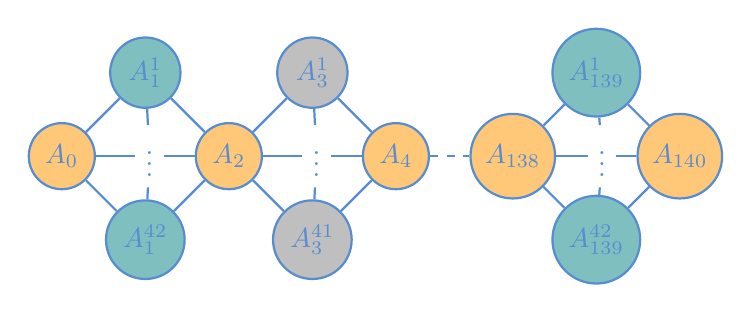
\begin{tikzpicture}[node distance={15mm}, thick, main/.style = {draw, circle}, cackithi] 
				\node[main, fill={rgb:orange,1;yellow,2;pink,5}] (1) {$A_0$}; 
				\node[main, fill= teal!50] (2) [above right of=1] {$A_1^1$}; 
				\node (3) [right = 5mm of 1] {$\vdots$};
				
				\node[main, fill= teal!50] (4) [below right of=1] {$A_1^{42}$}; 
				\node[main, fill={rgb:orange,1;yellow,2;pink,5}] (5) [below right of=2] {$A_2$}; 
				\node[main,fill=gray!50] (6) [above right of=5] {$A_3^1$}; 
				\node (7) [right = 5mm of 5] {$\vdots$};
				\node[main, fill=gray!50] (8) [below right of=5] {$A_3^{41}$}; 
				\draw (1) -- (2); 
				\draw (1) -- (3); 
				\draw (1) -- (4); 
				\draw (2) -- (3);
				\draw (3) -- (4);
				\draw (2) -- (5); 
				\draw (3) -- (5); 
				\draw (4) -- (5); 
				\draw (5) -- (6);
				\draw (5) -- (7);
				\draw (5) -- (8);   
				\draw (6) -- (7);
				\draw (7) -- (8);
				\node[main, fill={rgb:orange,1;yellow,2;pink,5}] (9) [below right of=6] {$A_4$};
				\draw (6) -- (9);
				\draw (7) -- (9); 
				\draw (8) -- (9);  
				\node[main, fill={rgb:orange,1;yellow,2;pink,5}] (10) [right = 5mm of 9] {$A_{138}$};
				\draw[dashed] (9) -- (10);  
				\node[main, fill= teal!50] (11) [above right of=10] {$A_{139}^1$}; 
				\node (12) [right = 4mm of 10] {$\vdots$}; 
				\node[main, fill= teal!50] (13) [below right of=10] {$A_{139}^{42}$}; 
				\draw (10) -- (11);
				\draw (10) -- (12);
				\draw (10) -- (13);
				\draw (11) -- (12);
				\draw (12) -- (13);
				\node[main, fill={rgb:orange,1;yellow,2;pink,5}] (14) [below right of=11] {$A_{140}$};
				\draw (11) -- (14);
				\draw (12) -- (14);
				\draw (13) -- (14);
			\end{tikzpicture}}
			\caption{\small\textit{\color{cackithi}Hình $1$. Hệ thống điểm quan sát với khoảng cách quan sát lớn nhất $140$. Mỗi điểm $A_i^{\bullet}$ thuộc tập $M_i$ có thể quan sát được tất cả điểm trong $M_{i-1}, M_{i+1}$ cũng như các điểm còn lại trong $M_i$.}}
			\vspace*{-10pt}
		\end{figure}
		\vskip 0.1cm		
		$\bullet$ Mỗi tập $M_{3k}$ và $M_{3k+2}$ với $k = 0, \ldots, 46$ chỉ chứa một điểm quan sát.
		\vskip 0.1cm
		$\bullet$ Mỗi tập $M_{1}$ và $M_{139}$ có $42$ điểm quan sát.
		\vskip 0.1cm
		$\bullet$ Mỗi tập $M_{3k+1}$ với $k = 1, \ldots, 45$ có $41$ điểm quan sát.
		\vskip 0.1cm
		Độc giả có thể kiểm tra rằng hệ thống này có $2023$ điểm quan sát và thỏa mãn điều kiện của bài toán. Ở đó, điểm quan sát duy nhất trong $M_{140}$ có khoảng cách quan sát $140$ tới điểm quan sát duy nhất trong $M_0$.
		\vskip 0.1cm
	\textbf{\color{cackithi}Câu $\pmb{3}$:} Cho tam giác $ABC$ với tâm đường tròn nội tiếp $I$. Gọi trung điểm của các cạnh $AC$ và $BC$ lần lượt là $M_b$ và $M_a$. Gọi giao điểm của đường thẳng $M_bI$ với đường thẳng $BC$ là $B'$ và giao điểm của đường thẳng $M_aI$ với đường thẳng $AC$ là $A'$. Biết rằng hai tam giác $ABC$ và $A'B'C$ có cùng diện tích. 
	\vskip 0.1cm
	Tìm giá trị có thể của góc $ACB$.\footnote{\color{cackithi}Trong số $09/2023$ chúng tôi đã sai sót khi yêu cầu tìm giá trị \textbf{\color{cackithi}lớn nhất} có thể của góc $ACB$. Thành thật xin lỗi các độc giả của Pi.}	
		\begin{figure}[H]
			\vspace*{-10pt}
			\centering
			\captionsetup{labelformat= empty, justification=centering}
			\resizebox{\columnwidth}{!}{\begin{tikzpicture}
				\tkzSetUpPoint[size=4,circle, fill= teal!50]
				\tkzDefPoints{0/0/A,6/0/B,0.8/4/C}
				
				\tkzDefTriangleCenter[centroid](A,B,C)
				\tkzGetPoint{G}
				\tkzDefSpcTriangle[medial](A,B,C){Ma,Mb,Mc}
				%\tkzLabelPoints(A,B,C)
				\tkzDefTriangleCenter[in](A,B,C)
				\tkzGetPoint{I}
				
				\tkzDefCircle[in](A,B,C) 
				\tkzGetPoints{I}{i}
				
				\tkzInterLL(Mb,I)(B,C)
				\tkzGetPoint{B1}
				\tkzInterLL(Ma,I)(A,C)
				\tkzGetPoint{A1}
				\tkzDrawSegments(A,B B,C C,A)
				\tkzDrawPoints(A1,B1)
				\tkzLabelPoint[above left](A1){$A'$}
				\tkzLabelPoint(B1){$B'$}
				\tkzDrawLines[dashed](B1,Mb A1,Ma)
				\tkzDrawSegments(B1,B A1,B1)
				\tkzDrawCircle(I,i)
				\tkzDrawPoints(I, Mb, Ma)
				
				\tkzDrawPoints(A,B,C)
				
				\tkzLabelPoint(I){$I$}
				
				\tkzLabelPoints[below left](A,Mb)
				\tkzLabelPoints[above right](B,Ma)
				\tkzLabelPoint[above](C){$C$}
			\end{tikzpicture}}
		\vspace*{-10pt}
		\end{figure}
		\textit{Lời giải.} Gọi độ dài các cạnh $AB$, $BC$ và $CA$ lần lượt là $c$, $a$, $b$. Đặt $\gamma \colon = \angle ACB$. Ta sẽ chứng minh rằng $\gamma = 60^{\circ}$.
		\vskip 0.1cm
		Thật vậy, từ $M_a$ vẽ đường thẳng song song với $AC$ và cắt $CI$ tại $P$. Vì $\angle CPM_a = \angle A'CI = \gamma/2$ nên tam giác $CM_aP$ cân tại $M_a$ và ta có $M_aP = M_aC = a/2 = M_aB$. Như vậy $P$ nằm trên đường tròn tâm $M_a$ bán kính $a/2$. Từ đó suy ra tam giác $BPC$ vuông tại $P$ và ta thu được 
		\begin{align*}
			CP = CB \cos (\gamma /2) = a \cos(\gamma/2).
		\end{align*}
		\begin{figure}[H]
			\vspace*{-5pt}
			\centering
			\resizebox{\columnwidth}{!}{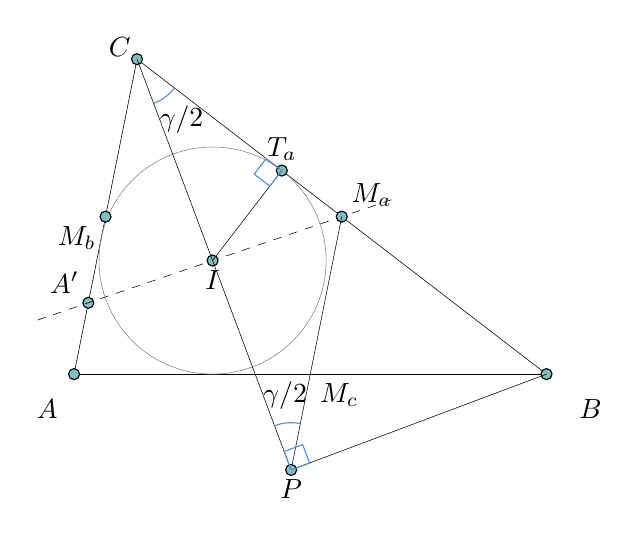
\begin{tikzpicture}[color= cackithi]
				\tkzSetUpPoint[size=4, fill= teal!50]
				
				\tkzDefPoints{0/0/A,6/0/B,0.8/4/C}
				
				\tkzDefTriangleCenter[centroid](A,B,C)
				\tkzGetPoint{G}
				\tkzDefSpcTriangle[medial](A,B,C){Ma,Mb,Mc}
				%\tkzLabelPoints(A,B,C)
				\tkzDefTriangleCenter[in](A,B,C)
				\tkzGetPoint{I}
				
				\tkzDefCircle[in](A,B,C) 
				\tkzGetPoints{I}{i}
				
				\tkzInterLL(Mb,I)(B,C)
				\tkzGetPoint{B1}
				\tkzInterLL(Ma,I)(A,C)
				\tkzGetPoint{A1}
				\tkzDrawSegments(A,B B,C C,A)
				\tkzDrawPoint(A1)
				\tkzLabelPoint[above left](A1){$A'$}
				\tkzDrawLine[dashed](A1,Ma)
				\tkzDrawCircle(I,i)
				\tkzDrawPoints(I, Mb, Ma)
				
				\tkzDrawPoints(A,B,C)
				
				\tkzLabelPoint(I){$I$}
				
				\tkzAutoLabelPoints[center = G](A,B,C)
				\tkzLabelPoint[below left](Mb){$M_b$}
				\tkzLabelPoint[above right](Ma){$M_a$}
				\tkzLabelPoint[below right](Mc){$M_c$}
				\tkzInterLL(C,I)(Ma,Mc)
				\tkzGetPoint{P}
				\tkzDrawSegments(C,P P,B Ma,P)
				\tkzDrawPoint(P)
				\tkzLabelPoint(P){$P$}
				\tkzDefPointBy[projection = onto C--B](I)
				\tkzGetPoint{Ta}
				\tkzDrawPoint(Ta)
				\tkzLabelPoint[above](Ta){$T_a$}
				\tkzDrawSegment(Ta,I)
				\tkzMarkRightAngles(C,Ta,I C,P,B)
				\tkzMarkAngle[size = 0.6, arc=l](P,C,B)
				\tkzLabelAngle[pos=0.95](P,C,B){$\gamma/2$}
				\tkzMarkAngle[size = 0.6, arc=l](Ma,P,C)
				\tkzLabelAngle[pos=0.95](Ma,P,C){$\gamma/2$}
			\end{tikzpicture}}
			\vspace*{-10pt}
		\end{figure}
		Gọi $T_a$ là điểm tiếp xúc của đường tròn nội tiếp tam giác $ABC$ với cạnh $BC$ thì $CT_a = (a+b-c)/2$. Do đó 
		\begin{align*}
			CI = \frac{CT_a}{\cos(\gamma/2)} = \frac{a+b-c}{2 \cos(\gamma/2)}
		\end{align*}
		và ta có
		\begin{align*}
		IP = CP - CI & =  a \cos(\gamma/2) - \frac{a+b-c}{2 \cos(\gamma/2)} \\
		& = \frac{2a \cos^2(\gamma/2) -a-b+c}{2 \cos(\gamma/2)} \\
		& = \frac{a[2\cos^2(\gamma /2)-1] - b +c}{2 \cos(\gamma/2)} \\
		& = \frac{a \cos (\gamma)-b+c}{2 \cos(\gamma/2)}.
		\end{align*}
		Vì $A'C \parallel M_aP$ nên theo định lý Thales 
		\begin{align*}
			\frac{CA'}{M_aP} = \frac{CI}{IP} & =  \frac{a+b-c}{a \cos(\gamma) - b +c} \\
			& = \frac{a+b-c}{a\frac{a^2 + b^2 -c^2}{2ab} -b +c} \\
			& = \frac{2b(a+b-c)}{a^2 + b^2 - c^2 - 2b^2 + 2bc} \\
			& = \frac{2b(a+b-c)}{a^2 - b^2 -c^2 + 2bc} \\
			& = \frac{2b(a+b-c)}{(a+c-b)(a+b-c)} \\
			& = \frac{2b}{a+c-b}
		\end{align*}
		và do đó
		\begin{align*} 
			\frac{CA'}{CB} = \frac{CA'}{2M_aP} = \frac{b}{a+c-b}. \tag{$3$}
		\end{align*}
		Hoán đổi vai trò của $A$ với $B$ (do đó $M_a$ với $M_b$, $a$ với $b$, $A'$ với $B'$) ta thu được
		\begin{align*} 
			\frac{CB'}{CA} = \frac{a}{b+c-a}. \tag{$4$}
		\end{align*}
		Từ giả thiết hai tam giác $ABC$ và $A'B'C$ có cùng diện tích ta có
		\begin{align*}
			\frac{CA'}{CB} = \frac{CA}{CB'}.
		\end{align*}
		Kết hợp với ($3$) và ($4$) ta nhận được
		\begin{align*}
			&\frac{b}{a+c-b}  = \frac{b+c-a}{a} \\
			\Leftrightarrow \,&ab  = (a+c-b)(b+c-a) \\
			\Leftrightarrow \,&ab  = c^2 - (a-b)^2 \\
			\Leftrightarrow \,&c^2 = a^2 + b^2 - ab.
		\end{align*}
		Từ hệ thức $c^2 = a^2 + b^2 - 2 ab \cos(\gamma)$ suy ra $\cos(\gamma) = \frac{1}{2}$. Do đó $\gamma = 60^{\circ}$.
	\vskip 0.1cm
	\textbf{\color{cackithi}Câu $\pmb{4}$}: Cho một đa giác đều $2n$ cạnh. Trong các đoạn thẳng nối các đỉnh của đa giác (cạnh biên hoặc đường chéo) ta tô $n$ đoạn màu đỏ sao cho:
	\vskip 0.1cm
	$1.$ Các điểm cuối của các đoạn màu đỏ chính là $2n$ đỉnh của đa giác.
	\vskip 0.1cm
	$2.$ Không có $2$ đoạn màu đỏ nào có độ dài bằng nhau.
	\vskip 0.1cm
	Tìm tất cả các số tự nhiên $n \ge 2$ sao cho tồn tại một phép tô màu thỏa mãn yêu cầu bên trên.
	\vskip 0.1cm	
	\textit{Lời giải.}
	Ta sẽ chứng minh rằng một cách tô màu như vậy tồn tại khi và chỉ khi $n \equiv 0 \mod 4$ hoặc $n \equiv 1 \mod 4$.
	\vskip 0.1cm
	$``\Rightarrow":$ Giả sử tồn tại cách tô màu như vậy. Gọi $2n$ đỉnh của đa giác là $A_1, A_2, \ldots, A_{2n}$, được sắp xếp theo chiều kim đồng hồ. Ta định nghĩa \textit{khoảng cách $d(i,j)$ giữa hai đỉnh $A_i, A_j$} là số cạnh nằm trên đường đi ngắn nhất dọc theo các cạnh biên của đa giác nối hai đỉnh này. Khoảng cách này sẽ lấy một trong các giá trị trong tập $\{1,2\ldots,n\}$. Chẳng hạn, với $n=4$ như trong Hình $2$ thì $d(1,4) = 3$ và $d(1,7) = 2$. 
	\vskip 0.1cm
	Dễ thấy
	\begin{align*}
		A_iA_j = 2r \sin\frac{d(i,j)\pi}{2n}
	\end{align*}
	với $r$ là khoảng cách từ đỉnh đến tâm của đa giác. Do đó, $A_iA_j > A_rA_s \iff d(i,j) > d(r,s)$. Bởi vậy ta có thể thay yêu cầu rằng không có hai đoạn màu đỏ nào có cùng độ dài bằng yêu cầu không có hai cặp đỉnh nào có cùng khoảng cách.
	\vskip 0.1cm	
	Biểu diễn mỗi cặp đỉnh $(A_i, A_j)$ bởi cặp chỉ số $(i,j)$. Ta có thể giả sử $i <j$. Bài toán đã cho tương đương với việc phân hoạch tập $2n$ số tự nhiên $\{1,2,\ldots, 2n\}$ thành $n$ cặp $\{(i_k,j_k)\}_{k = 1}^n$ với $i_k<j_k$ sao cho tập các khoảng cách $\{d(i_k,j_k)\}_{k=1}^n$ là $\{1, \ldots, n\}$. Ta có
	\begin{align*}
		\hspace*{-10pt}d(i_k,j_k) \!\!=\!\! 
		\begin{cases}
			\!\!j_k\!-\!i_k, \text{ nếu } j_k\!-\!i_k \!\le\! n \\
			\!\!2n\!-\! j_k \!+\! i_k, \text{ nếu } j_k\!-\!i_k \!>\! n.
		\end{cases}\hspace*{-10pt} \tag{$5$}
	\end{align*}
	Bằng cách hoán đổi $i_k$ với $j_k$ trong trường hợp $j_k-i_k > n$ ta có 
	\begin{align*} 
			\sum_{k=1}^{n}j_k - \sum_{k=1}^n i_k = &\sum_{k=1}^nd(i_k,j_k) + 2ns\\
			 = &\sum_{k=1}^ni + 2ns \\
			 = &n(n+1)/2 + 2ns.\tag{$6$}
		\end{align*}
		với $s$ là số trường hợp $j_k-i_k > n$. Mặt khác,
		\begin{align*}
			\sum_{k=1}^nj_k + \sum_{k=1}^ni_k &= \sum_{k=1}^{2n}i \\
			&= 2n(2n+1)/2. \tag{$7$}
		\end{align*}
		Từ các phương trình ($6$) và ($7$) ta thu được 
		\begin{align*}
			\sum_{k=1}^{n}j_k = \frac{n(5n+3)}{4} + ns.
		\end{align*}
		Vì $\sum_{k=1}^{n}j_k \in \mathbb{N}$ nên $\frac{n(5n+3)}{4} \in \mathbb{Z}$. Từ đó suy ra $n \equiv 0 \mod 4$ hoặc $n \equiv 1 \mod 4$.
		\vskip 0.1cm
		$``\Leftarrow":$
		\vskip 0.1cm
		\underline{\textit{Trường hợp $n \equiv 0 \mod 4$.}} Đặt $n = 4k$.
		\vskip 0.1cm
		$\bullet$ Với $k=1$ ta có thể tô màu như Hình $2$.
			\begin{figure}[H]
%				\vspace*{-10pt}
				\centering
				\captionsetup{labelformat= empty, justification=centering}
				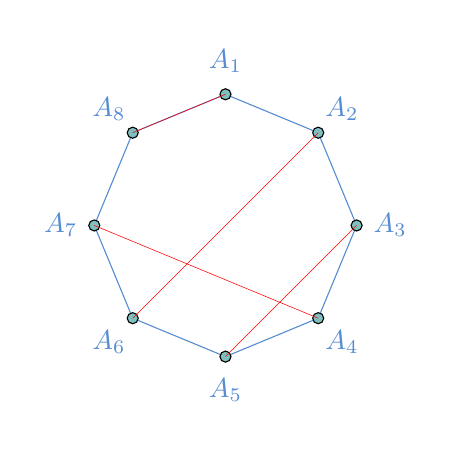
\begin{tikzpicture}[cackithi,scale = 0.75]
					\tkzSetUpPoint[size=4, fill= teal!50]
					\def\laenge{1.7}
					\def\n{8}
					\pgfmathtruncatemacro\w{360/\n}
					\draw
					(0:0) coordinate (A1)
					foreach \i in {2,...,\n}
					{--++(360+\w/2-\i*\w +\w:\laenge) coordinate (A\i)}
					--cycle;
					\tkzDrawPoints(A1,A...,A8)
					\foreach \i in {1,...,\n}\node[anchor={270-\i*\w +\w}, circle] at (A\i){$A_{\i}$};
					\tkzDrawSegment[red](A1,A8)
					\tkzDrawSegment[red](A2,A6)
					\tkzDrawSegment[red](A3,A5)
					\tkzDrawSegment[red](A4,A7)
				\end{tikzpicture}
				\caption{\small\textit{\color{cackithi}Hình $2$. Đa giác đều $8$ cạnh.}}
				\vspace*{-10pt}
			\end{figure}
			$\bullet$ Với $k \ge 2$ thì danh sách các đoạn màu đỏ cùng với khoảng cách giữa các đỉnh (phương trình ($5$) với $2n = 8k$) được cho trong bảng dưới đây:
		\begin{center}
			\resizebox{\linewidth}{!}{%
				\begin{tabular}{ |c|c|c| } 
					\hline
					Chỉ số & Cạnh & Khoảng cách \\ 
					\hline
					$1 \le i \le k$ & $(i, 8k+1-i)$ & $1,3, \ldots, 2k-1$ \\ 
					\hline
					$i = k+1$ & $(k+1, 5k+1)$ & $4k$ \\
					\hline
					$k+2 \le i \le 2k$ & $(i, 8k+2-i)$ & $2k+2, 2k+4, \ldots, 4k-2$ \\ 
					\hline
					$i = 2k+1$ & $(2k+1,4k+1)$ & $2k$ \\
					\hline
					$2k+2 \le i \le 3k+1$ & $(i, 8k+3-i)$ & $4k-1, 4k-3,\ldots, 2k+1$ \\
					\hline
					$3k+2 \le i \le 4k$ & $(i, 8k+2-i)$ & $2k-2, \ldots, 2$ \\
					\hline
			\end{tabular}}
		\end{center}
		\begin{figure}[H]
%			\vspace*{-5pt}
			\centering
			\captionsetup{labelformat= empty, justification=centering}
			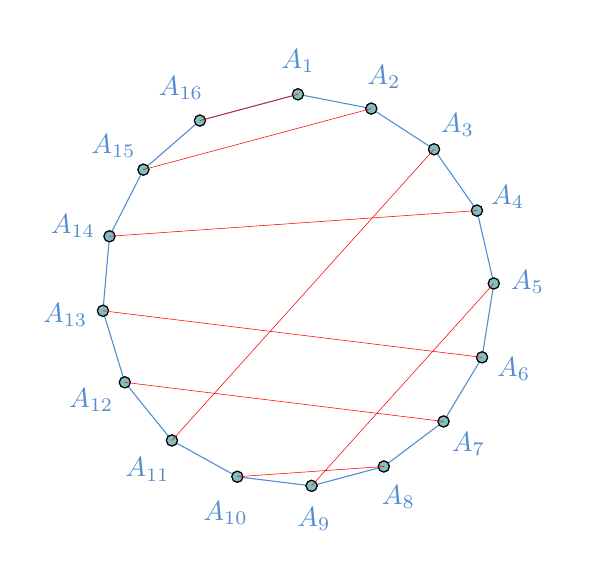
\begin{tikzpicture}[cackithi,scale = 0.95]
				\tkzSetUpPoint[size=4, fill= teal!50]
				\def\laenge{1}
				\def\n{16}
				\pgfmathtruncatemacro\w{360/\n}
				\draw
				(0:0) coordinate (A1)
				foreach \i in {2,...,\n}
				{--++(360+\w/2-\i*\w +\w:\laenge) coordinate (A\i)}
				--cycle;
				\tkzDrawPoints(A1,A...,A16)
				\foreach \i in {1,...,\n}\node[anchor={270-\i*\w +\w}, circle] at (A\i){$A_{\i}$};
				\tkzDrawPoints(A1,A...,A16)
				\tkzDrawSegment[red](A1,A16)
				\tkzDrawSegment[red](A2,A15)
				\tkzDrawSegment[red](A3,A11)
				\tkzDrawSegment[red](A4,A14)
				\tkzDrawSegment[red](A5,A9)
				\tkzDrawSegment[red](A6,A13)
				\tkzDrawSegment[red](A7,A12)
				\tkzDrawSegment[red](A8,A10)
			\end{tikzpicture}
			\caption{\small\textit{\color{cackithi}Hình $3$. Đa giác đều $16$ cạnh.}}
			\vspace*{-15pt}
		\end{figure}
		\underline{\textit{Trường hợp $n \equiv 1 \mod 4$.}} Đặt $n = 4k+1$. 
		\vskip 0.1cm
		$\bullet$ Với $k=1$ ta có thể tô màu như Hình $4$.
		\begin{figure}[H]
			\vspace*{-10pt}
			\centering
			\captionsetup{labelformat= empty, justification=centering}
			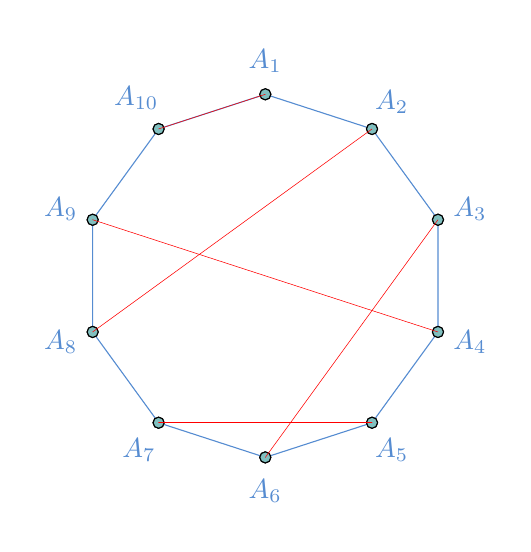
\begin{tikzpicture}[cackithi,scale = 0.95]
				\tkzSetUpPoint[size=4, fill= teal!50]
				\def\laenge{1.5}
				\def\n{10}
				\pgfmathtruncatemacro\w{360/\n}
				\draw
				(0:0) coordinate (A1)
				foreach \i in {2,...,\n}
				{--++(360+\w/2-\i*\w +\w:\laenge) coordinate (A\i)}
				--cycle;
				\tkzDrawPoints(A1,A...,A10)
				\foreach \i in {1,...,\n}\node[anchor={270-\i*\w +\w}, circle] at (A\i){$A_{\i}$};
				\tkzDrawPoints(A1,A...,A10)
				\tkzDrawSegment[red](A1,A10)
				\tkzDrawSegment[red](A2,A8)
				\tkzDrawSegment[red](A3,A6)
				\tkzDrawSegment[red](A4,A9)
				\tkzDrawSegment[red](A5,A7)
			\end{tikzpicture}
			\caption{\small\textit{\color{cackithi}Hình $4$. Đa giác đều $10$ cạnh.}}
			\vspace*{-15pt}
		\end{figure}
		$\bullet$  Với $k \ge 2$ thì danh sách các đoạn màu đỏ cùng với khoảng cách giữa các đỉnh (phương trình ($5$) với $2n = 8k+2$) được cho trong bảng dưới đây:
		\begin{center}
			\resizebox{\linewidth}{!}{%
				\begin{tabular}{ |c|c|c| } 
					\hline
					Chỉ số & Cạnh & Khoảng cách \\ 
					\hline
					$1 \le i \le k$ & $(i, 8k+3-i)$ & $1,3, \ldots, 2k-1$ \\ 
					\hline
					$i = k+1$ & $(k+1, 5k+3)$ & $4k$ \\
					\hline
					$k+2 \le i \le 2k$ & $(i, 8k+4-i)$ & $2k+2, 2k+4, \ldots, 4k-2$ \\ 
					\hline
					$i = 2k+1$ & $(2k+1, 4k+2)$ & $2k+1$ \\
					\hline
					$2k+2 \le i \le 3k+1$ & $(i, 8k+5-i)$ & $4k+1, 4k-1,\ldots, 2k+3$ \\
					\hline
					$3k+2 \le i \le 4k+1$ & $(i,8k+4-i)$ & $2k, \ldots, 2$ \\
					\hline
			\end{tabular}}
		\end{center}
\end{multicols}
\newpage
\begingroup
\AddToShipoutPicture*{\put(150,700){\includegraphics[scale=1]{../tieude1.pdf}}}
\centering
\endgroup
\vspace*{3pt}

\begin{multicols}{2}
	Trong phần đầu chuyên mục, chúng tôi sẽ trình bày với các bạn lời giải các bài toán trong kỳ thi Olympic toán Tuymaada năm $2022$ của nước cộng hòa Sakha (Yakutia), thuộc Liên bang Nga đăng trong số tháng $5/2023$. 
	\begin{figure}[H]
		\vspace*{-5pt}
		\centering
		\captionsetup{labelformat= empty, justification=centering}
		\includegraphics[width= 1\linewidth]{gocolympic}
%		\caption{\small\textit{\color{}.}}
		\vspace*{-15pt}
	\end{figure}
	{\bf\color{cackithi} OC$\pmb{46.}$} Arnim và Brentano có một chiếc bình nhỏ đựng $1500$ viên kẹo trên bàn và một túi lớn đựng kẹo dự phòng dưới gầm bàn. Họ thay phiên nhau chơi một trò chơi với Arnim bắt đầu trước. Ở mỗi lượt đi, người chơi có thể ăn $7$ viên kẹo trong bình hoặc lấy 6 viên kẹo từ túi bên dưới và thêm chúng vào bình. Người chơi không được lấy kẹo trong túi dưới gầm bàn hai lần liên tiếp. Người chơi được tuyên bố là người chiến thắng nếu làm cho chiếc bình rỗng sau lượt chơi của mình. Trong mọi trường hợp khác, nếu
	một người chơi không thể thực hiện được nước đi trong lượt của mình, trò chơi được tuyên bố là hòa. Liệu người nào có chiến lược để luôn chiến thắng?
	\vskip 0.1cm
	\textit{Lời giải.} Ban đầu trong bình có $1500$ viên kẹo. Brentano có chiến lược để luôn thắng bằng cánh đảm bảo rằng nếu trước lượt đi của Arnim trong bình có $15k$ viên kẹo, thì sau khi mỗi người đi $2$ lượt, trong bình sẽ còn lại $15(k-1)$ viên kẹo. 
	\vskip 0.1cm
	Cụ thể là nếu trong lượt đi thứ nhất của mình Arnim thêm $6$ viên kẹo vào bình thì ở lượt đi sau anh ta phải ăn $7$ viên. Do đó Brentano sẽ ăn $7$ viên kẹo trong cả $2$ lượt đi của mình và số kẹo trong bình sau đó là $15k+6-7-7-7=15(k-1).$ Nếu trong lượt đi thứ nhất của mình Arnim  ăn $7$ viên thì Brentano cũng ăn $7$ viên trong lượt thứ nhất. 
	Đến lượt đi thứ $2$ nếu Arnim ăn $7$ viên thì sau đó Brentano thêm vào $6$ viên và số kẹo trong bình còn lại là $15k-7-7-7+6=15(k-1).$    Còn nếu đến lượt thứ $2$ Arnim thêm vào 6 viên thì sau đó Brentano sẽ ăn $7$ viên và số kẹo trong bình còn lại là $15k-7-7+6-7=15(k-1).$ Như vậy sau khi mỗi người đi $200$ lượt thì Brentano là người chiến thắng.
	\vskip 0.1cm
	{\bf\color{cackithi}OC$\pmb{47.}$}  Cho $M$ là trung điểm của cạnh $A$B trong tam giác đều $ABC.$ Điểm $D$ thuộc cạnh $BC$ sao cho $BD : DC = 3 : 1.$ Giả sử $T$ là điểm trên đường thẳng đi qua $C$ và song song với $MD$ sao cho $\angle CTA = 150^\circ.$ Tìm số đo $\angle MTD.$
	\begin{figure}[H]
		\vspace*{-5pt}
		\centering
		\captionsetup{labelformat= empty, justification=centering}
		\definecolor{qqwuqq}{rgb}{0.,0.39215686274509803,0.}
		\definecolor{uuuuuu}{rgb}{0.26666666666666666,0.26666666666666666,0.26666666666666666}
		\definecolor{ududff}{rgb}{0.30196078431372547,0.30196078431372547,1.}
		\begin{tikzpicture}[cackithi,scale=1.2,node font=\small]
			\draw[color=uuuuuu] (1.8771681255350392,1.9481399025612232) -- (1.90851486019539,2.1110223138105475) -- (1.7456324489460657,2.1423690484708984) -- (1.7142857142857149,1.979486637221574) -- cycle; 
			\draw [shift={(1.7142857142857149,1.979486637221574)},color=qqwuqq,fill=qqwuqq,fill opacity=0.10000000149011612] (0,0) -- (-130.8933946491309:0.23457748258628952) arc (-130.8933946491309:-10.893394649130876:0.23457748258628952) -- cycle;
			\draw  (2.,0.) circle (2.cm);
			\draw  (2.,3.4641016151377553)-- (2.5,2.5980762113533165);
			\draw  (2.3109450177226596,3.0662755356334794) -- (2.1890549822773426,2.9959022908575927);
			\draw  (3.,1.7320508075688776)-- (2.5,2.5980762113533165);
			\draw  (2.689054982277343,2.129876887073154) -- (2.8109450177226605,2.2002501318490406);
			\draw  (3.,1.7320508075688776)-- (3.5,0.8660254037844388);
			\draw  (3.3109450177226583,1.3342247280646016) -- (3.1890549822773413,1.263851483288715);
			\draw  (3.5,0.8660254037844388)-- (4.,0.);
			\draw  (3.8109450177226587,0.4681993242801627) -- (3.6890549822773417,0.3978260795042762);
			\draw  (0.,0.)-- (2.,0.);
			\draw  (0.9706778146767137,0.07037324477588658) -- (0.9706778146767137,-0.07037324477588658);
			\draw  (1.029322185323286,0.07037324477588658) -- (1.029322185323286,-0.07037324477588658);
			\draw  (2.,0.)-- (4.,0.);
			\draw  (2.9706778146767134,0.07037324477588658) -- (2.9706778146767134,-0.07037324477588658);
			\draw  (3.0293221853232857,0.07037324477588658) -- (3.0293221853232857,-0.07037324477588658);
			\draw  (2.5,2.5980762113533165)-- (2.,0.);
			\draw  (3.,1.7320508075688776)-- (2.,0.);
			\draw  (2.5756061103843018,0.8562325387809366) -- (2.453716074938985,0.9266057835568232);
			\draw  (2.5462839250610156,0.8054450240120545) -- (2.4243938896156987,0.8758182687879411);
			\draw  (1.7142857142857149,1.979486637221574)-- (3.,1.7320508075688776);
			\draw  (2.,3.4641016151377553)-- (1.7142857142857149,1.979486637221574);
			\draw  (1.7142857142857149,1.979486637221574)-- (0.,0.);
			\draw  (2.,0.)-- (1.7142857142857149,1.979486637221574);
			\draw  (1.7916802919345747,0.9506685609177279) -- (1.9309831895863658,0.9707752022822663);
			\draw  (1.7833025246993495,1.0087114349393076) -- (1.9226054223511404,1.0288180763038461);
			\draw  (1.7142857142857149,1.979486637221574)-- (2.5,2.5980762113533165);
			\draw  (2.0636107016266734,2.3440746880399277) -- (2.1506750126590424,2.233488160534963);
%			\begin{scriptsize}
				\draw [fill=white] (0.,0.) circle (1.5pt);
				\draw[color=ududff] (-0.17754689709133267,-0.15347137061022087) node {$A$};
				\draw [fill=white] (4.,0.) circle (1.5pt);
				\draw[color=ududff] (4.23250977553091,-0.16520024473953532) node {$B$};
				\draw [fill=white] (2.,3.4641016151377553) circle (1.5pt);
				\draw[color=uuuuuu] (2.086125809866361,3.6818704696755975) node {$C$};
				\draw [fill=white] (2.,0.) circle (1.5pt);
				\draw[color=uuuuuu] (2.0157525650904744,-0.21211574125679306) node {$M$};
				\draw [fill=white] (3.,1.7320508075688776) circle (1.5pt);
				\draw[color=uuuuuu] (3.1769111038926074,1.922539350278433) node {$R$};
				\draw [fill=white] (2.5,2.5980762113533165) circle (1.5pt);
				\draw[color=uuuuuu] (2.649111768073456,2.8022049099770157) node {$D$};
				\draw [fill=white] (3.5,0.8660254037844388) circle (1.5pt);
				\draw[color=uuuuuu] (3.3763019640909535,0.6558209443124747) node {$F$};
				\draw [fill=white] (1.7142857142857149,1.979486637221574) circle (1.5pt);
				\draw[color=uuuuuu] (1.5935130964351534,2.1688457069940363) node {$R'$};
				\draw (2.2386011735474494,1.7700639865973455) node[below] {$120^{\circ}$};
%			\end{small}
		\end{tikzpicture}
		\vspace*{-5pt}
	\end{figure}
	\textit{Lời giải.} Gọi $\ell$ là đường thẳng đi qua $C$ song song với $MD.$ Giả sử đường tròn đường kính $AB$ cắt $BC$ tại $R$ và cắt $\ell$ tại $R'.$  Ta sẽ chứng minh  $R'$ trùng với  $T.$ 
	\vskip 0.1cm
	Dễ thấy tam giác cân $MBR$ có góc $\angle MBR=60^\circ$ nên nó là tam giác đều. Do đó $R$ là trung điểm $BC$ và $D$ là trung điểm $RC.$ Trong tam giác $CRR',$ $MD$ đi qua trung điểm của $CR$ và song song $CR'$ nên nó phải đi qua trung điểm của $RR'.$ Do $MD$ là đường kính, ta suy ra $MD\perp RR'.$ Do $CR'$ song song với $MD,$ ta suy ra $\angle CR'R=90^\circ.$ 
	\vskip 0.1cm
	Mặt khác, do $\angle AR'R=180^\circ - \angle ABR= 180^\circ-60^\circ=120^\circ,$ ta có 
	\begin{align*}
		\angle AR'C&=360^\circ-\angle AR'R - \angle CR'R \\
		&= 360^\circ -120^\circ - 90^\circ=150^\circ.
	\end{align*}
	Như vậy $R'$ trùng với $T.$ Do $R$ và $R'$ đối xứng nhau qua $MD$ ta có $\angle MR'D=\angle MRD= 120^\circ.$  Như vậy $\angle MTD=120^\circ.$  
	\vskip 0.1cm
	{\bf\color{cackithi} OC$\pmb{48.}$} Cho các số nguyên $a, b, c$ và số nguyên tố lẻ $p.$ Chứng minh rằng tồn tại các số nguyên $x$ và $y$ sao cho $p$ là ước của $x^2 + y^2 + ax + by + c.$      
	\vskip 0.1cm
	\textit{Lời giải.}
	Khi tính giá trị  $f(x)=x^2+ax+c$ modulo $p,$ với $x \in \{0, 1, \cdots, p - 1\}$ ta được ít nhất $\frac{p+1}{2}$  số phân biệt. Thật vậy, nếu $x_1$ và $x_2$ là hai số nguyên phân biệt nằm giữa $0$ và $p-1$, và $p$ là ước của  $f(x_1)-f(x_2) = x_1^2 +ax_1+c-(x_2^2 +ax_2+c) = (x_1-x_2)(x_1+x_2+a)$,
	thì $p$ cũng là ước của $x_1 + x_2 + a$, nghĩa là với mỗi $x_1\in \{0, 1, \cdots, p - 1\}$ có nhiều nhất
	một $x_2\in \{0, 1, \cdots, p - 1\}$  sao cho $f(x_2)\equiv f(x_1) \mod p.$ 
	\vskip 0.1cm
	Lập luận tương tự cho thấy các giá trị của đa thức $g(y) = -y^2 - by$ với  $y \in \{0, 1, \cdots, p - 1\}$ ta cũng nhận được ít nhất $\frac{p+1}{2}$ số phân biệt modulo $p.$ Như vậy, ta có hai tập các số dư modulo $p,$  mỗi tập có nhiều hơn $\frac{p}{2}$ số dư, do đó hai tập này phải có ít nhất một phần tử chung. Ta suy ra $p$ là ước của $f(x) - g(y)$ với các số nguyên $x$ và $y$ nào đó. Ta được điều cần chứng minh.  
	\vskip 0.1cm
	Trong phần cuối của chuyên mục kỳ này, chúng tôi sẽ giới thiệu với bạn đọc ba bài toán chọn lọc trong kỳ thi Olympic toán vùng Trung Mỹ và Caribê năm $2023$. Các bài toán này phù hợp với trình độ học sinh lớp $8-10$.
	\vskip 0.1cm
	{\bf\color{cackithi} OC$\pmb{55.}$} Tìm tất cả các cách tô màu các số nguyên dương sao cho điều kiện sau thỏa mãn:  
	\vskip 0.1cm
	$\bullet$ Mỗi số có màu xanh hoặc đỏ;
	\vskip 0.1cm
	$\bullet$ Tổng của hai số (không nhất thiết phân biệt) cùng màu bất kỳ  có màu xanh.
	\vskip 0.1cm
	{\bf\color{cackithi} OC$\pmb{56.}$} Octavio viết một số nguyên dương $n$ lên bảng  và sau đó anh bắt đầu một quá trình trong đó, ở mỗi bước, anh xóa số nguyên $k$ được viết trên bảng  và thay thế nó bằng một trong các số sau:
	\begin{align*}
		3k-1, \quad 2k+1, \quad \frac{k}{2},
	\end{align*}
	với điều kiện số mới viết là số nguyên.
	\vskip 0.1cm
	Chứng minh rằng với mọi số nguyên dương $n$, Octavio có thể viết lên bảng  số $3^{2023}$ sau hữu hạn bước.
	\vskip 0.1cm
	{\bf\color{cackithi} OC$\pmb{57.}$} Trong một cái ao có $n (n \geq 3)$  hòn đá  xếp thành vòng tròn. Một công chúa muốn đánh số những hòn đá với các số $1, 2, \dots, n$ theo thứ tự nào đó rồi đặt một số con cóc lên những hòn đá. Sau khi đặt tất cả các con cóc vào vị trí, chúng bắt đầu nhảy theo quy tắc sau: khi một con cóc đến hòn đá có đánh số $k$, nó đợi $k$ phút rồi nhảy sang hòn đá liền kề theo chiều kim đồng hồ.
	\vskip 0.1cm
	Hỏi số lượng cóc nhiều nhất là bao nhiêu để công chúa có thể đánh số các hòn đá và đặt các con cóc sao cho không bao giờ có hai con cóc ở trên cùng một hòn đá trong thời gian từ một phút trở lên?
\end{multicols}
	\newpage

	\setcounter{figure}{0}
	\thispagestyle{lichsutoanhocnone}
\pagestyle{lichsutoanhoc}
\graphicspath{{../lichsutoanhoc/pic/}}
\everymath{\color{lichsutoanhoc}}
\blfootnote{$^*$\color{lichsutoanhoc}Dịch theo https://mathshistory.st-andrews.ac.uk/Biographies/Noether\_Emmy/}
\blfootnote{$^1$\color{lichsutoanhoc}Đại học Sư phạm Hà Nội.}
\begingroup
\AddToShipoutPicture*{\put(0,616){\includegraphics[width=19.3cm]{../bannerlichsu}}}
\AddToShipoutPicture*{\put(78,552){\includegraphics[scale=1]{../tieude4.pdf}}}
\centering
\endgroup

\vspace*{160pt}

	``\textit{Phương pháp của tôi, quả thật là phương pháp của làm việc và suy nghĩ, 
	đó chính là lý do vì sao chúng len lỏi vào mọi nơi trong cuộc sống một cách ẩn danh}."
\begin{multicols}{2}
		\begin{figure}[H]
%		\vspace*{5pt}
		\centering
		\captionsetup{labelformat= empty, justification=centering}
		\includegraphics[width= 0.45\linewidth]{1a}
		\caption{\small\textit{\color{lichsutoanhoc}Emmy Amalie Noether ($1882-1935$).}}
		\vspace*{-10pt}
	\end{figure}
	Cha của Emmy Noether, Max Noether, là một nhà toán học nổi tiếng và là giáo sư tại Erlangen nhưng ông xuất thân từ một gia đình buôn bán đồ sắt thép. Mẹ cô là Ida Amalia Kaufmann ($1852-1915$), xuất thân từ một gia đình giàu có ở Cologne. Cha mẹ của Emmy đều có nguồn gốc Do Thái và người đọc có thể ngạc nhiên về điều này vì Noether không phải là tên Do Thái. Do đó, chúng ta nên giải thích điều này đã xảy ra như thế nào, đồng thời đưa ra một số thông tin về tổ tiên của Emmy Noether. Ông nội của Max Noether là Elias Samuel, người sáng lập một doanh nghiệp ở Bruchsal. Elias có chín người con,  một người con trai trong số đó là  Hertz Samuel. Năm $1809$, bang Baden ban hành Sắc lệnh Khoan dung yêu cầu người Do Thái lấy tên tiếng Đức. Elias Samuel chọn họ Nöther, trở thành Elias Nöther, nhưng cũng đổi tên các con mình, đặt cho Hertz cái tên Hermann. Khi được mười tám tuổi, Hermann Nöther rời quê hương Bruchsal và theo học thần học tại Đại học Mannheim. Sau đó vào năm $1837$, cùng với anh trai Joseph, ông thành lập một cơ sở kinh doanh bán buôn đồ sắt. Hermann Nöther và vợ Amalia có năm người con, người thứ ba là Max. Hai đứa trẻ lớn hơn Max là Sarah (sinh ngày $6$ tháng $11$ năm $1839$) và Emil. Điều đáng lưu ý ở điểm này là doanh nghiệp bán buôn sắt Nöther vẫn là một công ty gia đình trong đúng một trăm năm, cho đến khi Đức Quốc xã loại bỏ các gia đình Do Thái khỏi hoạt động kinh doanh của chính họ vào năm $1937$. Ta có một lưu ý cần thiết ở điểm này. Mặc dù họ của Max được ông nội của Max chọn là Nöther nhưng Max và gia đình ông  luôn sử dụng dạng Noether (ngoại trừ trên giấy chứng nhận đám cưới của Max có xuất hiện dạng Nöther).
	\vskip 0.05cm
	Emmy là con cả trong gia đình có bốn người con, ba người em nhỏ hơn là đều là con trai. Alfred Noether ($1883-1918$) nghiên cứu hóa học và nhận bằng tiến sỹ tại Erlangen năm $1909$. Tuy nhiên, sự nghiệp của ông rất ngắn ngủi vì ông qua đời $9$ năm sau đó. Fritz Noether ($1884-1941$) trở thành nhà toán học ứng dụng. Tuy nhiên, là một người Do Thái, ông không thể làm việc và phải rời nước Đức vào năm $1937$. Ông được bổ nhiệm làm giáo sư tại Đại học Tomsk ở Liên Xô nhưng bị buộc tội có hành động chống nhà nước  Xô Viết, ông bị kết án tử hình và bị xử bắn. Ông được Tòa án Tối cao Liên Xô tuyên vô tội vào năm $1988$. Gustav Robert Noether ($1889-1928$) suốt đời có sức khỏe kém. Ông bị thiểu năng trí tuệ, dành phần lớn cuộc đời trong viện dưỡng lão và chết trẻ. Ngôi trường đầu tiên Emmy theo học là ở Fahrstrasse. Auguste Dick viết trong [$2$]:
	\vskip 0.05cm
	\textit{Emmy không có vẻ gì đặc biệt khi còn nhỏ. Chơi đùa cùng các bạn trong sân trường ở Fahrstrasse, có lẽ cô ấy không đặc biệt đáng chú ý -- một cô bé cận thị, có vẻ ngoài giản dị, mặc dù không phải là không có duyên. Các giáo viên và bạn cùng lớp của cô biết đến Emmy như một đứa trẻ thông minh, thân thiện và dễ mến. Cô ấy nói hơi ngọng và là một trong số ít người tham gia các lớp học về đạo Do Thái.}
	\vskip 0.05cm
	Sau khi học tiểu học, Emmy Noether theo học tại Städtische Höhere Töchter Schule trên Friedrichstrasse ở Erlangen từ năm $1889$ đến năm $1897$. Cô sinh ra trong ngôi nhà gia đình ở Hauptstrasse $23$ và sống ở đó cho đến giữa thời gian học trung học, vào năm $1892$, gia đình chuyển đến một căn hộ lớn hơn ở Nürnberger Strasse $32$. Ở trường trung học, cô học tiếng Đức, tiếng Anh, tiếng Pháp, số học và được học piano. Cô thích khiêu vũ và mong chờ những bữa tiệc cùng con cái của các đồng nghiệp đại học của cha cô. Ở giai đoạn này, mục tiêu của cô là trở thành một giáo viên ngôn ngữ và sau khi học thêm tiếng Anh và tiếng Pháp, cô đã tham gia các kỳ thi của bang Bavaria và vào năm $1900$, cô trở thành giáo viên được cấp chứng chỉ dạy tiếng Anh và tiếng Pháp tại các trường nữ sinh ở Bavaria. Cô được điểm ``rất giỏi" trong các kỳ thi, mảng yếu nhất lại là việc giảng dạy trên lớp của cô.
	\vskip 0.05cm
	Tuy nhiên Noether chưa bao giờ trở thành giáo viên ngôn ngữ. Thay vào đó, cô quyết định đi theo con đường khó khăn đối với một phụ nữ thời đó và học toán ở trường đại học. Phụ nữ được phép học tại các trường đại học Đức một cách không chính thức và mỗi giáo sư phải cấp phép cho khóa học của mình. Noether được phép tham gia các khóa học tại Đại học Erlangen trong thời gian từ $1900$ đến $1902$. Cô là một trong hai sinh viên nữ duy nhất tham gia các khóa học tại Erlangen và, ngoài các khóa học toán, cô tiếp tục quan tâm đến các ngôn ngữ được dạy bởi một giáo sư về La Mã học và bởi một nhà sử học. Đồng thời, cô cũng chuẩn bị tham gia một kỳ thi cho phép sinh viên vào bất kỳ trường đại học nào. Sau khi vượt qua kỳ thi trúng tuyển ở Nürnberg vào ngày $14$ tháng $7$ năm $1903$, cô đã đến Đại học Göttingen. Trong thời gian $1903-04$, cô đã tham dự các bài giảng của Karl Schwarzschild, Otto Blumenthal, David Hilbert, Felix Klein và Hermann Minkowski. Một lần nữa, cô không được phép trở thành một sinh viên trúng tuyển chính thức mà chỉ được phép ngồi giảng bài. Sau một học kỳ tại Göttingen, cô trở lại Erlangen.
	\vskip 0.05cm
	Tại thời điểm này, các quy tắc đã được thay đổi và học sinh nữ được phép trúng tuyển trên cơ sở bình đẳng với nam giới. Ngày $24$ tháng $10$ năm $1904$, Noether trúng tuyển tại Erlangen, nơi bây giờ cô chỉ học toán. Năm $1907$, cô được cấp bằng tiến sỹ sau khi làm việc dưới sự hướng dẫn của Paul Gordan. Bài kiểm tra miệng diễn ra vào thứ Sáu ngày $13$ tháng $12$ và cô đã được trao bằng ``summa cum laude". Định lý cơ bản của Hilbert năm $1888$ đã đưa ra kết quả tồn tại tính hữu hạn của các bất biến trong $n$ biến. Tuy nhiên, Gordan đã áp dụng cách tiếp cận mang tính xây dựng và xem xét các phương pháp mang tính xây dựng để đạt được kết quả tương tự. Luận án tiến sỹ của Noether tuân theo cách tiếp cận mang tính xây dựng này của Gordan và liệt kê các hệ thống gồm $331$ dạng hiệp biến. Colin McLarty viết trong [$4$] rằng
	\vskip 0.05cm
	\textit{Luận án của cô năm $1908$ với Gordan theo đuổi một phép tính khổng lồ đã từng làm Gordan bối rối bốn mươi năm trước và ngay cả Noether cũng không thể hoàn thành được. Theo như tôi biết thì chưa có ai từng hoàn thành nó hoặc thậm chí đã từng kiểm tra nó như cô ấy đã làm. Vào thời điểm đó, nó đã lỗi thời, là một nhân chứng cho sự cô lập dễ chịu của Erlangen và  nó đã không tận dụng được công trình của chính Gordan xây dựng dựa trên ý tưởng của Hilbert.}
	\vskip 0.05cm
	Sau khi hoàn thành bằng tiến sỹ, quá trình bình thường để đạt được một vị trí học thuật sẽ là luận án tiến sỹ khoa học. Tuy nhiên con đường này không dành cho phụ nữ nên Noether vẫn ở lại Erlangen, giúp đỡ cha cô, một người đặc biệt vì sự ốm yếu bệnh tật của mình nên rất biết ơn sự giúp đỡ của con gái ông. Noether cũng thực hiện nghiên cứu của riêng mình, đặc biệt là cô chịu ảnh hưởng của Ernst Fischer, người kế nhiệm Gordan làm trưởng khoa toán học khi ông nghỉ hưu năm $1911$. Noether viết về ảnh hưởng của Fischer:
	\vskip 0.05cm
	\textit{Trên hết, tôi mang ơn ông E. Fischer, người đã thúc đẩy tôi nghiên cứu đại số trừu tượng từ quan điểm số học, và đây vẫn là ý tưởng chủ đạo cho tất cả công việc sau này của tôi.}
	\vskip 0.05cm
	Ảnh hưởng của Fischer đã đưa Noether hướng tới cách tiếp cận trừu tượng của Hilbert đối với chủ đề này và tránh xa cách tiếp cận mang tính xây dựng của Gordan. Điều này rất quan trọng đối với sự phát triển của cô với tư cách là một nhà toán học bởi  Gordan, mặc dù có những thành tựu đáng chú ý nhưng cũng có những hạn chế của ông. Cha của Noether, Max Noether, nói về Gordan (xem [$1$]):
	\vskip 0.05cm
	\textit{Gordan không bao giờ có thể đánh giá đúng sự phát triển của các khái niệm cơ bản; ngay cả trong các bài giảng của mình, ông ấy đã hoàn toàn tránh xa mọi định nghĩa cơ bản về bản chất khái niệm, thậm chí cả định nghĩa về giới~hạn.}
	\vskip 0.05cm
	Danh tiếng của Noether tăng lên nhanh chóng khi các ấn phẩm của cô xuất hiện. Năm $1908$, cô được bầu vào Circolo Matematico di Palermo, sau đó vào năm $1909$, cô được mời trở thành thành viên của Deutsche Mathematiker--Vereinigung và cùng năm đó, cô được mời phát biểu tại cuộc họp thường niên của Hiệp hội ở Salzburg. Cô đã giảng bài \textit{Zur Invariantentheorie der Formen von $n$ Variabeln}. Năm $1913$, cô giảng dạy ở Vienna, một lần nữa tại một cuộc họp của Deutsche Mathematiker--Vereinigung. Bài giảng của cô trong dịp này là \textit{Über Reasone Funktionenkörper}. Khi ở Vienna cô đã đến thăm Franz Mertens và trao đổi thảo luận về toán học với ông. Một trong những người cháu trai của Mertens nhớ lại chuyến viếng thăm của Noether (xem [$2$]):
	\vskip 0.05cm
	\textit{\ldots mặc dù là một phụ nữ, nhưng đối với tôi [cô ấy] có vẻ giống như một tuyên úy Công giáo đến từ một giáo xứ nông thôn -- mặc một chiếc áo khoác màu đen, dài gần đến mắt cá chân và trông không có gì đặc biệt, một chiếc mũ đàn ông được đội trên mái tóc ngắn của cô ấy \ldots và với một chiếc túi đeo chéo qua vai giống như túi của những người soát vé đường sắt thời phong kiến, cô ấy là một nhân vật khá kỳ quặc.}
	\vskip 0.05cm
	Trong những năm ở Erlangen, cô đã hướng dẫn cho hai nghiên cứu sinh bậc tiến sỹ, cả hai đều được cha cô hướng dẫn chính thức. Đó là Hans Falckenberg (bằng tiến sỹ $1911$) và Fritz Seidelmann (bằng tiến sỹ $1916$).
	\vskip 0.05cm
	Năm $1915$, Hilbert và Klein mời Noether trở lại Göttingen. Lý do cho điều này là vì Hilbert đang nghiên cứu vật lý, đặc biệt là những ý tưởng về thuyết tương đối gần với lý thuyết của Albert Einstein. Ông quyết định rằng mình cần tới sự giúp đỡ của một chuyên gia về lý thuyết bất biến và sau khi thảo luận với Klein, họ đã đưa ra lời mời. Van der Waerden viết trong [$6$]:
	\vskip 0.05cm
	\textit{Cô ấy đến và giải quyết ngay được hai bài toán quan trọng. Thứ nhất: Làm thế nào người ta có thể thu được tất cả các hiệp biến vi phân của bất kỳ trường vectơ hoặc trường tenxơ nào trong không gian Riemann? \ldots Bài toán thứ hai mà Emmy nghiên cứu là một vấn đề từ thuyết tương đối hẹp. Cô đã chứng minh: Với mọi phép biến đổi vô cùng nhỏ của nhóm Lorentz đều có Định lý Bảo toàn tương ứng.}
	\vskip 0.05cm
	Kết quả này trong vật lý lý thuyết đôi khi được gọi là Định lý Noether, và chứng minh mối quan hệ giữa tính đối xứng trong vật lý và các nguyên lý bảo toàn. Kết quả cơ bản này của thuyết tương đối đã được Einstein ca ngợi trong một bức thư gửi cho Hilbert khi ông đề cập đến tư duy toán học sâu sắc của Noether. Tất nhiên, cô  đến Göttingen trong thời gian của Thế chiến thứ nhất. Đây là thời điểm vô cùng khó khăn và cô  sống trong cảnh nghèo khó trong suốt những năm này, và về mặt chính trị, cô  đã trở thành một nhà xã hội chủ nghĩa cấp tiến. Tuy nhiên, đó là những năm cực kỳ phong phú đối với cô về mặt toán học. Hermann Weyl, trong [$7$], viết về quan điểm chính trị của Noether:
	\vskip 0.05cm
	\textit{Trong thời kỳ bão táp sau Cách mạng $1918$, cô không tránh khỏi sự sôi động chính trị, cô ít nhiều đứng về phía Đảng Dân chủ Xã hội; dù không thực sự tham gia vào đời sống đảng phái, cô ấy đã tham gia tích cực vào các cuộc thảo luận về các vấn đề chính trị và xã hội thời đó. \ldots Trong những năm sau đó Emmy Noether không tham gia vào các vấn đề chính trị. Tuy nhiên, cô ấy vẫn luôn là một người theo chủ nghĩa hòa bình đầy thuyết phục, một lập trường mà cô ấy coi là rất quan trọng và nghiêm túc.}
	\vskip 0.05cm
	Hilbert và Klein đã thuyết phục cô ở lại Göttingen trong khi họ đấu tranh để có được cô chính thức vào Khoa. Trong một cuộc chiến lâu dài với chính quyền trường đại học để cho phép Noether có được học vị tiến sỹ khoa học của mình, đã có rất nhiều trở ngại và phải đến năm $1919$, giấy phép đó mới được cấp và cô được trao vị trí Privatdozent. Trong thời gian này Hilbert đã cho phép Noether giảng dạy bằng cách quảng cáo các khóa học của cô dưới tên riêng của ông. Ví dụ: một khóa học được đưa ra trong học kỳ Đông năm $1916-1917$ xuất hiện trong danh mục dưới dạng:
	\vskip 0.05cm
	\textit{Seminar Vật lý Toán: Giáo sư Hilbert, với sự trợ giảng của Tiến sỹ E. Noether, Thứ Hai từ $4-6$, miễn học phí.}
	\vskip 0.05cm
	Tại Göttingen, sau năm $1919$, Noether rời xa lý thuyết bất biến để nghiên cứu lý thuyết iđêan, tạo ra một lý thuyết trừu tượng giúp phát triển lý thuyết vành thành một chủ đề toán học lớn. \textit{Idealtheorie in Ringbereichen} ($1921$) có tầm quan trọng cơ bản trong sự phát triển của đại số hiện đại. Trong bài báo này, bà đã đưa ra cách phân tích các iđêan thành giao của các iđêan sơ cấp trong bất kỳ vành giao hoán nào có điều kiện xích tăng dần. Emanuel Lasker (người đã trở thành nhà vô địch cờ vua thế giới) đã chứng minh kết quả này cho một vành đa thức trên một trường. Noether xuất bản \textit{Abstrakter Aufbau der Idealtheorie in algebraischen Zahlkorpern} vào năm $1924$. Trong bài báo này, bà đưa ra năm điều kiện về một vành cho phép bà suy ra rằng trong các vành giao hoán như vậy mọi iđêan đều là tích duy nhất của các iđêan nguyên tố.
	\vskip 0.05cm
	Cùng năm $1924$ Bartel Leendert  van der Waerden đến Göttingen và dành một năm nghiên cứu với Noether. Sau khi trở về Amsterdam, van der Waerden đã viết cuốn sách \textit{Đại số hiện đại} gồm hai tập. Phần chính của tập thứ hai bao gồm công trình của Noether. Từ năm $1927$ trở đi, Noether cộng tác với Helmut Hasse và Richard Brauer trong nghiên cứu về đại số không giao hoán. Họ đã viết một bài báo chung rất đẹp tựa đề \textit{Beweis eines Hauptsatzes in der Theorie der Algebren} được xuất bản vào năm $1932$. Ngoài việc giảng dạy và nghiên cứu, Noether còn giúp biên tập \textit{Mathematische Annalen}. Phần lớn công việc của bà xuất hiện trên các bài báo do đồng nghiệp và sinh viên viết chứ không phải dưới tên của chính bà.
	\vskip 0.05cm
	Sự ghi nhận sâu hơn về những đóng góp toán học xuất sắc của bà đi kèm với lời mời phát biểu tại Đại hội Các nhà toán học Quốc tế  tại Bologna vào tháng $9$ năm $1928$ và một lần nữa tại Zürich vào tháng $9$ năm $1932$. Bài phát biểu của bà tại Đại hội năm $1932$ có tựa đề \textit{Hyperkomplex Systeme in ihren Beziehungen zur kommutativen Algebra und zur Zahlentheorie}. Năm $1932$, bà cũng nhận được, cùng với Emil Artin, Giải tưởng niệm Alfred Ackermann--Teubner vì sự tiến bộ của kiến thức toán học. Vào tháng $4$ năm $1933$, những thành tựu toán học của bà chẳng còn có giá trị gì khi Đức Quốc xã khiến bà bị đuổi khỏi Đại học Göttingen vì bà là người Do Thái. Bà không nhận được trợ cấp hay bất kỳ hình thức bồi thường nào khác, tuy nhiên, bà luôn cho rằng mình còn may mắn hơn những người khác. Bà viết cho Helmut Hasse vào ngày $10$ tháng $5$ năm $1933$ (xem ví dụ trong [$2$]):
	\vskip 0.05cm
	\textit{Cảm ơn rất nhiều vì lá thư đầy cảm thông thân yêu của bạn! Tuy nhiên, tôi phải nói rằng điều này đối với tôi ít khủng khiếp hơn nhiều so với nhiều người khác. Ít nhất thì tôi cũng có một khoản thừa kế nhỏ (dù sao thì tôi cũng chưa bao giờ được hưởng lương hưu) cho phép tôi ngồi lại một thời gian và xem xét.}
	\vskip 0.05cm
	Weyl nói về phản ứng của Noether trước những sự kiện thảm khốc đang diễn ra xung quanh bà trong bài phát biểu tại tang lễ của bà:
	\vskip 0.05cm
	\textit{Bạn không tin vào cái ác, thực sự bạn chưa bao giờ nghĩ rằng nó có thể đóng một vai trò nào đó trong công việc của con người. Điều này chưa bao giờ khiến tôi thấy rõ ràng hơn mùa hè năm ngoái chúng tôi cùng nhau trải qua ở Göttingen, mùa hè giông bão năm $1933$. Giữa cuộc đấu tranh, hủy diệt và biến động khủng khiếp đang diễn ra xung quanh chúng tôi ở mọi phe phái, trên một vùng biển của hận thù và bạo lực, của sợ hãi, tuyệt vọng và chán nản -- bạn đã đi theo con đường riêng của mình, cân nhắc những thách thức của toán học với sự cần cù như trước. Khi không được phép sử dụng giảng đường của viện, bạn tập trung học sinh tại nhà riêng của mình. Ngay cả những người mặc áo nâu cũng được chào đón; bạn chưa bao giờ nghi ngờ tính chính trực của họ dù chỉ một giây. Không quan tâm đến số phận của mình, cởi mở và không sợ hãi, luôn hòa giải, bạn đã đi theo con đường riêng của mình. Nhiều người trong chúng tôi tin rằng một mối thù hận đã nổ ra và không thể nào tha thứ được; nhưng bạn vẫn không bị ảnh hưởng bởi tất cả.}
	\vskip 0.05cm
	Bà nhận chức giáo sư thỉnh giảng kéo dài một năm tại Đại học Bryn Mawr ở Hoa Kỳ và vào tháng $10$ năm $1933$ bà lên đường đến Hoa Kỳ trên con tàu Bremen để nhận sự bổ nhiệm. Bà đã hy vọng trì hoãn được việc nhận lời mời vì bà mong muốn đến được Oxford ở Anh, nhưng rõ ràng là bà phải nhanh chóng rời đi. Tại Bryn Mawr, bà được Anna Johnson Pell Wheeler, người đứng đầu bộ phận toán học, chào đón nồng nhiệt. Noether tổ chức một buổi hội thảo trong học kỳ mùa đông năm $1933-34$ cho ba sinh viên và một nhân viên. Họ đã nghiên cứu tập đầu tiên của \textit{Đại số hiện đại} của van der Waerden. Vào tháng $2$ năm $1934$, bà bắt đầu giảng bài hàng tuần tại Viện Nghiên cứu Cao cấp, Princeton. Trong một bức thư gửi Hasse, ngày $6$ tháng $3$ năm $1934$, bà viết: 
	\vskip 0.05cm
	\textit{Tôi đã bắt đầu với các mô-đun biểu diễn, các nhóm có toán tử \ldots; trường Princeton sẽ nhận được phương pháp nghiên cứu đại số đầu tiên vào mùa đông này và đó là một phương pháp nghiên cứu kỹ lưỡng. Khán giả của tôi chủ yếu bao gồm các nghiên cứu sinh, ngoài Albert và Vandiver, nhưng tôi bắt đầu nhận ra rằng mình phải cẩn thận; xét cho cùng, về cơ bản họ đã chủ yếu quen với việc tính toán tường minh và tôi đã loại bỏ một số ít trong số những nghiên cứu sinh bằng cách tiếp cận của mình.}
	\vskip 0.05cm
	Noether trở lại Đức vào mùa hè năm $1934$. Ở đó, bà gặp anh trai Fritz lần cuối cùng, và đến thăm Artin ở Hamburg trước khi đi tiếp tới Göttingen. Năm $1980$, vợ Artin nhớ lại chuyến thăm của Noether [$3$]:
	\vskip 0.05cm
	\textit{Bây giờ điều tôi nhớ rõ nhất là chuyến đi trên Hamburg Untergrund, tức là tàu điện ngầm ở Hamburg. Chúng tôi đón Emmy tại Viện, cô ấy và Artin ngay lập tức bắt đầu nói chuyện về toán học. Lúc đó câu chuyện xoay quanh Idealtheorie, và họ bắt đầu nói về Ideal, Führer, Gruppe và Untergruppe, và cả mọi hành khách trong toa  đột nhiên bỗng dỏng hết tai lên. [Mỗi danh từ tiếng Đức đều có cả ý nghĩa toán học và chính trị.] Và tôi sợ chết khiếp -- tôi nghĩ, Chúa ơi, điều tiếp theo sắp xảy ra, ai đó sẽ bắt giữ chúng ta. Tất nhiên, đó là vào năm $1934$, và bạn cũng biết mọi thứ xung quanh lúc đó thế nào rồi đấy. Nhưng Emmy hoàn toàn không biết gì, cô ấy nói rất to và rất hào hứng, ngày càng to hơn, và liên tục ``Quốc trưởng (Führer)" vang lên, và ``Lý tưởng (Ideal)" nữa chứ. Cô ấy rất tràn đầy sức sống và thường xuyên nói rất nhanh và rất to.}
	\vskip 0.05cm
	Bà trở về Hoa Kỳ, nơi chức vụ giáo sư thỉnh giảng của bà tại Bryn Mawr đã được gia hạn thêm một năm. Bà  tiếp tục các bài giảng hàng tuần của mình tại Princeton, nơi Richard Brauer hiện cũng đã đến giảng dạy. Sau những bài giảng, bà thích nói chuyện về toán cùng với Weyl, Veblen và Brauer.
	\vskip 0.05cm
	Cái chết của Noether thật đột ngột và bất ngờ. Vào tháng $4$ năm $1935$, các bác sỹ phát hiện ra rằng bà có một khối u. Hai ngày sau, họ phẫu thuật, phát hiện thêm những khối u mà họ cho là lành tính và không cắt bỏ. Ca phẫu thuật có vẻ thành công và trong ba ngày, tình trạng của bà đã được cải thiện. Tuy nhiên, vào ngày thứ tư, bà đột ngột suy sụp và sốt rất cao. Bà đã mất sau ngày hôm~đó.
	\vskip 0.05cm
	Weyl trong \textit{Diễn văn Tưởng niệm} [$7$] đã nói:
	\vskip 0.05cm
	\textit{Tầm quan trọng của bà đối với môn đại số không thể được đọc thấy hoàn toàn chỉ từ các bài báo của chính bà, bà có khả năng khơi dậy sự hào hứng rất lớn đối với người khác và nhiều đề xuất của bà chỉ hình thành trong tác phẩm của các học trò và đồng nghiệp của bà.}
	\vskip 0.05cm
	Trong [$5$], van der Waerden viết:
	\vskip 0.05cm
	\textit{Đối với Emmy Noether, các mối quan hệ giữa các con số, hàm số và các phép tính trở nên minh bạch, có thể khái quát hóa và hiệu quả chỉ sau khi chúng được tách rời khỏi bất kỳ đối tượng cụ thể nào và được quy giản thành các mối quan hệ khái niệm tổng quát.}
	\vskip 0.05cm
	Mặc dù trong đời bà ít được công nhận, nếu xét đến những thăng tiến đáng kể mà bà đã đạt được, bà vẫn được vinh danh về nhiều mặt sau khi qua đời. Một miệng núi lửa trên mặt trăng được đặt theo tên của bà. Một con phố ở quê hương Noether được đặt theo tên bà và ngôi trường bà từng theo học hiện được đặt tên là Trường Emmy Noether. Nhiều tổ chức khác nhau đã đặt tên học bổng và bài giảng theo tên Emmy Noether.
	\vskip 0.05cm
	\textbf{\color{lichsutoanhoc}Tài liệu tham khảo}
	\vskip 0.05cm
	[$1$] M. Bohn, \textit{Emmy Noether, a woman of greatness} (AuthorHouse, $2005$).
	\vskip 0.05cm
	[$2$] A. Dick, \textit{Emmy Noether}, $1882-1935$ (Birkhäuser, Boston, Mass., $1981$).
	\vskip 0.05cm
	[$3$] C. H. Kimberling, Emmy Noether, greatest woman mathematician, \textit{The Mathematics Teacher} $75$ ($3$) ($1982$),~$246-249$.
	\vskip 0.05cm
	[$4$] C. McLarty, Emmy Noether's first great mathematics and the culmination of first--phase logicism, formalism, and intuitionism, \textit{Arch. Hist. Exact Sci}. $65$ ($1$) ($2011$), $99-117$.
	\vskip 0.05cm
	[$5$] B. L. van der Waerden, Nachruf auf Emmy Noether, \textit{Mathematische Annalen} $111$ ($1935$), $469-476$.
	\vskip 0.05cm
	[$6$] B. L. van der Waerden, The school of Hilbert and Emmy Noether, \textit{Bull. London Math. Soc.} $15$ ($1$) ($1983$), $1-7$.
	\vskip 0.05cm
	[$7$] H. Weyl, Emmy Noether, \textit{Scripta mathematica} $3$ ($3$) ($1935$), $201-220$.
\end{multicols}
\newpage
\blfootnote{$^1$\color{lichsutoanhoc}Hà Nội.}
\begingroup
\AddToShipoutPicture*{\put(72,650){\includegraphics[scale=1]{../tieude.pdf}}}
\centering
\endgroup

\vspace*{55pt}

\begin{multicols}{2}
	\begin{figure}[H]
		\vspace*{5pt}
		\centering
		\captionsetup{labelformat= empty, justification=centering}
		\includegraphics[width= 1\linewidth]{1}
		\caption{\small\textit{\color{lichsutoanhoc}Hình $1$. Áp phích cho bộ phim Indiana Jones and the Dial of Destiny ($2023$).}}
		\vspace*{-10pt}
	\end{figure}
	Bộ phim mới nhất trong loạt phim khảo cổ Indiana Jones mang tên \textit{Indiana Jones and the Dial of Destiny} vừa ra mắt trong năm $2023$. Nội dung phim xoay quanh một thiết bị cổ đại được Archimedes thiết kế (bề mặt của nó là nền của áp phích quảng cáo phim) có thể dự đoán các đứt gãy thời gian cho phép con người du hành ngược về quá khứ. Thiết bị này được dựa trên nguyên bản là một thiết bị được các nhà khảo cổ phát hiện từ đầu thế kỷ $20$. Tuy không có khả năng giúp chúng ta di chuyển xuyên thời gian, câu chuyện thực tế về nó cũng vẫn có nhiều điều thú vị và độc đáo mà chúng ta sẽ cùng tìm hiểu trong bài viết này.
	\vskip 0.1cm
	$\pmb{1.}$ \textbf{\color{lichsutoanhoc}Quá trình phát hiện và những nghiên cứu ban đầu}
	\vskip 0.1cm
	Năm $1900$, các thợ lặn mò bọt biển ở gần đảo Antikythera, Hy Lạp phát hiện một con tàu đắm từ thời Hy Lạp cổ đại. Các nhà khảo cổ học đã tiến hành trục vớt và mang lên bờ nhiều hiện vật. Trông số đó, có một khối bằng đồng kích cỡ ngang với một quyển từ điển lớn nhưng không được ai để ý đến. Vài tháng sau, khối này vỡ ra cho thấy nhiều thiết bị dạng bánh răng chính xác chỉ to bằng cỡ đồng xu. Tổng cộng có tất cả $82$ mảnh vỡ và đến nay vẫn chưa có câu trả lời hoàn thiện về việc chúng khớp với nhau như thế nào. Được đặt tên là thiết bị Antikythera, theo tên của hòn đảo nơi nó được phát hiện, cấu tạo và chức năng của nó vẫn là một câu hỏi lớn cho khoa học ngày nay.
	\begin{figure}[H]
		\vspace*{-5pt}
		\centering
		\captionsetup{labelformat= empty, justification=centering}
		\includegraphics[width= 1\linewidth]{2}
		\caption{\small\textit{\color{lichsutoanhoc}Hình $2$. Các mảnh vỡ của thiết bị Antikythera được lưu trữ tại bảo tàng Athens.}}
		\vspace*{-10pt}
	\end{figure}
	Nỗ lực đầu tiên để khám phá bí ẩn của thiết bị Antikythera được nhà nghiên cứu ngôn ngữ cổ đại Albert Rehm tiến hành. Trong khoảng những năm $1905$ và $1906$, ông đã phát hiện các con số xuất hiện trên cùng một mảnh vỡ: $19$, $76$ và $223$. Đây là các con số đặc biệt có liên quan đến thiên văn học. Chu kỳ Meton (đặt tên theo một nhà thiên văn học Hy Lạp cổ đại) bao gồm $19$ năm, tức là $235$ chu kỳ giao hội của Mặt Trăng (chu kỳ giao hội là khoảng thời gian mà Mặt Trăng xuất hiện lại ở cùng vị trí so với Trái Đất, xấp xỉ bằng $27{,}32166$ ngày). Sau mỗi chu kỳ Meton, pha (tròn/khuyết) của Mặt Trăng lại xuất hiện lại ở cùng vị trí vào đúng một ngày cố định trong lịch Mặt trời. Do năm dương lịch gần với $365\dfrac{1}{4}$ ngày, một giá trị không nguyên nên nhà toán học Hy Lạp Callippus đã đưa ra chu kỳ $76$ năm (gấp $4$ chu kỳ của Meton). Trong khi đó, chu kỳ \textit{saros} (theo cách gọi của người Babylon cổ đại) kéo dài $223$ tháng là chu kỳ mà nguyệt thực lặp lại ở cùng thời điểm trong năm và cùng vị trí so với Trái Đất. Dựa trên các con số này, Rehm đã đề xuất rằng thiết bị Antikythera có chức năng tính toán thiên văn, nhưng mô hình ông đưa ra không đúng do thiếu các dữ liệu.
	\begin{figure}[H]
		\vspace*{-5pt}
		\centering
		\captionsetup{labelformat= empty, justification=centering}
		\includegraphics[width= 0.73\linewidth]{3}
		\caption{\small\textit{\color{lichsutoanhoc}Derek de Solla Price ($1922-1983$)}}
		\vspace*{-10pt}
	\end{figure}
	Đến những năm $1950$, Derek de Solla Price, một nhà vật lý chuyển sang nghiên cứu lịch sử khoa học, bắt đầu tiến hành nghiên cứu sâu hơn về các mảnh vỡ và sử dụng các phương pháp mới như chụp ảnh X--quang. Từ các dữ liệu này, Price cho rằng thiết bị Antikythera có đến ít nhất $27$ bánh răng bên trong (con số ngày nay là lớn hơn $30$). Do sự ăn mòn vì nằm hàng nghìn năm dưới đáy biển, số lượng răng của mỗi bánh khó có thể xác định được một cách chính xác. Đồng thời, trong các hình ảnh X--quang $2$ chiều mà Price thu được, hình ảnh các bánh răng cũng chồng lấn lên nhau một cách phức tạp. Theo quan sát của ông, bánh răng lớn nhất có thể có $223$ hoặc $225$ răng. Price cũng phát hiện được một bánh răng với $127$ răng mà ông cho là có liên quan đến chu kỳ Meton $19$ năm ($19$ năm có $235$ chu kỳ tròn khuyết của Mặt Trăng nhưng nếu tính chu kỳ Mặt Trăng theo sự lặp lại vị trí trên bầu trời của nó thì $19$ năm có $254=2\times127$ chu kỳ dạng này, sự khác biệt là do quỹ đạo dạng ellipse của Mặt Trăng quanh Trái Đất). Bánh răng này hoạt động trong một tổ hợp các bánh răng liên kết với nhau và được điều khiển bằng một bánh răng có $38$ răng thông qua các bánh răng trung gian (cần nhớ rằng $38=19\times2$). Theo mô hình của Price, thiết bị Antikythera có thể đã được sử dụng để xác định vị trí của Mặt trời, Mặt Trăng và các hành tinh cho một ngày cụ thể trong quá khứ cũng như tương lai.
	\begin{figure}[H]
		\vspace*{-5pt}
		\centering
		\captionsetup{labelformat= empty, justification=centering}
		\includegraphics[width= 0.85\linewidth]{4}
		\caption{\small\textit{\color{lichsutoanhoc}Hình $3$. Đề xuất của Price về cấu tạo các bánh răng của thiết bị Antikythera}}
		\vspace*{-5pt}
	\end{figure}
	Người sử dụng chỉ cần quay một tay quay để vận hành thiết bị và các bánh răng sẽ vận hành các kim trên một bề mặt tương tự với mặt la bàn. Price đã đạt một bước tiến lớn khi xác định được vị trí tương đối giữa các khối lớn cũng như cấu tạo tổng quát với các mặt la bàn ở trước và sau. Quá trình nghiên cứu miệt mài suốt $16$ năm của Price được ông tổng kết trong cuốn sách năm $1974$ mang tên \textit{Các bánh răng từ người Hy Lạp}. Theo Price, thiết bị Antikythera có thể coi là một trong những hiện vật quan trọng nhất để hiểu về khoa học kỹ thuật Hy Lạp cổ đại, mang lại nhiều thông tin hơn những di vật bằng đá hay gốm trong các bảo tàng. Nhiều khía cạnh đời sống của nền văn minh này vẫn chưa sáng tỏ, đặc biệt là các công cụ cơ khí và kim loại được sử dụng trong các lĩnh vực đời sống khác nhau, từ nông nghiệp đến xây dựng. Price mất năm $1983$, khi mà các câu hỏi về lịch sử khoa học ông đặt ra vẫn chưa có lời giải đáp. 
	\begin{figure}[H]
		\vspace*{-5pt}
		\centering
		\captionsetup{labelformat= empty, justification=centering}
		\includegraphics[width= 1\linewidth]{5}
		\caption{\small\textit{\color{lichsutoanhoc}Hình $4$. Wright và mô hình thiết bị Antikythera do ông chế tạo.}}
		\vspace*{-10pt}
	\end{figure}
	Sau Price, Michael Wright, một nhà nghiên cứu ở Bảo tàng Khoa học London lại tiến hành chụp X--quang các mảnh vỡ lần nữa với sự cộng tác của nhà lịch sử máy tính Allan Bromley nhằm mục đích cho ra một mô hình chính xác hơn. Wright đã chỉ ra nhiều điểm không đúng với thực tế trong mô hình của Price. Ông cũng đã tiến hành phục dựng lại thiết bị Antikythera với các bánh răng bằng đồng thau có độ dày chỉ từ $1$ đến $2$ mm giống như các hiện vật đã được phát hiện. Wright đã phát hiện được số răng chính xác cho một số bánh răng mới cũng như làm rõ hơn một số chức năng của thiết bị. Thiết bị phục dựng của ông cũng cho thấy tính khả thi của việc chế tạo một thiết bị thiên văn như vậy ở thời cổ đại.
	\vskip 0.1cm
	$\pmb{2.}$ \textbf{\color{lichsutoanhoc}Giả thuyết mới về cấu tạo chi tiết và vận hành}
	\vskip 0.05cm
	Năm $2005$, thiết bị Antikythera lại được chụp X--quang lần thứ ba, sử dụng công nghệ chụp cắt lớp CT với một máy chụp đặc biệt còn đang được thí nghiệm. Các kết quả chụp được cải thiện nhờ một thuật toán xử lý hình ảnh mới của Hewlett--Packard (HP) để tăng cường các chi tiết trên bề mặt trong ảnh. Những dữ liệu mới này cho phép nhà toán học người Anh Tony Freeth và nhà nghiên cứu lịch sử khoa học Alexander Jones (Viện  Nghiên cứu Thế giới Cổ đại, Đại học New York) tiến hành các nghiên cứu sâu hơn về các chi tiết vận hành của thiết bị Antikythera.
	\vskip 0.1cm
	Hình chụp mới cho thấy bánh răng chính trong thiết bị có $223$ răng, ứng với chu kỳ saros. Việc này khẳng định rằng thiết bị cổ đại của chúng ta không chỉ dự đoán chuyển động của các thiên thể mà còn có thể dự đoán nhật thực và nguyệt thực. Bánh răng chính sẽ quay một kim đồng hồ trên một đĩa xoắn ốc với $4$ vòng xoáy được chia làm tổng cộng $223$ phần theo $223$ tháng của chu kỳ {saros}. Đồng thời, Freeth và Jones cũng phát hiện ra chức năng của $4$ bánh răng khác nằm trong phạm vi của bánh răng chính: chúng cho phép tính các chuyển động biến thiên của Mặt Trăng. Trong thực tế, Mặt Trăng có quỹ đạo hình ellipse quanh Trái Đất chứ không phải quỹ đạo tròn. Người Hy Lạp cổ đại không biết đến dạng quỹ đạo này nên đã mô phỏng nó bằng một dạng quỹ đạo kết hợp hai chuyển động tròn gọi là epicycle.
	\vskip 0.1cm
	Dạng quỹ đạo này được điều khiển trong thiết bị Antikythera nhờ một cơ chế mà Wright đã phát hiện ra. Các bánh răng nhỏ hơn có một kim trên bề mặt gắn vào một lỗ trên bánh răng chính. Tuy nhiên, do trục của chúng hơi lệch nhau chỉ khoảng $1$ mm, hệ thống sẽ cho ra các chuyển động biến thiên so với chuyển động tròn. Các hình ảnh chụp X--quang CT thể hiện rõ cơ chế này. Các bánh răng xung quanh sẽ không có trục cố định mà trục của chúng được gắn vào vành của bánh răng $223$ răng. Công bố của Freeth và nhóm của ông năm $2006$ đã cho thấy kết cấu này cùng với lý thuyết về chuyển động dạng epicycle được sử dụng để hiển thị chuyển động của Mặt Trăng trên mặt sau của thiết bị Antikythera.
	\begin{figure}[H]
		\vspace*{-5pt}
		\centering
		\captionsetup{labelformat= empty, justification=centering}
		\includegraphics[width= 1\linewidth]{6}
		\caption{\small\textit{\color{lichsutoanhoc}Hình $5$. Dạng quỹ đạo epicycle theo mô tả của nhà toán học Hy Lạp cổ đại Ptolemy. Một hành tinh sẽ chuyển động tròn trên một đường tròn mà tâm của nó cũng chuyển động tròn trên một quỹ đạo có tâm ở điểm đánh dấu X gần với Trái Đất. Nếu nhìn từ điểm (.) thì hành tinh có vận tốc góc không đổi. Mô hình phức tạp này được sinh ra nhằm khớp chuyển động tròn với các số liệu thiên văn quan sát được thời đó. Nó chỉ rời khỏi lịch sử khi các định luật Kepler được phát hiện rất nhiều thế kỷ sau đó.}}
		\vspace*{-10pt}
	\end{figure}
	Quá trình giải thích mặt trước của thiết bị khó khăn hơn nhiều. Mảnh vỡ lớn nhất là bánh răng chính có chu kỳ quay ứng với một năm khi hoạt động. Nó không phải là một đĩa phẳng như các bánh răng chính mà có $4$ nan hoa cùng nhiều kết nối với các phần khác thông qua các trục.
	\vskip 0.1cm
	Trước đó, dựa trên ý tưởng của Price, Wright đã đề xuất rằng hệ thống bánh răng ở mặt trước được sử dụng để tính các chu kỳ của các hành tinh xung quanh Mặt trời, bao gồm $5$ hành tinh đã biết từ thời Hy Lạp cổ đại: sao Thủy, sao Kim, sao Hỏa, sao Mộc và sao Thổ, theo dạng chu kỳ epicycle. Ông đã tự chế tạo một mô hình bằng đồng thau từ thiết kế của mình. Tuy nhiên, mô hình của Wright rất phức tạp với tám đầu ra đồng trục trong khi phần mặt trước của thiết bị Antikythera không có mức độ phức tạp như vậy. Dữ liệu chụp CT năm $2005$ còn cho biết thêm nhiều đoạn văn bản trên các mảnh vỡ mà trước đó chưa được phát hiện. Năm $2016$, Alexander Jones, một giáo sư lịch sử thiên văn ở Đại học New York đã tìm ra mô tả về việc chuyển động của Mặt trời và các hành tinh được biểu diễn bằng các vành với viên bi chuyển động từ những văn tự này. Câu hỏi đặt ra là nếu phần mặt trước của thiết bị không hoạt động theo những gì mà Wright đã nghĩ thì cơ chế tính toán chu kỳ thực sự của nó là như thế nào?
	\vskip 0.1cm
	Trong những phần văn bản còn sót lại từ thiết bị, người ta phát hiện ra các con số $462$ cho sao Kim và $442$ cho sao Thổ. Những con số này không khớp với các chu kỳ được biết đến cho các hành tinh này trong thiên văn học cổ đại. Trong một nghiên cứu mới gần đây, Freeth và nhóm nghiên cứu của mình đã đề xuất rằng các con số này xuất phát từ hai chu kỳ: $289$ chu kỳ giao hội trong $462$ năm cho sao Kim và $427$ chu kỳ giao hội trong $442$ năm cho sao Thổ. Theo đó, những chu kỳ này được tính toán từ các chu kỳ đã biết cho những hành tinh trên sử dụng công thức của Parmenides, một nhà toán học Hy Lạp cổ đại sống vào thế kỷ thứ $6$ đến thứ $5$ trước Công nguyên. Giả sử có một đại lượng $\theta$ mà ta đã biết các giá trị gần đúng của nó là $\dfrac{p}{q}$ và $\dfrac{r}{s}$. Khi đó, một số giá trị xấp xỉ khác của nó có thể được thiết lập dưới dạng $\dfrac{p+kr}{q + ks}$ hoặc $\dfrac{kp + r}{kq + s}$.
	\begin{figure}[H]
		\vspace*{-5pt}
		\centering
		\captionsetup{labelformat= empty, justification=centering}
		\includegraphics[width= 1\linewidth]{7}
		\caption{\small\textit{\color{lichsutoanhoc}Hình $6$. Các chu kỳ được sinh từ hai chu kỳ $(5,8)$ và $(720,1151)$ cho sao Kim. Các chu kỳ có thể phân tích thành các thừa số nguyên tố nhỏ hơn $100$ được tô màu.}}
		\vspace*{-10pt}
	\end{figure}
	Việc lựa chọn chu kỳ nào để sử dụng trong các chu kỳ được sinh ra phụ thuộc vào các yếu tố như tính chính xác, khả năng phân tích ra thừa số nguyên tố và tính tối ưu khi thiết kế cơ khí. Chu kỳ được chọn cần phải đủ chính xác để khớp với các giá trị đã biết cho các hành tinh như sao Kim hay sao Thổ. Đồng thời, nó cũng phải cho phép việc phân tích ra thừa số nguyên tố dễ dàng để đảm bảo rằng số răng của các bánh răng trong hệ thống không quá lớn gây khó khăn trong chế tạo. Ví dụ, với sao Kim, chu kỳ $(5,8)$ tuy đơn giản nhưng lại có độ chính xác không cao. Trong khi đó, chu kỳ $(720,1151)$ chính xác hơn đã được biết đến từ thời Babylon cổ đại lại chứa số $1151$ không phân tích được thành tích các thừa số nguyên tố nhỏ. Mặt khác, để tối ưu thiết kế, các hành tinh khác nhau cần phải chia sẻ một số bánh răng nếu chúng có cùng các thừa số nguyên tố, làm giảm số lượng bánh răng giúp việc chế tạo dễ dàng hơn. Trong khi chu kỳ $(289,462)=(17^2,2\times3\times7\times11)$ được sử dụng cho sao Kim thì chu kỳ $(427,442)=(7\times61,2\times13\times17)$ được chọn cho sao Thổ. Sự xuất hiện của các thừa số nguyên tố chung ví dụ như $17$ giúp cho một số bánh răng có thể được sử dụng chung giữa các hành tinh, làm giảm mức độ phức tạp của việc thiết kế và chế tạo.
	\begin{figure}[H]
		\vspace*{-5pt}
		\centering
		\captionsetup{labelformat= empty, justification=centering}
		\includegraphics[width= 1\linewidth]{8}
		\caption{\small\textit{\color{lichsutoanhoc}Hình $7$. Hình ảnh phục dựng phía ngoài thiết bị Antikythera. Mặt trước (bên trái trong hình) biểu diễn chuyển động của Mặt trời và các hành tinh. Mặt sau (bên phải trong hình) biểu diễn chuyển động của Mặt Trăng cùng chu kỳ nguyệt thực.}}
		\vspace*{-10pt}
	\end{figure}
	Dựa trên các giả thuyết này cũng như các đặc điểm của một số mảnh vỡ, nhóm nghiên cứu của Jones cũng đã đề xuất các chu kỳ được sử dụng cho các hành tinh còn lại cùng một thiết kế của phần mặt trước theo các chu kỳ này. Tuy chưa thể hoàn toàn khẳng định do nhiều mảnh vỡ vẫn đang thất lạc, mô hình mới này có thể được coi là gần nhất với thiết kế thật của thiết bị trong số các giả thuyết hiện có. 
	\vskip 0.1cm
	$\pmb{3.}$ \textbf{\color{lichsutoanhoc}Bí ẩn về nguồn gốc}
	\vskip 0.1cm
	Thiết bị cổ đại trong bộ phim Indiana Jones được chính Archimedes chế tạo, còn với thiết bị Antikythera trong thực tế, chúng ta vẫn chưa thể có kết luận chắc chắn với nhiều giả thuyết khác nhau. Trong các ghi chép của học giả Cicero thời La Mã, Archimedes đã
\end{multicols}
\begin{figure}[H]
	\vspace*{5pt}
	\centering
	\captionsetup{labelformat= empty, justification=centering}
	\includegraphics[width= 1\linewidth]{9}
	\caption{\small\textit{\color{lichsutoanhoc}Hình $8$. Mô hình cấu tạo bên trong của thiết bị Antikythera theo Tony Freeth. $1)$ Kim chỉ cho Mặt Trăng. $2)$ Kim chỉ cho các tiết điểm của Mặt Trăng (điểm quỹ đạo Mặt Trăng cắt Hoàng đạo). $3)$ Cơ chế cho chuyển động của Mặt trời. $4)$ Bản hình chữ nhật. $5)$ Bánh răng đầu vào, gắn với tay quay. $6)$ Bánh răng $53$ răng cho chuyển động của Mặt Trăng. $7)$ Cột đỡ. $8)$ Bánh răng $38$ răng. $9)$ Bánh răng chính. $10)$ Trục đầu ra cho chuyển động biến thiên của Mặt Trăng. $11)$ Bảng chữ nhật chính. $12)$ Bánh răng $127$ răng cho chuyển động trung bình của Mặt Trăng. $13)$ Cơ chế trục và lỗ để điều khiển chuyển động biến thiên của Mặt Trăng. $14)$ Bánh răng $188$ răng (hàn vào bánh răng $233$ răng).}}
	\vspace*{-10pt}
\end{figure}
\begin{multicols}{2}
	chế tạo một thiết bị hình cầu mô phỏng chuyển động của Mặt trời, Mặt Trăng và các hành tinh. Bản thân Wright từ các mô tả còn sót lại đã phục dựng một thiết bị như vậy. Có rất nhiều khả năng, thiết bị Antikythera được ra đời sau đó là kết quả của một quá trình phát triển từ thiết bị của Archimedes.
	\vskip 0.1cm
	Mặt khác, Cicero cũng nhắc đến một thiết bị có chức năng tương tự thiết bị Antikythera khi ông ở đảo Rhodes. Nó được nhà toán học Hy Lạp Posidonius chế tạo. Do con tàu chở thiết bị Antikythera bị đắm khi đang trên tuyến đường từ Rhodes về đất liền, việc thiết bị này liên quan đến Posidonius là rất có khả năng. Đồng thời, đảo Rhodes còn là nơi mà nhà toán học và thiên văn học Hipparchus, cha đẻ của lượng giác, từng sinh sống vài thập kỷ trước Posidonius nên mối liên hệ đến Hipparchus cũng là một khả năng có thể xảy ra. Nếu không có thêm những dữ kiện khảo cổ mới (hiện vật hoặc văn bản), nguồn gốc chính xác của thiết bị Antikythera vẫn là một vấn đề còn bỏ ngỏ.
	\begin{figure}[H]
		\vspace*{-5pt}
		\centering
		\captionsetup{labelformat= empty, justification=centering}
		\includegraphics[width= 1\linewidth]{10}
		\caption{\small\textit{\color{lichsutoanhoc}Hình $9$. Quả cầu của Archimedes do Wright dựng lại.}}
		\vspace*{-5pt}
	\end{figure}
	\begin{figure}[H]
%		\vspace*{-10pt}
		\centering
		\captionsetup{labelformat= empty, justification=centering}
		\includegraphics[width= 0.75\linewidth]{12}
		\caption{\small\textit{\color{lichsutoanhoc}Thiết bị Antikythera. Tranh của Dionysios Kriaris, một nhà toán học ở Athens, Hy Lạp.}}
		\vspace*{-10pt}
	\end{figure}
	$\pmb{4.}$ \textbf{\color{lichsutoanhoc}Lời kết}
	\vskip 0.2cm
	\begin{wrapfigure}{r}{0.45\linewidth}
		%		\vspace*{-5pt}
		\centering
		\captionsetup{labelformat= empty, justification=centering}
		\includegraphics[width= 1\linewidth]{11}
		\caption{\small\textit{\color{lichsutoanhoc}Hình $10$. Tượng Posidonius ở Bảo tàng khảo cổ học Naples (Italy).}}
		\vspace*{-10pt}
	\end{wrapfigure}
	Thiết bị Antikythera và những nghiên cứu xung quanh nó cho thấy một khía cạnh hoàn toàn mới về toán học và khoa học thời Hy Lạp cổ đại với các thiết bị cơ khí chính xác ở mức độ đáng kinh ngạc. Trước đó, thiết bị cơ khí chính xác sử dụng bánh răng sớm nhất được biết đến là một đồng hồ Mặt trời và lịch có nguồn gốc Byzantine từ thế kỷ thứ $6$ Công nguyên, với cấu tạo đơn giản hơn nhiều so với thiết bị Antikythera. Những nội dung trong bài viết này chỉ mang tính giới thiệu sơ lược, các độc giả muốn tìm hiểu nhiều hơn các chi tiết liên quan đến thiết bị Antikythera có thể xem thêm ở các tài liệu trong phần tài liệu tham khảo. Các nghiên cứu khảo cổ học trong tương lai sẽ còn tiếp tục mang đến những phát hiện mới xung quanh thế giới cổ đại, đặc biệt về toán học và khoa học của nhân loại trong giai đoạn này.
	\vskip 0.1cm
	\textbf{\color{lichsutoanhoc}Tài liệu tham khảo}
	\vskip 0.1cm
	[$1$] Freeth, T. An Ancient Greek Astronomical Calculation Machine Reveals New Secrets. \textit{Scientific American}, $326(1)$, $24-33$ ($2022$).
	\vskip 0.1cm
	[$2$] Freeth, T., Bitsakis, Y., Moussas, X., Seiradakis, J. H., Tselikas, A., Mangou, H., \ldots\, Edmunds, M. G. Decoding the ancient Greek astronomical calculator known as the Antikythera Mechanism. \textit{Nature}, $444(7119)$, $587-591$ ($2006$). \url{https://doi.org/10.1038/nature05357}
	\vskip 0.1cm
	[$3$] Freeth, T., Higgon, D., Dacanalis, A., MacDonald, L., Georgakopoulou, M., \& Wojcik, A. A Model of the Cosmos in the ancient Greek Antikythera Mechanism. \textit{Scientific Reports}, $11(1)$, ($2021$). \url{https://doi.org/10.1038/s41598-021-84310-w}
	\vskip 0.1cm
	[$4$] Jones, A. \textit{A portable cosmos : revealing the Antikythera Mechanism, scientific wonder of the ancient world}. New York, Ny: Oxford University Press  ($2017$).
	\vskip 0.1cm
	[$5$] Lin, J.--L., \& Yan, H.--S. \textit{Decoding the Mechanisms of Antikythera Astronomical Device}. Springer ($2015$).
\end{multicols}
	\newpage

	\setcounter{figure}{0}
	 \thispagestyle{gocconone}
\pagestyle{gocco}
\everymath{\color{gocco}}
\graphicspath{{../gocco/pic/}}
\blfootnote{$^1${\color[named]{gocco}Trung tâm Ứng dụng Công nghệ Vũ trụ Tp. Hồ Chí Minh.}}
\begingroup
\AddToShipoutPicture*{\put(0,616){\includegraphics[width=19.3cm]{../bannergocco}}}
\AddToShipoutPicture*{\put(128,550){\includegraphics[scale=1]{../tieude2.pdf}}} 
\centering
\endgroup

\vspace*{155pt}
\begin{multicols}{2}	
	Trong những diễn biến phức tạp của ván đấu, việc một bên chủ động bỏ một hoặc nhiều quân chủ lực để đạt được những mục đích khác nhau như: tranh tiên, đoạt thế, công sát, giải vây \ldots từ đó giành lấy kết quả có lợi sau cùng, được gọi là \textit{Chiến thuật thí quân}. Thí quân có thể diễn ra bất cứ giai đoạn nào, nhưng phổ biến nhất là ở giai đoạn Trung Cuộc. Một khi chiến thuật này được vận dụng, ván đấu sẽ phát sinh những tình huống khó lường, tạo ra những bất ngờ cho đối thủ cũng như xoay chuyển kết quả thắng -- thua của toàn bộ cuộc chiến.
	\vskip 0.1cm
	\textit{Chiến thuật thí quân} cũng phản ánh một cách rõ mối liên hệ giữa $2$ yếu tố \textit{Quân} và \textit{Thế}: Bên thí quân chịu thiệt thòi là bị mất đi quân chiến nhưng bù lại sẽ có được một hình thế có lợi hơn. Do vậy trước khi tiến hành vận dụng chiến thuật này trong thực chiến, đòi hỏi người cầm quân phải có sự tính toán cực kỳ tỉ mỉ và chuẩn xác về những nước đi cũng như những tình huống sẽ diễn ra tiếp theo, từ đó việc thực hiện có thể được diễn ra liền mạch để có thể đạt được mục tiêu đề~ra.
	\vskip 0.1cm
	Để cảm nhận rõ hơn về chiến thuật thú vị này, tác giả sẽ gửi tới bạn đọc của Pi vài ví dụ  để có thể  áp dụng trong những ván đấu thực chiến:
	\vskip 0.1cm
	$1.$ Hình $1$, thoạt nhìn có vẻ như bên Đen đang nắm lợi thế lớn với $3$ quân tấn công đang áp sát Tướng Đỏ và chỉ cần đi X$6.2$ là tạo sát ngay lập tức. Bên Đỏ mặc dù chưa có thế tấn công rõ ràng, nhưng với lợi thế đi tiên, Đỏ đã áp dụng chiến thuật thí quân để xoay chuyển cục diện như sau:
	\begin{figure}[H]
		\vspace*{-5pt}
		\centering
		\captionsetup{labelformat= empty, justification=centering}
		\includegraphics[width= 0.4\textwidth]{1}
		\caption{\small\textit{\color{gocco}Hình $1$.}}
		\vspace*{-10pt}
	\end{figure}
	$\pmb{1)}$ X$2.3$ Tg$6/1$\quad  $\pmb{2)}$ X$2-4$ Tg$6.1$\quad $\pmb{3)}$ M$1.3$ Tg$6/1$ ($*$)\quad $\pmb{4)}$ M$3.2$ Tg$6.1$\quad  $\pmb{5)}$ P$1.7$ ($**$) ($1-0$)
	\vskip 0.1cm
	\textit{($*$): Với việc có mặt Tướng hỗ trợ ở Trung lộ  Đỏ liên tục tấn Xe rồi Phế Xe ép Đen phải đưa ra lựa chọn duy nhất là dùng Tướng ăn Xe đối phương. 
	\vskip 0.1cm
	($**$): Sau khi dùng đòn hi sinh, Đỏ tiếp tục điều Mã tới vị trí thuận lợi, tạo điều kiện cho Pháo tấn lên tạo đòn sát cục Tiền Mã Hậu Pháo kinh điển, Đen không thể làm gì hơn, đành chấp nhận thất bại.}
	\begin{figure}[H]
		\vspace*{-5pt}
		\centering
		\captionsetup{labelformat= empty, justification=centering}
		\includegraphics[width= 0.4\textwidth]{2}
		\caption{\small\textit{\color{gocco}Hình $2$.}}
		\vspace*{-10pt}
	\end{figure}
	$2.$ Hình $2$, tình huống cờ Trung cuộc đang khá phức tạp. Mặc dù Đen kém quân nhưng có vẻ vẫn còn có thể chống đỡ lâu dài. Tuy nhiên,  Đỏ đi trước và đã nhìn ra được điểm yếu cánh trái không có quân phòng thủ của Đen, ngay lập tức Đỏ tung ra đòn thí quân tạo thế sát như sau:
	\vskip 0.1cm
	$\pmb{1)}$ X$4.3$ ($*$) Tg$5-6$\quad $\pmb{2)}$ M$3.5$ P$3.1$\quad  $\pmb{3)}$ M$5/3$ P$3-7$\quad $\pmb{4)}$ X$2-3$  Tg$6.1$\quad $\pmb{5)}$ X$3/2$ ($**$) ($1-0$)
	\vskip 0.1cm
	\textit{($*$): Một nước đi bất ngờ và đầy quyết đoán của Đỏ, buộc Tướng Đen phải ăn ra, mở đường cho quân Mã nhảy lên chém Tượng ở lộ $5$ ở nước kế tiếp;
	\vskip 0.1cm
	($**$): Mặc dù đã nhìn thấy trước nhưng Đen không cũng có cách nào chống lại nước X$3.2$ sát cục của Đỏ. Đen thua cuộc.}
	\vskip 0.1cm
	$3.$ Hình $3$, Xe Đen đang bắt Mã Đỏ nhưng lại có cánh trái khá trống trải. Được quyền đi trước, Đỏ biết thời cơ đã tới, không chạy Mã mà có những nước tấn công đầy dứt khoát như sau:
	\vskip 0.1cm
	$\pmb{1)}$	X$3.4$ X$3.2$ ($*$)\quad  $\pmb{2)}$ M$6.4$ P$9-6$\quad  $\pmb{3)}$ X$3.4$ S$5/6$\quad $\pmb{4)}$ P$t.4$ ($**$) X$3.1$\quad $\pmb{5)}$ S$4.5$ X$3/4$ \quad $\pmb{6)}$ Pt$-7$ X$3-2$\quad $\pmb{7)}$ P$6.6$ ($***$) X$2/4$\quad $\pmb{8)}$ P$6/3$ X$2-3$\quad $\pmb{9)}$ P$7-6$ M$4.3$\quad $\pmb{10)}$ X$3/2$ P$6/1$\quad $\pmb{11)}$ Ps$-2$ P$6-8$\quad $\pmb{12)}$ X$3-5$ ($1-0$)
	\vskip 0.1cm
	\textit{($*$): Lúc này nếu Đen không ăn lại Mã Đỏ cũng khó tìm ra giải pháp nào tốt hơn. Nếu thay vào đỏ, Đen đi T$7.5$, diễn biến tiếp theo có thể như sau: $\pmb{2)}$ M$6.5$ P$9-6$\quad $\pmb{3)}$ Pt$.4$ P$6-4$\quad $\pmb{4)}$ X$3.4$ S$5/6$\quad $\pmb{5)}$ M$5.3$ Tg$5.1$\quad $\pmb{6)}$ P$6.5$ (Đỏ có thế công mạnh mẽ, nắm chắc phần thắng)
	\vskip 0.1cm
	($**$): Đỏ tiếp tục tăng cường sức ép lên trận hình đối thủ, trước nhảy Mã tới dọa chiếu ở vị trí ngọa tào, sau đánh Tượng chiếu rồi ăn lại Pháo, chính thức xác lập ưu thế tuyệt đối.
	\vskip 0.1cm
	($***$): Đỏ tiếp tục đoạt thêm $1$ Mã của Đen, chiến thắng dành cho Đỏ chỉ còn là vấn đề thời gian.
	\vskip 0.1cm
	($****$): Lúc này Đen có chống Sỹ bên nào cũng đều bị Đỏ nhảy M$3.4$ và phối hợp Xe và $2$ Pháo chiếu bí. Đen đành chấp nhận thất bại.}
	\begin{figure}[H]
		\vspace*{-5pt}
		\centering
		\captionsetup{labelformat= empty, justification=centering}
		\includegraphics[width= 0.4\textwidth]{3}
		\caption{\small\textit{\color{gocco}Hình $3$}}
		\vspace*{-10pt}
	\end{figure}
	\textit{Chú thích:} C: Chốt, X: Xe, M: Mã, P: Pháo, Tg: Tướng, S: Sĩ, T: Tượng, t: trước, s: Sau. 
	\vskip 0.1cm
	\textbf{\color{gocco}Câu đố kỳ này:} Đỏ được quyền đi trước, sẽ áp dụng chiến thuật thí quân như thế nào để giành lấy thắng lợi trong những hình cờ dưới đây?
	\begin{figure}[H]
		\vspace*{5pt}
		\centering
		\captionsetup{labelformat= empty, justification=centering}
		\includegraphics[width= 0.4\textwidth]{4}
		\caption{\small\textit{\color{gocco}Hình $4$.}}
		\vspace*{-10pt}
	\end{figure}
	\begin{figure}[H]
		\vspace*{5pt}
		\centering
		\captionsetup{labelformat= empty, justification=centering}
		\includegraphics[width= 0.4\textwidth]{5}
		\caption{\small\textit{\color{gocco}Hình $5$.}}
		\vspace*{-10pt}
	\end{figure}
\end{multicols}
\vspace*{-10pt}
{\color{gocco}\rule{1\linewidth}{0.1pt}}

\vspace*{10pt}
\centerline{\LARGE\textbf{\color{gocco}LỜI GIÁI, ĐÁP ÁN}} 
\begin{multicols}{2}
	\textbf{\color{gocco}Đố vui}
	\vskip 0.1cm
	Khi mỗi khối gỗ tròn lăn về phía trước, điểm tiếp xúc với khối gỗ bên trên di chuyển về phía sau; vì vậy khi khối gỗ tròn lăn được một vòng thì khối gỗ bên trên di chuyển được về phía trước $1$m so với khối gỗ tròn. Tuy nhiên, khối gỗ tròn cũng di chuyển được $1$m về phía trước so với mặt đất. Vì thế khối gỗ bên trên di chuyển được một khoảng cách là $2$m so với mặt đất. 
	\vskip 0.1cm
	\textbf{\color{gocco}Hai băng cướp bị tóm gọn}
	\vskip 0.1cm
	Đối với mỗi tên thuộc băng Mèo rừng ta sẽ đánh dấu bằng màu đỏ tên cướp thuộc băng Báo đen nào to béo nhất ngồi cạnh hắn ta (nếu hai tên Báo đen nặng như nhau ngồi cạnh, ta sẽ chọn lấy đúng một tên bất kỳ; hoặc nếu chỉ có một tên Báo đen ngồi cạnh thì ta sẽ chọn đúng tên đó). Như vậy mỗi tên cướp ở băng Báo đen được đánh dấu sẽ ngồi cạnh một tên thuộc băng Mèo rừng gầy còm hơn hắn ta.
	\vskip 0.1cm
	Giả sử không phải tất cả các tên thuộc băng Báo đen được đánh dấu đỏ. Khi đó số các tên thuộc băng Báo đen được đánh dấu sẽ nhỏ hơn hoặc bằng $9$. Vì mỗi tên thuộc băng Báo đen chỉ có thể ngồi cạnh không quá $2$ tên thuộc băng Mèo rừng, suy ra bên cạnh các tên cướp được đánh dấu đỏ thuộc băng Báo đen có không quá $18$ tên thuộc băng Mèo rừng, số lượng này ít hơn tổng số các tên cướp thuộc băng Mèo rừng là $19$ tên. Ta nhận được mâu thuẫn, do tất cả các tên cướp thuộc băng Mèo rừng đều phải ngổi cạnh một tên thuộc băng Báo đen được đánh dấu đỏ.
	\vskip 0.1cm
	Như vậy, mỗi tên thuộc băng Báo đen phải có một tên thuộc băng Mèo rừng gầy còm hơn ngồi cạnh.
	\vskip 0.1cm
	\textbf{\color{gocco}Góc cờ}
	\vskip 0.1cm
	Hình $4$: 
	\vskip 0.1cm
	$\pmb{1)}$ X$3.3$ M$9/7$\quad $\pmb{2)}$ M$6.5$ X$6/5$\quad $\pmb{3)}$ P$7-6$ P$4.7$\quad $\pmb{4)}$ X$6.1$  Tg$5-4$\quad  $\pmb{5)}$ P$5-6$ Tg$4-5$\quad $\pmb{6)}$ M$5.7$ ($1-0$)
	\vskip 0.1cm
	Hình $5$: $\pmb{1)}$ P$5.2$ S$6.5$\quad $\pmb{2)}$ X$4.6$ X$8/6$\quad  $\pmb{3)}$ X$4-5$ P$4-3$\quad $\pmb{4)}$ X$3-8$  M$9.7$\quad  $\pmb{5)}$ X$5-7$ Tg$4-5$\quad $\pmb{6)}$ M$7.6$ P$3-2$\quad $\pmb{7)}$ X$8.3$ X$4/3$\quad $\pmb{8)}$ X$7-3$ M$7/9$\quad $\pmb{9)}$ X$3-9$ M$9.7$\quad $\pmb{10)}$ X$8/1$ M$7.5$\quad  $\pmb{11)}$ X$8.2$ T$5/3$\quad $\pmb{12)}$ X$8-5$ Tg$5-4$\quad $\pmb{13)}$ X$9-7$ T$3.1$\quad $\pmb{14)}$ X$7-8$  ($1-0$)
\end{multicols}




	\newpage

%	\thispagestyle{empty}
%	\begingroup 
%	\AddToShipoutPicture*{\put(0,0){\includegraphics[width=19.3cm]{dovui.pdf}}}
%	\centering
%	\vspace*{0cm}
%	\endgroup
%	\newpage	
%	\pagestyle{empty}
\end{document} 
